%\documentclass[journal]{IEEEtran}
\documentclass[9pt,journal]{IEEEtran}
%\documentclass[11pt,draftcls,journal,onecolumn]{IEEEtran}
\usepackage{cite}
\usepackage[pdftex]{graphicx}
\usepackage{amssymb}
\usepackage{amsmath}
\usepackage[noend]{algpseudocode}
\usepackage{algorithm} 
\usepackage{array}
\usepackage[caption=false,font=footnotesize]{subfig}
\usepackage{stfloats}
\usepackage{url}
\usepackage{cases}
\usepackage{stfloats}
\usepackage{upgreek}
\usepackage{balance}

\usepackage{siunitx}
\usepackage{xcolor}
\usepackage[normalem]{ulem}
\usepackage{mleftright}

\usepackage{widetext}

\mleftright
\newcommand{\sizecorr}[1]{\makebox[0cm]{\phantom{$\displaystyle #1$}}}
\DeclareMathOperator{\vect}{vec}
\DeclareMathOperator{\trace}{Tr}
\DeclareMathOperator{\diag}{\mathrm{diag}}
\newcommand{\paren}[1]{\left({#1}\right)}
\newcommand{\bracket}[1]{{\left [{#1}\right ]}}
\newcommand{\braces}[1]{{\left\{ {#1}\right\}}} 
\newcommand{\ith}[1]    {{#1}^{\underline{\text{th}}}}
\newcommand{\rr}{_\mathrm{r}}
\newcommand{\cc}{_\mathrm{c}}
\newcommand{\bb}{_\textrm{B}}
\newcommand{\B}{\textrm{B}}
\newcommand{\rnr}{_{\mathrm{r},n_\mathrm{r}}}
\newcommand{\target}{\mathrm{t}}
\newcommand{\MM}{\mathit{M}}
\newcommand{\sigmanr}{\boldsymbol{\Sigma}_{\textrm{t},n\rr}}
\newcommand{\stnr}{\mathbf{S}_{\textrm{t},n_{\textrm{r}}}}
\newcommand{\srtnr}{\mathbf{S}_{\textrm{rt},n_{\textrm{r}}}}
\newcommand{\sBtnr}{\mathbf{S}_{\textrm{Bt},n_{\textrm{r}}}}
\newcommand{\stnrk}{\mathbf{s}_{\textrm{t},n_{\textrm{r}}}\bracket{k}}
\newcommand{\srtnrk}{\mathbf{s}_{\textrm{rt},n_{\textrm{r}}}\bracket{k}}
\newcommand{\sBtnrk}{\mathbf{s}_{\textrm{Bt},n_{\textrm{r}}}\bracket{k}}
%# new commands for the parameters
%% radar  MSE
\newcommand{\Ernr}{\mathbf{E}_{\textrm{r},n_{\textrm{r}}}}
\newcommand{\Ernrop}{\mathbf{E}^\star_{\textrm{r},n_{\textrm{r}}}}
%% Comm MSE
\newcommand{\EiB}{\mathbf{E}_{\textrm{u},i}\bracket{k}}
\newcommand{\EiBn}{\mathbf{E}_{\textrm{u},i}\bracket{k}}
\newcommand{\EiBop}{\mathbf{E}^\star_{\textrm{u},i}\bracket{k}}
\newcommand{\EBj}{\mathbf{E}_{\textrm{d},j}\bracket{k}}
\newcommand{\EBjone}{\mathbf{E}_{\textrm{d},j}\bracket{k}}
\newcommand{\EBjop}{\mathbf{E}^\star_{\textrm{d},j}\bracket{k}}
%% Comm symbols
\newcommand{\dui}{\mathbf{d}_{\textrm{u},i}\bracket{k,l}}
\newcommand{\duin}{\mathbf{d}_{\textrm{u},i}\bracket{k,l}}
\newcommand{\ddj}{\mathbf{d}_{\textrm{d},j}\bracket{k,l}}
\newcommand{\dBjone}{\mathbf{d}_{\textrm{d},j}\bracket{k}}
\newcommand{\dBjoneH}{\mathbf{d}^\dagger_{\textrm{d},j}\bracket{k}}
\newcommand{\dBjn}{\mathbf{d}_{\textrm{d},j}\bracket{k}}
\newcommand{\dBjmone}{\mathbf{d}_{\textrm{d},j}\paren{m,1}}
\newcommand{\dBjmn}{\mathbf{d}_{\textrm{d},j}\paren{m,n+1}}
\newcommand{\dBjH}{\mathbf{d}^\dagger_{\textrm{d},j}\paren{m,1}}
%-simplified 
\newcommand{\duis}{\mathbf{d}_{\textrm{u},i}\bracket{k}}
\newcommand{\duiHs}{\mathbf{d}^\dagger_{\textrm{u},i}\bracket{k}}
\newcommand{\ddjs}{\mathbf{d}_{\textrm{d},j}\bracket{k}}
\newcommand{\ddjhs}{\mathbf{d}^\dagger_{\textrm{d},j}\bracket{k}}
%% Receive signals
\newcommand{\yrnr}{\mathbf{y}^\textrm{r}_{n_{\textrm{r}}}}
\newcommand{\yui}{\mathbf{y}_{\textrm{u},i}\bracket{k}}
\newcommand{\yuin}{\mathbf{y}_{\textrm{u},i}\bracket{k}}
\newcommand{\ydj}{\mathbf{y}_{\textrm{d},j}\bracket{k}}
\newcommand{\ydjone}{\mathbf{y}_{\textrm{d},j}\bracket{k}}
\newcommand{\ydjmone}{\mathbf{d}_{\textrm{d},j}\bracket{m}}
%\newcommand{\ydjmn}{\mathbf{y}_{\textrm{d},j}\bracket{m}}
%\newcommand{\ydjH}{\mathbf{y}^\dagger_{\textrm{d},j}\bracket{k,l}}
%% precoders
%\newcommand{\PiB}{\mathbf{P}_{i,\textrm{B}}\bracket{k}}
\newcommand{\PiB}{\mathbf{P}_{\textrm{u},i}\bracket{k}}
\newcommand{\PiBH}{\mathbf{P}^\dagger_{\textrm{u},i}\bracket{k}}
\newcommand{\PqB}{\mathbf{P}_{\textrm{u},q}\bracket{k}}
\newcommand{\PqBH}{\mathbf{P}^\dagger_{\textrm{u},q}\bracket{k}}
%\newcommand{\PBj}{\mathbf{P}_{\textrm{B},j}\bracket{k}}
\newcommand{\PBj}{\mathbf{P}_{\textrm{d},j}\bracket{k}}
\newcommand{\PBjm}{\mathbf{P}_{\textrm{d},j}\bracket{m}}
%\newcommand{\PBjH}{\PBjH\bracket{k}}
\newcommand{\PBjH}{\mathbf{P}^\dagger_{\textrm{d},j}\bracket{k}}
\newcommand{\PBg}{\mathbf{P}_{\textrm{d},g}\bracket{k}}
\newcommand{\PBgH}{\mathbf{P}^\dagger_{\textrm{d},g}\bracket{k}}

%% CMs
% DL
\newcommand{\Rj}{\mathbf{R}_{\textrm{d},j}\bracket{k,l}}
\newcommand{\Rjone}{\mathbf{R}_{\textrm{d},j}\bracket{k}}
\newcommand{\Rjin}{\left(\mathbf{R}^\textrm{d}_{j}\bracket{k,l}\right)^{-1}}
\newcommand{\Rjinone}{\left(\mathbf{R}^\textrm{d}_{j}\bracket{k}\right)^{-1}}
\newcommand{\Rinj}{\mathbf{R}^\textrm{d}_{\mathrm{in},j}\bracket{k,l}}
\newcommand{\Rinjone}{\mathbf{R}^\textrm{d}_{\mathrm{in},j}\bracket{k}}
\newcommand{\Rinjin}{\left( \mathbf{R}^\textrm{d}_{\mathrm{in},j}\bracket{k,l}\right)^{-1}}
\newcommand{\Ring}{\mathbf{R}^\textrm{d}_{\mathrm{in},g}\bracket{k}}
\newcommand{\Ringin}{\left( \mathbf{R}^\textrm{d}_{\mathrm{in},g}\bracket{k}\right)^{-1}}
%---DL without the symbol index 
\newcommand{\Rjs}{\mathbf{R}^{\textrm{d}}_{j}\bracket{k}}
\newcommand{\Rjins}{\left(\mathbf{R}_{\textrm{d},j}\bracket{k}\right)^{-1}}
\newcommand{\Rinjs}{\mathbf{R}^\textrm{d}_{\mathrm{in},j}\bracket{k}}
\newcommand{\Rinjins}{\left( \mathbf{R}^\textrm{d}_{\mathrm{in},j}\bracket{k}\right)^{-1}}
\newcommand{\Rings}{\mathbf{R}^\textrm{d}_{\mathrm{in},g}\bracket{k}}
% UL
\newcommand{\Ri}{\mathbf{R}^\textrm{u}_{i}\bracket{k,l}}
\newcommand{\Rione}{\mathbf{R}^\textrm{u}_{i}\bracket{k}}
\newcommand{\Riin}{\left(\mathbf{R}^\textrm{u}_{i}\bracket{k}\right)^{-1}}
\newcommand{\Rini}{\mathbf{R}^\textrm{u}_{\mathrm{in},i}\bracket{k,l}}
\newcommand{\Riniin}{\left( \mathbf{R}^\textrm{u}_{\mathrm{in},i}\bracket{k}\right)^{-1}}
\newcommand{\Rq}{\mathbf{R}^\textrm{u}_{q}\bracket{k}}
\newcommand{\Rqin}{\left(\mathbf{R}^\textrm{u}_{q}\bracket{k}\right)^{-1}}
\newcommand{\Rinq}{\mathbf{R}^\textrm{u}_{\mathrm{in},q}\bracket{k}}
\newcommand{\Rinqin}{\left( \mathbf{R}^\textrm{u}_{\mathrm{in},q}\bracket{k}\right)^{-1}}
%---UL without the symbol index 
\newcommand{\Ris}{\mathbf{R}^\textrm{u}_{i}\bracket{k}}
\newcommand{\Riins}{\left(\mathbf{R}^\textrm{u}_{i}\bracket{k}\right)^{-1}}
\newcommand{\Rinis}{\mathbf{R}^\textrm{u}_{\mathrm{in},i}\bracket{k}}
\newcommand{\Rinqins}{\left( \mathbf{R}^\textrm{u}_{\mathrm{in},q}\bracket{k}\right)^{-1}}
%%% rates 
\newcommand{\rateul}{\mathit{R}^\textrm{u}_{i}\bracket{k}}
\newcommand{\ratedl}{\mathit{R}^\textrm{d}_{j}\bracket{k}}
%%% Receiver
\newcommand{\UqB}{\mathbf{U}_{\textrm{u},q}\bracket{k}}
\newcommand{\UqBH}{\mathbf{U}^\dagger_{\textrm{u},q}\bracket{k}}
\newcommand{\UiB}{\mathbf{U}_{\textrm{u},i}\bracket{k}}
\newcommand{\UiBn}{\mathbf{U}_{\textrm{u},i}\bracket{k}}
\newcommand{\UiBH}{\mathbf{U}^\dagger_{\textrm{u},i}\bracket{k}}
\newcommand{\UiBnH}{\mathbf{U}^\dagger_{\textrm{u},i}\bracket{k}}
\newcommand{\UqBnH}{\mathbf{U}^\dagger_{\textrm{u},q}\bracket{k}}
\newcommand{\WiB}{\mathbf{W}_{\textrm{u},i}\bracket{k}}
\newcommand{\WiBn}{\mathbf{W}_{\textrm{u},i}\bracket{k}}
\newcommand{\WqB}{\mathbf{W}_{\textrm{u},q}\bracket{k}}
\newcommand{\WiBH}{\mathbf{W}^\dagger_{\textrm{u},i}\bracket{k}}
\newcommand{\UBj}{\mathbf{U}_{\textrm{d},j}\bracket{k}}
\newcommand{\UBjone}{\mathbf{U}_{\textrm{d},j}\bracket{k}}
\newcommand{\UBjH}{\mathbf{U}^\dagger_{\textrm{B},j}\bracket{k}}
\newcommand{\UBjHone}{\mathbf{U}^\dagger_{\textrm{d},j}\bracket{k}}
\newcommand{\WBj}{\mathbf{W}_{\mathrm{d},j}\bracket{k}}
\newcommand{\WBjop}{\mathbf{W}^\star_{\mathrm{d},j}\bracket{k}}
\newcommand{\WBjone}{\mathbf{W}_{\textrm{d},j}\bracket{k}}
\newcommand{\WBjH}{\mathbf{W}^\dagger_{\textrm{d},j}\bracket{k}}
%\newcommand{\WBjH}{\mathbf{W}^\dagger_{\textrm{B},j}\bracket{k}}
\newcommand{\Wrnr}{\mathbf{W}_{\mathrm{r},n_\mathrm{r}}}
\newcommand{\urk}{\mathbf{u}_{\mathrm{r},n_\mathrm{r}}\bracket{k}}
\newcommand{\urkH}{\mathbf{u}^\dagger_{\mathrm{r},n_\mathrm{r}}\bracket{k}}
\newcommand{\urm}{\mathbf{u}_{\mathrm{r},n_\mathrm{r}}\bracket{m}}
\newcommand{\urmH}{\mathbf{u}^\dagger_{\mathrm{r},n_\mathrm{r}}\bracket{m}}
% Channel Matrices
\newcommand{\HrB}{\mathbf{H}_{\textrm{rB}}}
\newcommand{\HrBH}{\mathbf{H}^\dagger_{\textrm{rB}}}
\newcommand{\Hrj}{\mathbf{H}_{\textrm{r},j}}
\newcommand{\Hrg}{\mathbf{H}_{\textrm{r},g}}
\newcommand{\HrjH}{\mathbf{H}^\dagger_{\textrm{r},j}}
\newcommand{\HrgH}{\mathbf{H}^\dagger_{\textrm{r},g}}
\newcommand{\HBj}{\mathbf{H}_{\textrm{B},j}}
\newcommand{\HBjH}{\mathbf{H}^\dagger_{\textrm{B},j}}
\newcommand{\HBg}{\mathbf{H}_{\textrm{B},g}}
\newcommand{\HBgH}{\mathbf{H}^\dagger_{\textrm{B},g}}
\newcommand{\HBB}{\mathbf{H}_{\mathrm{BB}}}
\newcommand{\HBBH}{\mathbf{H}^\dagger_{\mathrm{BB}}}
\newcommand{\HiB}{\mathbf{H}_{i,\textrm{B}}}
\newcommand{\HiBH}{\mathbf{H}^\dagger_{i,\textrm{B}}}
\newcommand{\HqB}{\mathbf{H}_{q,\textrm{B}}}
\newcommand{\HqBH}{\mathbf{H}^\dagger_{q,\textrm{B}}}
\newcommand{\Hij}{\mathbf{H}_{i,j}}
\newcommand{\HijH}{\mathbf{H}^\dagger_{i,j}}
%%%%%%%%%%%%%%%%%%%%%%%%%%%%%%%%%%%%%%%%%%%%%%%%%%%%%%%%%%
\renewcommand{\algorithmicrequire}{\textbf{Input:}}
\renewcommand{\algorithmicensure}{\textbf{Output:}}
\newcommand{\sfrac}[2]{#1/#2}
\newcommand{\Cite}[2]{[cf.~\cite{#1},~#2]}
\newtheorem{theorem}{Theorem}
\newtheorem{lemma}{Lemma}

\newcounter{MYtempeqncnt}
% correct bad hyphenation here

\graphicspath{{./newFigures/}}


\begin{document}
	% paper title
	\title{Co-Design for Statistical MIMO Radar and Full-Duplex Multi-User MIMO Communications}
	%
	%
	% author names and IEEE memberships
	% note positions of commas and nonbreaking spaces ( ~ ) LaTeX will not break
	% a structure at a ~ so this keeps an author's name from being broken across
	% two lines.
	% use \thanks{} to gain access to the first footnote area
	% a separate \thanks must be used for each paragraph as LaTeX2e's \thanks
	% was not built to handle multiple paragraphs
	%
	\author{Jiawei~Liu,~\IEEEmembership{Student~Member~IEEE,}
		Mohammad~Saquib,~\IEEEmembership{Senior~Member~IEEE,}
		and~Kumar~Vijay~Mishra,~\IEEEmembership{Senior~Member~IEEE}% <-this % stops a space
		\thanks{J. L. and M. S. are with the Department
			of Electrical and Computer Engineering, The University of Texas at Dallas, Richardson
			Tx, 75080 USA (e-mail: Jiawei.Liu3@utdallas.edu; saquib@utdallas.edu)}% <-this % stops a space
		\thanks{K. V. M. is with United States Army Research Laboratory, Adelphi MD, 20783 USA.(email:kumarvijay-mishra@uiowa.edu)}% <-this % stops a space
		\thanks{Manuscript received; revised.}}
	
	% The paper headers
	\markboth{Journal of \LaTeX\ Class Files,~Vol.~14, No.~8, August~2015}%
	{Shell \MakeLowercase{\textit{et al.}}: Bare Demo of IEEEtran.cls for IEEE Journals}
	% The only time the second header will appear is for the odd numbered pages
	% after the title page when using the twoside option.
	% 
	% *** Note that you probably will NOT want to include the author's ***
	% *** name in the headers of peer review papers.                   ***
	% You can use \ifCLASSOPTIONpeerreview for conditional compilation here if
	% you desire.
	
	
	
	
	% If you want to put a publisher's ID mark on the page you can do it like
	% this:
	%\IEEEpubid{0000--0000/00\$00.00~\copyright~2015 IEEE}
	% Remember, if you use this you must call \IEEEpubidadjcol in the second
	% column for its text to clear the IEEEpubid mark.
	
	
	
	% use for special paper notices
	%\IEEEspecialpapernotice{(Invited Paper)}
	
	
	
	
	% make the title area
	\maketitle
	
	% As a general rule, do not put math, special symbols or citations
	% in the abstract or keywords.
\begin{abstract}
We address the spectral co-design of a statistical multiple-input-multiple-output (MIMO) radar and a full-duplex (FD) multi-user MIMO (MU-MIMO) communications system concurrently operating within the same frequency band. Prior works have focused on spectrum sharing in the context on colocated We propose jointly optimized MIMO radar waveform codes, communications precoders for the uplink (UL) and downlink (DL) transmissions, as well as the linear receive filters for both radar and communications system receivers based on a novel performance measure -- compounded-and-weighted sum mutual information (CWSM) subject to the UL/DL transmission power, quality of service (QoS) of the UL/DL and peak-to-average-power-ratio (PAR) of the radar waveform codes. Due to the non-convexity of the CMWSM maximization problem, we exploit the connection between the mutual information and the weighted minimum mean square error (WMMSE) to solve the optimal UL/DL precoders via a WMMSE problem. An alternating projection (AP) method is resorted to find the optimal radar codes subject to the PAR. We then incorporate the WMMSE and AP algorithms into an block coordinate update framework and solve the parameters of interest iteratively. Numerical experiments show that our proposed WMMSE-based method achieves monotonic convergence within a few steps and the performances of both radar and communications functions are guaranteed due to the co-design approach.
\end{abstract}
% Note that keywords are not normally used for peerreview papers.
\begin{IEEEkeywords}
MIMO radar, spectrum sharing, Full-duplex multi-User MIMO communications, alternating projection, WMMSE 
\end{IEEEkeywords}

\IEEEpeerreviewmaketitle

\section{Introduction}
	%Spectral crowding
	%\IEEEPARstart{T}{here} has been an ever-increasing demand for radar and communication systems to share frequency spectrum becausdue tof the substantial growth of applications for wireless technology \cite{Bellinformation} 
%\color{red}Now, we need to change the Intro to update it with developments in this area for the last one year.
Severe crowding of the electromagnetic spectrum in recent years has led to complex challenges in designing radar and communications systems that operate in the same bands \cite{chiriyath2017radar,mishra2019toward,dokhanchi2019mmwave}. %,zheng2019overiview}. 
Both systems need a wide bandwidth to provide a designated quality-of-service (QoS). For example, high-resolution detection of radar targets requires large transmit signal bandwidths %\cite{mishra2018sub} 
and the wireless cellular networks need sufficient bandwidth to support high data transmission rate\cite{biswas2018fdqos}. With the rapid surge in mobile data traffic, network operators worldwide have turned to higher frequency spectrums to accommodate the increase in data usage. The continuous scale-up of the carrier frequencies and deployment of wireless communications has compelled the radio spectrum governing bodies to release the spectrum traditionally reserved for the radar (sensing) applications for commercial communications systems \cite{darpa2016} and has sparked the trend of coexisting and even converging the radar (sensing) and communications functions. %\cite{zheng2019overiview}. %resulted in radar and communication applications competing interests in exploiting the spectral resource more often than ever.
\iffalse
This is exemplified by the recent roll-out of the fifth generation (5G) wireless cellular networks powered by the millimeter wave (mmWave) technology, which is expected to achieve gigabyte-level throughput rate and low latency wireless links.  %\cite{zheng2019overiview}.
Additionally, with the advent of novel technologies such as drone-based customer services \cite{alaee2019radar}, autonomous driving \cite{mishra2019remcw}, radio-frequency identification \cite{sedighi2019localization}, radar systems are now deployed in urban environments and operate in bands that were earlier reserved for communications services \cite{elbir2019joint}. %Current approaches for mitigating this problem include increased investment in deployment of ultra-dense small cells as well as developing highly spectrum-efficient methods such as long-term evolution-advanced (LTE-advanced) \cite{rihan2018optimum}, massive multiple-input multiple-output (MIMO) \cite{elbir2019joint}, spatial modulation \cite{hodge2019reconfigurable}, and non-orthogonal multiple access (NOMA) \cite{dai2018survey}.
\fi
	% Spectral sharing paradigms

The urgent need to manage spectrum crowding has led to many concerted efforts toward designing new sensing and processing modalities for radar and communications between the coexisting systems\cite{mishra2019toward,chiriyath2017radar}. %,zheng2019overiview. 
A comprehensive taxonomy of different design philosophies to achieve the coexistence of radar and communications systems was summarized in \cite{d2020uplink} %\cite{zheng2019overiview},
wherein two most currently researched categories are the functional co-existence and the co-existence with spectral overlap. The former architecture combines radar and communications Txs on a single hardware platform and employs a common waveform to achieve joint transmission for both sensing and data transmission functions\cite{liu2018mu,liu2018toward,duggal2019doppler}. However, in this approach, the mutual interference is easy to manage but the receive processing becomes increasingly complex \cite{dokhanchi2019mmwave}. For the latter architecture, both radar and communications systems possess active transmitters (Txs) and operate on the same spectrum. The solutions proposed to this kind of coexistence are broadly grouped in two classes based on whether or not the two systems cooperate and are referred to as selfish and holistic paradigms. In the \textit{selfish} paradigm, radar and communications individually address the suppression of interference from the other system. The overall architecture usually promotes the performance of only one system leading to radar-centric \cite{alaee2019discrete,bao2019precoding,slavik2019cognitive} and communications-centric \cite{ayyar2019robust} coexistence solutions. 

The \textit{holistic} model, on the other hand, views the two coexisting systems as two subsystems of a converging sensing-communications system and relies on the extensive cooperation between the two coexisting systems in terms of adjusting their respective transmit policies and corresponding receiving strategies\cite{mahal2017spectral,MCMIMO_RadComm,qian2018joint,rihan2018optimum,2019arXiv190707943G,biswas2018fdqos,he2019performance}. To enable the cooperation between the radar and communications system, a fusion center to exchange information between the subsystems, such as the channel state information (CSI), is necessary\cite{MCMIMO_RadComm,he2019performance}.
The benefits of this type of design scheme include that both systems may share information with each other to benefit from an increased number of degrees-of-freedom (DoFs), the parameters of interest can be jointly optimized or co-designed through one \cite{MCMIMO_RadComm,qian2018joint} or more \cite{biswas2018fdqos,dokhanchi2020multi} objective functions, and with the radar-communications cooperation, the communications signals decoded at the radar Rx can be used to enhance target detection/localization\cite{biswas2018fdqos,he2019performance} and the communications Rx extracts information from both the directly received communications signals as well as signals reflected from the radar target\cite{liu2018mimo}. In this paper, we are interested in studying the holistic model based spectral co-design approach. 

%The multiple-input multiple-output (MIMO) technology has been fundamental for the technological advancement in both wireless communications and radar fields in the past two decades. 
In the past few years, the spectral co-design of the MIMO communications and MIMO radar has attracted increased attention due to the essential role the MIMO technique plays in both wireless communications and radar fields \cite{MCMIMO_RadComm,qian2018joint,rihan2018optimum,liu2018mimo,MIMOCOMSecrecy,he2019performance,cheng2019miso,dokhanchi2020multi,alaee2020information}. 
MIMO radars 
%offer capabilities that outweigh an equivalent, standard phased array radar such as higher angular resolution, spatial diversity, adaptable antennas, and improved parameter identifiability\cite{mishra2017high,fisher2006MIMO,Jammer_game,NaghshTSP2017,sun2019target} and 
are usually classified as either \textit{colocated} or \textit{widely distributed} depending on the geometry of antenna placement. In a colocated MIMO radar \cite{mishra2019cognitive}, the radar cross-section (RCS) is identical to closely-spaced antennas while the antennas in a widely distributed MIMO radar are located sufficiently separated from each other such that the same target has different RCS for each Tx-Rx antenna pair, which allows its path gain vectors to be modeled as independent statistical variables, which in literature is also termed as the statistical MIMO radar \cite{hongbin_movingtarget,Jammer_game,NaghshTSP2017,sun2019target}. 
Early works on this topic have focused on the spectrum sharing scenario with the presence of a colocated MIMO radar and point-to-point (P2P) MIMO communications system\cite{khawar2015target,MCMIMO_RadComm,qian2018joint,2019arXiv190707943G}. Some notable techniques to accomplish the coexistence are null space projection (NSP) beamforming that projects the colocated MIMO radar signals onto the null-space of the interference channel matrix from radar Tx to MIMO communications Rx \cite{khawar2015target}, matrix completion\cite{MCMIMO_RadComm}, interference alignment \cite{rihan2018optimum} and alternating optimization for the joint design of optimal radar space-time code and communications code-book\cite{qian2018joint}. More general works extend the P2P communications to the MU scenario. For example, \cite{mahal2017spectral} proposed the switched small singular value space projection to mitigate interference imposed by the MIMO cellular network to a ship-borne MIMO radar. Novel precoding optimization approaches based on the constructive interference and the Cram\'er-Rao Bound minimization-based joint optimization scheme are respectively investigated in \cite{liu2018mu} and \cite{cheng2019miso} for the coexistence between a colocated MIMO radar and a downlink (DL) MU multiple input single-output (MISO) communications system. Additionally, there have been studies concerning the spectral co-design for the colocated MIMO radar and communications system powered by some emerging wireless technologies, such as the massive MIMO \cite{d2020uplink} %,SHI2019146, 
and full-duplex (FD) MU-MIMO\cite{biswas2018fdqos,singh2018transceiver}. More recently, the coexistence solutions regarding the statistical MIMO radar have been looked into by \cite{Liu2018Gloabalsip,he2019performance} %,SHI2019146} 
but none of those considered FD communications. Therefore, we dedicated this paper to studying a spectral co-design approach for the coexistence of a statistical MIMO radar and FD MU-MIMO communications system due to the lack of effort in this area. To the best knowledge of the authors, the co-existence of a statistical MIMO radar and FD MU-MIMO communications system has not been jointly considered. 
As one of the key technologies for the 5G wireless networks, FD MIMO communications enable the uplink (UL) and DL to function on the same frequency band simultaneously and have the potential in doubling the throughput of a traditional MIMO cellular system\cite{FD_WMMSE}. Most FD MU-MIMO systems studied so far assume that the base stations (BSs) operate on FD mode while DL or UL UEs on half-duplex (HD) mode\cite{biswas2018fdqos,singh2018transceiver,FD_WMMSE}, which is also adopted in this work.    

%MIMO has proven to be advantageous in both wireless communications and radars. MIMO systems employ several antennas for transmission and reception. 
%In wireless communications, the point-to-point MIMO configuration enhances the capacity, provides spatial diversity and exploits multi-path propagation\cite{tse2005fundamentals}, and the development of MU-MIMO techniques generalize the single link signal model to the multi-link scenario where the base station (BS) serves a group of user equipments (UEs) simultaneously via the uplink (UL) or downlink (DL) transmissions, where the UL and DL are also referred to as the Multiple Access Channel (MAC) and Broadcasting channel (BC), respectively \cite{tse2005fundamentals,WMMSEWSR,Luo2011IterativeWMMSE}. One of some significant advancements in the conventional MU-MIMO communications is the full-duplex (FD) MU-MIMO communications that enable the UL and DL transmissions to function on the same frequency band simultaneously and have the potential in doubling the throughput of a traditional MIMO cellular system \cite{LeNgoc2015FD,Ngo2016FDMU,FD_WMMSE,CoexistenceFD,biswas2018fdqos}. 
%Further, recent developments in massive MIMO \cite{marzetta2010noncooperative} have demonstrated that uplink/downlink (UL/DL) channel reciprocity can be exploited by deploying very large number of service antennas to serve a lower number of mobile users with the time-division-duplexing (TDD).
	
% MIMO radar & statistical MIMO radar
%Similarly,  %The angular resolution of MIMO radar is same as a \textit{virtual} uniform linear phased array (ULA) with the same antenna aperture but many more antennas than MIMO. However, unlike a phased array radar, each of the MIMO transmitters emit a different, mutually orthogonal - in time, frequency, or code - probing signal. 

% because it capitalizes on the spatial diversities of an extended target model, which consists of a large number of independent point scatterers take advantage of diversity gain and spatial multiplexing by combining target returns from multiple independent scatterers.  In this paper, our focus is on the coexistence between a full duplex MIMO communication system and a statistical MIMO radar system.
%\textcolor{red}{Need to define the terminology of `statistical MIMO'}
% MRMC Comm

%The vast body of those publications are on the coexistence of the MU-spectral sharing between single user communications and colocated MIMO radars  However, coexistence of the MIMO radar and MU-MIMO communications, especially the FD MU-MIMO is a relatively recent development.

	
\iffalse
% Only one system is MIMO
In quite a few recent studies, only one of the systems is in the MIMO configuration. For example, in \cite{singh2018transceiver}, transceiver design for a full-duplex (FD) MIMO communications is proposed for a coexisting monostatic radar. In \cite{cheng2019miso}, direction-of-arrival (DoA) estimation for a coexisting MIMO radar and DL communications is considered. The robust MIMO beamforming for coexistence with DL MU-MIMO communications is investigated in \cite{liu2017robust} but the radar system is monostatic. Similar studies on the coexistence of a monostatic surveillance radar with UL massive MIMO communications have been explored in \cite{d2020uplink}, including in the presence of clutter \cite{grossi2019joint}. 
\fi

	
%One para on our contributions and differences w.r.t. previous works\color{black}
%\color{magenta}
In this paper, we propose an optimum co-design for the coexistence of a statistical MIMO radar and an FD MU-MIMO communications system and our major contributions are summarized as follows. First, to achieve a constituent coexistence, the proposed approach targets a mutual information (MI) based design criterion, \textit{compound weighted sum MI} (CWSM) to measure the joint performance of the radar and communications systems, which is more general compared with similar studies in \cite{biswas2018fdqos,singh2018transceiver,he2019performance} that adopt different metrics for the radar and communications systems, respectively. Second, practical constraints: the maximum allowed UL/DL transmission powers, the QoS of the UL/DL quantified by their respective minimum achievable rates, and the peak-to-average-power-ratio (PAR) of the MIMO radar waveform are considered while finding optimal solutions to the MIMO radar waveform codes, UL/DL precoders, and linear receive filters for both systems are found through maximizing CWSM. Given the practical importance of the PAR in the MIMO radar waveform design, it has not been heeded in the existing spectrum sharing literature. Third, we propose a block coordinate update (BCU) framework to iteratively solve the formulated non-convex optimization problem \cite{alaee2020information}. The first part of the framework exploits the relationship between the weighted sum-rate (WSR) maximization and weighted mean-square-error minimization (WMMSE) \cite{WMMSEWSR,FD_WMMSE}, and finds the optimal UL/DL precoders with two subgradient algorithms. The second one determines the MIMO radar waveform code subject to the PAR via a tight-frame structure design algorithm \cite{nearestvector}. 
%Last but not the least, practical simulation experiments numerically show the convergence of the proposed algorithm and demonstrate the validity of  

The remainder of the paper is organized as follows. In the next section, we describe the system models of the statistical MIMO radar and the FD-MIMO communications system, respectively. In Section \ref{sec: formulation}, we introduce the co-design model and formulate the CWSM maximization problem. We then present the alternating optimization procedure to solve the optimization problem iteratively in Section \ref{sec:solution}. Finally, the numerical experiments are performed to evaluate the proposed BCU optimization algorithm in Section \ref{sec:numerical} before the paper is concluded in Section \ref{sec:conclusion}.
	%and a MIMO radar with widely separated antennas, also termed as a statistical MIMO radar, that capitalizes on spatial multiplexing of transmit-receive paths due to multiple independent scatterers are considered \cite{gametheory}. 
	%\subsection*{Notation}
%\vspace{-1em}
%\subsection*{Notation}
Throughout this paper, lowercase and uppercase letters in bold denote columns and matrices, respectively, and lowercase letters in italics represent scalars. We use $I(\mathbf{X};\mathbf{Y})$ and $H\paren{\mathbf{X}|\mathbf{Y}}$ to denote the MI and conditional entropy between two random variables $\mathbf{X}$ and $\mathbf{Y}$. $\mathbf{Y}\bracket{k}$, $\mathbf{y}\bracket{k}$, and $y\bracket{k}$ denote the value of time-variant matrix $\mathbf{Y}$, vector $\mathbf{y}$ and scalar $y$ at discrete time index $k$,  respectively. $\mathbf{1}_{\mathit{N}}$ denote a vector with $\mathit{N}$ components one. $\mathbb{C}$ and $\mathbb{R}$ represent complex and real space, respectively. A circularly symmetric complex Gaussian (CSCG) vector $\mathbf{q}$ with $\mathbf{N}$ elements with the power spectral density $\mathcal{N}_0$ is denoted by $\mathbf{q}\sim\mathcal{CN}(0,\mathcal{N}_0\mathbf{I}_{\mathit{N}})$. $\trace\{\mathbf{R}\}$, $\mathbf{R}^\top$, $\mathbf{R}^\dagger$, $\left| \mathbf{R}\right|$, $\mathbf{R}\succeq\mathbf{0}$, $\mathbb{E}\bracket{\mathbf{R}}$, and $\mathbf{R}\paren{m,n}$  denote the trace, transpose, Hermitian transpose, determinant, expectation, positive semi-definiteness and $\ith{\paren{m,n}}$ entry of matrix $\mathbf{R}$, respectively; $\mathbf{x}\succeq\mathbf{y}$ denotes the component-wise inequality between vectors $\mathbf{x}$ and $\mathbf{y}$. Set $\mathbb{Z}_{+}(L)$ denotes $\left\lbrace1,\dots,L\right\rbrace$. $x^+$, $x^{\paren{t}}\paren{\cdot}$, and $\oplus$ denote $\max(x,0)$, the $\ith{t}$ iterate of an iterative function $x\paren{\cdot}$ and the direct sum.
Table~\ref{table_parameter} summarizes some of the important notations used in this paper.
	%--------------------------------------------------
	\begin{table}[!t]
		\renewcommand{\arraystretch}{1.3} 
		\caption{Major Notations}
		\label{table_parameter}
		\centering
		%\begin{tabular}{|c||c|}{l|p{15mm}}
		\begin{tabular}{l||p{66mm}}
			\hline
			\bfseries Symbol & \bfseries Description\\
			\hline
			$\mathit{M}\rr$& number of the MIMO radar Tx antennas\\
			\hline
			$\mathit{N}\rr$&number of the MIMO radar Rx antennas\\
			\hline
			$\mathit{M}\cc$&number of the BS Tx antennas\\
			\hline 
			$\mathit{N}\cc$&number of the BS Rx antennas\\
			\hline
			$\mathit{I}$& number of the UL UEs\\
			\hline
			$\mathit{J}$& number of the DL UEs\\
			\hline
			$K$&number of the MIMO radar pulses %$\paren{\text{frames}}$ transmitted by the MIMO radar $\paren{\text{FD-MIMO communication system}}$
			\\
			\hline
			$N^{\textrm{u}}_i$&number of the antennas the $\ith{i}$ UL UE possesses \\
			\hline
			$\mathit{N}^\textrm{d}_j$&number of the antennas the $\ith{j}$ DL UE possesses \\
			\hline
			$\mathrm{D}_{i,\B}$&number of the $\ith{i}$ UL data streams \\
			\hline
			$\mathrm{D}_{\B,j}$&number of the $\ith{j}$ DL data streams\\
			\hline
			$\mathbf{d}_{i,\B}$&the $\ith{i}$ UL UE's symbol vector  \\
			\hline
			$\mathbf{d}_{\B,j}$&the $\ith{j}$ DL UE's symbol vector \\
			\hline
			$\mathbf{a}_{m\rr}$& radar codeword for the $\ith{m\rr}$ radar Tx\\
			\hline
			$\mathbf{A}$& total radar transmit waveform matrix\\
			\hline
			$\mathbf{h}_{\text{rt,}n\rr}$& channel vector $M\rr$ radar Txs $\rightarrow$ target$\rightarrow$ $\ith{n\rr}$ radar Rx\\
			\hline
			$\mathbf{h}_{\text{Bt,}n\rr}$&  channel vector BS $\rightarrow$ target$\rightarrow$ $\ith{n\rr}$ radar Rx\\
			%\hline
			%$\mathbf{R}_{\textrm{c},n\rr}$& CM of the clutter component at the $\ith{n\rr}$ MIMO radar Rx \\
			\hline
			$\HiB$& the $\ith{i}$ UL channel matrix\\
			\hline
			$\HBj$& the $\ith{j}$ DL channel matrix\\
			\hline
			$\HBB$& the FD self-interference matrix\\
			\hline
			$\Hij$& channel matrix from the $\ith{i}$ UL UE to the $\ith{j}$ DL UE\\
			\hline
			$\HrB$& the channel matrix from the MIMO radar to the BS\\
			\hline
			$\PiB$& the precoding matrix of the $\ith{i}$ UL UE for the $\ith{k}$ frame\\
			\hline
			$\PBj$& the precoding matrix of the $\ith{j}$ DL UE for the $\ith{k}$ frame\\
			\hline
			$\{\mathbf{P}\}$& $\braces{\PiB,\PBj,\forall i,j,k}$\\
			\hline
			$\mathbf{U}_{\mathrm{r},n\rr}$& the $\mathbb{C}^{\MM\times\mathrm{\mathit{K}}}$ filter at the $\ith{n\rr}$ MIMO radar Rx\\
			\hline
			$\UiB$& the WMMSE receiver of the $\ith{i}$ UL UE for the $\ith{k}$ frame\\
			\hline
			$\UBj$& the WMMSE receiver of the $\ith{j}$ DL UE for the $\ith{k}$ frame\\
			\hline
			$\{\mathbf{U}\}$& $\braces{\UiB, \UBj, \mathbf{U}\rnr, \forall i,j,k,n\rr}$\\
			\hline
			$\Wrnr$& the weight matrix for the $\ith{n\rr}$ MIMO radar Rx\\
			\hline
			$\WiB$& the weight matrix for the $\ith{i}$ UL UE\\
			\hline
			$\WBj$& the weight matrix for the $\ith{j}$ DL UE\\
			\hline
		\end{tabular}
		\vspace{-1em}
	\end{table}
	%--------------------------------------------------
\vspace{-1em}
\section{Spectral Co-Design Model}
\label{sec:system}
The spectral access co-design model is illustrated in \figurename{$\;$\ref{fig:setup}}, where a statistical MIMO radar is detecting a moving target located in the cellular coverage of a BS, which is receiving data from $\mathit{I}$ UL UEs while transmitting data to $\mathit{J}$ DL UEs. For the rest of this section, we describe the system models of the statistical MIMO radar and FD MU-MIMO communications system, respectively, before elaborating on the joint radar-communications coexistence model.
 \begin{figure}[t]
	\label{fig:setup}
	\centering
	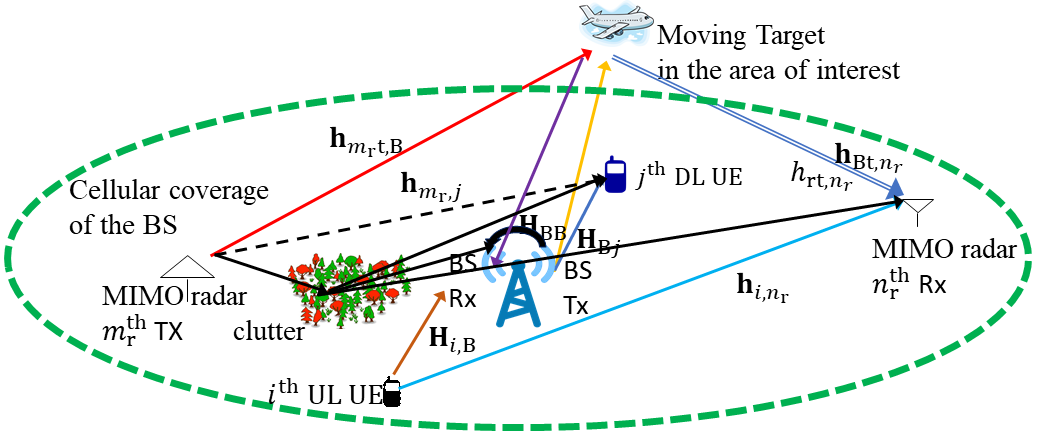
\includegraphics[width=1\columnwidth]{setup_model_tsp.png}
	%\vspace{-pt}
	\caption{Joint spectrum access co-design system model.}
	\vspace{-1em}
\end{figure}
\subsection{Statistical MIMO Radar System Model}
%which consists of a statistical MIMO radar composed of $M_\mathrm{r}$ transmitters (Tx) and $N_\mathrm{r}$ receivers (Rx), a communication BS equipped with $M_\mathrm{c}$ antennas and $\mathit{J}$ active user equipment (UEs), where each UE $\mathit{J}$ is equipped with $\mathit{N}^\textrm{d}_j$ transmit/receive antennas for all $j\in\mathbb{Z}_{+}(J)$. 
% \subsubsection{MIMO Radar Model}\label{mimoradarsys}
%The $M_\mathrm{r}$ Tx and $N_\mathrm{r}$ Rx of the MIMO radar as well as the BS and the $N$ UEs are located in a 2-D plane $\left(x,y \right)$ at coordinates $\left(x_{m_\mathrm{r}},y_{m_\mathrm{r}}\right)$, $m_\mathrm{r}\in{Z}_{+}(M_\mathrm{r})$ and $\left(x_{n_\mathrm{r}},y_{n_\mathrm{r}} \right)$, $n_\mathrm{r}\in\mathbb{Z}_{+}(N_\mathrm{r})$, as well as $(x_{\textrm{B}},y_{\textrm{B}})$ and $(x_{\mathrm{n}},y_{\mathrm{n}})$, $n\in\mathbb{Z}_{+}(N)$, respectively. 

The statistical MIMO radar is composed of $\mathit{M}_\textrm{r}$ single antenna Txs and $\mathit{N}_\mathrm{r}$ Rxs. Within a coherent processing interval (CPI), each element of the MIMO radar Txs transmits a pulse train consisting of $\mathit{K}$ pulses with a pulse repetition interval (PRI) $\mathit{T}_\textrm{r}$, where $\mathit{K}$ is chosen such that the range migration does not occur for the duration of the pulse train\cite{Xiaodong_Overlaid}. The pulse train radiated by the $\ith{m\rr}$ radar Tx is modulated by the waveform code $\mathbf{a}_{k}\in\mathbb{C}^{\mathit{M}\rr}$. We then define the MIMO radar waveform code matrix as $\mathbf{A}\triangleq\bracket{\mathbf{a}^\top\bracket{1};\cdots; \mathbf{a}^\top\bracket{\mathrm{\mathit{K}}}}\in\mathbb{C}^{\mathit{K}\times \mathit{M}\rr}$, where $\mathbf{a}\bracket{k}=\bracket{a_{1}\bracket{k},\cdots,a_{\mathit{M}\rr}\bracket{k}}^\top$ represents the radar codes transmitted during the $\ith{k}$ PRI.	
\iffalse
Each pulse endures the same duration $T_\mathrm{p}\triangleq T_\mathrm{r}/N$ as the symbol duration of the MIMO communications system, where $N\in\mathbb{Z}$ denotes the number of range cells, the pulse train emitted by the $\ith{m_\mathrm{r}}$ Tx can be expressed as\par\noindent\small
\begin{IEEEeqnarray}{rCl}
s_{m_\mathrm{r}}(t)=\sum_{k=1}^{\mathit{K}}a_{m_\mathrm{r},k}\phi_{m_\mathrm{r}}\paren{t-(k-1)T_\mathrm{r}},
\end{IEEEeqnarray}\normalsize
where $\phi_{m_\mathrm{r}}(t)$
%$\tau \in\left[0,T_\textrm{B} \right)$, $k\in \mathbb{Z}(K)$, and $l_\mathrm{s}\in \mathbb{Z}^+(L_\mathrm{s})$ denote the radar Tx antenna index, the fast time, i.e., the time index within one pulse, the slow time, i.e., the index of radar pulse, and the subpulse index, respectively,
denotes the $\ith{m_\mathrm{r}}$ element of the transmit waveform vector $\boldsymbol{\phi}(t)=\left[ \phi_1(t),\dots,\phi_{M_\mathrm{r}}(t)\right]^\top$ that satisfies the following orthonormality condition $\int_{T_\mathrm{p}}^{}\boldsymbol{\phi}(t)\boldsymbol{\phi}^\dagger(t)dt=\mathbf{I}_{M_\mathrm{r}}$.   The overall transmit signals of the MIMO radar can be cast as $\mathbf{s}(t)=\bracket{s_1(t),\cdots,s_{M_\mathrm{r}}(t)}^\top$. Furthermore, the waveforms $\braces{\boldsymbol{\phi}(t)}_{m\rr=1}^{\mathit{M}\rr}$ are narrowband. \cite{MIMOradarseparatedantennas,spacetimecodemimo,MCMIMO_Rad,target_localization}
We first generalize the extended target model developed in the conventional MIMO radar research \cite{MIMOradarseparatedantennas,target_localization,widely_extendedtarget} to facilitate the co-design of MIMO radar and communications system. We consider a near-field scenario for an extended target, distributed radar sensors, BS and the UEs. Each extended target is composed of a large number of independent point-like scatterers, and in contrast to a far-field target, the distance and angle of a near-field target is a function of the transmit and receive element locations as well as the location of the individual scatterer\cite{MIMOradarseparatedantennas}. However, due to the central limit theorem and narrowband transmit signal assumption, 
\fi

The mission of the MIMO radar is to detect a moving target within the radar scene, whose reflectivity factor corresponding to the $\ith{m\rr}$ Tx- $\ith{n\rr}$ Rx pair can be approximately modeled as a CSCG random variable $h_{m\rr \target n\rr }\sim\mathcal{CN}(0,\eta^2_{\target})$, where $\eta^2_{\target}$ denotes the average reflection power of the target and remains constant over the CPI \cite{sun2019target}. If the Doppler frequency observed at the path: $\ith{m\rr}$ radar Tx $\rightarrow$ target $\rightarrow$ $\ith{n\rr}$ radar Rx is denoted by $f^\prime_{m_\mathrm{r}\target n_\mathrm{r}}$, its normalized version can be written as $f_{m_\mathrm{r}\target n_\mathrm{r}}\triangleq f^\prime_{m_\mathrm{r}\target n_\mathrm{r}}\mathit{T}\rr$\cite{hongbin_movingtarget}. We assume that the motion of the target is slow enough such that $f'_{m_\mathrm{r}\target n_\mathrm{r}}$ remains approximately constant within a pulse and fluctuates from pulse to pulse. Denote the target return vector observed at the cell under test (CUT) of the $\ith{n\rr}$ radar Rx by $\mathbf{y}_{\target,n\rr}=\bracket{y_{\mathrm{t},n\rr}\paren{1},\cdots,y_{\mathrm{t},n\rr}\paren{\mathit{K}}}^\top\in\mathbb{C}^{\mathit{K}}$, where $y_{\target,n\rr}\bracket{k}$ can be written as \cite{NaghshTSP2017} \par\noindent\small
\begin{IEEEeqnarray}{rCl}\label{radar range cell}
y_{\mathrm{t},n\rr}\bracket{k}=\mathbf{h}^\top_{\mathrm{rt},n\rr}\mathbf{Q}_{\mathrm{r,}n\rr}\bracket{k}\mathbf{a}\bracket{k},
\end{IEEEeqnarray}\normalsize
where $\mathbf{Q}\rnr\bracket{k}=\diag\paren{\bracket{e^{j2\pi\paren{k-1}f'_{1 \target n\rr}},\cdots,e^{j2\pi\paren{k-1}f'_{\mathit{M}\rr \target n\rr}}}^\top}$.
%and $\mathbf{q}_{\mathrm{r},n\rr}\bracket{k}\triangleq\bracket{e^{j2\pi\paren{k-1}f'_{1 \target n\rr}},\cdots,e^{j2\pi\paren{k-1}f'_{\mathit{M}\rr \target n\rr}}}^\top\in\mathbb{C}^{\mathit{M}\rr}$
%We further define the temporal steering matrix from the $\mathit{M}\rr$ Txs to the $\ith{n\rr}$ Rx as $\mathbf{Q}_{\mathrm{r},n\rr}\triangleq\bracket{\mathbf{q}_{1 \target n\rr},\cdots,\mathbf{q}_{\mathit{M}\rr \target n\rr}}\in\mathbb{C}^{K\times \mathit{M}\rr}$, where the $\ith{m\rr}$ column $\mathbf{q}_{m\rr \target n\rr}=\bracket{1,\cdots,e^{j2\pi\paren{K-1}f'_{m\rr \target n\rr}}}^\top$. 
\iffalse
Next, $y_{\mathrm{r},n\rr}(t)$ is processed by a matched filter bank composed of $\mathit{M}\rr$ filters, where the $\ith{m\rr}$ filter is matched to the waveform $\phi_{m_\mathrm{r}}(t)$ in order to extract the returns due to each MIMO radar transmit element \cite{Vaidyanathan_MIMO_Waveform,MCMIMO_Rad}. The range resolution is set by the pulse length $T_\mathrm{p}$ and each range cell is determined by the peak output of the matched filter through which the received echo signal is passed \cite{richards2010principles}. We also assume the cell synchronization is achieved across the $\mathit{N}\rr$ MIMO radar Rxs and the target is observed at the $\ith{n}$ range cell, i.e., $\lfloor \sfrac{\zeta_{m\rr \target n\rr}}{T_\mathrm{p}}\rfloor=n$ for all $n\rr\in\mathbb{Z}_{+}\paren{\mathit{N}\rr}$. Denoting the matched filter bank output due to the target return at the $\ith{n\rr}$ MIMO radar Rx by $\mathbf{y}_{\mathrm{t},n\rr,n}$, whose $\ith{k}$ element is\par\noindent\small 
\begin{IEEEeqnarray}{rCl}\label{radar range cell}
\mathbf{y}_{\mathrm{t},n\rr,n}\bracket{k}=\mathbf{h}^\top_{\mathrm{rt},n\rr}\mathbf{Q}_{\mathrm{r,}n\rr}\bracket{k}\mathbf{a}\bracket{k}\triangleq\mathbf{h}^\top_{\mathrm{rt},n\rr}\mathbf{s}_{\mathrm{rt,}n\rr}\bracket{k}
\end{IEEEeqnarray}\normalsize
\fi
%$\mathbf{s}_{\textrm{rt},n\rr}=\bracket{\mathbf{Q}\rnr\bracket{1}\mathbf{a}\bracket{1},\cdots,\mathbf{Q}\rnr\bracket{\mathrm{\mathit{K}}}\mathbf{a}\bracket{\mathrm{\mathit{K}}}}$. 

Suggested by \cite{Xiaodong_Overlaid,d2020uplink} that the communications UEs are particularly vulnerable to the undesired reflections or reverberations produced by clutter, we herein utilize the clutter model documented in \cite{NaghshTSP2017}, where the clutter echoes obtained by the $\ith{n\rr}$ radar Rx is regarded as a signal-dependent interfering signal produced by many independent and unambiguous point-like scatterers. The clutter component at the CUT of the $\ith{n\rr}$ radar Rx is denoted by $\mathbf{y}_{\mathrm{c},n\rr}$ with its covariance matrix (CM) being $\mathbf{R}_{\textrm{c},n\rr}\in\mathbb{C}^{\mathit{K}\times \mathit{M}\rr}$, whose $\ith{\paren{m,\ell}}$ element $\mathbf{R}_{\textrm{c},n\rr}\paren{m,\ell}=\sigma^2_{\textrm{c},n\rr}\rho_{\mathrm{c}}^{\lvert m-\ell\rvert}$,
%We consider an exponential correlation shape for $\mathbf{R}_{\textrm{c},n\rr}$, 
\iffalse
\par\noindent\small 
\begin{IEEEeqnarray}{rCl}\label{clutter cov}
\mathbf{R}_{\textrm{c},n\rr}\bracket{m,\ell}=\sigma^2_{\textrm{c},n\rr}\rho^{\lvert m-\ell\rvert}
\end{IEEEeqnarray}\normalsize
\fi
where $\sigma^2_{\textrm{c},n\rr}$ denotes the clutter power observed by the $\ith{n\rr}$ MIMO radar Rx and $\rho$ is a constant\cite{NaghshTSP2017}. 
\subsection{FD MU-MIMO Communications System Model}
For the FD MU-MIMO communications system, the BS equipped with $\mathit{M}_\textrm{c}$ transmit antennas and $\mathit{N}_{\textrm{c}}$ receive antennas operates on the FD mode while $\mathit{I}$ UL and $\mathit{J}$ DL UEs function on the HD mode simultaneously within a scheduling window, where the $\ith{i}$ UL and $\ith{j}$ DL UEs possess $\mathit{N}^{\textrm{u}}_i$ and $\mathit{N}^{\textrm{d}}_j$ transceive antennas, respectively, for all $\braces{i}$ and $\braces{j}$ %$j\in\mathbb{Z}_{+}(\mathit{J})$. 
To potentially achieve the maximum capacity of the UL channels, we suppose $\mathit{M}\cc\geq\sum_{i=1}^{\mathit{I}}\mathit{N}^{\textrm{u}}_i$\cite{MIMOcom}. The co-design of the radar and communications systems allows the length of the scheduling window to be the same as the CPI of the radar system, which indicates that the duration of the CPI should exceed the maximum latency expected by the application \cite{ShiftMIMO}, the length of a UL or DL frame to be identical to the radar PRI, and the UL or DL symbols and the radar pulses to share the same duration. As a result, the number of the frames transmitted in a given window is $\mathit{K}$ and the number of the symbols sent in each frame is $\mathit{N}$. For the simplicity of analysis, the MIMO radar and FD MU-MIMO communications systems are fully synchronous\cite{MCMIMO_RadComm}. 

During the $\ith{l}$ symbol period of the $\ith{k}$ frame, the $\ith{i}$ UL UE sends a unit-energy symbol vector $\mathbf{d}_{\textrm{u},i}\bracket{k,l}\in \mathbb{C}^{d^{\textrm{u}}_i}$ to the BS that is independent and identically distributed (i.i.d.) in $k\in\mathbb{Z}_+\braces{\mathit{K}}$ and $l\in\mathbb{Z}_+\braces{\mathit{N}}$, where $\mathrm{D}^\textrm{u}_i\leq \mathit{N}^{\textrm{u}}_i$ is the number of the data streams. Denoting the precoding matrix utilized by the $\ith{i}$ UL UE during the $\ith{k}$ frame by $\PiB\in\mathbb{C}^{\mathit{N}^{\textrm{u}}_i\times \mathit{D}^\textrm{u}_i}$, the $\ith{i}$ UL UE's transmitted signal vector is thus written as $\mathbf{s}_{\textrm{u},i}\bracket{k,l}=\PiB\mathbf{d}_{\textrm{u},i}\bracket{k,l}$. The UL from the $\ith{i}$ UL UE to the BS is modeled by a Multiple Access Channel (MAC) $\mathbf{H}_{i,\textrm{B}}\in\mathbb{C}^{\mathit{M}\cc\times \mathit{N}^{\textrm{u}}_i}$ and the signal received at the BS due to the transmission of the $\ith{i}$ UL UE is expressed as 
  \par\noindent\small
%\begin{IEEEeqnarray}{rCl} 
\begin{equation}
\label{ULFDcomm}
%\mathbf{y}_{i,\textrm{B}}\bracket{k,l}=\mathbf{H}_{i,\textrm{B}}\PiB\dui.
\mathbf{y}_{i,\textrm{B}}\bracket{k,l}=\mathbf{H}_{i,\textrm{B}}\mathbf{s}_{\textrm{u},i}\bracket{k,l}
%\mathbf{y}_{i,\B}\bracket{k,l}=\sum_{i=1}^I\mathbf{H}_{i,\textrm{B}}\PiB\dui
%\end{IEEEeqnarray}
\end{equation}
\normalsize
The simultaneous transmissions of the rest of UL UEs give rise to the multi-user interference (MUI) for the $\ith{i}$ UL UE, which is shown as  $\mathbf{y}_{\textrm{um},i}\bracket{k,l}=\sum_{q\neq i}\mathbf{H}_{q,\textrm{B}}\mathbf{s}_{\textrm{u},q}\bracket{k,l}$. The CMs of 
$\mathbf{y}_{i,\textrm{B}}\bracket{k,l}$ and $\mathbf{y}_{\textrm{um},i}\bracket{k,l}$ are shown as $\mathbf{R}_{\textrm{u},i}\bracket{k,l}=\HiB\PiB\PiBH\HiBH$ and
$\mathbf{R}_{\textrm{um},i}\bracket{k,l}=\sum_{g\neq i }\mathbf{H}_{g,\textrm{B}}\PBg\PBgH\mathbf{H}^\dagger_{g,\textrm{B}}$.

On the other hand, the $\mathit{J}$ DL UEs download packets from the BS simultaneously. During the $\ith{l}$ symbol period of the $\ith{k}$ frame, the symbol vector intended for the $\ith{j}$ DL UE is denoted by $\mathbf{d}_{\textrm{d},j}\bracket{k,l}\in \mathbb{C}^{\mathrm{D}^\textrm{d}_j}$, i.i.d in $k$ and $l$, where $\mathrm{D}^\textrm{d}_j\leq \min\paren{\mathit{M}\cc,\mathit{N}^{\textrm{d}}_j}$ denotes the number of the unit-energy data streams. %$\mathbf{d}_{\textrm{B},j}\bracket{k,l}$ is also unit-energy, i.e., $\mathbb{E}\bracket{\mathbf{d}_{\textrm{B},j}\bracket{k,l}\mathbf{d}^\dagger_{\textrm{B},j}\bracket{k,l}}=\mathbf{I}_{\mathrm{D}^\textrm{d}_j}$ \cite{Gasussianduality}. %A complex precoding matrix is assigned to each UE to achieve multiple-access interference suppression and spatial diversity exploitation\cite{ArraytoMIMO,ShiftMIMO}. 
Given the precoding matrix for the $\ith{j}$ DL UE at the $\ith{k}$ frame as $\PBj\in\mathbb{C}^{\mathit{M}\cc\times \mathrm{D}^\textrm{d}_j}$, the signal vector transmitted from the BS to the $\ith{j}$ DL UE is written as $\mathbf{s}_{\textrm{d},j}\bracket{k,l}=\PBj\mathbf{d}_{\textrm{\textrm{d}},j}\bracket{k,l}$. The channel between the BS and the $\ith{j}$ DL UE is modeled as a broadcasting (BC) channel $\mathbf{H}_{\textrm{B},j}\in\mathbb{C}^{\mathit{N}^\textrm{d}_j\times \mathit{M}\cc}$, which is also assumed to be full rank for all $j$ to achieve the highest spatial degrees of freedom of the MIMO-BC channel\cite{MIMOcom}. After matched filtering, time/frequency synchronization, and symbol rate sampling, the resulting DL signal received by the $\ith{j}$ DL UE is provided as \par\noindent\small
\begin{flalign}
&\mathbf{y}_{\textrm{B},j}\bracket{k,l}=\mathbf{H}_{\textrm{B},j}\mathbf{s}_{\textrm{d},j}\bracket{k,l}+\mathbf{y}_{\textrm{dm},j}\bracket{k,l},
\end{flalign}\normalsize
where $\mathbf{y}_{\textrm{dm},j}\bracket{k,l}=\mathbf{H}_{\textrm{B},j}\sum_{g\neq j}^{}\mathbf{s}_{\textrm{d},g}\bracket{k,l}$
denotes the MUI of the $\ith{j}$ DL UE. The CMs of $\mathbf{y}_{\textrm{B},j}\bracket{k,l}$ and $\mathbf{y}_{\textrm{dm},j}\bracket{k,l}$ are shown as $\mathbf{R}_{\textrm{dm},j}\bracket{k,l}=\sum_{g\neq j}\mathbf{H}_{\textrm{B},j}\PBg\mathbf{P}^{\dagger}_{\textrm{B},g}\bracket{k}\mathbf{H}^\dagger_{\textrm{B},j}$ and $\mathbf{R}_{\B,j}\bracket{k,l}=\mathbf{R}_{\textrm{dm},j}\bracket{k,l}+ \mathbf{H}_{\textrm{B},j}\PBj\PBjH\mathbf{H}^\dagger_{\textrm{B},j}$, respectively.

Due to the FD transmission of the BS, its Rx is interfered by the DL signals transmitted via the self-interference channel $\mathbf{H}_{\mathrm{BB}}\in{\mathbb{C}^{\mathit{N}\cc\times \mathit{M}\cc}}$ from its Tx. The self-interfering signal at the BS Rx is thus written as 
$\mathbf{y}_{\mathrm{BB}}\bracket{k,l}=\mathbf{H}_{\mathrm{BB}}\sum_{j=1}^{\mathit{J}}\PBj\mathbf{d}_{\textrm{B},j}\bracket{k,l}$. The simultaneous transmissions of the UL and DL UEs allow the $\ith{i}$ UL UE's signals to arrive at the $\ith{j}$ DL UE through the channel $\mathbf{H}_{i,j}\in\mathbb{C}^{\mathit{N}^{\textrm{d}}_j\times \mathit{N}^{\textrm{u}}_i}$, whose CM is $\mathbf{R}_{\mathrm{BB}}\bracket{k,l}=\sum_{j=1}^{\mathit{J}}\mathbf{H}_{\mathrm{BB}}\PBj\PBjH\mathbf{H}^\dagger_\mathrm{BB}$.
%for $i\in\mathbb{Z}^+\braces{\mathit{I}}$ and $j\in\mathbb{Z}^+\braces{\mathit{J}}$
Hence we can write the UL signals received at the $\ith{j}$ DL UE during the $\ith{l}$ symbol period of the $\ith{k}$ frame as $\mathbf{y}_{\mathrm{UL},j}\bracket{k,l}=\sum_{i=1}^{\mathit{I}}\mathbf{H}_{i,j}\PiB\dui$, whose CM is $\mathbf{R}_{\mathrm{UL},j}\bracket{k,l}=\sum_{i=1}^{\mathit{I}}\mathbf{H}_{i,j}\PiB\PiBH\mathbf{H}^\dagger_{i,j}$.
\iffalse
\par\noindent\small
\begin{flalign}
\mathbf{y}_{\mathrm{UL},j}\bracket{k,l}=\sum_{i=1}^{\mathit{I}}\mathbf{H}_{i,j}\PiB\dui,
\end{flalign}\normalsize
\fi
\iffalse
Before proceeding, we define the CMs of $\mathbf{y}_{\textrm{u},i}\bracket{k,l}$, $\mathbf{y}_{\textrm{um},i}\bracket{k,l}$, $\mathbf{y}_{\mathrm{BB}}\bracket{k,l}$, $\mathbf{y}_{\textrm{dm},j}\bracket{k,l}$, $\mathbf{y}_{\textrm{B},j}\bracket{k,l}$ and $\mathbf{y}_{\textrm{UL},j}\bracket{k,l}$ as 
\par\noindent\small
\begin{flalign}
\mathbf{R}_{\textrm{u},i}\bracket{k,l}&=\HiB\PiB\PiBH\HiBH,\nonumber\\
\mathbf{R}_{\textrm{um},i}\bracket{k,l}&=\sum_{g\neq i }\mathbf{H}_{g,\textrm{B}}\PBg\PBgH\mathbf{H}^\dagger_{g,\textrm{B}},\nonumber\\
\mathbf{R}_{\mathrm{BB}}\bracket{k,l}&=\sum_{j=1}^{\mathit{J}}\mathbf{H}_{\mathrm{BB}}\PBj\PBjH\mathbf{H}^\dagger_\mathrm{BB}\nonumber\\
\mathbf{R}_{\textrm{dm},j}\bracket{k,l}&=\sum_{g\neq j}\mathbf{H}_{\textrm{B},j}\PBg\mathbf{P}^{\dagger}_{\textrm{B},g}\bracket{k}\mathbf{H}^\dagger_{\textrm{B},j}\nonumber\\
\mathbf{R}_{\B,j}\bracket{k,l}&=\mathbf{R}_{\textrm{dm},j}\bracket{k,l}+ \mathbf{H}_{\textrm{B},j}\PBj\PBjH\mathbf{H}^\dagger_{\textrm{B},j}\nonumber\\
\mathbf{R}_{\mathrm{UL},j}\bracket{k,l}&=\sum_{i=1}^{\mathit{I}}\mathbf{H}_{i,j}\PiB\PiBH\mathbf{H}^\dagger_{i,j}
\end{flalign}\normalsize
%\fi
%\iffalse
$\mathbf{R}_{\textrm{u},i}\bracket{k,l}=$ $\HiB\PiB\PiBH\HiBH$,  $\mathbf{R}_{\textrm{um},i}\bracket{k,l}=$ $\sum_{g\neq i }\mathbf{H}_{g,\textrm{B}}\PBg\PBgH\mathbf{H}^\dagger_{g,\textrm{B}}$, $\mathbf{R}_{\mathrm{BB}}\bracket{k,l}=$ $\sum_{j=1}^{\mathit{J}}\mathbf{H}_{\mathrm{BB}}\PBj\PBjH\mathbf{H}^\dagger_\mathrm{BB}$, $\mathbf{R}_{\textrm{dm},j}\bracket{k,l}=$ $\sum_{g\neq j}\mathbf{H}_{\textrm{B},j}\PBg\mathbf{P}^{\dagger}_{\textrm{B},g}\bracket{k}\mathbf{H}^\dagger_{\textrm{B},j}$, $\mathbf{R}_{\B,j}\bracket{k,l}=\mathbf{R}_{\textrm{dm},j}\bracket{k,l}+$ $\mathbf{H}_{\textrm{B},j}\PBj\PBjH\mathbf{H}^\dagger_{\textrm{B},j}$, and $\mathbf{R}_{\mathrm{UL},j}\bracket{k,l}=\sum_{i=1}^{\mathit{I}}\mathbf{H}_{i,j}\PiB\PiBH\mathbf{H}^\dagger_{i,j}$, respectively. 
\fi

\subsection{The Radar-Communications Coexistence Model}\label{Coexistence}
We are herein interested in studying the effects that the FD MU-MIMO communications signals lay on the CUT of each radar Rx and the impact of radar probing signals on the UL/DL rates. An overlaid signal diagram for the coexistence model is plotted in \figurename{~\ref{fig:systemmodel}} where $n\in\mathbb{Z}_+\braces{\mathit{L}-1}$ denotes the index for the CUT.  Generally speaking, $\mathbf{s}_{\textrm{d},j}\bracket{k,l}$ reaches the $\ith{n\rr}$ radar Rx through a multi-path fading channel $\mathbf{h}_{\mathrm{Bm},n\rr}\in\mathbb{C}^{\mathit{M}_\mathrm{c}}\sim \mathcal{CN}\paren{0,\eta^2_{\textrm{Bm},n\rr}\mathbf{I}_{\mathit{M}_\mathrm{c}}}$ during the entire CPI. If the time delay between the BS and each radar Rx is negligible, then the DL signals arriving at the $\ith{n\rr}$ radar Rx during the $
\ith{k}$ PRI can be written as \par\noindent\small
\begin{equation*}
y_{\mathrm{Bm},n\rr}\bracket{k}=\mathbf{h}_{\mathrm{Bm},n\rr}^\top e^{j2\pi\paren{k-1} f_{\mathrm{Bm}n_\mathrm{r}}}
\sum_{j=1}^\mathit{J}\mathbf{s}_{\textrm{d},j}\bracket{k,n+1},
\end{equation*}\normalsize
%$y_{\mathrm{Bm},n\rr}\bracket{k}=\mathbf{h}_{\mathrm{Bm},n\rr}^\top e^{j2\pi\paren{k-1} f_{\mathrm{Bm}n_\mathrm{r}}}\sum_{j=1}^\mathit{J}\mathbf{s}_{\textrm{d},j}\bracket{k}$, 
where $f_{\mathrm{Bm}n_\mathrm{r}}$ denotes the corresponding normalized Doppler frequency.  
However, with the presence of the target, the $\ith{n\rr}$ radar Rx can also capture the DL signals reflected off the target through a reflection channel $\mathbf{h}_{\textrm{Bt,}n\rr}\sim\mathcal{CN}\paren{0,\eta^2_{\textrm{Bt},n\rr}\mathbf{I}}$. Without loss of generality, we consider a fully synchronous scenario where $\mathbf{s}_{\textrm{d},j}\bracket{k}$ is reflected off the target before arriving at the CUT of the $\ith{n\rr}$ radar Rx at each PRI through $\mathbf{h}_{\textrm{Bt,}n\rr}$.
With the normalized Doppler frequency being $f_{\textrm{Bt,}n\rr}$, 
\iffalse
their corresponding temporal steering vectors can be written as $\mathbf{q}_{\mathrm{Bm},n\rr}=\bracket{1,\cdots,e^{j2\pi\paren{\mathit{K}-1} f_{\mathrm{Bm}n_\mathrm{r}}}}^\top$ and $\mathbf{q}_{\mathrm{Bt},n\rr}=\bracket{1,\cdots,e^{j2\pi\mathrm{\paren{K-1}}f_{\mathrm{Bt}n_\mathrm{r}}}}^\top$, respectively. 
\fi
the target deflected DL signal observed at the CUT of the $\ith{n\rr}$ radar Rx during the $\ith{k}$ PRI can be written as\par\noindent\small
\begin{equation*}
y_{\mathrm{Bt},n\rr}\bracket{k}=\mathbf{h}_{\mathrm{Bt},n\rr}^\top e^{j2\pi\paren{k-1} f_{\mathrm{Bt}n_\mathrm{r}}}
\sum_{j=1}^\mathit{J}\mathbf{s}_{\textrm{d},j}\bracket{k,1}.
\end{equation*}\normalsize
For the entire CPI, we display the compact forms of $y_{\mathrm{Bm},n\rr}\bracket{k}$ and $y_{\mathrm{Bt},n\rr}\bracket{k}$ as $\mathbf{y}_{\mathrm{Bm},n\rr}\triangleq\bracket{y_{\mathrm{Bm},n\rr}\paren{1},\cdots,y_{\mathrm{Bm},n\rr}\paren{\mathit{K}}}^\top$ and  $\mathbf{y}_{\mathrm{Bt},n\rr}\triangleq\bracket{y_{\mathrm{Bt},n\rr}\paren{1},\cdots,y_{\mathrm{Bt},n\rr}\paren{\mathit{K}}}^\top$, respectively.  
%$\mathbf{S}_{\mathrm{Bm},n\rr}\triangleq$ $\bracket{\mathbf{s}^\top_{\mathrm{Bm},n\rr}\bracket{1};\cdots;\mathbf{s}^\top_{\mathrm{Bm},n\rr}\bracket{\mathrm{\mathit{K}}}}$, $\mathbf{s}_{\mathrm{Bm},n\rr}\bracket{k}=\mathbf{q}_{\mathrm{Bm},n\rr}\bracket{k}\sum_{j=1}^{\mathit{J}}\mathbf{s}_{\textrm{d},j}\bracket{k}$, $\mathbf{S}_{\mathrm{Bt,}n\rr}\triangleq$ $\bracket{\mathbf{s}^\top_{\mathrm{Bt},1}\bracket{1};\cdots;\mathbf{s}^\top_{\mathrm{Bt},n\rr}\bracket{\mathrm{\mathit{K}}}}$ and 
%,$\mathbf{q}_{\mathrm{Bm},n\rr}\bracket{k}=e^{j2\pi\paren{k-1}f_{\mathrm{Bm},n\rr}}$ and$\mathbf{q}_{\mathrm{Bt},n\rr}\bracket{k}=e^{j2\pi\paren{k-1}f_{\mathrm{Bt},n\rr}}$
%, $\mathbf{y}_{\target,n\rr}\triangleq\mathbf{S}_{\target,n\rr}\mathbf{h}_{\target,n\rr}$ and
\begin{figure}[!t]
	%\begin{figure*}[!t]
		\centering
		%	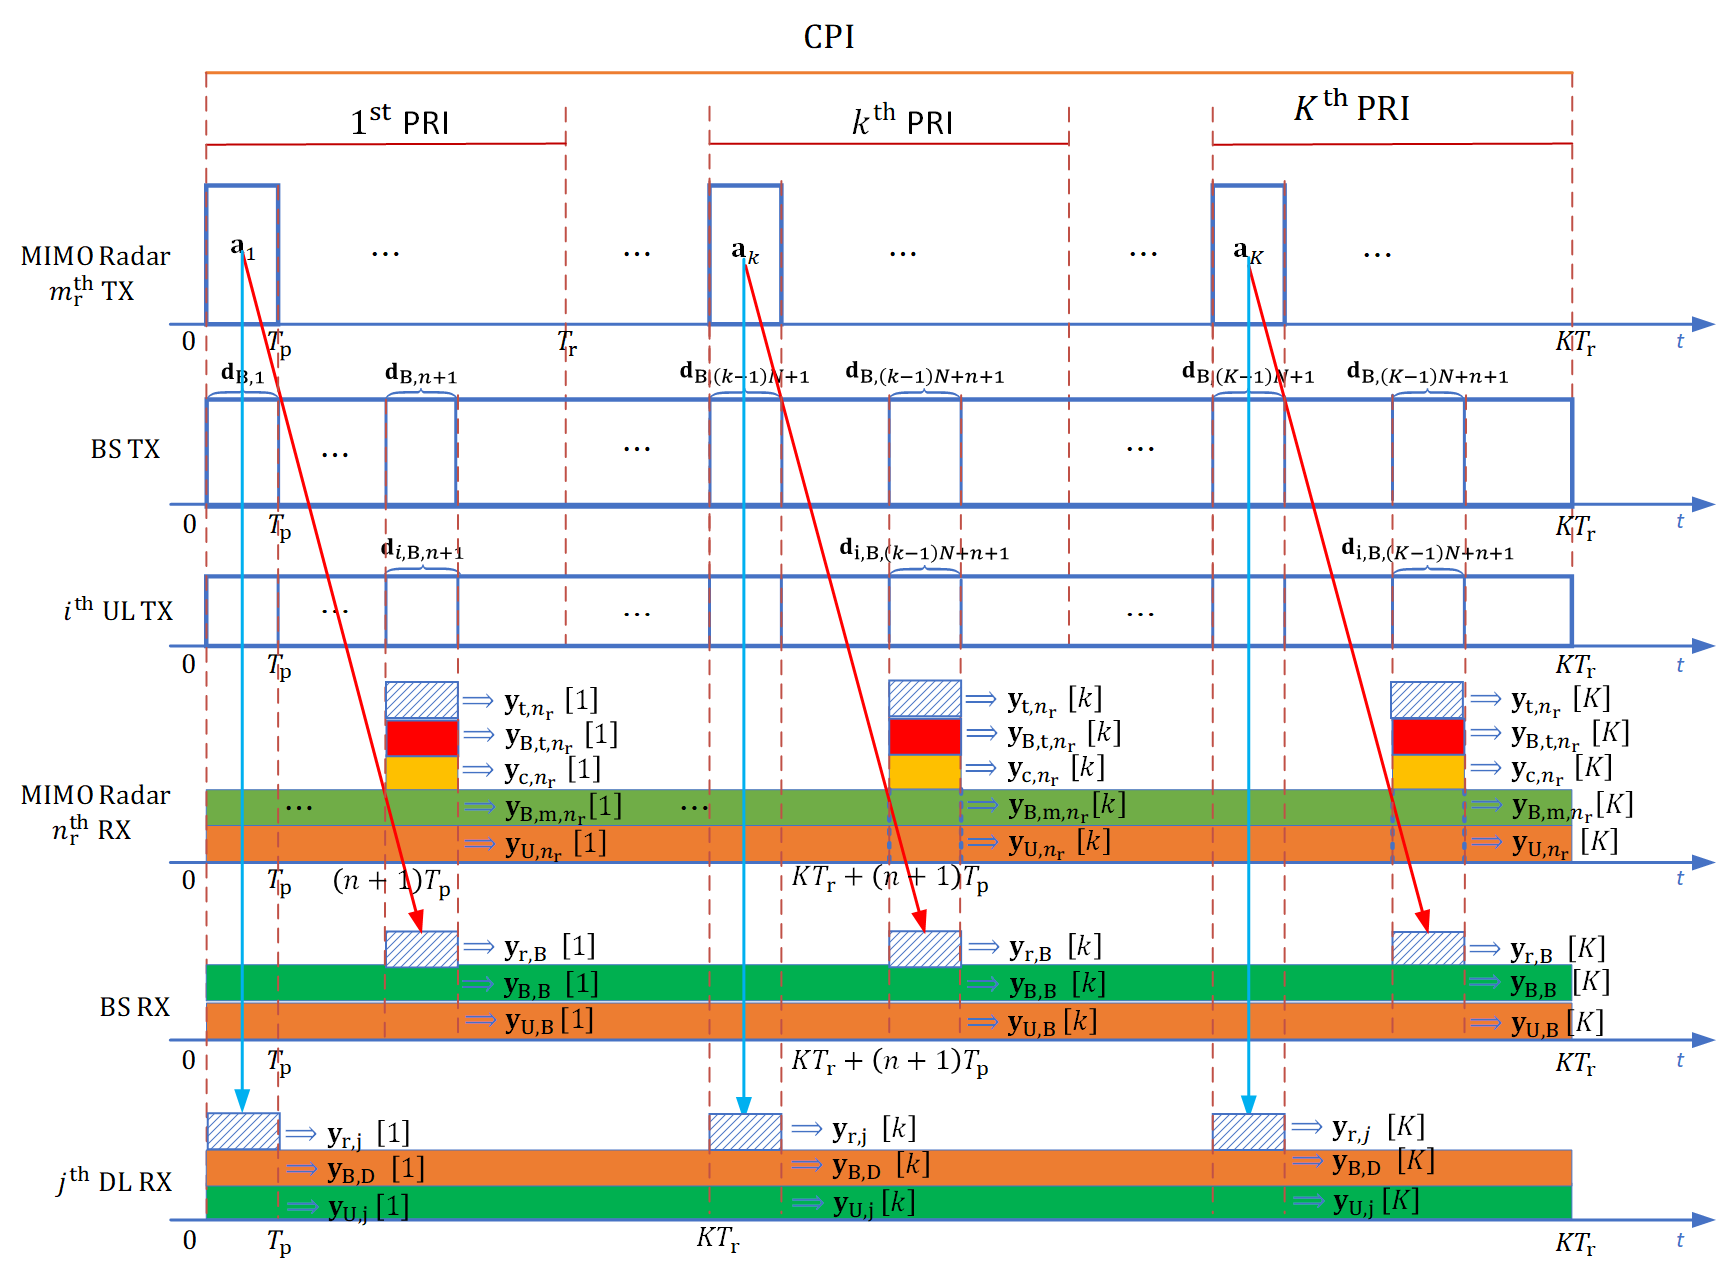
\includegraphics[width=3.1in]{Drawing3}
		%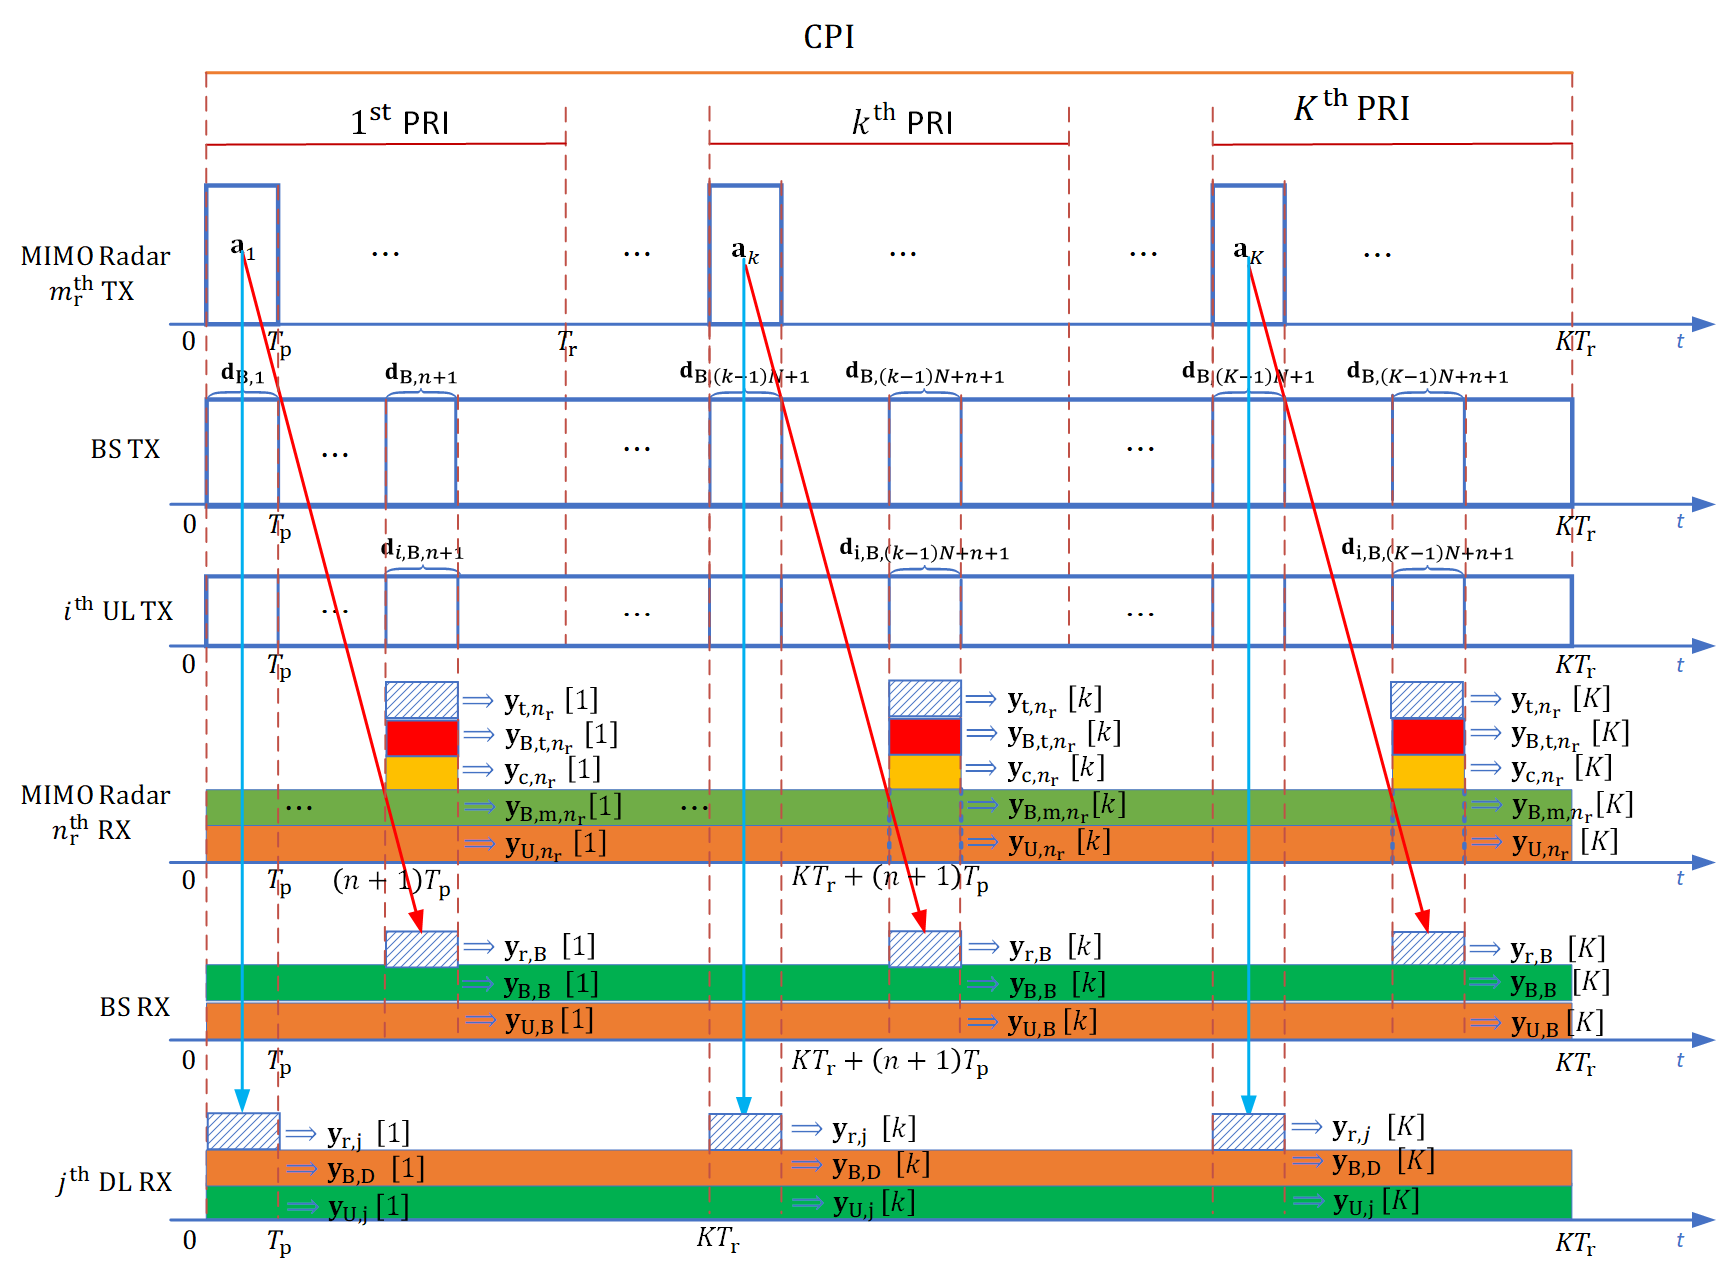
\includegraphics[width=0.80\textwidth]{Drawing3.png}
		%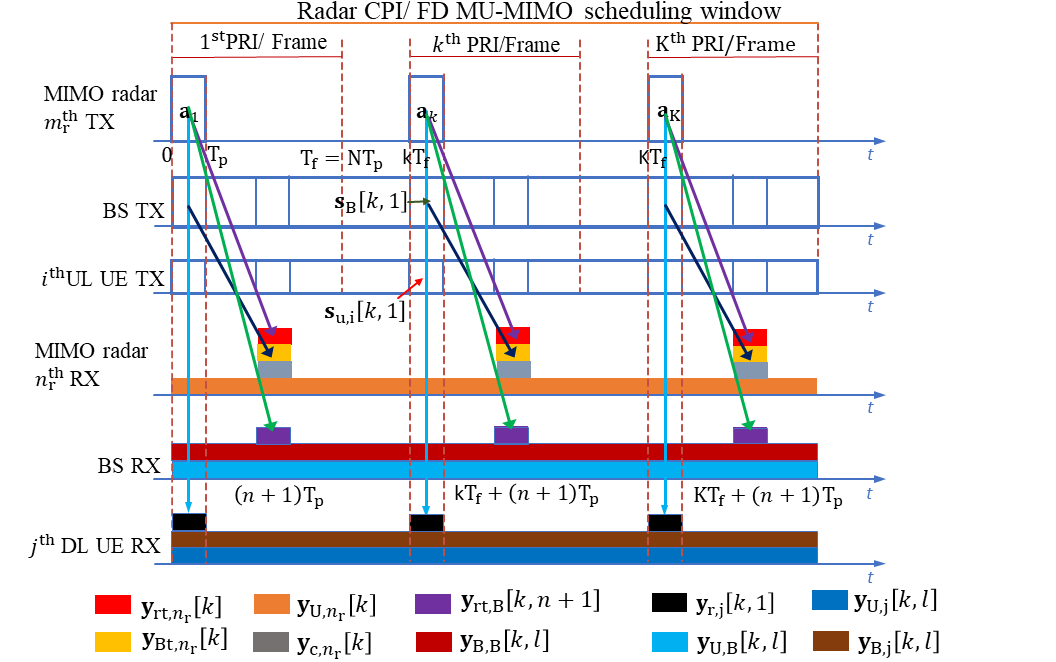
\includegraphics[width=0.80\textwidth]{systemmodel.png}
		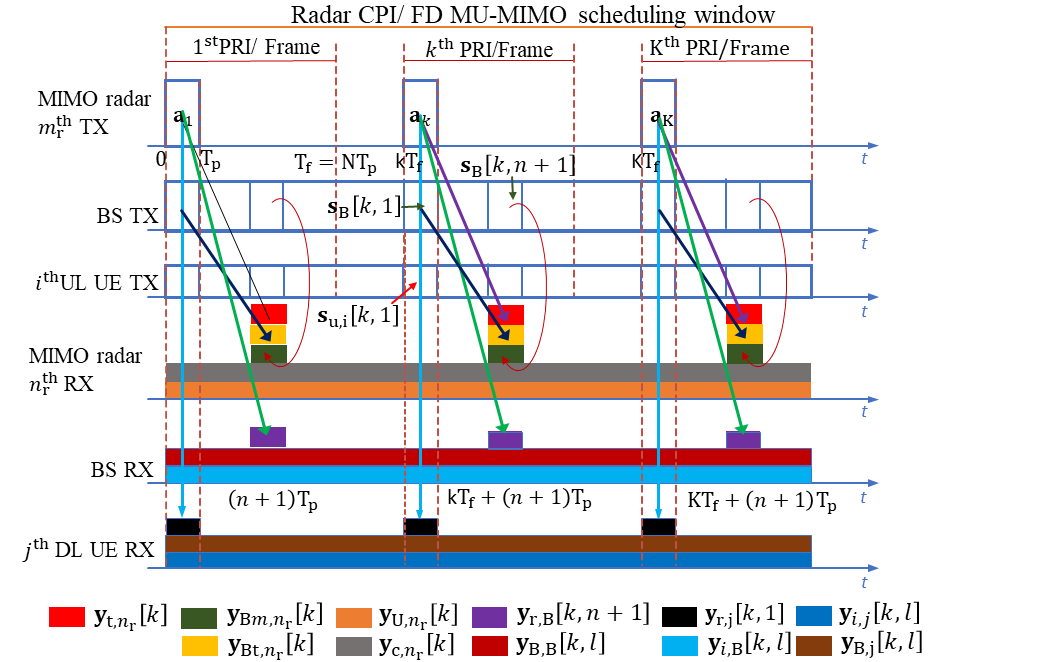
\includegraphics[width=1.0\columnwidth]{system_model_TSP.png}
		\caption{The overlaid signal timing diagram for one CPI is illustrated where the unit time scale is the pulse or symbol duration. For each MIMO radar Rx, we focus on the $\ith{n}$ range cell where the target is observed. The $\ith{j}$ UE is interfered by the radar probing signal during the symbol period when the MIMO radar transmits pulses.} 
		\vspace{-2em}
		\label{fig:systemmodel}
	\end{figure} . %Recall our discussion prior to (\ref{radar range cell}) that our radar system design will be focused on the components in the cell of interest. s

We next define $\mathbf{s}_{\mathrm{rt,}n\rr}\bracket{k}=\mathbf{Q}_{\mathrm{r,}n\rr}\bracket{k}\mathbf{a}\bracket{k}$ and $\mathbf{s}_{\mathrm{Bt},n\rr}\bracket{k}=e^{j2\pi\paren{k-1} f_{\mathrm{Bt}n_\mathrm{r}}}
\sum_{j=1}^\mathit{J}\mathbf{s}_{\textrm{d},j}\bracket{k}$. As $\mathbf{y}_{\textrm{Bt,}n\rr}$ is regarded as the useful signal, the actual number of antennas for detecting the target is $\mathit{M}=\mathit{M}\cc+\MM\rr$, the complete target associated channel matrix as $\mathbf{h}_{\target,n\rr}=\bracket{\mathbf{h}^\top_{\textrm{rt},n\rr},\mathbf{h}^\top_{\textrm{Bt},n\rr}}^\top\in\mathbb{C}^{\mathit{M}}$ whose CM is $\mathbb{E}\bracket{\mathbf{h}_{\target,n\rr}\mathbf{h}^\dagger_{\target,n\rr}}\triangleq\boldsymbol{\Sigma}_{\target,n\rr}=\eta^2_{\textrm{rt},n\rr}\mathbf{I}\oplus\eta^2_{\textrm{Bt},n\rr}\mathbf{I}$, and the total signal vector to detect the target as $\stnrk=\bracket{\mathbf{s}^\top_{\textrm{rt},n\rr}\bracket{k},\mathbf{s}^\top_{\textrm{Bt},n\rr}\bracket{k}}^\top=\mathbf{J}_{\textrm{r}}\srtnrk+\mathbf{J}_{\textrm{B}}\sBtnrk$ where $\mathbf{J}_{\textrm{r}}=\bracket{\mathbf{I}_{\mathit{M}\rr\times \mathit{M}\rr};\mathbf{0}_{\mathit{M}\cc\times \mathit{M}\rr}}\in\mathbb{R}^{\mathbf{\mathit{M}\times \mathit{M}\rr}}$ and $\mathbf{J}_{\textrm{B}}=\bracket{\mathbf{0}_{\mathit{M}\rr\times \mathit{M}\cc};\mathbf{I}_{\mathit{M}\cc\times \mathit{M}\cc}}\in\mathbb{R}^{\mathbf{\mathit{M}\times \mathit{M}\cc}}$, which produce the comprehensive target-reflected signal $$y_{\target,n\rr}\bracket{k}\triangleq\mathbf{h}^\top_{\textrm{rt},n\rr}\mathbf{s}_{\textrm{rt},n\rr}\bracket{k}+\mathbf{h}^\top_{\textrm{Bt},n\rr}\mathbf{s}_{\textrm{Bt},n\rr}\bracket{k}.$$ Denote the CMs of $\mathbf{y}_{\mathrm{Bm},n\rr}$ and $\mathbf{y}_{\mathrm{t},n\rr}$ respectively by $\mathbf{R}_{\textrm{Bm},n\rr}$ and $\mathbf{R}_{\textrm{t},n\rr}$, whose $\ith{\paren{m,l}}$ elements are shown as \par\noindent\small
\begin{align}
&\mathbf{R}_{\mathrm{Bm},n\rr}\paren{m,\ell}\triangleq\mathbb{E}\bracket{y_{\mathrm{Bm},n\rr}\bracket{m}y^\ast_{\mathrm{Bm},n\rr}\bracket{\ell}}\nonumber\\
&=\eta^2_{\textrm{Bm,}n\rr}e^{j2\pi\paren{m-\ell}f_{\mathrm{Bm}n\rr}} \sum_{j=1}^{\mathit{J}}\mathbf{s}^\dagger_{\textrm{d},j}\paren{\ell,n+1}\sum_{j=1}^{\mathit{J}}\mathbf{s}_{\textrm{d},j}\paren{m,n+1}
\end{align}
%\end{align}\normalsize
\begin{align}
%\begin{IEEEeqnarray}{rCl}
&\textrm{and }\mathbf{R}_{\target,n\rr}\paren{m,\ell}\triangleq\mathbb{E}\bracket{y_{\mathrm{t},n\rr}\bracket{m}y^\ast_{\mathrm{t},n\rr}\bracket{\ell}}\nonumber\\
%&=\mathbb{E}\bracket{\mathbf{h}^\top_{\textrm{rt,}n\rr}\mathbf{s}_{\textrm{rt,}n\rr}\bracket{m}\mathbf{s}^\dagger_{\textrm{rt,}n\rr}\bracket{\ell}\mathbf{h}^\ast_{\textrm{rt,}n\rr}}+\mathbb{E}\bracket{\mathbf{h}^\top_{\textrm{Bt,}n\rr}\mathbf{s}_{\textrm{Bt,}n\rr}\bracket{m}\mathbf{s}^\dagger_{\textrm{Bt,}n\rr}\bracket{\ell}\mathbf{h}^\ast_{\textrm{Bt,}n\rr}}\nonumber\\
&=\eta^2_{\textrm{rt,}n\rr}\mathbf{s}^\dagger_{\textrm{rt,}n\rr}\bracket{\ell}\mathbf{s}_{\textrm{rt,}n\rr}\bracket{m}+\eta^2_{\textrm{Bt,}n\rr}\mathbf{s}^\dagger_{\textrm{Bt,}n\rr}\bracket{\ell}\mathbf{s}_{\textrm{Bt,}n\rr}\bracket{m}.
%&=\eta^2_\target \paren{\mathbf{a}^\dagger\bracket{\ell}\mathbf{Q}^\dagger\rnr\bracket{\ell}+\mathbf{q}^\ast_{\mathrm{Bt},n\rr}\bracket{\ell}\sum_{j=1}^J\mathbf{d}^\dagger_{\B,j}\bracket{\ell,1}\mathbf{P}^\dagger_{\B,j}\bracket{\ell}}
%\nonumber\\
%&\cdot\paren{\mathbf{Q}\rnr\bracket{m}\mathbf{a}\bracket{m}+\mathbf{q}_{\mathrm{Bt},n\rr}\bracket{m}\sum_{j=1}^J\PBjm\mathbf{d}_{\B,j}\paren{m,1}},
\end{align}\normalsize
%\end{IEEEeqnarray}
%\begin{align}
%\mathbf{y}_{\mathrm{Bm},n\rr}\bracket{k}&=\mathbf{h}^\top_{\mathrm{Bm},n\rr}\mathbf{s}_{\mathrm{Bm},n\rr}\bracket{k}\nonumber\\
	%&=\mathbf{h}^\top_{\mathrm{Bm},n\rr}\mathbf{q}_{\mathrm{Bm},n\rr}\bracket{k}
	%\sum_{j=1}^J\PBj\mathbf{d}_{\B,j}\bracket{k}
	%\end{align}\normalsize
	%\begin{align}
	%\mathbf{y}_{\mathrm{Bt},n\rr}\bracket{k}=\mathbf{h}^\top_{\mathrm{Bt},n\rr}\mathbf{s}_{\mathrm{Bt},n\rr}\bracket{k}=\mathbf{h}^\top_{\mathrm{Bt},n\rr}\mathbf{q}_{\mathrm{Bt},n\rr}\bracket{k}
	%\sum_{j=1}^J\PBj\mathbf{d}_{\B,j}\bracket{k}
	%\end{align}\normalsize
	
	%$\mathbf{y}_{\mathrm{Bm},n\rr}$ and $\mathbf{y}_{\mathrm{Bt},n\rr}$ can be compactly written as 	
	%\begin{IEEEeqnarray}{rCl} \label{BS-radar multipath}
	%\mathbf{y}_{\mathrm{Bm},n\rr}=\mathbf{Q}_{\mathrm{Bm},n\rr}\mathbf{V}_{\mathrm{Bmr}}\mathbf{h}_{\mathrm{Bm},n\rr} 
	%\end{IEEEeqnarray}
	%and
	%\begin{IEEEeqnarray}{rCl} \label{BS-radar target reflection}
	%\mathbf{y}_{\mathrm{Bt},n\rr}=\mathbf{Q}_{\mathrm{Bt},n\rr}\mathbf{V}_{\mathrm{Btr}}\mathbf{h}_{\mathrm{Bt},n\rr}\triangleq\mathbf{S}_{\mathrm{Bt},n\rr}\mathbf{h}_{\mathrm{Bt},n\rr},
	%\end{IEEEeqnarray}
	%\textcolor{red}{Vijay: matrix S has not been defined.}
	%where $\mathbf{Q}_{\mathrm{Bm},n\rr}=\diag\paren{\mathbf{q}_{\mathrm{Bm},n\rr}}$ and $\mathbf{Q}_{\mathrm{Bt},n\rr}=\diag\paren{\mathbf{q}_{\mathrm{Bt},n\rr}}$.
	%\begin{IEEEeqnarray}{rCl}
	%	\mathit{R}_{\mathrm{Bm},n\rr}\paren{m,\ell}&\triangleq&\mathbb{E}\bracket{\mathbf{y}_{\mathrm{Bm},n\rr}\bracket{m}\mathbf{y}^\dagger_{\mathrm{Bm},n\rr}\bracket{\ell}}\nonumber\\
	%	&=&\eta^2_\B\paren{\sum_{j=1}^{\mathit{J}}\mathbf{d}^\dagger_{\B,j}\bracket{m}\mathbf{P}^\dagger_{\B,j}\bracket{m}}\nonumber\\
	%	&&\cdot\paren{\sum_{j=1}^{\mathit{J}}\PBj\mathbf{d}_{\B,j}\bracket{k}}
	%\end{IEEEeqnarray}
	%$\mathbf{S}_{\mathrm{t},n\rr}\triangleq\mathbf{S}_{\mathrm{rt},n\rr}+\mathbf{S}_{\mathrm{Bt},n\rr}$ 	%$\mathbf{y}_{\mathrm{Bm},n\rr}\bracket{k}=\alpha_{\mathrm{Bt}n_\mathrm{r}}\mathbf{a}^\dagger_\textrm{B}\paren{\theta_{\mathrm{Bt}}}$ %$\mathbf{Y}_{\mathrm{Bmr}}=\bracket{\mathbf{y}_{\mathrm{Bm,}1},\cdots,\mathbf{y}_{\mathrm{Bm,}\mathit{N}\rr}}$ and $\mathbf{Y}_{\mathrm{Btr}}=\bracket{\mathbf{y}_{\mathrm{Bt,}1},\cdots,\mathbf{y}_{\mathrm{Bt,}\mathit{N}\rr}}$ denote the components of $\mathbf{Y}_{\mathrm{Br}}$ through the multipath and target reflection channels, respectively. 
	%where $\zeta_{\textrm{B}\mathrm{m}n\rr}$ denotes the average delay of the multipath channel from the BS to the $\ith{n\rr}$ radar Rx. The co-design of the MIMO radar and FD MU-MIMO communication systems allows $\mathbf{h}_{\textrm{B},n_{\mathrm{r}}}$ to be estimated through the use of training symbols and a priori known.
	%\end{figure*}
	
	%With the narrowband assumption, $\lfloor \sfrac{\zeta_{m\rr \target n\rr }}{T_\mathrm{p}}\rfloor=n$ holds for all $n\rr\in\mathbb{Z}^+\braces{\mathit{N}\rr}$. As shown by the second row of \figurename{$\;$\ref{systemmodel}}, we consider a simplified interference scenario at the radar Rx where the $\ith{n}$ range cell is interfered by $K$ DL and $KI$ UL symbols with the symbol synchronization fully achieved at each sampling point $t=(k-1)T\rr+(n+1)T_\mathrm{p}$. The component of $y_{\textrm{B},n\rr}(t)$ observed at the $\ith{n}$ range cell can be shown as 
	%\begin{IEEEeqnarray}{rCl}
	%	\mathbf{y}_{\textrm{B},n\rr,n}=\sum_{m_\mathrm{r}=1}^{\mathit{M}\rr}\psi_{p,m\rr}(0)\mathbf{s}_{\textrm{B}}\paren{\mathbf{h}_{\textrm{B},n_{\mathrm{r}}}+\mathbf{q}_{n_\mathrm{t},n\rr}},	
	%\end{IEEEeqnarray}
	%where $\psi_{p,m\rr}(0)$ indicates the cross-correlation function of $p\paren{\mathrm{t}}$ and $\phi_{m_\mathrm{r}}(t)$ at lag $0$,  Since the design of $p(t)$ and $\braces{\phi_{m_\mathrm{r}}}_{m\rr=1}^{\mathit{M}\rr}$ is beyond the scope of this paper and term $\sum_{m_\mathrm{r}=1}^{\mathit{M}\rr}\psi_{p,m\rr}(0)$ is a constant once $p(t)$ and $\braces{\phi_{m_\mathrm{r}}}_{m\rr=1}^{\mathit{M}\rr}$ are chosen, we thus do not explicitly show the term $\sum_{m_\mathrm{r}=1}^{\mathit{M}\rr}\psi_{p,m\rr}(0)$ hereafter. Define $\mathbf{Q}_{\mathrm{B,n}\rr}\triangleq\bracket{\mathbf{q}_{\textrm{B},1},\cdots,\mathbf{q}_{\textrm{B},\mathit{N}\rr}}\in\mathbb{C}^{K\times M\cc}$, where the $\ith{n\rr}$ column $\mathbf{q}_{\textrm{B},n\rr}=\bracket{1,\cdots,e^{j2\pi f_{\mathrm{Bt}n_\mathrm{r}}(K-1)T\rr}}^\top$. The matched filter bank output of $y_{\textrm{B},\mathrm{t},n\rr}(t)$ can be given as
	%\begin{equation}
	%\mathbf{y}_{\textrm{B},\mathrm{t},n\rr}=\mathbf{Q}_{\mathrm{B,n}\rr}\odot \mathbf{v}_{\textrm{B}}\mathbf{h}_{\mathrm{Bt},n\rr}
	%C\end{equation}
	
The UL signals are intercepted by the $\ith{n\rr}$ radar Rx throughout the CPI and the ones observed at the CUT of the $\ith{n\rr}$ radar Rx are the $\ith{\paren{n+1}}$ symbols, i.e., $\mathrm{s}_{\textrm{u},i}\bracket{k}$ for all $i$ and $k$. 
%denoted by $\mathbf{S}_{i,n\rr}\triangleq\bracket{\mathbf{s}^\top_{i,n\rr}\paren{1};\cdots;\mathbf{s}^\top_{i,n\rr}\paren{\mathit{K}}}$, where $\mathbf{s}_{i,n\rr}\bracket{k}=\PiB\duin$. 
Unlike the assumption we make on the DL's impact on the radar, we do not consider that $\mathbf{s}_{\textrm{u,}i}\bracket{k,l}$ will reach the radar Rxs through target reflection paths due to a relative small transmission power of the UL UEs. The channel from the $\ith{i}$ UL UE to the $\ith{n\rr}$ MIMO radar Rx is denoted by $\mathbf{h}_{i,n\rr}\sim\mathcal{CN}\paren{0,\eta^2_{i,n\rr}\mathbf{I}_{\mathit{N}^{\textrm{u}}_i}}$, i.i.d in $i$ and $n\rr$. 
The UL signal received at the CUT of the $\ith{n\rr}$ radar Rx during the $\ith{k}$ PRI is \par\noindent\small
\begin{equation*}
y_{\textrm{U},n\rr}\bracket{k}=\sum_{i=1}^{\mathit{I}}\mathbf{h}^\top_{i,n\rr}e^{j2\pi(k-1) f_{i,n_\mathrm{r}}}\mathbf{s}_{\textrm{u},i}\bracket{k},
\end{equation*}
where $f_{i,n_\mathrm{r}}$ denotes the normalized Doppler shift. Combining the entry of $\mathit{K}$ PRI yields the total UL signal observed at the $\ith{n\rr}$ radar Rx as  $\mathbf{y}_{\mathrm{U},n\rr}=\bracket{y_{\textrm{U},n\rr}\paren{1},\cdots,y_{\textrm{U},n\rr}\paren{\mathit{K}}}^\top$ with its CM being $\mathit{R}_{\mathrm{U},n\rr}$, whose
%and temporal steering vector of $\mathbf{S}_{i,n\rr}$ being  and $\mathbf{q}_{i,n\rr}\triangleq\bracket{1,\cdots,e^{j2\pi(k-1) f_{i,n_\mathrm{r}}}}^\top$, respectively, 
$\ith{\paren{m,\ell}}$ entry of the CM of $\mathbf{y}_{\mathrm{U},n\rr}$ is  \par\noindent\small
\begin{align}
%	\begin{IEEEeqnarray}{rCl}
\mathbf{R}_{\mathrm{U},n\rr}\paren{m,\ell}\triangleq&\mathbb{E}\bracket{y_{\mathrm{U},n\rr}\bracket{m}y^\dagger_{\mathrm{U},n\rr}\bracket{\ell}}\nonumber\\
=&\sum_{i=1}^{\mathit{I}}\eta^2_{i,n\rr}e^{j2\pi\paren{m-\ell}f_{i,n\rr}}\mathbf{s}^\dagger_{i,n\rr}\bracket{\ell,n+1}\mathbf{s}_{i,n\rr}\bracket{m,n+1}.
\end{align}\normalsize
Denoting the CSCG noise vector at the $\ith{n\rr}$ radar Rx by $\mathbf{z}\rnr\in\mathcal{CN}\paren{\mathbf{0},\sigma^2\rnr\mathbf{I}}$, we attain the complete receive signal model at the CUT of the $\ith{n\rr}$ MIMO radar Rx as\par\noindent\small
\begin{flalign}
\mathbf{y}\rnr=\mathbf{y}_{\mathrm{t},n\rr}+\underbrace{\mathbf{y}_{\mathrm{c},n\rr}+\mathbf{y}_{\mathrm{Bm},n\rr}+\mathbf{y}_{\mathrm{U},n\rr}+\mathbf{z}\rnr}_{\mathbf{y}^\textrm{r}_{\textrm{in},n\rr}},
\end{flalign}\normalsize
%$\mathbf{y}\rnr=\mathbf{y}_{\mathrm{t},n\rr}+\mathbf{y}_{\text{in},n\rr}$, where $\mathbf{y}_{\text{in},n\rr}=\mathbf{y}_{\mathrm{c},n\rr}+\mathbf{y}_{\mathrm{Bm},n\rr}+\mathbf{y}_{\mathrm{U},n\rr}+\mathbf{z}\rnr$ and $\mathbf{z}\rnr$ denote the interference-plus-noise (IN) component of $\mathbf{y}\rnr$ and CSCG noise vector measured at the $n\rr$ radar Rx. 
where $\mathbf{y}^\textrm{r}_{\textrm{in},n\rr}$ represents the interference-plus-noise (IN) component of $\mathbf{y}\rnr$. The CMs of $\mathbf{y}_{\textrm{in},n\rr}$ and $\mathbf{y}_{\textrm{r},n\rr}$ are respectively given as $\mathbf{R}^\textrm{r}_{\mathrm{in},n\rr}\triangleq\mathbf{R}_{\textrm{c},n\rr}+\mathbf{R}_{\mathrm{Bm},n\rr}+\mathbf{R}_{\mathrm{Ur},n\rr}+\sigma^2\rnr\mathbf{I}$ and $\mathbf{R}_{\textrm{r},n\rr}=\mathbf{R}_{\target,n\rr}+\mathbf{R}^\textrm{r}_{\mathrm{in},n\rr}$. 
% and $\mathbf{R}_{\textrm{r},n\rr}=\mathbf{S}_{\mathrm{t},n\rr}\boldsymbol{\Sigma}_{\target,n\rr}\mathbf{S}^\dagger_{\target,n\rr}+\mathbf{R}_{\mathrm{in},n\rr}$, where 
\iffalse
whose $\ith{\paren{m,\ell}}$ element is \par\noindent\small
	\begin{IEEEeqnarray}{rCl}
		&&\mathbf{R}_{\mathrm{in},n\rr}\paren{m,\ell}\triangleq\mathbb{E}\bracket{\mathbf{y}_{\mathrm{in},n\rr}\bracket{m}\mathbf{y}^\dagger_{\mathrm{in},n\rr}\bracket{\ell}}\nonumber\\
		&=&\mathbf{R}_{\textrm{c},n\rr}\paren{m,\ell}+\mathbf{R}_{\mathrm{Bm},n\rr}\paren{m,\ell}+\mathbf{R}_{\mathrm{U},n\rr}\paren{m,\ell}+\sigma^2\rnr\nonumber\\
		&=&\sigma^2_{\textrm{c},n\rr}\rho^{\lvert m-\ell\rvert}+\eta^2_\B\paren{\sum_{j=1}^{\mathit{J}}\mathbf{d}^\dagger_{\textrm{d},j}\bracket{m}\mathbf{P}^\dagger_{\textrm{d},j}\bracket{m}}\nonumber\\
		&&\cdot\paren{\sum_{j=1}^{\mathit{J}}\mathbf{P}_{\textrm{d},j}\bracket{\ell}\mathbf{d}_{\textrm{d},j}\bracket{l,n+1}}+\sigma^2\rnr+\nonumber\\
		&&+\sum_{i=1}^{\mathit{I}}\eta^2_i\mathbf{d}^\dagger_{\textrm{u},i}\bracket{m}\mathbf{P}^\dagger_{\textrm{u},i}\bracket{m}\mathbf{P}_{\textrm{u},i}\bracket{\ell}\mathbf{d}_{\textrm{u},i}\bracket{l,n+1}.
	\end{IEEEeqnarray}\normalsize
\fi

Over the course of the CPI, the radar probing pulses interfere with the BS and DL UEs intermittently. As shown in \figurename{\;\ref{fig:systemmodel}}, the $\ith{j}$ DL UE receives the radar signals radiated by the $\ith{m\rr}$ radar Tx through a fading channel $\mathbf{h}_{m\rr, j}$ within the $1^{\mathrm{st}}$ symbol period of each frame as plotted in \figurename{$\;$\ref{fig:systemmodel}}. Because of relative small effective antenna apertures of the DL UEs, we do not account the radar signal components scattered by the target at the DL UEs. Denote the channel matrix from the $\mathit{M}\rr$ MIMO radar Txs to the $\ith{j}$ DL UE by $\mathbf{H}_{\mathrm{r},j}\triangleq\bracket{\mathbf{h}_{\mathrm{1},j},\cdots,\mathbf{h}_{\mathit{M}\rr j}}$ and the radar signal intercepted by the $\ith{j}$ DL UE at the $\ith{l}$ symbol period of the $\ith{k}$ frame is written as \par\noindent\small
\begin{equation*}
    \mathbf{y}_{\mathrm{r},j}\bracket{k,l}=
    \begin{cases}
    \mathbf{H}_{\mathrm{r},j}\mathbf{a}_k, \;l=1,\\
    \mathbf{0}, \qquad~~ l\neq1,
    \end{cases}
\end{equation*}
\normalsize
where the Doppler effect of $\mathbf{y}_{\mathrm{r},j}\bracket{k}$ is assumed to be compensated via utilizing the training symbols\cite{MCMIMO_RadComm}. One can proceed to write the non-trivial CM of $\mathbf{y}_{\mathrm{r},j}\bracket{k,l}$ as $\mathbf{R}_{\mathrm{r},j}\bracket{k,1}=\mathbf{H}_{\mathrm{r},j}\mathbf{a}_k\mathbf{a}^\dagger_k\mathbf{H}^\dagger_{\mathrm{r},j}$. The total received signal model of the $\ith{j}$ DL UE is thereby given as 
\begin{equation}
\mathbf{y}_{\textrm{d},j}\bracket{k,l}=\mathbf{y}_{\textrm{B},j}\bracket{k,l}+\mathbf{y}_{\mathrm{U},j}\bracket{k,l}+\mathbf{y}_{\mathrm{r},j}\bracket{k,l}+\mathbf{z}_{\textrm{d},j}\bracket{k,l},
\end{equation}
%\begin{IEEEeqnarray}{rCl} \label{DL UE receive signal discrete}
%	\mathbf{y}_{j}\bracket{k}&=&\mathbf{y}_{\textrm{B},j}\bracket{k}+\mathbf{y}_{\mathrm{U},j}\bracket{k}+\mathbf{y}_{\mathrm{r},j}\bracket{k}+\mathbf{z}_{j}\bracket{k}\IEEEeqnarraynumspace
	%\end{IEEEeqnarray}
where $\mathbf{z}_{\textrm{d},j}\bracket{k,l}$ denotes the CSCG noise vector at the $\ith{j}$ DL UE, i.i.d in $k$ and $l$. The CM of $\mathbf{y}_{\textrm{d},j}\bracket{k,l}$ is shown as $\mathbf{R}^\mathrm{d}_j\bracket{k,l}=\mathbf{R}_{\mathrm{B,j}}\bracket{k,l}+\mathbf{R}^\mathrm{d}_{\mathrm{in,}j}\bracket{k,l}$, where $	\mathbf{R}^\textrm{d}_{\mathrm{in},j}\bracket{k,l}=\mathbf{R}_{\mathrm{dm},j}\bracket{k,l}+\mathbf{R}_{\mathrm{U,}j}\bracket{k,l}+\mathbf{R}_{\mathrm{r},j}\bracket{k,l}+\sigma^2_j\mathbf{I}_{\mathit{N}^{\textrm{d}}_j}$ denotes the IN CM of $\mathbf{y}_{j}\bracket{k,l}$.   %$\mathbf{R}_{\mathrm{Z}_j}\bracket{k}$ where $\mathbf{R}_{\mathrm{Z}_j}=\sigma^2_j\mathbf{I}_{\mathit{N}^{\textrm{d}}_j}$. 
	%Then the overall radar signals observed by the $\ith{j}$ UE during a CPI can be written as $\mathbf{Y}_{\mathrm{r},j}=\mathbf{H}_{\mathrm{r},j}\mathbf{A}^\top$. 
	%We herein conclude the receive signal model of the $\ith{j}$ DL UE as 
	%\begin{equation}
	%\mathbf{Y}_{j}=\mathbf{Y}_{\textrm{B},j}+\mathbf{Y}_{\mathrm{U},j}+\mathbf{Y}_{\mathrm{r},j}+\mathbf{Z}_j
	%\end{equation}
	
Unlike the DL UEs, the BS is equipped with an antenna array with a higher gain and larger aperture such that it can capture the radar signals reflected off the target and clutter. With the far-field assumption held, the target deflected radar signals can be assumed to arrive at the BS Rx during the $\ith{\paren{n+1}}$ symbol period of each frame, and the radar signals returned by the clutter will interfere with the BS throughout the CPI as shown in \figurename{$\;$\ref{fig:systemmodel}}. With the channel matrix between the $\mathit{M}\rr$ MIMO radar Txs and the BS Rx being $\mathbf{H}_{\textrm{rB}}\triangleq\bracket{\mathbf{h}_{1,\textrm{B}},\cdots,\mathbf{h}_{\mathit{M}\rr,\textrm{B}}}\in\mathbb{C}^{\mathit{M}\mathrm{c}\times \mathit{M}\rr}$, the radar signals observed by the BS at the $\ith{l}$ symbol period of the $\ith{k}$ frame is\par\noindent\small
\begin{equation*}
    \mathbf{y}_{\textrm{r,B}}\bracket{k,l}=
    \begin{cases}
    \mathbf{H}_{\mathrm{r},j}\mathbf{a}_k, \;l=n+1,\\
    \mathbf{0}, \qquad~~ l\neq n+1,
    \end{cases}
\end{equation*}
\normalsize
whose non-trivial CM is given as $\mathbf{R}_{\mathrm{r,B}}\bracket{k}=\mathbf{H}_{\textrm{rB}}\mathbf{a}_k\mathbf{a}^\dagger_k\mathbf{H}^\dagger_{\textrm{rB}}$. With the CSCG noise vector measured at the BS Rx $\mathbf{z}_\textrm{B}\bracket{k,l}\sim\mathcal{CN}\paren{0,\sigma^2_{\textrm{B}}\mathbf{I}_{M\cc}}$, the resultant received signal model at the BS Rx to decode $\mathbf{s}_{\textrm{u},i}\bracket{k,l}$ is shown as 
\begin{equation*}
    \mathbf{y}_{\textrm{u},i}\bracket{k,l}=\mathbf{y}_{i,\B}\bracket{k,l}+\mathbf{y}_{\textrm{um},i}\bracket{k,l}+\mathbf{y}_{\textrm{BB}}\bracket{k,l}+\mathbf{y}_{\textrm{rB}}\bracket{k,l}+\mathbf{z}_\textrm{B}\bracket{k,l}.
\end{equation*}
	%\begin{IEEEeqnarray}{rCl}\label{UL_comm receiv signal cont}
	%	\mathbf{y}_{i}\paren{k,\ell}&=&\sum_{i=1}^I\mathbf{y}_{i,\B}\paren{k,\ell}+\mathbf{y}_{\mathrm{BB}}\paren{k,\ell}\nonumber\\
	%	&&\>+\mathbf{y}_{\textrm{rB}}\paren{k,\ell}+\mathbf{z}_\textrm{B}\paren{k,\ell}, 
	%\end{IEEEeqnarray}
We then obtain the CMs of the IN of the $\ith{i}$ UL UE as $\mathbf{R}^\textrm{u}_{\mathrm{in},i}\bracket{k,l}=\mathbf{R}^\textrm{u}_{\textrm{um}, i}\bracket{k,l}+\mathbf{R}_{\mathrm{BB}}\bracket{k,l}+\mathbf{R}_{\textrm{rB}}\bracket{k,l}+\sigma^2_{\textrm{B}}\mathbf{I}_{\mathit{M}\cc}$ and the CM of $\mathbf{y}_{\textrm{u},i}\bracket{k,l}$ as $\mathbf{R}^\mathrm{u}_{i}\bracket{k,l}\triangleq\mathbf{R}_{i,\B}\bracket{k,l}+\mathbf{R}^\textrm{u}_{\mathrm{in},i}\bracket{k,l}$. 

For the rest of our discussion, we consider that $\mathbf{H}_{\textrm{B},j}$, $\mathbf{H}_{i,\textrm{B}}$, $\mathbf{H}_{i,j}$, and $\mathbf{H}_{\textrm{B,B}}$ are Rayleigh fading channels with the channel gains $\eta^2_{\textrm{d},j}$, $\eta^2_{\textrm{u},i}$, $\eta^2_{i,j}$, and $\eta^2_{\textrm{BB}}$, respectively, for all $\braces{i,j}$, and the radar interfering channels to the BS and UL UEs are modeled as Rician vectors, i.e.,  $\mathbf{h}_{m\rr,\textrm{B}}\sim\mathcal{CN}\paren{\sqrt{\frac{\kappa}{\kappa+1}}\boldsymbol{\mu}_{m\rr,\textrm{B}},\frac{\eta^2_\mathrm{m\rr}}{\kappa+1}\mathbf{I}_{\mathit{N}^{\textrm{d}}_j}}$ and $\mathbf{h}_{m\rr, j}\sim\mathcal{CN}\paren{\sqrt{\frac{\kappa}{\kappa+1}}\boldsymbol{\mu}_j,\frac{\eta^2_j}{\kappa+1}\mathbf{I}_{\mathit{N}^{\textrm{d}}_j}}$, where $\kappa$ denotes the $K$-factor, $\boldsymbol{\mu}_{m\rr,\textrm{B}}$ and $\boldsymbol{\mu}_{m\rr,j}$ the specular path gains, and $\eta^2_{m\rr,\textrm{B}}$ and $\eta^2_{m\rr,j}$ the variances of the scattered paths, for all $\braces{m\rr,j}$.  We assume that CSIT, CSIR as well as the second-order statistics of $h_{m\rr\textrm{t}n\rr}$ and $\mathbf{h}_{\textrm{Bt},n\rr}$, i.e., $\eta^2_{\textrm{rt},n\rr}$ and $\eta^2_{\textrm{Bt},n\rr}$ are perfectly known by the BS, all the UEs and the MIMO radar Rxs. 

As $\mathbf{y}_{\mathrm{r,B}}\bracket{k,l}$ and $\mathbf{y}_{\mathrm{r},j}\bracket{k,l}$ are only non-trivial when $l=n+1$ and $l=1$, respectively, we concentrate on studying the DL and UL performances at the $\ith{\paren{n+1}}$ and $1^{\textrm{st}}$ symbol periods of each frame, respectively, for the spectral co-design. To lighten the burden of the notation, we omit the symbol period index $l$ for the rest of the paper.
\section{Problem Formulation}
\label{sec: formulation}
In this section, we derive the CWSM expression before formulating the CWSM maximization problem based on the proposed spectral co-design model in Section \ref{sec:system}. Radar and communications system designs normally demand different performance characteristics. The MI has been a well understood metric in MU-MIMO communications for transmit precoder design\cite{WMMSEWSR} and ever since the seminal work on MI as a radar waveform design metric by \cite{Bellinformation}, and the MI has become a common criterion for the MIMO radar waveform design \cite{Jammer_game,NaghshTSP2017}. It has been shown that maximizing the MI between the radar received signal and the target response leads to a better detection performance in the presence of the Gaussian noise\cite{Jammer_game}. 
%In this work, the MI of the MIMO radar is defined as the MI between the output of the linear receiver and the channel target response. 
	
%The co-design of the MIMO radar transceiver involves applying a linear receive filter bank at each MIMO radar Rx. Denote the receiver of the $\ith{n\rr}$ Rx by $\mathbf{U}_{\mathrm{r},n\rr}\in\mathbb{C}^{\mathit{M}\rr\times K}$ whose output  $\widetilde{\mathbf{y}}\rnr$ is\par\noindent\small
	%\begin{IEEEeqnarray}{rCl}
	%\widetilde{\mathbf{y}}\rnr&=&\mathbf{U}\rnr\mathbf{y}\rnr\nonumber\\
	%&=&\mathbf{U}\rnr\paren{\mathbf{S}_{\mathrm{rt},n\rr}\mathbf{h}_{\mathrm{rt},n\rr}+\mathbf{S}_{\mathrm{Bt},n\rr}\mathbf{h}_{\mathrm{Bt},n\rr}}+\widetilde{\mathbf{y}}_{\mathrm{in},n\rr}
	%\end{IEEEeqnarray}\normalsize
	%where $\widetilde{\mathbf{y}}_{\mathrm{in},n\rr}=\mathbf{U}\rnr\mathbf{y}_{\mathrm{in},n\rr}$. %\textcolor{red}{matrices $\mathbf{U}$ have never been defined earlier?}. 
	%As we assume that both
	%As $\mathbf{h}_{\mathrm{rt},n\rr}$ and $\mathbf{h}_{\mathrm{Bt},n\rr}$ contain target information, the conditional MI between $\widetilde{\mathbf{y}}\rnr$ and jointly $\mathbf{h}_{\mathrm{rt},n\rr}$ and $\mathbf{h}_{\mathrm{Bt},n\rr}$ given the radar transmit codes $\mathbf{A}$ can be written as\par\noindent\small
	%\begin{IEEEeqnarray}{rCl}
	%\mathit{I}\rnr&\triangleq&\mathit{I}\paren{\widetilde{\mathbf{y}}\rnr;\mathbf{h}_{\mathrm{rt},n\rr},\mathbf{h}_{\mathrm{Bt},n\rr}|\mathbf{A}}\nonumber\\
	%&=&I\paren{\widetilde{\mathbf{y}}\rnr;\mathbf{h}_{\mathrm{rt},n\rr}|\mathbf{A}}+I\paren{\widetilde{\mathbf{y}}\rnr;\mathbf{h}_{\mathrm{Bt},n\rr}|\mathbf{h}_{\mathrm{rt},n\rr},\mathbf{A}}\nonumber%\\
	%&=&\mathit{H}\paren{\widetilde{\mathbf{y}}\rnr|\mathbf{A}}-\mathit{H}\paren{\widetilde{\mathbf{y}}\rnr|\mathbf{h}_{\mathrm{rt},n\rr},\mathbf{h}_{\mathrm{Bt},n\rr},\mathbf{A}}\nonumber\\
	%&=&\mathit{H}\paren{\widetilde{\mathbf{y}}\rnr|\mathbf{A}}-\mathit{H}\paren{\widetilde{\mathbf{y}}_{\mathrm{in},n\rr}|\mathbf{A}}
	%\end{IEEEeqnarray}\normalsize
	%where $\mathit{H}\paren{\widetilde{\mathbf{y}}\rnr|\mathbf{A}}$ and  $\mathit{H}\paren{\widetilde{\mathbf{y}}_{\mathrm{in},n\rr}|\mathbf{A}}$ denote the conditional differential entropies of $\widetilde{\mathbf{y}}\rnr$ given $\mathbf{A}$ and $\widetilde{\mathbf{y}}_{\mathrm{in},n\rr}$, respectively, and the last equality is because after observing $\mathbf{h}_{\mathrm{rt},n\rr}$ and $\mathbf{h}_{\mathrm{Bt},n\rr}$, the only uncertainty remaining in $\widetilde{\mathbf{y}}\rnr$ is due to $\widetilde{\mathbf{y}}_{\text{in},n\rr}$, and since $\mathbf{y}_{\text{in},n\rr}$ and $\mathbf{h}_{\mathrm{rt},n\rr}$ as well as $\mathbf{h}_{\mathrm{Bt},n\rr}$ are independent, the last equality holds. By the definition of the conditional differential entropy with the Gaussian noise, one can obtain that \cite{cover2012elements}\par\noindent\small
	%\begin{IEEEeqnarray}{rCl}
	%\mathit{H}\paren{\widetilde{\mathbf{y}}\rnr|\mathbf{A}}&=&\rho+\log\left|\mathbf{U}\rnr\mathbf{R}_{\mathrm{r},n\rr}\mathbf{U}^\dagger\rnr \right|\\
	%\mathit{H}\paren{\widetilde{\mathbf{y}}_{\mathrm{in},n\rr}|\mathbf{A}}&=&\rho+\log\left|\mathbf{U}\rnr\mathbf{R}_{\mathrm{in},n\rr}\mathbf{U}^\dagger\rnr \right|
	%\end{IEEEeqnarray}\normalsize
	%where the constant $\rho=K\log\paren{\pi}+K$. This leads to\par\noindent\small
	%\begin{IEEEeqnarray}{rCl}\label{radarmi}
	%\mathit{I}\rnr&=&\log\frac{\left|\mathbf{U}\rnr\paren{\mathbf{R}_{\mathrm{rt},n\rr}+\mathbf{R}_{\mathrm{Bt},n\rr}+\mathbf{R}_{\mathrm{in},n\rr}}\mathbf{U}^\dagger\rnr \right|}{\left|\mathbf{U}\rnr\mathbf{R}_{\mathrm{in},n\rr}\mathbf{U}^\dagger\rnr \right|}\nonumber\\
	%&=&\log\left|
	%\sizecorr{\paren{\mathbf{U}\rnr\mathbf{R}_{\mathrm{in},n\rr}\mathbf{U}^\dagger\rnr}^{-1}}
	%\mathbf{I}+\mathbf{U}\rnr\paren{\mathbf{R}_{\mathrm{rt},n\rr}+\mathbf{R}_{\mathrm{Bt},n\rr}}\mathbf{U}^\dagger\rnr\right.\nonumber\\
	%&&\left.\paren{\mathbf{U}\rnr\mathbf{R}_{\mathrm{in},n\rr}\mathbf{U}^\dagger\rnr}^{-1}\right|
	%\end{IEEEeqnarray}\normalsize
	%With $\mathbf{h}_{\mathrm{rtr}}\triangleq\vect\braces{\mathbf{H}_{\mathrm{rtr}}}$ and $\mathbf{h}_{\mathrm{Btr}}\triangleq\vect\braces{\mathbf{H}_{\mathrm{Btr}}}$, the resulting MI between $\widetilde{\mathbf{y}}\rr=\sum_{n\rr=1}^{\mathit{N}\rr}\widetilde{\mathbf{y}}\rnr$ and, jointly $\mathbf{h}_{\mathrm{rtr}}$ and $\mathbf{h}_{\mathrm{Btr}}$ is \par\noindent\small
	%\begin{IEEEeqnarray}{rCl}
	%I\rr&\triangleq&\mathit{I}\paren{\mathbf{y}\rr;\mathbf{h}_{\mathrm{rtr}},\mathbf{h}_{\mathrm{Btr}}|\mathbf{A}}=\sum_{n\rr=1}^{\mathit{N}\rr}\mathit{I}\rnr
	%\end{IEEEeqnarray}\normalsize
	%\begin{IEEEeqnarray}{rCl}\label{radarmi}
	%\mathit{I}\paren{\mathbf{y}\rr;\mathbf{h}_{\mathrm{rt},n\rr},\mathbf{h}_{\mathrm{Bt},n\rr}|\mathbf{A}}&=&\log\frac{\left|\mathbf{R}_{\mathrm{rt},n\rr}+\mathbf{R}_{\mathrm{Bt},n\rr}+\mathbf{R}_{\mathrm{in},n\rr} \right|}{\left|\mathbf{R}_{\mathrm{in},n\rr} \right|}\nonumber\\
	%&=&\log\left|\mathbf{I}_{KN\rr}+\mathbf{R}^{-1}_{\mathrm{in,r}}\paren{\mathbf{R}_{\mathrm{rt},n\rr}+\mathbf{R}_{\mathrm{Bt},n\rr}}\right|. \IEEEeqnarraynumspace
	%\end{IEEEeqnarray}
	%and we define $\mathbf{W}^{\mathrm{MMSE}}_{\textrm{B},k}\triangleq\mathbf{W}^{\mathrm{MMSE}}_{\textrm{B},\paren{k-1}N+n+1}$ to lighten the notation. 
To derive CWSM, we first denote the linear receive filter at the $\ith{n\rr}$ MIMO radar Rx by $\mathbf{U}_{\mathrm{r},n\rr}\triangleq\bracket{\mathbf{u}_{\textrm{r},n\rr}\paren{1},\cdots,\mathbf{u}_{\textrm{r},n\rr}\paren{\mathit{K}}}\in\mathbb{C}^{\MM\times\mathrm{\mathit{K}}}$ and define $\mathbf{S}_{\target,n\rr}=\bracket{\mathbf{s}_{\textrm{t},n\rr}\paren{1},\cdots,\mathbf{s}_{\textrm{t},n\rr}\paren{\mathrm{\mathit{K}}}}$. The output of $\mathbf{U}_{\mathrm{r},n\rr}$ can be shown as \par\noindent\small
\begin{IEEEeqnarray}{rCl}
%	\widetilde{\mathbf{y}}_{\textrm{r},n\rr}&=&\mathbf{U}\rnr\paren{\mathbf{s}_{\textrm{rt},n\rr}\mathbf{h}_{\mathrm{rt},n\rr}+\mathbf{s}_{\textrm{Bt},n\rr}\mathbf{h}_{\mathrm{Bt},n\rr}}+\mathbf{U}\rnr\mathbf{y}_{\textrm{in},n\rr}\nonumber\\
\widetilde{\mathbf{y}}_{\textrm{r},n\rr}&=&\underbrace{\mathbf{U}\rnr\mathbf{S}_{\textrm{t},n\rr}\mathbf{h}_{\mathrm{t},n\rr}}_{\widetilde{\mathbf{y}}_{\textrm{t},n\rr}}+  \underbrace{\mathbf{U}\rnr\mathbf{y}_{\textrm{in},n\rr}}_{\widetilde{\mathbf{y}}_{\textrm{in},n\rr}}\nonumber\\
&=& \sum_{k=1}^{\mathit{K}}\urk\braces{\mathbf{y}_{\textrm{t},n\rr}\bracket{k}+\mathbf{y}_{\textrm{in},n\rr}\bracket{k}}.
\end{IEEEeqnarray}\normalsize
As $\mathbf{h}_{\mathrm{t},n\rr}$ contains the target information, the conditional MI between $\widetilde{\mathbf{y}}_{\textrm{r},n\rr}$ and 
%jointly $\mathbf{h}_{\mathrm{rt},n\rr}$ and
$\mathbf{h}_{\mathrm{t},n\rr}$ given the radar waveform code matrix $\mathbf{A}$ using chain rules can be written as \cite{cover2012elements}\par\noindent\small
\begin{IEEEeqnarray}{rCl}
\mathit{I}\rnr&\triangleq&\mathit{I}\paren{\widetilde{\mathbf{y}}\rnr;\mathbf{h}_{\mathrm{t},n\rr}|\mathbf{A}}\nonumber\\
%&=&I\paren{\widetilde{\mathbf{y}}\rnr;\mathbf{h}_{\mathrm{rt},n\rr}|\mathbf{A}}+I\paren{\widetilde{\mathbf{y}}\rnr;\mathbf{h}_{\mathrm{Bt},n\rr}|\mathbf{h}_{\mathrm{rt},n\rr},\mathbf{A}}\nonumber\\
&=&\mathit{H}\paren{\widetilde{\mathbf{y}}\rnr|\mathbf{A}}-\mathit{H}\paren{\widetilde{\mathbf{y}}\rnr|\mathbf{h}_{\mathrm{t},n\rr},\mathbf{A}}\nonumber\\
&=&\mathit{H}\paren{\widetilde{\mathbf{y}}\rnr|\mathbf{A}}-\mathit{H}\paren{\widetilde{\mathbf{y}}_{\textrm{t},n\rr}|\mathbf{h}_{\mathrm{t},n\rr},\mathbf{A}}-\mathit{H}\paren{\widetilde{\mathbf{y}}_{\mathrm{in},n\rr}|\mathbf{h}_{\mathrm{t},n\rr},\mathbf{A}}\nonumber\\
&=&\mathit{H}\paren{\widetilde{\mathbf{y}}\rnr|\mathbf{A}}-\mathit{H}\paren{\widetilde{\mathbf{y}}_{\mathrm{in},n\rr}|\mathbf{A}},
\end{IEEEeqnarray}\normalsize
where the last equality holds because $\widetilde{\mathbf{y}}_{\mathrm{in},n\rr}$ completely depends on $\mathbf{A}$ such that $\mathit{H}\paren{\widetilde{\mathbf{y}}_{\textrm{t},n\rr}|\mathbf{h}_{\mathrm{t},n\rr}}$  and $\mathbf{h}_{\mathrm{t},n\rr}$ as well as  $\widetilde{\mathbf{y}}_{\textrm{in},n\rr}$ and $\mathbf{h}_{\textrm{tt},n\rr}$ are mutually independent. By the definition of the conditional differential entropy with the Gaussian noise, one can obtain that \cite{cover2012elements} \par\noindent\small
\begin{IEEEeqnarray}{rCl}
\mathit{H}\paren{\widetilde{\mathbf{y}}\rnr|\mathbf{A}}&=&\varrho+\log\left|\mathbf{U}\rnr\mathbf{R}_{\mathrm{r},n\rr}\mathbf{U}^\dagger\rnr \right|,\nonumber\\
\mathit{H}\paren{\widetilde{\mathbf{y}}_{\mathrm{in},n\rr}|\mathbf{A}}&=&\varrho+\log\left|\mathbf{U}\rnr\mathbf{R}_{\mathrm{in},n\rr}\mathbf{U}^\dagger\rnr \right|,\nonumber
\end{IEEEeqnarray}\normalsize
where the constant $\varrho=K\log\paren{\pi}+K$. This leads to\par\noindent\small
\begin{IEEEeqnarray}{rCl}\label{radarmi}
	\mathit{I}\rnr&=&\log\frac{\left|\mathbf{U}\rnr\paren{\mathbf{R}_{\mathrm{t},n\rr}+\mathbf{R}_{\mathrm{in},n\rr}}\mathbf{U}^\dagger\rnr \right|}{\left|\mathbf{U}\rnr\mathbf{R}_{\mathrm{in},n\rr}\mathbf{U}^\dagger\rnr \right|}\nonumber\\
	&=&\log\left\lvert\mathbf{I}+\mathbf{U}\rnr\mathbf{R}_{\textrm{t},n\rr}\mathbf{U}^\dagger\rnr\paren{\mathbf{U}\rnr\mathbf{R}_{\mathrm{in},n\rr}\mathbf{U}^\dagger\rnr}^{-1}\right\rvert.
	%&=&\log\left|
	% \sizecorr{\paren{\mathbf{U}\rnr\mathbf{R}_{\mathrm{in},n\rr}\mathbf{U}^\dagger\rnr}^{-1}}
	%\mathbf{I}+\mathbf{U}\rnr\mathbf{R}_{\textrm{t},n\rr}\mathbf{U}^\dagger\rnr\right.\nonumber\\
	%&&\left.\paren{\mathbf{U}\rnr\mathbf{R}_{\mathrm{in},n\rr}\mathbf{U}^\dagger\rnr}^{-1}\right|. 
\end{IEEEeqnarray}\normalsize
\iffalse
With $\mathbf{h}_{\mathrm{rtr}}\triangleq\vect\braces{\mathbf{H}_{\mathrm{rtr}}}$ and $\mathbf{h}_{\mathrm{Btr}}\triangleq\vect\braces{\mathbf{H}_{\mathrm{Btr}}}$, the resulting MI between $\widetilde{\mathbf{y}}\rr=\sum_{n\rr=1}^{\mathit{N}\rr}\widetilde{\mathbf{y}}\rnr$ and, jointly $\mathbf{h}_{\mathrm{rtr}}$ and $\mathbf{h}_{\mathrm{Btr}}$ is \par\noindent\small
\begin{IEEEeqnarray}{rCl}
	I\rr&\triangleq&\mathit{I}\paren{\mathbf{y}\rr;\mathbf{h}_{\mathrm{rtr}},\mathbf{h}_{\mathrm{Btr}}|\mathbf{A}}=\sum_{n\rr=1}^{\mathit{N}\rr}\mathit{I}\rnr
\end{IEEEeqnarray}\normalsize	
\fi
The linear receive filters deployed at the BS for the $\ith{i}$ UL UE and the $\ith{j}$ DL UE during the $\ith{k}$ frame are denoted by $\UiB\in\mathbb{C}^{\mathrm{d}^\textrm{u}_i\times \mathit{N}\cc}$ and $\UBj\in\mathbb{C}^{\mathrm{d}^\textrm{d}_j\times \mathit{N}^\textrm{u}_i}$, respectively. Denoting the outputs of $\UiB$ and $\UBj$ by $\widetilde{\mathbf{y}}_{\textrm{u},i}\bracket{k}$ and $\widetilde{\mathbf{y}}_{\textrm{d},j}\bracket{k}$, respectively, one can write the MIs between $\widetilde{\mathbf{y}}_{\textrm{u},i}\bracket{k}$ and $\mathbf{s}_{i,\textrm{B}}\bracket{k}$ as well as $\widetilde{\mathbf{y}}_{\textrm{d},j}\bracket{k}$ and $\mathbf{s}_{\textrm{B},j}\bracket{k}$, respectively, as\par\noindent\small
\begin{flalign}
&\mathit{I}_{\textrm{u},i}\bracket{k}\triangleq \mathit{I}\paren{\mathbf{s}_{i,\B}\bracket{k,l};\widetilde{\mathbf{y}}_i\bracket{k,l}|\mathbf{H}_{i,\B}}=\nonumber\\
&\log\left|\mathbf{I}+\UiB\Ris\UiBH\paren{\UiB\mathbf{R}^\mathrm{u}_{\mathrm{in},i}\bracket{k}\UiBH}^{-1}\right|\textrm{ and}\label{ULmutual}\\
&\mathit{I}_{\textrm{d},j}\bracket{k,l}\triangleq I\paren{\mathbf{s}_{\textrm{B},j}\bracket{k};\widetilde{\mathbf{y}}_j\bracket{k,l}|\mathbf{H}_{\B,j}}=\nonumber\\
&\log\left|\mathbf{I}+\UBj\Rjs\UBjH\paren{\UBj\Rinjs\UBjH}^{-1}\right|.\label{DLmutual}
\end{flalign}
%Recall from section \ref{Coexistence} that the worst interference scenarios occur to the BS and the DL UEs during the $\ith{\paren{n+1}}$ and $1^{\textrm{st}}$ symbol periods of each frame, respectively, i.e., $I_{i,\B}\paren{k,\ell}\geq I_{i,\B}\bracket{k}$ and $I_{\B,j}\bracket{k,l}\geq I_{\B,j}\bracket{k}$. 
The performance metric CWSM is defined as the weighted sum of the MIs of all the radar Rx and communications links, namely, \par\noindent\small
\begin{align}
\label{objectfunction1}
\mathit{I}_{\textrm{CWSM}}=&\sum_{n\rr=1}^{\mathit{N}\rr}\alpha^\textrm{r}_{n\rr} \mathit{I}_{\textrm{r},n\rr}+\sum_{k=1}^\mathit{K}\sum_{i=1}^\mathit{I}\alpha^\textrm{u}_i\mathit{I}^\textrm{u}_{i}\bracket{k}+\sum_{k=1}^\mathit{K}\sum_{j=1}^\mathit{J}\alpha^\textrm{d}_j\mathit{I}^\textrm{d}_{j}\bracket{k},
\end{align}
%\end{IEEEeqnarray}\normalsize
where $\braces{\alpha^\textrm{r}_{n\rr},\alpha^\textrm{u}_i, \alpha^\textrm{d}_j, \forall n\rr,i,j}$ are the weights of the $\ith{n\rr}$ MIMO radar Rx, $\ith{i}$ UL UE and $\ith{j}$ DL UE, respectively, determined by the system priority. With $\braces{\mathbf{ P}}\triangleq\braces{\PiB,\PBj,\forall i,j,k}$ and $\braces{\mathbf{ U}}\triangleq\braces{\UiB, \UBj, \mathbf{U}\rnr, \forall i,j,k,n\rr}$, the optimization problem to jointly design the communications precoding matrices $\braces{\mathbf{P}}$, radar waveform code matrix $\mathbf{A}$, and receive filters $\braces{\mathbf{U}}$ are formulated as\par\noindent\small
\begin{IEEEeqnarray}{rCl}\label{jointop}
	\IEEEyesnumber\IEEEyessubnumber*
	%\braces{\mathbf{P}_{i,\textrm{B}}}_{i=1}^I,\braces{\mathbf{P}_{\textrm{B},j}}_{j=1}^J,\\ \mathbf{A},\mathbf{d}_{\B,j}
	&\underset{{\braces{\mathbf{P}},\braces{\mathbf{U}},
			\mathbf{A}}}{\text{maximize}}\;& \mathit{I}_{\textrm{CWSM}}\paren{\braces{\mathbf{U}},\braces{\mathbf{P}},\mathbf{A}}   \IEEEeqnarraynumspace\\
	&\text{subject to}\;& \sum_{j=1}^J\mathrm{P}_{\textrm{B},j}\bracket{k}\leq \mathrm{P}_\textrm{B}, \label{DL_power}\\*
	&&\mathrm{P}_{\textrm{u},i}\leq \mathit{P}_\textrm{U}, \label{UL_power}\\*
	&&\mathit{R}^\textrm{u}_{i}\bracket{k}\geq\mathit{R}_{\textrm{UL}},\label{ULrate}\\*
	&&\mathit{R}^\textrm{d}_{j}\bracket{k}\geq \mathit{R}_{\textrm{DL}},\label{DLrate}\\
	& & \lVert\mathbf{a}_{m\rr}\rVert^2 =\mathrm{P}_{\textrm{r},m\rr},\; \label{constraint:radarpower}\\*
	&&\frac{\mathrm{\mathit{K}}\max_{k=1,\cdots,  K}\lvert\mathbf{a}_{m\rr}\bracket{k}\rvert^2}{\mathrm{P}_{\mathrm{r},m\rr}}\leq\mathrm{\gamma}_{m\rr},\; \forall\; i,j,k, m\rr,\label{constraint:radarpar}\IEEEeqnarraynumspace
\end{IEEEeqnarray}\normalsize
where $\mathrm{P}_\B$, $\mathrm{P}_{\textrm{U}}$, $\mathrm{P}_{\textrm{d},j}\bracket{k}=\trace\braces{\PBj\PBjH}$ and $\mathrm{P}_{\textrm{u},i}\bracket{k}=\trace\braces{\PiB\PiBH}$ denote the DL and UL link budgets as well as the $\ith{j}$ DL and $\ith{i}$ UL transmit powers at the $\ith{k}$ frame, respectively, $\mathit{R}_{\textrm{UL}}$ and $\mathit{R}_{\textrm{DL}}$ are the least acceptable achievable rates for the UL and DL, respectively, which are referred to as the QoS of the FD MU-MIMO communications system,  $\paren{\mathrm{\ref{constraint:radarpower}}}$ and $\paren{\mathrm{\ref{constraint:radarpar}}}$ limit the transmit power and PAR of the $\ith{m\rr}$ MIMO radar Tx, respectively. Problem $\paren{\mathrm{\ref{jointop}}}$ is non-convex even without the non-convex constraints $\paren{\mathrm{\ref{DLrate}}}-\paren{\mathrm{\ref{constraint:radarpar}}}$ due to the fact that the objective function $\mathit{I}_{\textrm{CWSM}}$ is not jointly concave over ${\braces{\mathbf{P}}}$, $\braces{\mathbf{U}}$, and $\mathbf{A}$,
whose global optima are generally intractable\cite{Yu2006dualmethod}. 
%$\mathrm{P}_{\textrm{r},m\rr}$ the average power budget of  and $\mathrm{\iota+1}$ the maximum PAR level

\section{Proposed Approach}
\label{sec:solution}
Different approaches have been suggested in various publications to combat the non-convex problems, among which the Block Coordinate Update (BCU) type of methods, such as the alternating minimization\cite{Liu2017asilomar}, alternating projection (AP)\cite{nearestvector} and block coordinate descent (BCD) (BCD)\cite{FD_WMMSE}, have been proved to be prominent. These methods iteratively search for local optima of a non-convex problem through updating one or a few blocks of variables at a time\cite{BlockCoordinate}. Inspired by the methods above, we herein propose a BCU framework to jointly optimize the radar waveform code matrix $\mathbf{A}$, communications precoders $\braces{\mathbf{P}}$ and linear receive filters $\braces{\mathbf{U}}$ to their respective local optima. This framework updates variables based on the following order $\braces{\mathbf{P}}\rightarrow\mathbf{A}\rightarrow\braces{\mathbf{U}}$ within each iteration. Specifically, each element in $\braces{\mathbf{U}}$ is solved by the minimum-mean-square-error (MMSE) solution. Also noting that $\mathbf{A}$ is bounded by all the constraints in problem $\paren{\ref{jointop}}$ while $\braces{\mathbf{P}}$ is only bounded by $\paren{\mathrm{\ref{UL_power}}}-\paren{\mathrm{\ref{DLrate}}}$,  we find the optimal $\braces{\mathbf{P}}$ denoted by $\braces{\mathbf{P}}^\star$  and a sub-optimal version of $\mathbf{A}$ denoted by $\mathbf{A}^\prime$ without the PAR constraints utilizing the connection between the weighted sum-rate (WSR) and WMMSE to formulate a WMMSE minimization problem. The resulting WMMSE problem produces closed-form solutions to $\braces{\mathbf{P}}$ and $\mathbf{A}^\prime$ through the Lagrange multiplier method. The optimal $\mathbf{A}$ denoted by $\mathbf{A}^\star$ can be further constructed via a vector nearness method\cite{nearestvector}. The idea of maximizing WSR via WMMSE has been pursued to find optimal precoders in the MIMO communications-focused literature, such as \cite{WMMSEWSR,FD_WMMSE} and to the best knowledge of the authors, this technique has not been applied to the spectral co-design research.  
\iffalse
we first . We can thereby solve $\braces{\mathbf{P}}$  and we The inner level consists of two optimization problems, where the first one solves the original problem $\paren{\ref{jointop}}$ without the PAR constraints  problem Noting that , we hence solve  without those two constraints in  before optimizing $\mathbf{A}$ over the PAR constraints in the second one. In light of the recent efforts on tackling the PAR constraints as a vector nearness problem \cite{NaghshTSP2017,nearestvector}, where the nearest vector that satisfies the PAR constraint for a given vector can be found using a tight frame design scheme, we also find sub-optimal radar waveform codes in the first step of the  solve the original problem without and PAR constraint attempt to find the  without the PAR constraints and then the sub-optimal radar codes will be input to the tight frame design algorithm.  , whose iterative solution at once provides the radar waveform matrix, FD MU-MIMO precoders and linear receive filters for both systems. In the first tier we alternating optimization problem  based optimization algorithm to combat the non-convexity of problem $\paren{\mathrm{\ref{jointop}}}$ and solve it iteratively up to a locally optimal point. The alternating projection based approach consists two steps where the radar transmit code matrix $\mathbf{A}$ by projecting it to two different constraint sets alternatingly, where one is convex imposed by the FD MU-MIMO communications system and denoted by $\mathbb{A}_1$ and the other by $\mathbb{A}_2$ is nonconvex due to the PAR constraints. has been well addressed within both full-duplex (FD) and half-duplex (HD) multi-user (MU) MIMO scenarios.First in \ref{MMSE section}, we formulate a WMMSE problem without constraint $\paren{\mathrm{\ref{constraint:radarpar}}}$, through which the optimal precoding matrices $\braces{\mathbf{P}}$ i.e., $\braces{\mathbf{P}^\star}$,  we intend to find 
For solving the resulting non-convex problem, we adopt the Block
Coordinate Descent (BCD) framework, which has been recently
shown to be successful in the design of radar waveforms with constant modulus and discrete-phase constraints. The Gauss-Seidel based alternating optimization method has been utilized in \cite{MCMIMO_RadComm,qian2018joint} and other spectrum sharing based literature to find design parameters related to both radar and communications applications.  \textbf{In the first phase, one can find an optimal transmit code matrix $\mathbf{A}^\star$ propose an alternating projection method that alterna}  formulate a WMMSE problem and find the optimal linear receivers $\mathbf{U}^\star_{i,\B}\bracket{k}$, $\UBj$ for all $i,j,k$, and $\mathbf{U}^\star\rnr$ through WMMSE before  via the relationship between MMSE and the achievable rates for both communications and radar systems to solve the UL and DL precoders, $\braces{\mathbf{P}}$ and the radar transmit code matrix $\mathbf{A}$. Then, we formulate a WMMSE problem that can be solved using an alternating optimization based iterative method. which has been investigated by \cite{FD_WMMSE} and \cite{mutualinformation_mmse} in the FD MU-MIMO and MIMO radar contexts, respectively, where both techniques achieve the identical transmitted waveform design solutions under the same power constraints.  
\fi
\subsection{Establishment of the WMMSE Problem}
\label{subsec: MMSE section}
In this subsection, we aim to solve the following problem via a WMMSE problem, which is $\paren{\mathrm{\ref{jointop}}}$ without $\paren{\mathrm{\ref{constraint:radarpower}}}$ and $\paren{\mathrm{\ref{constraint:radarpar}}}$, i.e.,\par\noindent\small
\begin{IEEEeqnarray}{rCl}\label{jointop_first}
\IEEEyesnumber
%\braces{\mathbf{P}_{i,\textrm{B}}}_{i=1}^I,\braces{\mathbf{P}_{\textrm{B},j}}_{j=1}^J,\\ \mathbf{A},\mathbf{d}_{\B,j}
&\underset{{\braces{\mathbf{P}},\braces{\mathbf{U}},
\mathbf{A}}}{\text{maximize}}\;& \mathit{I}_{\textrm{CWSM}}\paren{\braces{\mathbf{U}},\braces{\mathbf{P}},\mathbf{A}}   \IEEEeqnarraynumspace\\
&\text{subject to}\;&  \paren{\mathrm{\ref{DL_power}}}-\paren{\mathrm{\ref{ULrate}}}.\nonumber
\end{IEEEeqnarray}\normalsize
%However, the connection between the weighted sum rate (WSR) maximization and WMMSE minimization allows us to solve problem $\paren{\mathrm{\ref{jointop_first}}}$ by equivalently solving a WMMSE minimization problem to be established later in this subsection. 
To establish the WMMSE problem, we first denote the mean-square-error (MSE) and the symmetric weight matrices for the $\ith{n\rr}$ radar Rx, $\ith{i}$ UL UE, and the $\ith{j}$ DL UE by \par\noindent\small
\iffalse
\begin{flalign}
\label{radarMSE}
\mathbf{E}\rnr=&\mathbb{E}\bracket{\paren{\mathbf{h}_{\mathrm{t},n\rr}-\mathbf{U}\rnr\mathbf{y}^{\textrm{r}}_{n\rr}}\paren{\mathbf{h}_{\mathrm{t},n\rr}-\mathbf{U}\rnr\mathbf{y}^\textrm{r}_{n\rr}}^\dagger}\nonumber\\
%&=\eta^2_\textrm{t}\paren{\mathbf{I}-2\mathbf{U}\rnr\mathbf{s}_{\target,n\rr}+\mathbf{U}\rnr\mathbf{s}_{\target,n\rr}\mathbf{s}^\dagger_{\target,n\rr}\mathbf{U}^\dagger\rnr}+\mathbf{U}\rnr\mathbf{R}_{\mathrm{in},n\rr}\mathbf{U}^\dagger\rnr,\nonumber\\
=&\boldsymbol{\Sigma}_{\target,n\rr}\paren{\mathbf{I}-\mathbf{S}^\dagger_{\target,n\rr}\mathbf{U}^\dagger\rnr}-\mathbf{U}\rnr\mathbf{S}_{\target,n\rr}\boldsymbol{\Sigma}_{\target,n\rr}\nonumber\\
&+\mathbf{U}\rnr\mathbf{S}_{\target,n\rr}\boldsymbol{\Sigma}_{\target,n\rr}\mathbf{S}^\dagger_{\target,n\rr}\mathbf{U}^\dagger\rnr+\mathbf{U}\rnr\mathbf{R}_{\mathrm{r},n\rr}\mathbf{U}^\dagger\rnr,
\end{flalign}
\fi
\begin{flalign}
\label{radarMSE}
\mathbf{E}\rnr=&\mathbb{E}\bracket{\paren{\mathbf{h}_{\mathrm{t},n\rr}-\mathbf{U}\rnr\mathbf{y}^{\textrm{r}}_{n\rr}}\paren{\mathbf{h}_{\mathrm{t},n\rr}-\mathbf{U}\rnr\mathbf{y}^\textrm{r}_{n\rr}}^\dagger}\nonumber\\
=&\boldsymbol{\Sigma}_{\target,n\rr}-2\mathbf{U}\rnr\mathbf{S}_{\target,n\rr}\boldsymbol{\Sigma}_{\target,n\rr}+\mathbf{U}\rnr\mathbf{R}_{\textrm{r},n\rr}\mathbf{U}^\dagger\rnr,
\end{flalign}
%&\EiB=\mathbb{E}\left\lbrace 
%\sizecorr{\paren{\dui\mathbf{d}_{i,\B}\bracket{k,l}-\UiB\yui}^\dagger} 
%\paren{\dui-\UiB\yui}\cdot\right.\nonumber\\
%&\left.\paren{\mathbf{d}_{i,\B}\bracket{k,l}-\UiB\yui}^\dagger\right\rbrace \nonumber\\
\begin{flalign}
\label{ULMSE}
&\EiB =\mathbb{E}\bracket{\paren{\duis-\UiB\yui}\paren{\duis-\UiB\yui}^\dagger}\nonumber\\
&=\mathbf{I}-2\UiB\HiB\PiB+\UiB\Ris\UiBH
\end{flalign}
	% &\textrm{and }\EBj=\mathbb{E}\left\lbrace 
	%\sizecorr{\paren{\mathbf{d}^\textrm{d}_{j}\bracket{k,l}-\UBj\mathbf{y}^\textrm{d}_{j}\bracket{k,l}}^\dagger} 
	%\paren{\mathbf{d}^\textrm{d}_{j}\bracket{k,l}-\UBj\mathbf{y}^\textrm{d}_{j}\bracket{k,l}}\cdot\right.\nonumber\\
	%&\left.\paren{\mathbf{d}^\textrm{d}_{j}\bracket{k,l}-\UBj\mathbf{y}^\textrm{d}_{j}\bracket{k,l}}^\dagger\right\rbrace \nonumber\\
\begin{flalign}
\label{DLMSE}
&\EBj=\mathbb{E}\bracket{\paren{\ddjs-\UBj\ydj}\paren{\ddjs-\UBj\ydj}^\dagger}\nonumber\\
&=\mathbf{I}-2\UBj\HBj\PBj+\UBj\Rjs\UBjH,
\end{flalign}\normalsize
$\mathbf{W}\rnr\succeq\mathbf{0}$, $\WiB\succeq\mathbf{0}$, and $\WBj\succeq\mathbf{0}$, respectively, where the expectations are taken w.r.t. $\mathbf{h}_{\textrm{t},n\rr}$, $\duis$, and $\ddjs$, respectively. We can write the Weighted sum-Mean-Square-Error (WMSE) for the radar-communications co-design architecture as \par\noindent\small
\begin{flalign}\label{Xi_Mses}
&\Xi_{\textrm{wmse}}\triangleq\underbrace{\sum_{k=1}^{\mathrm{\mathit{K}}}\sum_{i=1}^\mathit{I}\alpha^\textrm{u}_i\trace\braces{\WiBn\EiBn}}_{\Xi_{\textrm{UL}}}+\underbrace{\sum_{n\rr=1}^{\mathit{N}\rr}\alpha^\textrm{r}_{n\rr}\trace\braces{\mathbf{W}\rnr\mathbf{E}\rnr}}_{\Xi_{\textrm{r}}} \nonumber\\
& +\underbrace{\sum_{k=1}^{\mathrm{\mathit{K}}}\sum_{j=1}^\mathit{J}\alpha^\textrm{d}_j\trace\braces{\WBjone\EBjone} }_{\Xi_{\textrm{DL}}}.
\end{flalign}\normalsize
\begin{figure*}[t]
	\par\noindent\small
	\begin{flalign}
	\WiB\EiB=&\WiB\mathbf{I}-2\WiB\UiB\HiB\PiB+\WiB\UiB\HiB\PiB\PiBH\HiBH\UiBH\nonumber\\
	&+\WiB\UiB\paren{\sum_{q\neq i}\HqB\PqB\PqBH\HqBH+\sum_{j=1}^{\mathit{J}}\HBB\PBj\PBjH\HBBH+\HrB\mathbf{a}\bracket{k}\mathbf{a}^\dagger\bracket{k}\HrBH}\UiBH,	\label{WEi}\\
	\WBj\EBj=&\WBj\mathbf{I}-2\WiB\UBj\HBj\PBj+\WBj\UBj\HBj\PBj\PBjH\HBjH\UBjH\nonumber\\
	&+\WBj\UBj\paren{\sum_{g\neq j}\HBj\PqB\PqBH\HBjH+\sum_{i=1}^{\mathit{I}}\Hij\PiB\PiBH\HijH+\Hrj\mathbf{a}\bracket{k}\mathbf{a}^\dagger\bracket{k}\HrjH}\UBjH,		\label{WEj}\\
	\textrm{and }\mathbf{W}\rnr\mathbf{E}\rnr=&\mathbf{W}\rnr\mathbb{E}\bracket{\paren{\mathbf{h}_{\mathrm{t},n\rr}-\sum_{k=1}^{\mathrm{\mathit{K}}}\urk\braces{\mathbf{y}^\textrm{r}				_{\textrm{t},n\rr}\bracket{k}+\mathbf{y}_{\textrm{in},n\rr}\bracket{k}}}\paren{\mathbf{h}_{\mathrm{t},n\rr}-\sum_{k=1}^{\mathrm{\mathit{K}}}\urk\braces{\mathbf{y}^\textrm{r}					_{\textrm{t},n\rr}\bracket{k}+\mathbf{y}_{\textrm{in},n\rr}\bracket{k}}}^\dagger}\nonumber\\
	=&\Wrnr\boldsymbol{\Sigma}_{\target,n\rr}-2\Wrnr\sum_{k=1}^{\mathit{K}}\mathbf{u}\rnr\bracket{k}\mathbf{s}^\top_{\target,n\rr}\bracket{k}\sigmanr+\Wrnr\sum_{m=1}^{\mathrm{\mathit{K}}}\sum_{\ell=1}^{\mathrm{\mathit{K}}}\mathbf{u}\rnr\bracket{m}\mathbf{s}^\top_{\target,n\rr}\bracket{m}\sigmanr\mathbf{s}^\ast_{\target,n\rr}\bracket{\ell}\mathbf{u}^\dagger\rnr\bracket{\ell}\nonumber\\
	&+\Wrnr\sum_{m=1}^{\mathrm{\mathit{K}}}\sum_{\ell=1}^{\mathrm{\mathit{K}}}\mathbf{u}\rnr\bracket{m}\paren{\mathbf{R}_{\textrm{Bm},n\rr}\paren{m,\ell}+\mathbf{R}_{\textrm{U},n\rr}\paren{m,\ell}+\mathbf{R}_{\textrm{c},n\rr}\paren{m,\ell}+\sigma_{n\rr}}\mathbf{u}^\dagger\rnr\bracket{\ell}.\label{WEr}
	\end{flalign}\normalsize
	\vspace{-19pt}
\end{figure*}
The expansions of $\WiB\EiB$, $\WBj\EBj$ and $\Wrnr\Ernr$ are shown in $\paren{\ref{WEi}}$, $\paren{\ref{WEj}}$ and $\paren{\ref{WEr}}$, which can be shown as multi-convex functions of $\PiB$, $\PBj$, and $\mathbf{a}\bracket{k}$\cite{FD_WMMSE}, respectively.
%	where $\WiB\EiB$, $\WBj\EBj$, and $\mathbf{W}\rnr\mathbf{E}\rnr$ are expanded in $\paren{\ref{WEi}}$, $\paren{\ref{WEj}}$, and $\paren{\ref{WEr}}$. 
%To show that problem $\paren{\ref{jointop_first}}$ and the original problem $\paren{\ref{jointop}}$, we prove the following theory. 
\iffalse
\begin{theorem}
$\Xi_{\textrm{wmse}}$ is a multiconvex function w.r.t. $\braces{\mathbf{U}}$,  $\braces{\mathbf{P}}$, $\braces{\mathbf{a}\bracket{k}}$, $\braces{\mathbf{W}}$.
\end{theorem}
\fi
A WMMSE problem subject to the same constraints as problem $\paren{\ref{jointop_first}}$ can be thereby written as \par\noindent\small
\begin{IEEEeqnarray}{rCl}
	\label{WMMSE1}
	&\underset{{\braces{\mathbf{P}},\braces{\mathbf{U}},
			\mathbf{A},\braces{\mathbf{W}}}}{\textrm{minimize}}&\quad\Xi_{\textrm{wmse}}\paren{\braces{\mathbf{U}}, \braces{\mathbf{P}},\mathbf{A},\braces{\mathbf{W}}},\\
	&\textrm{subject to}&\quad  \paren{\mathrm{\ref{DL_power}}}-\paren{\mathrm{\ref{ULrate}}}.\nonumber
\end{IEEEeqnarray} \normalsize
\begin{theorem}
\label{the: one}
The solutions of the WMMSE problem in $\paren{\ref{WMMSE1}}$ are equivalent to that of problem $\paren{\ref{jointop_first}}$ w.r.t. $\braces{\mathbf{U}}$, $\braces{\mathbf{P}}$, and $\mathbf{A}$. 
\end{theorem}
\begin{IEEEproof}
To begin with the proof, we first show that the solution to $\braces{\mathbf{U}}$ of $\paren{\ref{WMMSE1}}$ is identical to that of $\paren{\ref{jointop_first}}$. The optimal $\braces{\mathbf{U}}$ with fixed ${\braces{\mathbf{P}}}$ and $\mathbf{A}$ are solved as follows
%are indeed the WMMSE receivers, which are solved for the $\ith{n\rr}$ radar Rx, $\ith{i}$ UL UE, and $\ith{j}$ DL UE as 
\par\noindent\small
%\begin{IEEEeqnarray}{rCl}
%\begin{flalign}
\begin{flalign}
\label{radarWMMSE_Rx}
%	\IEEEyesnumber\IEEEyessubnumber*
&\mathbf{U}^\star\rnr=\arg\min_{\mathbf{U}\rnr,\forall n\rr}\trace\braces{\mathbf{W}\rnr\mathbf{E}\rnr}\nonumber\\
%&\qquad\;=\eta^2_\target\mathbf{s}^\dagger_{\target,n\rr}\paren{\eta^2_\target\mathbf{s}_{\mathrm{t},n\rr}\mathbf{s}^\dagger_{\target,n\rr}+\mathbf{R}_{\mathrm{in},n\rr}}^{-1},
&\qquad\;=\boldsymbol{\Sigma}_{\target,n\rr}\mathbf{S}^\dagger_{\target,n\rr}\paren{\mathbf{S}_{\mathrm{t},n\rr}\boldsymbol{\Sigma}_{\target,n\rr}\mathbf{S}^\dagger_{\target,n\rr}+\mathbf{R}_{\mathrm{in},n\rr}}^{-1},\\
%	\IEEEyesnumber\IEEEyessubnumber*
&\;\;\;\mathbf{U}^\star_{\textrm{u},i}\bracket{k}=\arg\min_{\UiB,\forall i,k,l}\trace\braces{\WiB\EiB}\nonumber\\
&\qquad\qquad\;\;=\PiBH\HiB\paren{\mathbf{R}^\textrm{u}_i\bracket{k,l}}^{-1},\label{UL_WMMSE_Rx}\\
&\textrm{and }\mathbf{U}^\star_{\textrm{d},j}\bracket{k}=\arg\min_{\UBj,\forall j,k,l}\trace\braces{\WBj\mathbf{E}_{\textrm{d},j}\bracket{k}}\nonumber\\
&\qquad\qquad\quad\;\;=\PBjH\mathbf{H}^\dagger_{\textrm{B},j}\paren{\Rjs}^{-1}.\label{DL_WMMSE_Rx}
\end{flalign}\normalsize
Substituting $\mathbf{U}^\star\rnr$, $\mathbf{U}^\star_{\textrm{u},i}\bracket{k}$, and $\mathbf{U}^\star_{\textrm{d},j}\bracket{k}$ in $\paren{\ref{radarmi}}$, $\paren{\ref{ULmutual}}$ and $\paren{\ref{DLmutual}}$ as well as in $\paren{\ref{radarMSE}}$, $\paren{\ref{ULMSE}}$, and $\paren{\ref{DLMSE}}$, respectively, yields, the achievable rates as well as minimum mean square error (MMSE) matrices for the $\ith{n\rr}$ radar Rx, $\ith{i}$ UL UE, and $\ith{j}$ DL UE as\par\noindent\small
\begin{IEEEeqnarray}{rCl}
\IEEEyesnumber\IEEEyessubnumber*
%\begin{flalign}
&&\mathit{R}^\textrm{r}_{n\rr}=	\log\left|\mathbf{I}+\mathbf{S}_{\mathrm{t},n\rr}\boldsymbol{\Sigma}_{\target,n\rr}\mathbf{S}^\dagger_{\target,n\rr}\mathbf{R}^{-1}_{\mathrm{in,n\rr}}\right|,\\
%\end{flalign}\normalsize
%\begin{flalign}
\label{UL_rate}
&&\mathit{R}^\textrm{u}_{i}\bracket{k}=\log\left|\mathbf{I}+\mathbf{R}_{i,\B}\bracket{k}\Riniin\right|, \\
%\end{flalign}\normalsize
%\begin{flali gn}
\label{DL_rate}
&&\mathit{R}^\textrm{d}_{j}\bracket{k}=\log\left|\mathbf{I}+\mathbf{R}_{\textrm{B},j}\bracket{k}\Rinjins\right|,\\
%\end{IEEEeqnarray}
%\begin{IEEEeqnarray}{rCl}
%\IEEEyesnumber\IEEEyessubnumber*
%\end{flalign}\normalsize
	%&&\mathbf{E}^{\star}\rnr=\eta^2_\target\bracket{\mathbf{I}-\eta^2_\target\mathbf{S}^\dagger_{\target,n\rr}\paren{\eta^2_\target\mathbf{S}_{\mathrm{t},n\rr}\mathbf{S}^\dagger_{\target,n\rr}+\mathbf{R}_{\mathrm{in},n\rr}}^{-1}\mathbf{S}_{\target,n\rr}}\label{radarMMSE} \IEEEeqnarraynumspace \\
	&&\mathbf{E}^{\star}\rnr=\boldsymbol{\Sigma}_{\target,n\rr}\bracket{\mathbf{I}-\mathbf{S}^\dagger_{\target,n\rr}\paren{\mathbf{R}^\textrm{r}_{n\rr}}^{-1}\mathbf{S}_{\target,n\rr}\boldsymbol{\Sigma}_{\target,n\rr}},\label{radarMMSE} \IEEEeqnarraynumspace \\
	&&\mathbf{E}^{\star}_{i,\B}\bracket{k}=\mathbf{I}-\PiBH\mathbf{H}^\dagger_{i,\textrm{B}}\Riins\mathbf{H}_{i,\textrm{B}}\PiB,\label{ULMMSE} \IEEEeqnarraynumspace\\*
	\textrm{and }&&	\mathbf{E}^{\star}_{\B,j}\bracket{k}=\mathbf{I}-\PBjH\mathbf{H}^\dagger_{\textrm{B},j}\Rjins\mathbf{H}_{\textrm{B},j}\PBj.\label{DLMMSE}
	%\bracket{\frac{1}{\eta^2_\target}\paren{\mathbf{I}+\eta^2_\target\mathbf{S}^\dagger_{\target,n\rr}\mathbf{R}^{-1}_{\mathrm{in,r}}\mathbf{S}_{\mathrm{t},n\rr}}}^{-1}.
\end{IEEEeqnarray}\normalsize
%the radar ``achievable MI'', $\ith{i}$ UL and $\ith{j}$ DL achievable rates as well as MMSE matrices for the $\ith{n\rr}$ MIMO radar Rx, $\ith{i}$ UL, and $\ith{j}$ DL UEs, respectively.  
The data processing inequality\cite{cover2012elements} implies that $\mathit{R}^\textrm{r}_{n\rr}$, $\mathit{R}^\textrm{u}_{i}\bracket{k}$, and $\mathit{R}^\textrm{d}_{j}\bracket{k}$ are the upper bounds of $\mathit{I}^\textrm{r}_{n\rr}$,  $\mathit{I}^\textrm{u}_{i}\bracket{k}$, and $\mathit{I}^\textrm{d}_{j}\bracket{k}$, for all $\braces{n\rr,i,j}$, which shows that $\braces{\mathbf{U}^\star}\triangleq\braces{\mathbf{U}^\star\rnr, \mathbf{U}^\star_{\textrm{u},i}\bracket{k},\mathbf{U}^\star_{\textrm{d},j}\bracket{k},\forall \braces{n\rr,i,j}}$ is also optimal for $\paren{\ref{jointop_first}}$ and essentially for the original problem $\paren{\ref{jointop}}$. Utilizing the Woodbury matrix identity produces identities that connect achievable rates with the corresponding MMSE matrices, i.e.,\par\noindent\small
\begin{IEEEeqnarray}{rCl}
%	\IEEEyesnumber\IEEEyessubnumber*
&\mathit{R}^\textrm{u}_{i}\bracket{k}=\log\left|\paren{\mathbf{E}^{\star}_{i,\B}\bracket{k}}^{-1} \right|,\quad ,\mathit{R}^\textrm{d}_{j}\bracket{k}=\log\left| \paren{\mathbf{E}^{\star}_{\B,j}\bracket{k}}^{-1}\right|&\nonumber\\
&\text{and}\;\mathit{R}^\textrm{r}_{n\rr}=\log\left|\boldsymbol{\Sigma}_{\target,n\rr}\paren{\mathbf{E}^{\star}\rnr}^{-1}\right|.&
\end{IEEEeqnarray} \normalsize

To prove problems $\paren{\ref{jointop_first}}$ and $\paren{\ref{WMMSE1}}$  produce the same solutions to $\braces{\mathbf{P}}$ and $\mathbf{A}$, we define\par\noindent\small
\iffalse
\begin{flalign}\label{XiMSEPrime}
&\Xi_{\text{wmse}}^\prime=\Xi_{\text{wmse}}-\sum_{k=1}^\mathit{K}\left\lbrace 
\sizecorr{\sum_{i=1}^\mathit{I}\alpha^\textrm{u}_i\paren{\log\left| \WiB\right|-\mathit{D}^\textrm{u}_i}} \sum_{j=1}^\mathit{J}\alpha^\textrm{d}_j\paren{\log\left| \WBj\right|+\mathrm{D}^\textrm{d}_j}+\right.\nonumber\\
&\left.\sum_{i=1}^\mathit{I}\alpha^\textrm{u}_i\paren{\log\left| \WiB\right|+\mathit{D}^\textrm{u}_i}\right\rbrace-\sum_{n\rr=1}^{\mathit{N}\rr}\alpha^\textrm{r}_{n\rr}\paren{\boldsymbol{\Sigma}_{\target,n\rr}\log\left| \mathbf{W}\rnr\right|+\mathit{M}}. %\label{alternativeobjective} 
\end{flalign}\normalsize
\fi
\begin{flalign}
&\Xi_{\text{wmse}}^\prime=\Xi_{\text{wmse}}-\sum_{n\rr=1}^{\mathit{N}\rr}\alpha^\textrm{r}_{n\rr}\paren{\boldsymbol{\Sigma}_{\target,n\rr}\log\left| \mathbf{W}\rnr\right|+\mathit{M}}-\nonumber\\
&\sum_{k=1}^\mathit{K}\braces{\sum_{i=1}^\mathit{I}\alpha^\textrm{u}_i\paren{\log\left| \WiB\right|+\mathit{D}^\textrm{u}_i}+ \sum_{j=1}^\mathit{J}\alpha^\textrm{d}_j\paren{\log\left| \WBj\right|+\mathit{D}^\textrm{d}_j}}\nonumber
\end{flalign}\normalsize
Checking its first order optimal condition w.r.t. $\braces{\mathbf{W}}$ yields the optimal weight matrices $\braces{\mathbf{W}^\star}$ as $\mathbf{W}^\star_{\textrm{u},i}\bracket{k}=\paren{\EiBn}^{-1}$, $\WBjop=\paren{\EBjone}^{-1}$, and $\mathbf{W}^\star\rnr=\paren{\mathbf{E}\rnr}^{-1}$ for all $\braces{n\rr,i,j}$. 
Substituting $\braces{\mathbf{W}^\star}$ and $\braces{\mathbf{U}^\star}$ in $\Xi_{\text{wmse}}^\prime$ results in\par\noindent\small
\begin{align}
&\Xi^\prime_{\textrm{wmse}}=
\sum_{k=1}^{\mathit{K}}\left\lbrace
\sizecorr{\sum_{i=1}^I\alpha^\textrm{u}_i\paren{\log\left| \WiB\right|-\mathit{D}^\textrm{u}_i}}
-\sum_{j=1}^{\mathit{J}}\alpha^\textrm{d}_j\log\left|\paren{\mathbf{E}^\star_{\B,j}\bracket{k}}^{-1}\right|\right.\nonumber\\
&-\left.\sum_{i=1}^{\mathit{I}}\alpha^\textrm{u}_i\log\left|\paren{\mathbf{E}^{\star}_{i,\B}\bracket{k}}^{-1}\right|\right\rbrace -\alpha\rr\sum_{n\rr=1}^{\mathit{N}\rr}\log\left|\paren{\mathbf{E}^\star\rnr}^{-1}\right|\nonumber\\
&=\sum_{k=1}^K\braces{\sum_{j=1}^J\alpha^\textrm{d}_j\mathit{R}^\textrm{d}_{g}\bracket{k}+\sum_{i=1}^I\alpha^\textrm{u}_i\mathit{R}^\textrm{u}_{i}\bracket{k}}+\sum_{n\rr=1}^{\mathit{N}\rr}\alpha^\textrm{r}_{n\rr} \mathit{R}\rnr,%\IEEEeqnarraynumspace
\end{align}\normalsize
which leads to\par\noindent\small
\begin{equation}
\Xi^\prime_{\textrm{wmse}}\paren{\braces{\mathbf{U}^\star},\braces{\mathbf{W}^\star},\braces{\mathbf{P}},\mathbf{A}}=-\mathit{I}_{\textrm{CWSM}}\left(\braces{\mathbf{U}^\star},\braces{\mathbf{P}},\mathbf{A}\right)
\end{equation}\normalsize
This demonstrates that maximizing $\mathit{I}_{\textrm{CWSM}}$ is equal to minimizing $\Xi^\prime_{\textrm{wmse}}$ when the WMMSE receive filters $\braces{\mathbf{U}^\star}$ are employed. As only $\Xi_{\text{wmse}}$ contains $\braces{\mathbf{P}}$ and $\mathbf{A}$, minimizing $\Xi^\prime_{\textrm{wmse}}$ is equivalent to maximizing $\mathit{I}_{\textrm{CWSM}}$ w.r.t. $\braces{\mathbf{P}}$ and $\mathbf{A}$, which proves that $\paren{\ref{WMMSE1}}$ produces the same solutions to $\braces{\mathbf{P}}$ and $\mathbf{A}$ as $\paren{\ref{jointop_first}}$.  Having also shown the MMSE solution $\braces{\mathbf{U}^\star}$ are optimal for $\paren{\ref{jointop_first}}$, we conclude our proof. 
\end{IEEEproof}	
%$\mathbf{W}\rr\succ\mathbf{0}$ be the  $\braces{\mathbf{W}}\triangleq\braces{\WBj,\mathbf{W}_{i,\B},\mathbf{W}\rr,\forall k}$,
Next we focus on solving $\braces{\mathbf{P}}$ and $\mathrm{A}$ upon obtaining $\braces{\mathbf{U}^\star}$ and $\braces{\mathbf{W}^\star}$. Define $\Xi_{\textrm{wmmse}}\paren{\braces{\mathbf{P}},\mathbf{A}}\triangleq\Xi_{\textrm{wmse}}\paren{\braces{\mathbf{U}^\star}, \braces{\mathbf{W}^\star} \braces{\mathbf{P}},\mathbf{A}}$ 
\iffalse
\par\noindent\small
\begin{equation}
\Xi_{\textrm{wmmse}}\paren{\braces{\mathbf{P}},\mathbf{A}}\triangleq\Xi_{\textrm{wmse}}\paren{\braces{\mathbf{U}^\star}, \braces{\mathbf{W}^\star} \braces{\mathbf{P}},\mathbf{A}}
\end{equation}\normalsize
\fi
and $\paren{\ref{WMMSE1}}$ becomes \par\noindent\small
\begin{IEEEeqnarray}{rCl}
\label{WMMSE2}
&\underset{{\braces{\mathbf{P}},\mathbf{A}}}{\textrm{minimize}}&\quad\Xi_{\textrm{wmmse}}\paren{\braces{\mathbf{P}},\mathbf{A}}\\
&\textrm{subject to}&\quad  \paren{\mathrm{\ref{DL_power}}}-\paren{\mathrm{\ref{ULrate}}}.\nonumber
\end{IEEEeqnarray} \normalsize
\subsection{Solving $\paren{\ref{WMMSE2}}$ w.r.t. $\braces{\mathbf{P}}$ and $\mathbf{A}$}
Next we find $\braces{\mathbf{P}^\star}$ and 
$\mathbf{A}^\prime=\bracket{\paren{\mathbf{a}^\prime\bracket{1}}^\top,\cdots,\paren{\mathbf{a}\bracket{\mathit{K}}}^\top}$  via $\paren{\ref{WMMSE2}}$ sequentially. It can be shown that $\Xi_{\text{wmmse}}$ is multi-convex, namely $\Xi_{\text{wmmse}}$ is not jointly convex in $\PiB$, $\PBj$, and $\mathbf{a}\bracket{k}$ but convex in each individual variable given the rest are fixed\cite{BlockCoordinate}. In fact, one can find closed form solutions to $\PiB$, $\PBj$, and $\mathbf{a}\bracket{k}$ utilizing the Lagrange multipliers method. 
\iffalse
\begin{IEEEeqnarray}{rCl}\label{objective2}
&&I_{\text{comp}}\paren{\braces{\mathbf{U^\star}},\braces{\mathbf{P}},\mathbf{A}}\triangleq R_{\text{comp}}\paren{\braces{\mathbf{P}},\mathbf{A}}=\nonumber\\
&&\sum_{k=1}^K\braces{\sum_{j=1}^J\alpha^\text{d}_jR_{\B,j}\bracket{k}+\sum_{i=1}^I\alpha^\text{u}_iR_{i,\B}\bracket{k}}+R\rr, \IEEEeqnarraynumspace	
\end{IEEEeqnarray}	\normalsize
\fi
	%\end{widetext}
	%\textcolor{red}{V ijay: So, what is the nature of the original non-convex problem now? How di d   dropping teh constraints help? Also, something about the matrices P, A, U and W should be written in the problem e.g. are they PSD, symmetric etc.? Or just, in general, real-valued matrices? Or complex-valued?}
%We herein solve the WMMSE problem with an alternating optimization procedure. 
We denote the Lagrange multiplier vectors for the constraints $\paren{\mathrm{\ref{DL_power}}}$-$\paren{\mathrm{\ref{ULrate}}}$ by $\boldsymbol{\lambda}_{\text{DL}}\triangleq\bracket{\lambda_\textrm{d}\bracket{1},\cdots,\lambda_\textrm{d}\bracket{\mathrm{\mathit{K}}}}^\top$, $\boldsymbol{\lambda}_{\text{UL}}\triangleq\bracket{\lambda_\textrm{u}\bracket{1,1},\cdots,\lambda_\textrm{u}\bracket{\mathit{I,K}}}^\top$, $\boldsymbol{\mu}_{\text{DL}}\triangleq\bracket{\mu_\textrm{d}\bracket{1,1},\cdots,\mu_\textrm{d}\bracket{\mathit{J,K}}}^\top$, and $\boldsymbol{\mu}_{\text{UL}}\triangleq\bracket{\mu_\textrm{u}\bracket{1,1},\cdots,\mu_\textrm{u}\bracket{\mathit{I,K}}}^\top$, respectively, and formulate the UL and DL transmit power and rate vectors as $\mathbf{p}_{\textrm{UL}}\triangleq\bracket{\mathrm{P}_{\textrm{u},1}\bracket{1},\cdots,\mathrm{P}_{\textrm{u,I}}\bracket{\mathit{K}}}^\top$, $\mathbf{p}_{\textrm{DL}}\triangleq\bracket{\sum_{j=1}^\mathit{J}\mathrm{P}_{\textrm{d},j}\bracket{1},\cdots,\sum_{j=1}^\mathit{J}\mathrm{P}_{\textrm{d},j}\bracket{\mathit{K}}}^\top$, $\mathbf{r}_{\textrm{UL}}\triangleq\bracket{\mathit{R}^\textrm{u}_{1}\bracket{1},\cdots,\mathit{R}^\textrm{u}_{\mathit{I}}\bracket{\mathit{K}}}^\top$, and $\mathbf{r}_{\textrm{DL}}\triangleq\bracket{\mathit{R}^\textrm{d}_{1}\bracket{1},\cdots,\mathit{R}^\textrm{d}_{\mathit{J}}\bracket{\mathit{K}}}^\top$, respectively. The Lagrangian $L$ associated with $\paren{\ref{WMMSE1}}$ is\par\noindent\small
\begin{flalign}
\label{Lagrange}
&L=\Xi_{\textrm{wmmse}}+\boldsymbol{\lambda}_{\textrm{DL}}^\top\paren{\mathbf{p}_{\textrm{DL}}-\mathit{P}_\textrm{B}\mathbf{1}}+\boldsymbol{\lambda}_{\textrm{UL}}^\top\paren{\mathbf{p}_{\textrm{UL}}-\mathit{P}_\textrm{U}\mathbf{1}}\nonumber\\
&-\boldsymbol{\mu}_{\textrm{DL}}^\top\paren{\mathbf{r}_{\textrm{DL}}-\mathit{R}_{\textrm{DL}}\mathbf{1}}-\boldsymbol{\mu}_{\textrm{UL}}^\top\paren{\mathbf{r}_{\textrm{UL}}-\mathit{R}_{\textrm{UL}}\mathbf{1}}.
%&L\paren{\braces{\mathbf{P}},\mathbf{A},\boldsymbol{\lambda}_{\text{DL}},\boldsymbol{\lambda}_{\text{UL}},\boldsymbol{\mu}_{\text{DL}},\boldsymbol{\mu}_{\text{UL}}}=\Xi_{\text{DL}}+\Xi_{\text{UL}}+\Xi_{\text{r}}\nonumber\\
%&&=\sum_{k=1}^{\mathit{K}}\sum_{j=1}^j\alpha^\textrm{d}_j\trace\braces{\WBj\EBj}\nonumber\\
%&&\;+\sum_{k=1}^{\mathit{K}}\sum_{i=1}^I\alpha^\textrm{u}_i\trace\braces{\WiB\EiB}+\alpha\rr\sum_{n\rr}^{\mathit{N}\rr}\trace\braces{\mathbf{W}\rnr\mathbf{E}\rnr}\nonumber\\
%&+\sum_{k=1}^{\mathit{K}}\sum_{q=1}^{\mathit{I}}\lambda^\textrm{u}_{q,k}\bracket{\trace\braces{\PqB\PqBH}-P_\mathrm{U}}\nonumber\\
%&+\sum_{k=1}^{\mathit{K}}\lambda^\textrm{d}_{k}\bracket{\sum_{j=1}^J\trace\braces{\PBj\PBjH}-P_\B}\nonumber\\
%&-\sum_{k=1}^{\mathit{K}}\sum_{q=1}^\mathrm{I }\mu^\textrm{u}_{q}\bracket{k}\paren{\mathit{R}^\textrm{u}_{q}\bracket{k}-\mathit{R}_{\text{UL}}}
%-\sum_{k=1}^{\mathit{K}}\sum_{g=1}^J\mu^\textrm{d}_{g}\bracket{k}\paren{\mathit{R}^\textrm{d}_{g}\bracket{k}-\mathit{R}_{\text{DL}}}.
\end{flalign}\normalsize
Letting $\boldsymbol{\lambda}=\bracket{\boldsymbol{\lambda}^\top_{\text{DL}},\boldsymbol{\lambda}^\top_{\text{UL}}}^\top$ and $\boldsymbol{\mu}=\bracket{\boldsymbol{\mu}^\top_{\text{DL}},\boldsymbol{\mu}^\top_{\text{UL}}}^\top$, the Lagrange dual function of $L\paren{\cdot}$ can be further defined as
%\begin{IEEEeqnarray}{rCl}
$D\paren{\boldsymbol{\lambda},\boldsymbol{\mu}}=\underset{\braces{\mathbf{P}},\mathbf{A}}\inf L\paren{\braces{\mathbf{P}},\mathbf{A},\boldsymbol{\lambda},\boldsymbol{\mu}}$, where $\inf$ represents infimum, leading to 
%\end{IEEEeqnarray}
the Lagrange dual problem of $\paren{\ref{WMMSE1}}$ as
\par\noindent\small
\begin{IEEEeqnarray}{rCl} \label{dualproblem}
&\text{maximize}& \quad D\paren{\boldsymbol{\lambda},\boldsymbol{\mu}}\nonumber\\
&\text{subject to}&\quad  \boldsymbol{\lambda}  \succeq \mathbf{0}, \boldsymbol{\mu} \succeq \mathbf{0}.
\end{IEEEeqnarray}\normalsize
which yields the lower bounds of $\braces{\mathbf{P}^\star
}$ and $\mathbf{A}^\prime$. The difference between the lower bound and the actual optimal value is called the optimal duality gap. To obtain $\braces{\mathbf{P}^\star}$ and $\mathbf{A}^\prime$ with $\paren{\ref{dualproblem}}$, the strong duality ought to hold for the primal problem $\paren{\ref{WMMSE1}}$, i.e., the optimal duality gap needs to be zero. However, because of the non-concavities of $\paren{\mathrm{\ref{DLrate}}}$ and $\paren{\mathrm{\ref{ULrate}}}$, the duality gap is greater than zero. To circumvent this deficiency, we utilize the linear approximations of $\mathit{R}^\textrm{u}_{i}\bracket{k}$ and $\mathit{R}^\textrm{d}_{j}\bracket{k}$ by retaining their respective first-order Taylor series expansions, as shown in \ref{sec: appA}. As a result, we have a fully convex problem in $\paren{\ref{WMMSE2}}$ and thus the optimal duality gap between $\paren{\ref{WMMSE2}}$ and $\paren{\ref{dualproblem}}$ is reduced to zero \cite{IEEEexample:convex}. 
	%gradients of $\mathit{R}^\textrm{d}_{g}\bracket{k}$ and $\mathit{R}^\textrm{u}_{q}\bracket{k}$ w.r.t. $\PiB$, $\PBj$ and $\mathbf{a}\bracket{k}$ via their corresponding first order Taylor series expansions, respectively.  
	%denoted by $\widetilde{R}_{\textrm{B},j}\bracket{k}\paren{\PiB}$, $\widetilde{R}_{\textrm{B},j}\bracket{k}\paren{\PBj}$,  for all $\mathit{I}$, $\mathit{J}$, and $k$.
	%The details of the Taylor series expansions and the approximate gradients are recorded in Appendix A. By substituting $R_{\textrm{B},g}\bracket{k}$ and $R_{q,\textrm{B}}\bracket{k}$ with their first order Taylor approximations, $\paren{\mathrm{\ref{constraint3}}}$ and $\paren{\mathrm{\ref{constraint4}}}$ are convex. 
	%Therefore, problem $\paren{\ref{WMMSE1}}$ is also convex w.r.t. each individual element of $\braces{\mathbf{P}}$ and each row of $\mathbf{A}$, respectively, with the rest of the elements fixed in $\braces{\mathbf{P}}$, $\braces{\mathbf{U}}$, $\braces{\mathbf{W}}$, and $\mathbf{A}$. 
Hence we can find $\braces{\mathbf{P}^\star}$ and $\mathbf{A}^\prime$ by solving $\paren{\ref{dualproblem}}$. 	
	%$\widetilde{R}_{\textrm{B},j}\bracket{k}$ and $\widetilde{R}_{i,\textrm{B}}\bracket{k}$,
	%Since we shown that $\Xi_{\text{mse}}$ is convex w.r.t. $\PiB$ or $\PBj$ or $\mathbf{a}\bracket{k}$ with the rest of the elements fixed in $\braces{\mathbf{P}}$, $\braces{\mathbf{U}}$, $\braces{\mathbf{W}}$, and $\mathbf{A}$, the optimal duality gap of the problem $\paren{\ref{WMMSE1}}$ is zero if 
	%We first explicitly present the contribution of $\PiB$, $\PBj$, and $\mathbf{a}\bracket{k}$ to $\Xi_{\text{UL}}$, $\Xi_{\text{DL}}$ and $\Xi_{\text{r}}$ by expanding $\trace\braces{\WiB\mathbf{E}_{i,\B}}$ $\trace\braces{\WBj\mathbf{E}_{\B,j}}$ and $\trace\braces{\Wrnr\mathbf{E}\rnr}$ in $\paren{\ref{WEi}}$, $\paren{\ref{WEj}}$ and $\paren{\ref{WEr}}$ at the top of the next page.
	
Adopting the notations from \cite{hjorungnes2011complex} and \cite{IMM2012-03274}, we denote the complex gradient operator for a scalar real-valued function with a complex-valued matrix argument $f\paren{\mathbf{Z},\mathbf{Z^\star}}$ as $\nabla_\mathbf{Z}f=\frac{\partial f}{\partial\mathbf{Z}^\ast}$.
%and the steepest direction occurs when $\nabla_\mathbf{Z}f=0$.  
%as the complex gradient operator an arbitrary function $f$ and the $\ith{\bracket{m,n}}$ element of $\nabla_\mathbf{P}f$ is defined as $\bracket{\nabla_\mathbf{P}f}\paren{m,n}=\frac{\partial f}{\partial\mathbf{P}^\ast\paren{m,n}}$. 
With the trace derivative formula $\frac{\partial}{\partial \mathbf{X}^\ast}\trace\paren{\mathbf{B}^\top\mathbf{X}^\dagger\mathbf{CXB}}=\mathbf{C}^\top\mathbf{XBB}^\top+\mathbf{CXBB}^\top $ \cite{IMM2012-03274} and the chain rule $\paren{\textrm{see }\paren{\ref{eq: chainrule}}\textrm{in Appendix A}}$, %\textcolor{red}{write the formula used in this reference here or in the Appendix so that the reader can compare how is it applied here}, 
the gradients of $\Xi_{\text{UL}}$ and $\Xi_{\text{DL}}$ w.r.t. $\PiB$, $\PBj$ and $\mathbf{a}\bracket{k}$ are computed, respectively, as \par\noindent\small
%\begin{flalign}
\begin{IEEEeqnarray}{rCl}
	\IEEEyesnumber\IEEEyessubnumber*
	\nabla_{\PiB}\Xi_{\textrm{UL}}&=&\HiBH\boldsymbol{\xi}_{\textrm{UL}}\mathbf{H}_{i,\B}\PiB, \\
	\nabla_{\PBj}\Xi_{\text{UL}}&=&\HBBH\boldsymbol{\xi}_{\textrm{UL}}\HBB\PBj,\\
	\nabla_{\mathbf{a}\bracket{k}}\Xi_{\text{UL}}&=&\HrBH\boldsymbol{\xi}_{\textrm{UL}}\HrB\mathbf{a}\bracket{k},\\
	\nabla_{\PiB}\Xi_{\text{DL}}&=&\sum_{g=1}^\mathit{J}\mathbf{H}^\dagger_{i,g}\boldsymbol{\xi}_{\textrm{d},g}\mathbf{H}_{i,g}\PiB,\\
	\nabla_{\PBj}\Xi_{\text{DL}}&=&\sum_{g=1}^{\mathit{J}}\mathbf{H}^\dagger_{\B,g}\boldsymbol{\xi}_{\textrm{d},g}\mathbf{H}_{\B,g}\PBj\\
	%&&+\mathbf{H}^\dagger_{\B,j}\UBjH\mathbf{W}^\dagger_{\B,j}\bracket{k}\UBj\mathbf{H}_{\B,j}\PBj\nonumber\\
	%&-2\mathbf{H}^\dagger_{\B,j}\UBjH\mathbf{W}^\dagger_{\B,j}\bracket{k}&
	\textrm{and }\nabla_{\mathbf{a}\bracket{k}}\Xi_{\text{DL}}&=&\sum_{g=1}^{\mathit{J}}\HrgH\boldsymbol{\xi}_{\textrm{d},g}\Hrg\mathbf{a}\bracket{k}.
	%\end{flalign}
\end{IEEEeqnarray}\normalsize
where $\boldsymbol{\xi}_{\textrm{UL}}\bracket{k}$ $=\sum_{q=1}^{\mathit{I}}\alpha^\textrm{u}_q\UqBnH\WqB\UqB$ and  $\boldsymbol{\xi}_{\textrm{d},g}\bracket{k}=\alpha^\textrm{d}_g\mathbf{U}^\dagger_{\textrm{d},g}\bracket{k}\mathbf{W}_{\textrm{d},g}\bracket{k}\mathbf{U}_{\textrm{d},g}\bracket{k}$.
The gradients of $\Xi_{\text{r}}$ w.r.t. $\PiB$, $\PBj$, and $\mathbf{a}\bracket{k}$ are respectively presented as follows  \par\noindent\small
\begin{align}
\nabla_{\PiB}\Xi_{\text{r}}&=\eta^2_i\sum_{n\rr=1}^{\mathit{N}\rr}\sum_{m=1}^{\mathrm{\mathit{K}}}\mathbf{P}_{\textrm{u},i}\bracket{m}\mathbf{d}_{\textrm{u},i}\bracket{m}\mathrm{\xi}_{n\rr}\paren{m,k}\mathbf{d}^\dagger_{\textrm{u},i}\bracket{k},\nonumber\\
&=\eta^2_i\sum_{n\rr=1}^{\mathit{N}\rr}\sum_{m\neq k}^{\mathrm{\mathit{K}}}\mathbf{P}_{\textrm{u},i}\bracket{m}\mathbf{d}_{\textrm{u},i}\bracket{m}\mathrm{\xi}_{n\rr}\paren{m,k}\mathbf{d}^\dagger_{\textrm{u},i}\bracket{k}\nonumber\\
&+\eta^2_i\sum_{n\rr=1}^{\mathit{N}\rr}\mathbf{P}_{\textrm{u},i}\bracket{k}\mathbf{d}_{\textrm{u},i}\bracket{k}\mathrm{\xi}_{n\rr}\paren{k,k}\mathbf{d}^\dagger_{\textrm{u},i}\bracket{k}\nonumber,\\
\nabla_{\PBj}\Xi_{\text{r}}
&=\sum_{n\rr=1}^{\mathit{N}\rr}\mathbf{J}^\top_{\textrm{B}}\sigmanr\sum_{m=1}^{\mathrm{\mathit{K}}}\mathbf{s}_{\target,n\rr}\bracket{m}\mathrm{\xi}_{n\rr}\paren{m,k}\mathbf{d}^\dagger_{\textrm{d},j}\bracket{k}+\nonumber\\
&\sum_{n\rr=1}^{\mathit{N}\rr}\eta^2_{\textrm{Bm},n\rr}\sum_{m=1}^{\mathrm{\mathit{K}}}\sum_{g=1}^{\mathit{J}}\mathbf{P}_{\textrm{d},g}\bracket{m}\mathbf{d}_{\textrm{d},g}\bracket{m}\mathrm{\xi}_{n\rr}\paren{m,k}\mathbf{d}^\dagger_{\textrm{d},j}\bracket{k},\nonumber\\
\nabla_{\mathbf{a}\bracket{k}}\Xi_{\text{r}}&= \sum_{n\rr=1}^{\mathit{N}\rr}\mathbf{Q}^\dagger\rnr\mathbf{J}^\top_{\textrm{r}}\sigmanr\sum_{m=1}^{\mathrm{\mathit{K}}}\mathbf{s}_{\target,n\rr}\bracket{m}\mathrm{\xi}_{n\rr}\paren{m,k}\nonumber\\
%\mathbf{u}^\top\rnr\bracket{m}\mathbf{W}^\top\rnr\mathbf{u}^\ast\rnr\bracket{k}\nonumber\\
&=\sum_{n\rr=1}^{\mathit{N}\rr}\mathbf{Q}^\dagger\rnr\mathbf{J}^\top_{\textrm{r}}\sigmanr\sum_{m\neq k}^{\mathrm{\mathit{K}}}\mathbf{s}_{\target,n\rr}\bracket{m}\mathrm{\xi}_{n\rr}\paren{m,k}\nonumber\\
&+\sum_{n\rr=1}^{\mathit{N}\rr}\mathbf{a}\bracket{k}\eta^2_{\textrm{rt},n\rr}\mathrm{\xi}_{n\rr}\paren{k,k},\nonumber
\end{align}
where  $\mathrm{\xi}_{n\rr}\paren{m,k}$$=\mathbf{u}^\top_{\textrm{r},n\rr}\bracket{m}\mathbf{W}^\top\rnr\mathbf{u}^\ast_{\textrm{r},n\rr}\bracket{k}$.
	%\end{flalign}
	\iffalse
	\begin{figure*}[b]
		\par\noindent\small
		\begin{flalign}	
		\nabla_{\PBj}\Xi_{\text{r}}
		&=\sum_{n\rr=1}^{\mathit{N}\rr}\braces{\mathbf{J}^\top_{\textrm{B}}\sigmanr\sum_{m=1}^{\mathrm{\mathit{K}}}\mathbf{s}_{\target,n\rr}\bracket{m}\mathrm{\xi}_{n\rr}\paren{m,k}\mathbf{d}^\dagger_{\textrm{d},j}\bracket{k}+\sum_{m=1}^{\mathrm{\mathit{K}}}\sum_{j=1}^{\mathit{J}}\mathbf{P}_{\textrm{d},j}\bracket{m}\mathbf{d}_{\textrm{d},j}\bracket{m}\mathrm{\xi}_{n\rr}\paren{m,k}\eta^2_{\textrm{B},n\rr}\mathbf{d}^\dagger_{\textrm{d},j}\bracket{k}}\nonumber\\
		%	=&\sum_{n\rr=1}^{\mathit{N}\rr}\eta^2_{\textrm{Bt},n\rr}\paren{\sum_{g=1}^{\mathit{J}}\PBg\mathbf{d}_{\textrm{d},g}\bracket{k}}\boldsymbol{\xi}_{\textrm{r}}\dBjoneH+\sum_{m=1}^{\mathrm{\mathit{K}}}\sum_{g=1}^{\mathit{J}}\mathbf{P}_{\textrm{d},g}\bracket{m}\mathbf{d}_{\textrm{d},g}\bracket{m}\mathbf{u}^\dagger\rnr\bracket{m}\mathbf{W}^\top\rnr\urk\eta^2_{\textrm{B},n\rr}\dBjn\nonumber\\
		=&\sum_{n\rr=1}^{\mathit{N}\rr}\braces{\mathbf{J}^\top_{\textrm{B}}\sigmanr\sum_{m\neq k}^{\mathrm{\mathit{K}}}\mathbf{s}_{\target,n\rr}\bracket{m}\mathrm{\xi}_{n\rr}\paren{m,k}\mathbf{d}^\dagger_{\textrm{d},j}\bracket{k}+\sum_{m\neq k}^{\mathrm{\mathit{K}}}\sum_{g=1}^{\mathit{J}}\mathbf{P}_{\textrm{d},g}\bracket{m}\mathbf{d}_{\textrm{d},g}\bracket{m}\mathrm{\xi}_{n\rr}\paren{m,k}\eta^2_{\textrm{B},n\rr}\mathbf{d}^\dagger_{\textrm{d},j}\bracket{k}}\nonumber\\
		%	&+\sum_{n\rr=1}^{\mathit{N}\rr}\eta^2_{\textrm{Bt},n\rr}\PBj\dBjone\mathrm{\xi}_{n\rr}\paren{k,k}\dBjoneH+\PBj\dBjn\mathrm{\xi}_{n\rr}\paren{k,k}\mathbf{d}_{\textrm{d},j}\bracket{k}\label{derWrnrpbj}	
		\end{flalign}\normalsize
	\end{figure*}
	\fi
As we mentioned earlier, the gradients 
%of $\mathit{R}^\textrm{u}_{q}\bracket{k}$ and $\mathit{R}^\textrm{d}_{g}\bracket{k}$ w.r.t. $\PiB$, $\PBj$, and $\mathbf{a}\bracket{k}$, denoted by 
$\nabla_{\PiB}\mathit{R}^\textrm{u}_{q}\bracket{k}$, $\nabla_{\PiB}\mathit{R}^\textrm{d}_{g}\bracket{k}$, $\nabla_{\PBj}\mathit{R}^\textrm{u}_{q}\bracket{k}$, $\nabla_{\PBj}\mathit{R}^\textrm{d}_{g}\bracket{k}$, $\nabla_{\mathbf{a}\bracket{k}}\mathit{R}^\textrm{u}_{q}\bracket{k}$, $\nabla_{\mathbf{a}\bracket{k}}\mathit{R}^\textrm{d}_{g}\bracket{k}$ can be found through the Taylor series expansion, where the detailed derivations are presented in Appendix \ref{sec: appA}. 
\iffalse
Using the derivation formula found in, the derivatives above are shown as \par\noindent\small
	%\begin{flalign}
\begin{IEEEeqnarray}{rCl}
		\IEEEyesnumber\IEEEyessubnumber*
		&&\nabla_{\PiB}R_{\textrm{u},i}\bracket{k}=2\HiBH\Riniin\HiB\widetilde{\mathbf{P}}_{\textrm{u},i}\bracket{k}\cdot \IEEEeqnarraynumspace\nonumber\\
		&&\paren{\mathbf{I}+\widetilde{\mathbf{P}}^\dagger_{\textrm{u},i}\bracket{k}\mathbf{H}^\dagger_{i,\textrm{B}}\Riniin\mathbf{H}_{i,\textrm{B}}\widetilde{\mathbf{P}}_{\textrm{u},i}\bracket{k}}^{-1}\\
		&& \nabla_{\PiB}\mathit{R}^\textrm{u}_{q}\bracket{k}=-2\HqBH\Rinqin\HqB\PqB\nonumber\\
		&&\paren{\mathbf{I}+\mathbf{P}^\dagger_{q,\textrm{B}}\bracket{k}\mathbf{H}^\dagger_{q,\textrm{B}}\Rinqin\mathbf{H}_{q,\textrm{B}}\mathbf{P}_{q,\textrm{B}}\bracket{k}}^{-1}\nonumber\\
		&&\PqBH\HqBH\Rinqin\HiB\widetilde{\mathbf{P}}_{\textrm{u},i}\bracket{k}
		\; q\neq i,\\
		\textrm{and }&&\nabla_{\PiB}R_{\textrm{d},j}\bracket{k}=-2\HijH\Rinjin\HBj\PBj\cdot   \nonumber\\
		&&\paren{\mathbf{I}+\PBjH\mathbf{H}^\dagger_{\textrm{B},j}\Rinjin\mathbf{H}_{\textrm{B},j}\PBj}^{-1}\cdot\nonumber\\
		&&\PBjH\HBjH\Rinjin\Hij\widetilde{\mathbf{P}}_{\textrm{u},i}\bracket{k}.\\
		\noalign{\noindent Likewise, if we expand $\mathit{R}^\textrm{u}_{q}\bracket{k}$ and $\mathit{R}^\textrm{d}_{g}\bracket{k}$ at some approximations of $\PBj$ and $\mathbf{a}\bracket{k}$ denoted by $\widetilde{\mathbf{P}}_{\B,j}\bracket{k}$, and $\widetilde{\mathbf{a}}\bracket{k}$, their resulting gradients w.r.t. $\PBj$ and $\mathbf{a}\bracket{k}$ denoted by $\nabla_{\PBj}R_{\textrm{u},i}\bracket{k}$, $\nabla_{\PBj}\mathit{R}^\textrm{d}_{g}\bracket{k}$, $\nabla_{\mathbf{a}\bracket{k}}R_{\textrm{u},i}\bracket{k}$, and $\nabla_{\mathbf{a}\bracket{k}}\mathit{R}^\textrm{d}_{g}\bracket{k}$, respectively, can be written as follows	\vspace{2\jot}}
		&&\nabla_{\PBj}R_{\textrm{u},i}\bracket{k}=-2\HBBH\Riniin\HiB\PiB\cdot \nonumber\\
		&&\paren{\mathbf{I}+\PiBH\mathbf{H}^\dagger_{i,\textrm{B}}\Riniin\mathbf{H}_{i,\textrm{B}}\PiB}^{-1}\cdot\nonumber\\
		&&\PiBH\HiBH\Riniin\HBB\widetilde{\mathbf{P}}_{\textrm{d},j}\bracket{k},\; \forall q\\
		&&\nabla_{\PBj}R_{\textrm{d},j}\bracket{k}=2\mathbf{H}^\dagger_{\B,j}\paren{\Rinj}^{-1}\HBj\widetilde{\mathbf{P}}_{\textrm{d},j}\bracket{k}\cdot \nonumber\\
		&&\paren{\mathbf{I}+\widetilde{\mathbf{P}}^\dagger_{\textrm{d},j}\bracket{k}\mathbf{H}^\dagger_{\textrm{B},j}\Rinjin\mathbf{H}_{\textrm{B},j}\widetilde{\mathbf{P}}_{\textrm{d},j}\bracket{k}}^{-1},\\
		&& \nabla_{\PBj}\mathit{R}^\textrm{d}_{g}\bracket{k}=-2\HBgH\Ringin\HBg\PBg\cdot\nonumber\\
		&&\paren{\mathbf{I}+\mathbf{P}^\dagger_{\textrm{B},g}\bracket{k}\mathbf{H}^\dagger_{\textrm{B},g}\Ringin\mathbf{H}_{\textrm{B},g}\mathbf{P}_{\textrm{B},g}\bracket{k}}^{-1}\nonumber\\
		&&\PBgH\HBgH\Ringin\HBg\widetilde{\mathbf{P}}_{\textrm{d},j}\bracket{k}\; g\neq j\\
		&&\nabla_{\mathbf{a}\bracket{k}}R_{\textrm{u},i}\bracket{k}=-2\HrBH\Riniin\HiB\PiB\cdot \nonumber\\
		&&\paren{\mathbf{I}+\PiBH\mathbf{H}^\dagger_{i,\textrm{B}}\Riniin\mathbf{H}_{i,\textrm{B}}\PiB}^{-1}\cdot \nonumber\\
		&&\PiBH\HiBH\Riniin\HrB\widetilde{\mathbf{a}}\bracket{k},\\
		\textrm{and }&&\nabla_{\mathbf{a}\bracket{k}}\mathit{R}^\textrm{d}_{g}\bracket{k}=-2\HrjH\paren{\Rinj}^{-1}\HBj\PBj\nonumber\\
		&&\paren{\mathbf{I}+\PBjH\mathbf{H}^\dagger_{\textrm{B},j}\Rinjin\mathbf{H}_{\textrm{B},j}\PBj}^{-1}\nonumber\\
		&&\PBjH\HBjH\Rinjin\Hrj\widetilde{\mathbf{a}}\bracket{k}.
	\end{IEEEeqnarray}\normalsize
	\fi
	%\end{flalign}
	%Likewise, the gradients of $R_{\textrm{u},i}\bracket{k}$ and $\mathit{R}^\textrm{d}_{g}\bracket{k}$ w.r.t. $\PBj$ and $\mathbf{a}\bracket{k}$ denoted by $\nabla_{\PBj}\mathit{R}^\textrm{u}_{i}\bracket{k}$,  $\nabla_{\PBj}\mathit{R}^\textrm{d}_{g}\bracket{k}$, $\nabla_{\mathbf{a}\bracket{k}}\mathit{R}^\textrm{u}_{i}\bracket{k}$, and $\nabla_{\mathbf{a}\bracket{k}}\mathit{R}^\textrm{d}_{g}\bracket{k}$, can be respectively attained as
	%To derive , we expand $\mathit{R}^\textrm{u}_{i}\bracket{k}$ and $\mathit{R}^\textrm{d}_{g}\bracket{k}$ at the initial approximation of $\PiB$, $\PBj$ and $\mathbf{a}\bracket{k}$ denoted by $\widetilde{\mathbf{P}}_{\textrm{u},i}\bracket{k}$, $\widetilde{\mathbf{P}}_{\B,j}\bracket{k}$, and $\widetilde{\mathbf{a}}\bracket{k}$, respectively. The resulting gradients can be shown as 
	%\begin{widetext}
	%	\par\noindent\small
	%	\begin{flalign}
	%	&\nabla_{\PiB}R_{\textrm{u},i}\bracket{k}=2\HiBH\Riniin\HiB\PiB\paren{\mathbf{I}+\PiBH\mathbf{H}^\dagger_{i,\textrm{B}}\Riniin\mathbf{H}_{i,\textrm{B}}\PiB}^{-1},\\
	%&\nabla_{\PBj}\mathit{R}^\textrm{u}_{i}\bracket{k}=-2\HBBH\Riniin\HiB\PiB\paren{\mathbf{I}+\PiBH\mathbf{H}^\dagger_{i,\textrm{B}}\Riniin\mathbf{H}_{i,\textrm{B}}\PiB}^{-1}\PiBH\HiBH\Riniin\HBB\PBj,\\
	%	&\nabla_{\PiB}\mathit{R}^\textrm{d}_{g}\bracket{k}=-2\HijH\Rinjin\HBj\PBj\paren{\mathbf{I}+\PBjH\bracket{k}\mathbf{H}^\dagger_{\textrm{B},j}\Rinjin\mathbf{H}_{\textrm{B},j}\PBj}^{-1}\PBjH\HBjH\Rinjin\Hij\PiB,\\
	%	&\nabla_{\PBj}\mathit{R}^\textrm{d}_{g}\bracket{k}=2\mathbf{H}^\dagger_{\B,j}\paren{\Rinj}^{-1}\HBj\PBj\paren{\mathbf{I}+\PBjH\bracket{k}\mathbf{H}^\dagger_{\textrm{B},j}\Rinjin\mathbf{H}_{\textrm{B},j}\PBj}^{-1},\\
	%&\nabla_{\mathbf{a}\bracket{k}}\mathit{R}^\textrm{u}_{i}\bracket{k}=-2\HrBH\Riniin\HiB\PiB\paren{\mathbf{I}+\PiBH\mathbf{H}^\dagger_{i,\textrm{B}}\Riniin\mathbf{H}_{i,\textrm{B}}\PiB}^{-1}\PiBH\HiBH\Riniin\HrB\mathbf{a}\bracket{k},\\
	%&\nabla_{\mathbf{a}\bracket{k}}\mathit{R}^\textrm{d}_{g}\bracket{k}=-2\HrjH\paren{\Rinj}^{-1}\HBj\PBj\paren{\mathbf{I}+\PBjH\bracket{k}\mathbf{H}^\dagger_{\textrm{B},j}\Rinjin\mathbf{H}_{\textrm{B},j}\PBj}^{-1}\PBjH\HBjH\Rinjin\Hrj\mathbf{a}\bracket{k}.
	%\end{flalign}\normalsize
	%\end{widetext}
	%The detailed derivation can be found in Appendix.
	%\begin{align}
	%\begin{IEEEeqnarray}{rCl}
	%\IEEEyesnumber\IEEEyessubnumber*
	%\nabla_{\PiB}\mathit{R}^\textrm{u}_{q}\bracket{k}&=\nabla_{\widetilde{\mathbf{P}}_{\textrm{u},i}\bracket{k}}\mathit{R}^\textrm{u}_{q}\bracket{k}  \label{taylorgradient1}\\
	%\nabla_{\PBj}\mathit{R}^\textrm{u}_{q}\bracket{k}&=\nabla_{\widetilde{\mathbf{P}}_{\B,j}\bracket{k}}\mathit{R}^\textrm{u}_{q}\bracket{k}\\
	%\nabla_{\PiB}\mathit{R}^\textrm{d}_{g}\bracket{k}&=\nabla_{\widetilde{\mathbf{P}}_{\textrm{u},i}\bracket{k}}\mathit{R}^\textrm{d}_{g}\bracket{k}\\
	%\nabla_{\PBj}\mathit{R}^\textrm{d}_{g}\bracket{k}&=\nabla_{\widetilde{\mathbf{P}}_{\B,j}\bracket{k}}\mathit{R}^\textrm{d}_{g}\bracket{k}\\
	%\nabla_{\mathbf{a}\bracket{k}}\mathit{R}^\textrm{u}_{q}\bracket{k}&=\nabla_{\widetilde{\mathbf{a}}\bracket{k}}\mathit{R}^\textrm{u}_{q}\bracket{k}\\
	%\nabla_{\mathbf{a}\bracket{k}}\mathit{R}^\textrm{d}_{g}\bracket{k}&=\nabla_{\widetilde{\mathbf{a}}\bracket{k}}\mathit{R}^\textrm{d}_{g}\bracket{k}\label{taylorgradient2}
	%\end{IEEEeqnarray}
	%\end{align}
	%where the detailed expressions of the RHSs of $\paren{\mathrm{\ref{taylorgradient1}}}$ - $\paren{\mathrm{\ref{taylorgradient2}}}$ are presented in Appendix A. 
We continue to show the gradients of $L\paren{\cdot}$ w.r.t. $\PiB$, $\PBj$, and $\mathbf{a}\bracket{k}$, respectively, as  \par\noindent\small
\begin{flalign}
\nabla_{\PiB}L=&\nabla_{\PiB}\Xi_{\text{UL}}+\nabla_{\PiB}\Xi_{\text{DL}}+\nabla_{\PiB}\Xi_{\text{r}}+\lambda^{\textrm{u}}_i\bracket{k}\PiB\nonumber\\
&-\sum_{g=1}^{J}\mu^\textrm{d}_{g}\bracket{k}\nabla_{\PiB}\mathit{R}^\textrm{d}_{g}\bracket{k}-\sum_{q=1}^{\mathit{I}}\mu^\textrm{u}_g\bracket{k,l}\nabla_{\PiB}\mathit{R}^\textrm{u}_{q}\bracket{k},\nonumber\\
%\end{flalign}
%\begin{flalign}	
\nabla_{\PBj}L=&\nabla_{\PBj}\Xi_{\text{UL}}+\nabla_{\PBj}\Xi_{\text{DL}}+\nabla_{\PBj}\Xi_{\text{r}}+\lambda^{\textrm{d}}\bracket{k}\PBj\nonumber\\
&-\sum_{g=1}^{J}\mu^\textrm{d}_{g}\bracket{k}\nabla_{\widetilde{\mathbf{P}}_{\B,j}\bracket{k}}\mathit{R}^\textrm{d}_{g}\bracket{k}-\sum_{q=1}^{\mathit{I}}\mu^\textrm{u}_{q}\bracket{k}\nabla_{\widetilde{\mathbf{P}}_{\B,j}\bracket{k}}\mathit{R}^\textrm{u}_{q}\bracket{k},\nonumber\\
%\end{flalign}
%\begin{flalign}	
\textrm{and }\triangledown_{\mathbf{a}\bracket{k}}L=&\nabla_{\mathbf{a}\bracket{k}}\Xi_{\text{UL}}+\nabla_{\mathbf{a}\bracket{k}}\Xi_{\text{DL}}+\nabla_{\mathbf{a}\bracket{k}}\Xi  _{\text{r}},\nonumber\\
&-\sum_{j=1}^{\mathit{J}}\mu_{\textrm{d},j}\bracket{k}\nabla_{\mathbf{a}\bracket{k}}R_{\textrm{d},j}\bracket{k}-\sum_{i=1}^{\mathit{I}}\mu_{\textrm{u},i}\bracket{k}\nabla_{\mathbf{a}\bracket{k}}R_{\textrm{u},i}\bracket{k}.\nonumber%\IEEEeqnarraynumspace
\end{flalign}\normalsize
The closed form solutions to the local optima $\mathbf{P}^\star_{\textrm{u},i}\bracket{k}$, $\mathbf{P}^\star_{\textrm{d},j}\bracket{k}$, and $\mathbf{a}^\prime\bracket{k}$ can be obtained via solving equations $\triangledown_{\mathbf{P}^\star_{\textrm{u},i}\bracket{k}}L=0$, $\triangledown_{\mathbf{P}^\star_{\textrm{d},j}\bracket{k}}L=0$, and $\triangledown_{\mathbf{a}^\prime\bracket{k}}L=0$, respectively.
Some mathematical manipulations produce the Sylvester Equations $\mathbf{A}_{\textrm{u},i}\bracket{k}\PiB+\PiB\mathbf{B}_{\textrm{u,}i}\bracket{k}=\mathbf{C}_{\textrm{u,}i}\bracket{k}$, $\mathbf{A}_{\textrm{d},j}\PBj+\PBj\mathbf{B}_{\textrm{d},j}=\mathbf{C}_{\textrm{d,}j}\bracket{k}$, and $\mathbf{A}_{\textrm{r}}\mathbf{a}\bracket{k}+\mathbf{a}\bracket{k}\mathbf{B}_{\textrm{r}}=\mathbf{C}_{\textrm{r}}$, where \par\indent\small
%\begin{IEEEeqnarray}{rCl}
\begin{subequations}
\begin{align}
&\mathbf{A}_{\textrm{u,}i}\bracket{k}=\HiBH\boldsymbol{\xi}_{\textrm{UL}}\bracket{k}\mathbf{H}_{i,\B}+\sum_{g=1}^\mathit{J}\mathbf{H}^\dagger_{i,g}\boldsymbol{\xi}_{\textrm{d},g}\bracket{k}\mathbf{H}_{i,g}+\lambda^\textrm{u}_i\bracket{k}\mathbf{I},\nonumber\\
&\mathbf{B}_{\textrm{u,}i}\bracket{k} = \sum_{n\rr=1}^{\mathit{N}\rr}\eta^2_{i,n\rr}\mathbf{d}_{\textrm{u},i}\bracket{k}\mathrm{\xi}_{n\rr}\paren{k,k}\mathbf{d}^\dagger_{\textrm{u},i}\bracket{k},\nonumber\\
&\mathbf{C}_{\textrm{u,}i}\bracket{k}= \sum_{q=1}^{\mathit{I}}\mu_{q,\textrm{u}}\bracket{k}\nabla_{\PiB}\mathit{R}^\textrm{u}_{q}\bracket{k}+\sum_{g=1}^{J}\mu_{g,\textrm{d}}\bracket{k}\nabla_{\PiB}\mathit{R}^\textrm{d}_{g}\bracket{k}\nonumber\\
&-\sum_{n\rr=1}^{\mathit{N}\rr}\eta^2_{i,n\rr}\sum_{m\neq k}^{\mathrm{\mathit{K}}}\mathbf{P}_{\textrm{u},i}\bracket{m}\mathbf{d}_{\textrm{u},i}\bracket{m}\mathrm{\xi}_{n\rr}\paren{m,k}\mathbf{d}^\dagger_{\textrm{u},i}\bracket{k},\nonumber
\end{align}
\begin{align}
\mathbf{A}_{\textrm{d,}j}\bracket{k}&=\HBBH\boldsymbol{\xi}_{\textrm{UL}}\bracket{k}\HBB+\sum_{g=1}^{\mathit{J}}\mathbf{H}^\dagger_{\B,g}\boldsymbol{\xi}_{\textrm{d},g}\bracket{k}\mathbf{H}_{\B,g}+\lambda^\textrm{d}_{k}\mathbf{I},\nonumber\\
\mathbf{B}_{\textrm{d},j}\bracket{k}&=\sum_{n\rr=1}^{\mathit{N}\rr}\eta^2_{\textrm{Bt},n\rr}\dBjone\mathrm{\xi}_{n\rr}\paren{k,k}\dBjoneH,\nonumber\\
&+\sum_{n\rr=1}^{\mathit{N}\rr}\dBjn\mathrm{\xi}_{n\rr}\paren{k,k}\mathbf{d}_{\textrm{d},j}\bracket{k},\nonumber\\
%\end{flalign}\normalsize
%\begin{IEEEeqnarray}{rCl}
%\begin{flalign}
\mathbf{C}_{\textrm{d,}j}\bracket{k}&= \sum_{q=1}^{\mathit{I}}\mu_{q,\textrm{u}}\bracket{k}\nabla_{\PBj}\mathit{R}^\textrm{u}_{q}\bracket{k}+\sum_{g=1}^{\mathit{J}}\mu_{g,\textrm{d}}\bracket{k}\nabla_{\PBj}\mathit{R}^\textrm{d}_{g}\bracket{k}\nonumber\\
&-\sum_{n\rr=1}^{\mathit{N}\rr}\mathbf{J}^\top_{\textrm{B}}\sigmanr\sum_{m=1}^{\mathrm{\mathit{K}}}\mathbf{s}_{\target,n\rr}\bracket{m}\mathrm{\xi}_{n\rr}\paren{m,k}\mathbf{d}^\dagger_{\textrm{d},j}\bracket{k}\nonumber\\
&-\sum_{n\rr}^{\mathit{N}\rr}\sum_{m\neq k}^{\mathrm{\mathit{K}}}\sum_{g=1}^{\mathit{J}}\mathbf{P}_{\textrm{d},g}\bracket{m}\mathbf{d}_{\textrm{d},g}\bracket{m}\mathrm{\xi}_{n\rr}\paren{m,k}\eta^2_{\textrm{Bm},n\rr}\mathbf{d}^\dagger_{\textrm{d},j}\bracket{k}\nonumber\\
&-\sum_{n\rr=1}^{\mathit{N}\rr}\sum_{g\neq j}^{\mathit{J}}\mathbf{P}_{\textrm{d},g}\bracket{k}\mathbf{d}_{\textrm{d},g}\bracket{k}\mathrm{\xi}_{n\rr}\paren{k,k}\eta^2_{\textrm{Bm},n\rr}\mathbf{d}^\dagger_{\textrm{d},j}\bracket{k},\nonumber\\
\mathbf{A}_{\textrm{r}}\bracket{k}&=\HrBH\boldsymbol{\xi}_{\textrm{UL}}\bracket{k}\HrB+\sum_{g=1}^{\mathit{J}}\HrgH\boldsymbol{\xi}_{\textrm{d},g}\bracket{k}\Hrg,\nonumber\\
\mathbf{B}_{\textrm{r}}\bracket{k}&=\sum_{n\rr=1}^{\mathit{N}\rr}\eta^2_{\textrm{rt},n\rr}\mathrm{\xi}_{n\rr}\paren{k,k},\nonumber \\
\textrm{and }\mathbf{C}_{\textrm{r}}\bracket{k}&= \sum_{q=1}^{\mathit{I}}\mu_{q,\textrm{u}}\bracket{k}\nabla_{\mathbf{a}\bracket{k}}\mathit{R}^\textrm{u}_{q}\bracket{k}+\sum_{g=1}^{\mathit{J}}\mu_{g,\textrm{d}}\bracket{k}\nabla_{\mathbf{a}\bracket{k}}\mathit{R}^\textrm{d}_{g}\bracket{k}\nonumber\\
&-\sum_{n\rr=1}^{\mathit{N}\rr}\mathbf{Q}^\dagger\rnr\bracket{k}\mathbf{J}^\top_{\textrm{r}}\sigmanr\sum_{m\neq k}^{\mathrm{\mathit{K}}}\mathbf{s}_{\target,n\rr}\bracket{m}\mathrm{\xi}_{n\rr}\paren{m,k}.\nonumber
\end{align}\normalsize
\end{subequations}
\iffalse
\begin{IEEEeqnarray}{rCl}
\mathbf{A}_{\textrm{r}}\bracket{k}&=&\HrBH\boldsymbol{\xi}_{\textrm{UL}}\bracket{k}\HrB+\sum_{g=1}^{\mathit{J}}\HrgH\boldsymbol{\xi}_{\textrm{d},g}\bracket{k}\Hrg\\
\mathbf{B}_{\textrm{r}}\bracket{k}&=&\sum_{n\rr=1}^{\mathit{N}\rr}\eta^2_{\textrm{rt},n\rr}\mathrm{\xi}_{n\rr}\paren{k,k}\nonumber \\
\mathbf{C}_{\textrm{r}}\bracket{k}&=& \sum_{q=1}^{\mathit{I}}\mu_{q,\textrm{u}}\bracket{k}\nabla_{\mathbf{a}\bracket{k}}\mathit{R}^\textrm{u}_{q}\bracket{k}+\sum_{g=1}^{\mathit{J}}\mu_{g,\textrm{d}}\bracket{k}\nabla_{\mathbf{a}\bracket{k}}\mathit{R}^\textrm{d}_{g}\bracket{k}\nonumber\\
&&-\sum_{n\rr=1}^{\mathit{N}\rr}\mathbf{Q}^\dagger\rnr\bracket{k}\mathbf{J}^\top_{\textrm{r}}\sigmanr\sum_{m\neq k}^{\mathrm{\mathit{K}}}\mathbf{s}_{\target,n\rr}\bracket{m}\mathrm{\xi}_{n\rr}\paren{m,k}\nonumber
\end{IEEEeqnarray}\normalsize
\fi
The solutions to the Sylvester equations w.r.t. $\PiB$, $\PBj$, and $\mathbf{a}^\prime\bracket{k}$ are given as \cite{IMM2012-03274}\par\noindent\small
\begin{IEEEeqnarray}{rCl}
	\IEEEyesnumber\IEEEyessubnumber*
	\label{PiB}
	\vect\paren{\mathbf{P}^\star_{\textrm{u},i}\bracket{k}}&=&\paren{\mathbf{I}\otimes\mathbf{A}_{\textrm{u},i}\bracket{k}+\mathbf{B}^\top_{\textrm{u},i}\bracket{k}\otimes\mathbf{I}}^{-1}\vect\paren{\mathbf{C}_{\textrm{u,}i}\bracket{k}},\\
	\label{PBj}
	\vect\paren{\mathbf{P}^\star_{\textrm{d},j}\bracket{k}}&=&\paren{\mathbf{I}\otimes\mathbf{A}_{\textrm{d},j}\bracket{k}+\mathbf{B}^\top_{\textrm{d},j}\bracket{k}\otimes\mathbf{I}}^{-1}\vect\paren{\mathbf{C}_{\textrm{d,}j}\bracket{k}},\\
	\label{ak}
	\textrm{and }\mathbf{a}^\prime\bracket{k}&=&\bracket{\mathbf{I}\otimes\mathbf{A}_{\textrm{r}}\bracket{k}+\mathbf{B}^\top_{\textrm{r}}\bracket{k}\otimes\mathbf{I}}^{-1}\mathbf{C}_{\textrm{r}}\bracket{k},\;\forall\; i,j,k.
\end{IEEEeqnarray}	\normalsize
%where $\mathbf{a}^\prime\bracket{k}$ denotes the sub-optimal version of $\mathbf{a}\bracket{k}$ as $\paren{\ref{WMMSE2}}$ does not consider the PAR constraints.
In order to determine $\mathbf{P}^\star_{\textrm{u},i}\bracket{k}$, $\mathbf{P}^\star_{\textrm{d},j}\bracket{k}$, and $\mathbf{a}^\prime\bracket{k}$, one needs to search for the optimal $\boldsymbol{\lambda}$ and $\boldsymbol{\mu}$, i.e., $\boldsymbol{\lambda}^\star$ and $\boldsymbol{\mu}^\star$. The sub-gradient method is utilized to find $\boldsymbol{\lambda}^\star$ and $\boldsymbol{\mu}^\star$ sequentially, where at the $\ith{\mathrm{t}}$ iteration, $\lambda^{\paren{\mathrm{t}}}_{\textrm{u},i}\bracket{k}$, $\lambda^{\paren{\mathrm{t}}}_{\textrm{d}}\bracket{k}$, $\mu^{\paren{\mathrm{t}}}_{\textrm{u},i}\bracket{k}$, and $\mu^{\paren{\mathrm{t}}}_{\textrm{d},j}\bracket{k}$ are updated as follows \cite{Lui2006subg} \par\noindent\small
\begin{subequations}
\begin{align}
&\lambda^{\paren{\mathrm{t}+1}}_{\textrm{u},i}\bracket{k} =\bracket{\lambda^{\paren{\mathrm{t}}}_{\textrm{u},i}\bracket{k}+\mathrm{\beta}^{\paren{\mathrm{t}}}_{\textrm{u},i}\bracket{k}\paren{\trace\braces{\mathbf{P}^{\paren{\mathrm{t}}}_{\textrm{u},i}\bracket{k}\paren{\mathbf{P}^{\paren{\mathrm{t}}}_{\textrm{u},i}\bracket{k}}^\dagger}-\mathit{P}_\textrm{U}}}^+,\label{lambda_UL}
\end{align}
\begin{align}
&\lambda^{\paren{\mathrm{t}+1}}_{\textrm{d}}\bracket{k} =\bracket{\lambda^{\paren{\mathrm{t}}}_{\textrm{d}}\bracket{k}+\beta^{\paren{\mathrm{t}}}_{\textrm{d}}\bracket{k}\paren{\sum_{j=1}^{\mathit{J}}\trace\braces{\mathbf{P}^{\paren{\mathrm{t}}}_{\textrm{d},j}\bracket{k}\paren{\mathbf{P}^{\paren{\mathrm{t}}}_{\textrm{d},j}\bracket{k}}^\dagger}-\mathit{P}_\textrm{B}}}^+,\label{lambda_DL}\\
&\mu^{\paren{\mathrm{t}+1}}_{\textrm{u},i}\bracket{k} = \bracket{\mu^{\paren{\mathrm{t}}}_{\textrm{u},i}\bracket{k}+\varepsilon^{\paren{\mathrm{t}}}_{\textrm{u},i}\bracket{k}\paren{\mathit{R}_{\textrm{UL}}-\mathit{R}^{\paren{\mathrm{t}}}_{\textrm{u},i}\bracket{k}}}^+,	\label{mu_UL}\\
&\textrm{and }\mu^{\paren{\mathrm{t}+1}}_{\textrm{d},j}\bracket{k} = \bracket{\mu^{\paren{\mathrm{t}}}_{\textrm{d},j}\bracket{k}+\varepsilon^{\paren{\mathrm{t}}}_{\textrm{d},j}\bracket{k}\paren{\mathit{R}_\textrm{DL}-\mathit{R}^{\paren{\mathrm{t}}}_{\textrm{d},j}\bracket{k}}}^+,\label{mu_DL} 
\end{align}
\end{subequations}\normalsize
%\begin{flalign}
\iffalse
\begin{IEEEeqnarray}{rCl}
\IEEEyesnumber\IEEEyessubnumber*
&&\lambda^{\paren{\mathrm{t}+1}}_{\textrm{u},i}\bracket{k} =\bracket{\lambda^{\paren{\mathrm{t}}}_{\textrm{u},i}\bracket{k}+\mathrm{\beta}^{\paren{\mathrm{t}}}_{\textrm{u},i}\bracket{k}\paren{\trace\braces{\mathbf{P}^{\paren{\mathrm{t}}}_{\textrm{u},i}\bracket{k}\paren{\mathbf{P}^{\paren{\mathrm{t}}}_{\textrm{u},i}\bracket{k}}^\dagger}-\mathit{P}_\textrm{U}}}^+\label{lambda_UL}\\
%\end{flalign}
%\begin{flalign}
&&\lambda^{\paren{\mathrm{t}+1}}_{\textrm{d}}\bracket{k} =\nonumber\\
&&\bracket{\lambda^{\paren{\mathrm{t}}}_{\textrm{d}}\bracket{k}+\beta^{\paren{\mathrm{t}}}_{\textrm{d}}\bracket{k}\paren{\sum_{j=1}^{\mathit{J}}\trace\braces{\mathbf{P}^{\paren{\mathrm{t}}}_{\textrm{d},j}\bracket{k}\paren{\mathbf{P}^{\paren{\mathrm{t}}}_{\textrm{d},j}\bracket{k}}^\dagger}-\mathit{P}_\textrm{B}}}^+ \label{lambda_DL}\\*
&&\mu^{\paren{\mathrm{t}+1}}_{\textrm{u},i}\bracket{k} = \bracket{\mu^{\paren{\mathrm{t}}}_{\textrm{u},i}\bracket{k}+\varepsilon^{\paren{\mathrm{t}}}_{\textrm{u},i}\bracket{k}\paren{\mathit{R}_{\textrm{UL}}-\mathit{R}^{\paren{\mathrm{t}}}_{\textrm{u},i}\bracket{k}}}^+	\label{mu_UL}\\
&&\mu^{\paren{\mathrm{t}+1}}_{\textrm{d},j}\bracket{k} = \bracket{\mu^{\paren{\mathrm{t}}}_{\textrm{d},j}\bracket{k}+\varepsilon^{\paren{\mathrm{t}}}_{\textrm{d},j}\bracket{k}\paren{\mathit{R}_\textrm{DL}-\mathit{R}^{\paren{\mathrm{t}}}_{\textrm{d},j}\bracket{k}}}^+,\label{mu_DL} 
\end{IEEEeqnarray}\normalsize
\fi
%\end{flalign}\normalsize
where $\beta^{\paren{\mathrm{t}}}_{\textrm{u},i}\bracket{k}\triangleq\sfrac{1}{\mathrm{t}}$, $\beta^{\paren{\mathrm{t}}}_{\textrm{d}}\bracket{k}\triangleq\sfrac{1}{\mathrm{t}}$, $\varepsilon^{\paren{\mathrm{t}}}_{\textrm{u},i}\bracket{k}\triangleq\sfrac{1}{\mathrm{t}}$, and $\varepsilon^{\paren{\mathrm{t}}}_{\textrm{d},j}\bracket{k}\triangleq\sfrac{1}{\mathrm{t}}$ denote the step sizes of the $\ith{\mathrm{t}}$ iteration for $\lambda^{\paren{\mathrm{t}}}_{\textrm{u},i}\bracket{k}$, $\lambda^{\paren{\mathrm{t}}}_{\textrm{d}}\bracket{k}$, $\mu^{\paren{\mathrm{t}}}_{\textrm{u},i}\bracket{k}$, and $\mu^{\paren{\mathrm{t}}}_{\textrm{d},j}\bracket{k}$, respectively, $\mathbf{P}^{\paren{\mathrm{t}}}_{\textrm{u},i}\bracket{k}$, $\mathbf{P}^{\paren{\mathrm{t}}}_{\textrm{d},j}\bracket{k}$, $\mathit{R}^{\paren{\mathrm{t}}}_{\textrm{u},i}\bracket{k}$, $\mathit{R}^{\paren{\mathrm{t}}}_{\textrm{d},j}\bracket{k}$, and $\Xi^{\paren{\mathrm{t}}}_{\textrm{wmse}}$ the $\ith{\mathrm{t}}$ iterates of $\PiB$, $\PBj$, $\mathit{R}_{\textrm{u},i}\bracket{k}$, $\mathit{R}_{\textrm{d},j}\bracket{k}$, and $\Xi_{\textrm{wmse}}$, respectively. It is noted that $\mathbf{P}^{\paren{\mathrm{t}}}_{\textrm{u},i}\bracket{k}$ and $\mathbf{P}^{\paren{\mathrm{t}}}_{\textrm{d},j}\bracket{k}$ are calculated by replacing $\lambda_{\textrm{u},i}\bracket{k}$ with $\lambda^{\paren{\mathrm{t}}}_{\textrm{u},i}\bracket{k}$ in $\paren{\mathrm{\ref{PiB}}}$ and $\lambda^{\textrm{d}}_{k}\paren{\mathrm{t}}$ with $\lambda^{\textrm{d}}_{k}$ in $\paren{\mathrm{\ref{PBj}}}$, respectively. %In addition, we retain $\mathit{R}^{\paren{\mathrm{t}}}_{\textrm{u},i}\bracket{k}$ and $\mathit{R}^{\paren{\mathrm{t}}}_{\textrm{d},j}\bracket{k}$ by substituting $\widehat{\mathbf{P}}^{\paren{\mathrm{t}}}_{\textrm{u},i}\bracket{k}$ and $\widehat{\mathbf{P}}^{\paren{\mathrm{t}}}_{\textrm{d},j}\bracket{k}$ for $\PiB$ and $\PBj$ in $\paren{\mathrm{\ref{UL_rate}}}$ and $\paren{\mathrm{\ref{DL_rate}}}$, respectively. 
Two sub-gradient based algorithms to find $\boldsymbol{\lambda}^\star$ and $\boldsymbol{\mu}^\star$ are summarized in Algorithm $\ref{ULalgorithm}$ and $\ref{DLalgorithm}$, respectively, where $\mathrm{t}_{\textrm{u,max}}$ and $\mathrm{t}_{\textrm{d,max}}$ are the maximum numbers of iterations for the two algorithms, respectively, and $\braces{\mathbf{P}^{\paren{\ell,\iota,0}}}\triangleq\braces{\mathbf{P}^{\paren{\ell,\iota,0}}_{\textrm{u},i}\bracket{k},\mathbf{P}^{\paren{\ell,\iota,0}}_{\textrm{d},j}\bracket{k},\forall \braces{i,j,k}}$. Algorithm $\ref{ULalgorithm}$ and $\ref{DLalgorithm}$ are called by Algorithm $\ref{convexalgorithm}$ at the $\ith{\iota}$ iteration to update $\braces{\mathbf{P}^{\paren{\ell,\iota}}}$. As the sub-gradient method is not descent, $\lambda^{\ast}_{\textrm{u},i}$ and $\mu^\star_{\textrm{u},i}$ are employed to keep track of $\lambda^{\paren{\mathrm{t}}}_{\textrm{u},i}$ and $\mu^{\paren{\mathrm{t}}}_{\textrm{u},i}$ that yield the minimum $\Xi^{\paren{\mathrm{t}}}_{\textrm{wmse}}$ as of the current iteration, recorded by $\Xi^{\textrm{min}}_{\textrm{wmse}}$. 
%$
%Denoting the optimal $\lambda^u_{i,k}$, $\mu^d_{i,k}$, $\lambda^d_k$, and $\mu^{d}_{j,k}$ by $\lambda^{u^\ast}_{i,k}$, $\mu^{d^\ast}_{i,k}$, $\lambda^{d^\ast}_k$, and $\mu^{d^\ast}_{j,k}$ for all $\paren{i, j, k}$ are presented in Algorithm 
\begin{algorithm}[ht!]
\caption{An subgradient approach to solve $\paren{\ref{dualproblem}}$ w.r.t. an UL UE}
\label{ULalgorithm}
\begin{algorithmic}[1]
\Statex \textbf{Input: } $\braces{\mathbf{P}^{\paren{\mathrm{\ell,\iota}}}}$,  $\mathbf{A}^{\paren{\mathrm{\ell,\iota}}}$, $\braces{\mathbf{U}^{\paren{\mathrm{\ell}}}}$, $\mathrm{t}_{\textrm{u,max}}$
\Statex \textbf{Output:} $\mathbf{P}^{\paren{\mathrm{\ell,\iota}}}_{\textrm{u},i}\bracket{k}$, $\mu^\star_{\textrm{u},i}\bracket{k}$
\State Initialize $\lambda^{\paren{\mathrm{0}}}_{\textrm{u},i}\bracket{k}=1$, $\mu^{\paren{\mathrm{0}}}_{\textrm{u},i}\bracket{k}=1$, $\braces{\mathbf{P}^{\paren{\ell,\iota,0}}}=\braces{\mathbf{P}^{\paren{\mathrm{\ell,\iota}}}}$ 
\State Compute the initial MSE $\Xi^{\paren{\mathrm{0}}}_{\textrm{mse}}$ via $\paren{\ref{Xi_Mses}}$ and UL achievable rate $\mathit{R}^{\paren{\mathrm{0}}}_{\textrm{u},i}\bracket{k}$ via $\mathrm{\paren{\ref{UL_rate}}}$ with $\braces{\mathbf{P}^{\paren{\mathrm{\ell,\iota}}}}$,  $\mathbf{A}^{\paren{\mathrm{\ell,\iota}}}$, $\braces{\mathbf{U}^{\paren{\mathrm{\ell}}}}$
\State Set the iteration index $\mathrm{t}=1$
\Repeat
\State $\braces{\mathbf{P}^{\paren{\ell,\iota,t}}}\leftarrow\braces{\mathbf{P}^{\paren{\ell,\iota,t-1}}}$, $\beta^{\paren{\mathrm{t}}}_{\textrm{u},i}\bracket{k}\leftarrow\sfrac{1}{\mathrm{t}}$, $\varepsilon^{\paren{\mathrm{t}}}_{\textrm{u},i}\bracket{k}\leftarrow\sfrac{1}{\mathrm{t}}$
\State Update $\lambda^{\paren{\mathrm{t}}}_{\textrm{u},i}\bracket{k}$ via $\mathrm{\paren{\ref{lambda_UL}}}$ with $\mathbf{P}^{\paren{\mathrm{\ell,\iota,t-1}}}_{\textrm{u},i}\bracket{k}$ and $\lambda^{\paren{\mathrm{t-1}}}_{\textrm{u},i}\bracket{k}$, $\mu^{\paren{\mathrm{t}}}_{\textrm{u},i}\bracket{k}$ via $\mathrm{\paren{\ref{mu_UL}}}$ with $\beta^{\paren{\mathrm{t-1}}}_{\textrm{u},i}\bracket{k}$ and $\mathit{R}^{\paren{\mathrm{t-1}}}_{\textrm{u},i}\bracket{k}$, 
\State Set $\widetilde{\mathbf{P}}_{\textrm{u},i}\bracket{k}$ = $\mathbf{P}^{\paren{\mathrm{\ell,\iota,t-1}}}_{\textrm{u},i}\bracket{k}$; update $\mathbf{P}^{\paren{\mathrm{\ell,\iota,t}}}_{\textrm{u},i}\bracket{k}$ via $\mathrm{\paren{\ref{PiB}}}$ with $\lambda^{\paren{\mathrm{t}}}_{\textrm{u},i}\bracket{k}$, $\mu^{\paren{\mathrm{t}}}_{\textrm{u},i}\bracket{k}$, $\braces{\widetilde{\mathbf{P}}}$, $\braces{\mathbf{P}^{\paren{\ell,\iota,t}}}$, $\mathbf{A}^{\paren{\mathrm{\ell,\iota}}}$, $\braces{\mathbf{U}^{\paren{\mathrm{\ell}}}}$
\State Update $\Xi^{\paren{\mathrm{t}}}_{\textrm{wmse}}$ via $\mathrm{\paren{\ref{Xi_Mses}}}$ with $\braces{\mathbf{P}^{\paren{\ell,\iota,t}}}$, $\mathbf{A}^{\paren{\mathrm{\ell,\iota}}}$, $\braces{\mathbf{U}^{\paren{\mathrm{\ell}}}}$
\If{$\Xi^{\textrm{min}}_{\textrm{wmse}}>\Xi^{\paren{\mathrm{t}}}_{\textrm{wmse}}$}  $\mathbf{P}^{\paren{\mathrm{\ell,\iota}}}_{\textrm{u},i}\bracket{k}=\mathbf{P}^{\paren{\mathrm{\ell,\iota,t}}}_{\textrm{u},i}\bracket{k}$,
$\mu^\star_{\textrm{u},i}\bracket{k}=\mu^{\paren{\mathrm{t}}}_{\textrm{u},i}\bracket{k}$, and $\Xi^{\textrm{min}}_{\textrm{wmse}}=\Xi^{\paren{\mathrm{t}}}_{\textrm{wmse}}$
\EndIf
\State Update $\mathit{R}^{\paren{\textrm{t}}}_{\textrm{u},i}\bracket{k}$ with $\braces{\mathbf{P}^{\paren{\ell,\iota,t}}}$ from $\paren{\ref{UL_rate}}$
%\State Update $\mathit{R}^{\paren{\textrm{t+1}}}_{\textrm{u},i}\bracket{k}$ with $\widehat{\mathbf{P}}^{\paren{\mathrm{\ell,\iota}}}_{\textrm{u},i}\bracket{k}$ from $\paren{\ref{UL_rate}}$    
\State $\mathrm{t}\leftarrow \mathrm{t+1}$
\Until $\mathrm{t}>\mathrm{t}_{\textrm{u,max}}$		
\State\Return{$\mathbf{P}^{\paren{\mathrm{\ell,\iota}}}_{\textrm{u},i}\bracket{k}$}, $\mu^\star_{\textrm{u},i}\bracket{k}$
\end{algorithmic}
\end{algorithm}
	\begin{algorithm}[ht!]
		\caption{An subgradient approach to solve $\paren{\ref{dualproblem}}$ w.r.t. an DL UE}
		\label{DLalgorithm}
		\begin{algorithmic}[1]
			\Statex \textbf{Input: } $\braces{\mathbf{P}^{\paren{\mathrm{\ell,\iota}}}}$,  $\mathbf{A}^{\paren{\mathrm{\ell,\iota}}}$, $\braces{\mathbf{U}^{\paren{\mathrm{\ell}}}}$, $\mathrm{t}_{\textrm{d,max}}$
			\Statex \textbf{Output:} $\mathbf{P}^{\paren{\mathrm{\ell,\iota}}}_{\textrm{d},j}\bracket{k}$, $\mu^\star_{\textrm{d},j}\bracket{k}$
			\State Initialize $\lambda^{\paren{\mathrm{0}}}_{\textrm{d}}\bracket{k}=1$, $\mu^{\paren{\mathrm{0}}}_{\textrm{d},j}\bracket{k}=1$, and $\braces{\mathbf{P}^{\paren{\ell,\iota,0}}}=\braces{\mathbf{P}^{\paren{\mathrm{\ell,\iota}}}}$ 
			\State $\Xi^{\paren{\mathrm{0}}}_{\textrm{mse}},\mathit{R}^{\paren{\mathrm{0}}}_{\textrm{d},j}\bracket{k}\xleftarrow{\paren{\mathrm{\ref{Xi_Mses}}},\paren{\mathrm{\ref{DLrate}}}}\braces{\mathbf{P}^{\paren{\mathrm{\ell,\iota}}}},\mathbf{A}^{\paren{\mathrm{\ell,\iota}}}$, $\braces{\mathbf{U}^{\paren{\mathrm{\ell}}}}$
			%Compute the initial MSE $\Xi^{\paren{\mathrm{0}}}_{\textrm{mse}}$ via $\paren{\ref{Xi_Mses}}$ and DL achievable rate $\mathit{R}^{\paren{\mathrm{0}}}_{\textrm{d},j}\bracket{k}$ via $\mathrm{\paren{\ref{DL_rate}}}$ with $\braces{\mathbf{P}^{\paren{\mathrm{\ell,\iota}}}}$,  $\mathbf{A}^{\paren{\mathrm{\ell,\iota}}}$, $\braces{\mathbf{U}^{\paren{\mathrm{\ell}}}}$
			\State Set the iteration index $\mathrm{t}=1$
			%\State Initialize the $\lambda^{\paren{\mathrm{t}}}_{\textrm{d}}\bracket{k}$, $\mu^{\paren{\mathrm{t}}}_{\textrm{d},j}\bracket{k}$, $\beta^{\paren{\mathrm{t}}}_{\textrm{d},j}\bracket{k}$, $\varepsilon^{\paren{\mathrm{t}}}_{\textrm{d},j}\bracket{k}$ 
			%\State Initialize $\widehat{\mathbf{P}}^{\paren{\mathrm{t}}}_{\textrm{d},j}\bracket{k}=\mathbf{P}^{\paren{\mathrm{\iota}}}_{\textrm{d},j}\bracket{k}$, $\mathbf{P}^{\paren{\mathrm{\ell,\iota}}}_{\textrm{d},j}\bracket{k}=\mathbf{P}^{\paren{\mathrm{\iota}}}_{\textrm{d},j}\bracket{k}$
			%\State Initialize $\Xi^{\paren{\mathrm{t}}}_{\textrm{d},j}\bracket{k} = \Xi^{\mathrm{\iota}}_{\textrm{d},j}\bracket{k}$ and $\Xi^{\textrm{min}}_{\textrm{d},j}\bracket{k} = \Xi^{\paren{\mathrm{t}}}_{\textrm{d},j}\bracket{k}$
			%\State Compute $\mathit{R}^{\paren{\mathrm{t}}}_{\textrm{d},j}\bracket{k}$ with $\widehat{\mathbf{P}}^{\paren{\mathrm{t}}}_{\textrm{d},j}\bracket{k}$ from $\paren{\ref{UL_rate}}$  
			\Repeat
			\State $\braces{\mathbf{P}^{\paren{\ell,\iota,t}}}\leftarrow\braces{\mathbf{P}^{\paren{\ell,\iota,t-1}}}$, $\beta^{\paren{\mathrm{t}}}_{\textrm{d},j}\bracket{k}\leftarrow\sfrac{1}{\mathrm{t}}$, $\varepsilon^{\paren{\mathrm{t}}}_{\textrm{d},j}\bracket{k}\leftarrow\sfrac{1}{\mathrm{t}}$
			\State Update $\lambda^{\paren{\mathrm{t}}}_{\textrm{d}}\bracket{k}$ via $\mathrm{\paren{\ref{lambda_DL}}}$ with $\mathbf{P}^{\paren{\mathrm{\ell,\iota,t-1}}}_{\textrm{d},j}\bracket{k}$ and $\lambda^{\paren{\mathrm{t-1}}}_{\textrm{d}}\bracket{k}$, $\mu^{\paren{\mathrm{t}}}_{\textrm{d},j}\bracket{k}$ via $\mathrm{\paren{\ref{mu_DL}}}$ with $\beta^{\paren{\mathrm{t-1}}}_{\textrm{d},j}\bracket{k}$ and $\mathit{R}^{\paren{\mathrm{t-1}}}_{\textrm{d},j}\bracket{k}$, 
			%\State Update $\lambda^{\paren{\mathrm{t}+1}}_{\textrm{d}}\bracket{k}$ with $\braces{\mathbf{P}^{\paren{\ell,\iota,t}}}$ from $\paren{\ref{lambda_DL}}$ 
			%\State Update $\mu^{\paren{\mathrm{t}+1}}_{\textrm{d},j}\bracket{k}$ with $\mathit{R}^{\paren{\mathrm{t}}}_{\textrm{d},j}\bracket{k}$ from $\paren{\ref{mu_UL}}$
			\State Set $\widetilde{\mathbf{P}}_{\textrm{d},j}\bracket{k}$ = $\mathbf{P}^{\paren{\mathrm{\ell,\iota,t-1}}}_{\textrm{d},j}\bracket{k}$; update $\mathbf{P}^{\paren{\mathrm{\ell,\iota,t}}}_{\textrm{d},j}\bracket{k}$ via $\mathrm{\paren{\ref{PBj}}}$ with $\lambda^{\paren{\mathrm{t}}}_{\textrm{d}}\bracket{k}$, $\mu^{\paren{\mathrm{t}}}_{\textrm{d},j}\bracket{k}$, $\braces{\widetilde{\mathbf{P}}}$, $\braces{\mathbf{P}^{\paren{\ell,\iota,t}}}$, $\mathbf{A}^{\paren{\mathrm{\ell,\iota}}}$, $\braces{\mathbf{U}^{\paren{\mathrm{\ell}}}}$
			\State Update $\Xi^{\paren{\mathrm{t}}}_{\textrm{wmse}}$ via $\mathrm{\paren{\ref{Xi_Mses}}}$ with $\braces{\mathbf{P}^{\paren{\ell,\iota,t}}}$, $\mathbf{A}^{\paren{\mathrm{\ell,\iota}}}$, $\braces{\mathbf{U}^{\paren{\mathrm{\ell}}}}$
			\If{$\Xi^{\textrm{min}}_{\textrm{wmse}}\geq\Xi^{\paren{\mathrm{t}}}_{\textrm{wmse}}$}  $\mathbf{P}^{\paren{\mathrm{\ell,\iota}}}_{\textrm{d},j}\bracket{k}=\mathbf{P}^{\paren{\mathrm{\ell,\iota,t}}}_{\textrm{d},j}\bracket{k}$,
			$\mu^\star_{\textrm{d},j}\bracket{k}=\mu^{\paren{\mathrm{t}}}_{\textrm{d},j}\bracket{k}$, and $\Xi^{\textrm{min}}_{\textrm{wmse}}=\Xi^{\paren{\mathrm{t}}}_{\textrm{wmse}}$
			%\Else{ $\mathbf{P}^{\paren{\mathrm{t}+1}}_{\B,j}\bracket{k}=\widehat{\mathbf{P}}^{\mathrm{\iota}}_{\B,j}\bracket{k}$, $\lambda^{\paren{\mathrm{t}+1}}_{\textrm{d},j}\bracket{k}=\lambda^{\ast}_{\textrm{d},j}\bracket{k}$ and $\mu^{\paren{\mathrm{t}+1}}_{\textrm{u},i}\bracket{k}=\mu^\star_{\textrm{d},j}\bracket{k}$}
			\EndIf
			%\State  $\Xi^{\textrm{min}}_{\textrm{d},j}\bracket{k}\leftarrow\min\paren{\Xi^{\textrm{min}}_{\textrm{d},j}\bracket{k},\Xi^{\paren{\mathrm{t}}}_{\textrm{d},j}\bracket{k}}$
			\State Update $\mathit{R}^{\paren{\textrm{t}}}_{\textrm{d},j}\bracket{k}$ with $\braces{\mathbf{P}^{\paren{\ell,\iota,t}}}$ from $\paren{\ref{UL_rate}}$
			\State $\mathrm{t}\leftarrow \mathrm{t+1}$
			\Until $\mathrm{t}>\mathrm{t}_{\textrm{d,max}}$		
			\State\Return{$\mathbf{P}^{\paren{\mathrm{\ell,\iota}}}_{\textrm{d},j}\bracket{k}$}, $\mu^\star_{\textrm{d},j}\bracket{k}$
		\end{algorithmic}
	\end{algorithm}
%$\Xi^{\paren{\mathrm{t}}}_{\textrm{wmse}}$ is essentially $\Xi_{\text{mse}}$ from $\paren{\ref{Xi_Mses}}$ except that the $\PiB$ only impacts $\Xi_{\textrm{UL}}\bracket{k}$, $\Xi_{\textrm{DL}}\bracket{k}$, and $\Xi_{\textrm{r}}$.

The alternating minimization procedure of solving $\paren{\ref{WMMSE1}}$ is presented in Algorithm \ref{convexalgorithm}, where $\mathrm{\iota}_{\textrm{max}}$ is its maximum iteration number. The iteration of Algorithm \ref{convexalgorithm} follows the standard BCD method of Gauss-Seidel type, which minimizes $\Xi_{\text{mse}}$ cyclically over each element of $\braces{\mathbf{P}}$, $\mathbf{A}$, and $\braces{\mathbf{U}}$ while fixing the rest variables at their previous updated values. 
\begin{algorithm}[ht!]
	\caption{Alternating Optimization Process to Solve Problem $\paren{\ref{WMMSE1}}$}
	\label{convexalgorithm}
	\begin{algorithmic}[1]
		\Statex \textbf{Input:} $\braces{\mathbf{P}^{\paren{\mathrm{\ell}}}}$, $\mathbf{A}^{\paren{\mathrm{\ell}}}$, $\braces{\mathbf{U}^{\paren{\mathrm{\ell}}}}$, $\mathrm{\iota}_{\textrm{max}}$, $\mathrm{t}_{\textrm{u,max}}$, and $\mathrm{t}_{\textrm{d,max}}$
		\Statex \textbf{Output: } $\braces{\mathbf{P}^{\paren{\ell}}}$, $\mathbf{A}^{\prime}$
		\State Set $\braces{\mathbf{P}^{\paren{\mathrm{\ell,0}}}}\triangleq\braces{\mathbf{P}^{\paren{\mathrm{\ell,0}}}_{\textrm{u},i}\bracket{k},\mathbf{P}^{\paren{\mathrm{\ell,0}}}_{\textrm{d},j}\bracket{k}, \forall \braces{i,j,k}}=\braces{\mathbf{P}^{\paren{\mathrm{\ell}}}}
		$ and $\mathbf{A}^{\paren{\mathrm{\ell,0}}}\triangleq\bracket{\paren{\mathbf{a}^{\paren{\mathrm{\ell,0}}}\bracket{1}}^\top;\cdots;\paren{\mathbf{a}^{\paren{\mathrm{\ell,0}}}\bracket{\mathrm{\mathit{K}}}}^\top}=\mathbf{A}^{\paren{\mathrm{\ell}}}$
		\State Set the iteration index $\mathrm{\iota}=0$ 
		\Repeat
		%\State $\braces{\mathbf{P}^{\paren{\mathrm{\ell,\iota}}}}=\braces{\mathbf{P}^{\paren{\mathrm{\ell,\iota-1}}}}$, $\mathbf{A}^{\paren{\mathrm{\ell,\iota}}}=\mathbf{A}^{\paren{\mathrm{\ell,\iota-1}}}$ 
		\For{$k=1,\cdots,\mathrm{\mathit{K}}$}\label{stepk} %\textcolor{red}{K and I should also be included in the inputs}
		\For{$i=1,\cdots,\mathit{I}$}
		%\State Solve $\lambda^{u^{\paren{\mathrm{\iota}}}}_{i,k}$ and $\mu^{u^{\paren{\mathrm{\iota}}}}_{i,k}$ from Algorithm 
		\State $\mathbf{P}^{\paren{\mathrm{\ell,\iota+1}}}_{\textrm{u},i}\bracket{k},\mu^\star_{\textrm{u},i}\bracket{k}\xleftarrow[\mathrm{t}_{\textrm{u,max}}]{\textrm{Algo. }\ref{ULalgorithm}}\braces{\mathbf{P}^{\paren{\mathrm{\ell,\iota}}}},\mathbf{A}^{\paren{\mathrm{\ell,\iota}}}$, $\braces{\mathbf{U}^{\paren{\mathrm{\ell}}}}$
		\EndFor
		\For{$j=1,\cdots,\mathit{J}$}
		%	\State Solve $\lambda^{u^{\paren{\mathrm{\iota}}}}_{i,k}$ and $\mu^{u^{\paren{\mathrm{\iota}}}}_{i,k}$ from Algorithm 
		%\State Input $\braces{\mathbf{P}^{\paren{\mathrm{\ell,\iota}}}}$,  $\mathbf{A}^{\paren{\mathrm{\ell,\iota}}}$, $\braces{\mathbf{U}^{\paren{\mathrm{\ell}}}}$ to Algorithm \ref{DLalgorithm}
		\State %Update $\mathbf{P}^{\paren{\mathrm{\ell,\iota}}}_{\textrm{d},j}\bracket{k}$ and $\mu^\star_{\textrm{d},j}\bracket{k}$ via Algorithm \ref{DLalgorithm}
		$\mathbf{P}^{\paren{\mathrm{\ell,\iota+1}}}_{\textrm{d},j}\bracket{k},\mu^\star_{\textrm{d},j}\bracket{k}\xleftarrow[\mathrm{t}_{\textrm{d,max}}]{\textrm{Algo. }\ref{DLalgorithm}}\braces{\mathbf{P}^{\paren{\mathrm{\ell,\iota}}}},\mathbf{A}^{\paren{\mathrm{\ell,\iota}}}$, $\braces{\mathbf{U}^{\paren{\mathrm{\ell}}}}$
		\EndFor
		%	\State Find $\mathbf{P}^{\mathrm{\iota}}_{i,\B}\bracket{k}$ and  with $\lambda^{u^{\paren{\mathrm{\iota}}}}_{i,k}$ and $\mu^{u^{ \paren{\mathrm{\iota}}}}_{i,k}$ from $\paren{\ref{PiB}}$
		\State %Update $\mathbf{a}^{\paren{\mathrm{\ell,\iota}}}\bracket{k}$ with $\braces{\mathbf{P}^{\paren{\mathrm{\ell,\iota}}}}$ and $\boldsymbol{\mu}^\ast$ %$\mu^\star_{\textrm{d},j}\bracket{k}$ for all $\braces{i,j,k}$ from $\paren{\mathrm{\ref{ak}}}$
		$\mathbf{a}^{\paren{\mathrm{\ell,\iota+1}}}\bracket{k}\xleftarrow{\paren{\mathrm{\ref{ak}}}}\braces{\mathbf{P}^{\paren{\mathrm{\ell,\iota}}}},\mathbf{A}^{\paren{\mathrm{\ell,\iota}}}$, $\braces{\mathbf{U}^{\paren{\mathrm{\ell}}}}$, $\boldsymbol{\mu}^\ast$
		\EndFor
		\State $\mathbf{A}^{\paren{\mathrm{\ell,\iota+1}}}=\bracket{\paren{\mathbf{a}^{\paren{\mathrm{\ell,\iota+1}}}\bracket{1}}^\top;\cdots;\paren{\mathbf{a}^{\paren{\mathrm{\ell,\iota+1}}}\bracket{\mathrm{\mathit{K}}}}^\top}$
		\State	$\mathrm{\iota}\leftarrow \mathrm{\iota}+1$
		\Until $\mathrm{\iota}>\mathrm{\iota}_{\textrm{max}}$
		\State $\braces{\mathbf{P}^{\paren{\ell}}}\leftarrow\braces{\mathbf{P}^{\paren{\mathrm{\ell,\iota}}}}$,  $\mathbf{A}^{\prime}\leftarrow\mathbf{A}^{\paren{\mathrm{\ell,\iota}}}$
		\State \Return $\braces{\mathbf{P}^{\paren{\ell}}}$, $\mathbf{A}^{\prime}$
	\end{algorithmic}
\end{algorithm}
		%\item  resolved by Algorithm is sub-optimal because it does not consider the non-convex constraint in  however minimizing $\Xi_{\text{mse}}$ or equivalently maximizing $I_{\text{comp}}$ for any given $\mathbf{U}$, $\mathbf{P}$ and $\mathbf{W}$ as well as satisfying the constraints imposed by the FD MU-MIMO communication system
\subsection{Nearest Vector method to find $\mathbf{A}^\star$}
The radar waveform codes found from Algorithm \ref{convexalgorithm} are optimal in terms of coexisting with the communications system but need to be further constructed to accommodate the PAR constraints. In the $\ith{\ell}$ outer loop iteration, the problem to find the optimal code of the $\ith{m\rr}$ radar Tx, $\mathbf{a}^{\paren{\ell}}_{m\rr}$ subject to the PAR constraints while also maintains the closeness with the input vector $\mathbf{a}^\prime_{m\rr}$ is formulated as follows 
%The We can find the optimal radar waveform matrix of the $\mathbf{A}^{\paren{\ell}}$ satisfying the PAR constraints in $\paren{\mathrm{\ref{constraint:radarpower}}}$ and $\paren{\mathrm{\ref{constraint:radarpar}}}$ based on $\mathbf{A}^\prime$.  For the ,  which is formulated as\par\noindent\small
\begin{IEEEeqnarray}{rCl}\label{radarmiop}
	\IEEEyesnumber
	&\underset{\mathbf{a}_{m\rr},\forall m\rr}{\text{minimize}}\;&\lVert\mathbf{a}_{m\rr}-\mathbf{a}^\prime_{m\rr}\rVert^2_2\\
	&\text{subject to}\; &\quad  \paren{\mathrm{\ref{constraint:radarpower}}}\textrm{ and }\paren{\mathrm{\ref{constraint:radarpar}}}\nonumber 
\end{IEEEeqnarray} \normalsize
Utilizing the ``nearest vector with low PAR" algorithm suggested in \cite{nearestvector} allows us to solve $\paren{\ref{radarmiop}}$ for all $m\rr$ recursively via Algorithm \ref{PARalgorithm}
	%For the $\ith{m\rr}$ MIMO radar Tx, the input to the algorithm 2 is except that the PAR level and the transmission power of each Tx can be various for statistical MIMO radars. 
	\begin{algorithm}[ht!]
		\caption{Nearest Vector Method to find $\mathbf{A}^{\paren{\ell}}$}
		\label{Nearness}
		\label{PARalgorithm}
		\begin{algorithmic}[1]
			\Statex \textbf{Input:} $\mathbf{A}^\prime=\bracket{\mathbf{a}^{\prime}_1,\cdots,\mathbf{a}^{\prime}_{\mathit{M}\rr}}$, $\mathrm{P}_{\textrm{r}, m\rr}$, $\gamma_{m\rr}$, $\forall m\rr$
			\Statex \textbf{Output:} $\mathbf{A}^{\paren{\ell}}=\bracket{\mathbf{a}^{\paren{\mathrm{\ell}}}_1,\cdots,\mathbf{a}^{\paren{\ell}}_{\mathit{M}\rr}}$
			\For{$m\rr=1,\cdots,\mathit{M}\rr$}
			\State Normalize $\mathbf{a}^{\prime}_{m\rr}$ to unit norm; define $\sigma_{m\rr}=\sqrt{\sfrac{\mathrm{P}_{\textrm{r},m\rr}\gamma_{m\rr}}{\mathit{K}}}$
			\State Let $\mathrm{P}$ denote the number of elements in $\mathbf{a}^{\paren{\mathrm{\ell}}}_{m\rr}$ with the least magnitude and set $\varpi$ to store their indices
			\If{$\min\paren{\lvert\mathbf{a}^{\paren{\mathrm{\ell}}}_{m\rr}\bracket{k}\rvert}=0, \forall k\in\varpi$}{\par\noindent \small\begin{equation*}
				\mathbf{a}^{\paren{\mathrm{\ell}}}_{m\rr}\bracket{k} =
				\begin{cases}
				\sqrt{\frac{\mathrm{P}_{\textrm{r}, m\rr}\paren{\mathrm{K-P}}\sigma^2_{m\rr}}{\mathrm{P}}}& \text{if } k\in\varpi,
				\\
				\sigma_{m\rr}e^{j\angle{\mathbf{a}^{\paren{\mathrm{\ell}}}_{m\rr}\bracket{k}}}&\text{if } k\notin\varpi. 
				\end{cases}
				\end{equation*}}
			\EndIf 
			\If{$\min\paren{\lvert\mathbf{a}^{\paren{\mathrm{\ell}}}_{m\rr}\bracket{k}\rvert}\neq0, \forall k\in\varpi$}{\par\noindent \small\begin{equation*}
				\rho=\sqrt{\frac{\mathrm{P}_{\textrm{r}, m\rr}\paren{\mathrm{K-P}}\sigma^2_{m\rr}}{\sum_{k\in\varpi}\lvert\mathbf{a}_{m\rr}\bracket{k}\rvert^2}},
				\end{equation*}} \indent and it results \par\noindent \small\begin{equation*}
			\mathbf{a}^{\paren{\mathrm{\ell}}}_{m\rr}\bracket{k}=
			\begin{cases}
			\rho\mathbf{a}^{\paren{\mathrm{\ell}}}_{m\rr}\bracket{k}& \text{if } k\in\varpi,
			\\
			\sigma_{m\rr}e^{j\angle{\mathbf{a}^{\paren{\mathrm{\ell}}}_{m\rr}\bracket{k}}}&\text{if } k\notin\varpi. 
			\end{cases}		
			\end{equation*}
			\EndIf
			%\If{$\rho\mathbf{a}^{\paren{\mathrm{\ell}}}_{m\rr}\bracket{k}\geq\sigma_{m\rr}, \forall k\in\varpi$}{adfsadfs}
			\EndFor	
			\State\Return{$\mathbf{A}^{\paren{\ell}}=\bracket{\mathbf{a}^{\paren{\mathrm{\ell}}}_{1},\cdots,\mathbf{a}^{\paren{\mathrm{\ell}}}_{\mathit{M}\rr}}$}
		\end{algorithmic}
	\end{algorithm}
%\subsubsection*{Remark on Algorithm \ref{PARalgorithm}}
%Algorithm \ref{PARalgorithm} alternates between $\mathbf{a}^\prime_{m\rr}$ and the PAR constraint set, whose convergence has been tackled by the authors of \cite{nearestvector} and \cite{arXiv180203889Z}. 
\subsection{Alternating Projection to Solve Problem $\paren{\ref{jointop}}$}
In this section we summarize the alternation procedure between Algorithms \ref{convexalgorithm} and \ref{Nearness} to solve the original CWSM maximization problem $\paren{\ref{jointop}}$ in Algorithm $\ref{Alternating_sum}$, where $\mathrm{\ell}_{\textrm{max}}$ denotes its maximum number of iterations. Algorithm \ref{Alternating_sum} can be viewed as an alternating projection procedure w.r.t. $\mathbf{A}$ projecting alternatively to the two non-convex sets, one determined by the FD MU-MIMO system through $\paren{\mathrm{\ref{UL_power}}}-\paren{\mathrm{\ref{DLrate}}}$ and the other by the PAR constraints $\paren{\mathrm{\ref{constraint:radarpower}}}$ and $\paren{\mathrm{\ref{constraint:radarpar}}}$.\par\noindent\small
%-----------------------------------------------------
	\begin{algorithm}[ht!]
		\caption{Alternating Projection Procedure to find the optimal precoding matrices $\braces{\mathbf{P}^\star}$ and MIMO radar waveform matrix $\mathbf{A}^\star$}
		%Maximize $I_\text{comp}$ in $\paren{\ref{jointop}}$
		\label{Alternating_sum}
		\begin{algorithmic}[1]
			\Statex \textbf{Input:} $\mathrm{\ell}_{\textrm{max}}$, $\mathrm{\iota}_{\textrm{max}}$, $\mathrm{t}_{\textrm{u,max}}$ $\mathrm{t}_{\textrm{d,max}}$
			
			%	$\mathrm{P}_{\textrm{r}, m\rr}$, $\mathrm{\iota+1}_{m\rr}$, $\mathbf{R}^\textrm{u}_i\bracket{k}$, $\mathbf{R}^\textrm{d}_j\bracket{k}$, $\mathbf{R}\rnr$.
			% $\mathbf{R}^\textrm{d}_j\bracket{k}$, $\mathbf{R}^\textrm{u}_{\text{in},}$, $\mathbf{R}^\textrm{d}_{\text{in},j}$, 
			%	$\HiB$, $\HBj$, $\HrB$, $\Hrj$, $\mathbf{Q}\rnr\bracket{k}$, $\mathbf{R}_{\textrm{c},n\rr}\bracket{k}$, $\mathbf{d}_{i,\B}\paren{k,\ell}$, $\mathbf{d}_{i,\B}\paren{k,\ell}$ $\forall\;m\rr, n\rr, i, j, k$ and $\ell$
			\Statex \textbf{Output:} Optimal UL/DL precoders $\braces{\mathbf{P}^\star}$, MIMO radar waveform code matrix $\mathbf{A}^\star$, and linear receive filters $\braces{\mathbf{U}^\star}$
			%	$\mathbf{P}^\star_{i,\B}\bracket{k}$, $\mathbf{P}^\star_{\B,\textrm{d}}\bracket{k}$ and $\mathbf{A}^\star$, $\forall\; i,j$ and $k$
			\State Initialize $\braces{\mathbf{P}^{\paren{\mathrm{0}}}}\triangleq
			\braces{\mathbf{P}^{\paren{\mathrm{0}}}_{\textrm{u},i}\bracket{k},\mathbf{P}^{\paren{\mathrm{0}}}_{\textrm{d},j}\bracket{k}, \forall \braces{i,j,k}}$ and $\mathbf{A}^{\paren{\mathrm{0}}}=\bracket{\mathbf{a}^{\paren{\mathrm{0}}}\bracket{1};\cdots;\mathbf{a}^{\paren{\mathrm{0}}}\bracket{\mathrm{\mathit{K}}}}$
			\State %Find $\braces{\mathbf{U}^{\paren{\mathrm{0}}}}$ with $\braces{\mathbf{P}^{\paren{\mathrm{0}}}}$ and $\mathbf{A}^{\paren{\mathrm{0}}}$ via $\mathrm{\paren{\ref{radarWMMSE_Rx}}}$, $\mathrm{\paren{\ref{UL_WMMSE_Rx}}}$, and $\mathrm{\paren{\ref{DL_WMMSE_Rx}}}$
			$\braces{\mathbf{U}^{\paren{\mathrm{0}}}}$ $\xleftarrow{\mathrm{\paren{\ref{radarWMMSE_Rx}}},\mathrm{\paren{\ref{UL_WMMSE_Rx}}},\mathrm{\paren{\ref{DL_WMMSE_Rx}}}}$  $\braces{\mathbf{P}^{\paren{\mathrm{0}}}}$ and $\mathbf{A}^{\paren{\mathrm{0}}}$ 
			\State Set the alternating projection iteration index $\mathrm{\ell=0}$
			\Repeat \; 
			\State $\braces{\mathbf{P}^{\paren{\mathrm{\ell+1}}}}$, $\mathbf{A}^\prime$ $\xleftarrow[\mathrm{\iota}_{\textrm{max}},\mathrm{t}_{\textrm{u,max}},\mathrm{t}_{\textrm{d,max}}]{\textrm{Algo }\ref{convexalgorithm}}$ $\braces{\mathbf{P}^{\paren{\mathrm{\ell}}}}$, $\mathbf{A}^{\paren{\mathrm{\ell}}}$, $\braces{\mathbf{U}^{\paren{\mathrm{\ell}}}}$  %$\mathrm{\iota}_{\textrm{max}}$, $\mathrm{t}_{\textrm{u,max}}$, Algorithm \ref{convexalgorithm}
			\State $\mathbf{A}^{\paren{\mathrm{\ell+1}}}\xleftarrow{\textrm{Algo }\ref{Nearness}}\mathbf{A}^\prime$  %$\mathbf{A}^{\paren{\mathrm{\ell}}}\leftarrow$ Algorithm \ref{Nearness}
			\State $\braces{\mathbf{U}^{\paren{\mathrm{\ell+1}}}}$ $\xleftarrow{\mathrm{\paren{\ref{radarWMMSE_Rx}}},\mathrm{\paren{\ref{UL_WMMSE_Rx}}},\mathrm{\paren{\ref{DL_WMMSE_Rx}}}}$  $\braces{\mathbf{P}^{\paren{\mathrm{\ell+1}}}}$ and $\mathbf{A}^{\paren{\mathrm{\ell+1}}}$ 
			%with  via $\mathrm{\paren{\ref{radarWMMSE_Rx}}}$, $\mathrm{\paren{\ref{UL_WMMSE_Rx}}}$, and $\mathrm{\paren{\ref{DL_WMMSE_Rx}}}$
			\State $\mathrm{\ell}\leftarrow\mathrm{\ell}+1$
			\Until $\mathrm{\ell}>\mathrm{\ell}_{\textrm{max}}$
			\State $\braces{\mathbf{P}^\star}\leftarrow\braces{\mathbf{P}^{\paren{\mathrm{\ell}}}}$, $\mathbf{A}^\star\leftarrow\mathbf{A}^{\mathrm{\ell}}$, and $\braces{\mathbf{U}^\star}\leftarrow\braces{\mathbf{U}^{\paren{\mathrm{\ell}}}}$
			\State \Return{$\braces{\mathbf{P}^\star},\braces{\mathbf{U}^\star},\mathbf{A}^\star$}
		\end{algorithmic}
	\end{algorithm}\normalsize
\subsection{Computational complexity and convergence analysis}
Algorithm $\ref{ULalgorithm}$ and $\ref{DLalgorithm}$ are guaranteed to converge to $\boldsymbol{\lambda}^\star$ and $\boldsymbol{\mu}^\star$ as long as $\beta^{\paren{\mathrm{t}}}_{\textrm{u},i}\bracket{k}$, $\beta^{\paren{\mathrm{t}}}_{\textrm{d}}\bracket{k}$, $\varepsilon^{\paren{\mathrm{t}}}_{\textrm{u},i}\bracket{k}$, and $\varepsilon^{\paren{\mathrm{t}}}_{\textrm{d},j}\bracket{k}$ are sufficiently small, which both have the computational complexities of $O\paren{\mathit{I}}$ and $O\paren{\mathit{J}}$, respectively \cite{Lui2006subg}. The local convergence of Algorithm \ref{convexalgorithm} is provable as its alternating procedure produces a monotonically non-increasing sequence of iterates, $\braces{\Xi^{\paren{\ell,\iota}}_{\textrm{wmmse}}}$. However, as $\Xi_{\textrm{wmmse}}$ is not jointly convex over $\braces{\mathbf{P}^{\paren{\ell}}}$ and $\mathbf{A}^{\paren{\ell}}$, the global convergence of Algorithm \ref{convexalgorithm} is not guaranteed \cite{WMMSEWSR}.  As suggested in \cite{arXiv180203889Z}, the convergence of the alternating projection method that projects between two non-convex sets is nontrivial. The convergence of Algorithm \ref{Alternating_sum} to the global optimal solution is not guaranteed. In general, different initialization methods affect the local convergence speed and optimal value acquired by Algorithm \ref{Alternating_sum}. In Section\ref{sec:convergence}, we will show the numerical demonstration of Algorithm \ref{Alternating_sum}.
\section{Numerical Experiments}
\label{sec:numerical}
In this section, we provide numerical experiments to evaluate the performance of the proposed BCU based alternating optimization algorithm for the spectral co-design of a statistical MIMO radar and FD MU-MIMO communications system. Throughout our simulations, the noise power levels at the $\mathit{J}$ DL UEs, $\mathit{N}\rr$ radar RXs and BS Rx are identical to be $\sigma^2_0=0.01$. Unless otherwise stated, the simulation parameter values are set as follows: the radar and communications Tx and Rx antenna numbers are $\mathit{M}\rr=\mathit{N}\rr=\mathit{M}\cc=\mathit{N}\cc=4$, $\mathit{I}=\mathit{J}=2$, $\mathit{N}^{\textrm{u}}_i=\mathrm{d}^{\textrm{u}}_i=4$, $\mathit{N}^{\textrm{d}}_j=\mathrm{d}^{\textrm{d}}_j=3$  $\sfrac{\eta^2_{m\rr,j}}{\sigma^2_0}=1\textrm{ dB}$, for all $\braces{m\rr,i,j}$; the numbers of the frames and the symbols per frame $\mathit{K}=\mathit{L}=8$, CUT index $n=4$, the maximum transmit powers for the UL $\mathit{P}_\textrm{U}=1$ and DL $\mathrm{P}_\textrm{d}=2$; the QoS levels of the UL and DL $\mathit{R}_{\textrm{u}}=\mathit{R}_{\textrm{d}}=0.3\textrm{ bits/channel use}$; the radar transmit power $\mathrm{P}_{\textrm{r},m\rr}=1$ and PAR levels $\gamma_{m\rr}=2$ for all $\braces{m\rr}$; the channel variances are determined by the channel signal-to-noise-ratios(SNRs) $\mathrm{SNR}_{\textrm{r}}\triangleq\sfrac{\eta^2_{m\rr,n\rr}}{\sigma^2_{0}}=5\textrm{ dB}$, $\mathrm{SNR}_{\textrm{Btr}}\triangleq\sfrac{\eta^2_{\textrm{Bt},n\rr}}{\sigma^2_{0}}=1 \textrm{ dB}$, $\mathrm{SNR}_{\textrm{Bmr}}\triangleq\sfrac{\eta^2_{\textrm{Bm},n\rr}}{\sigma^2_{0}}=2 \textrm{ dB}$, $\mathrm{SNR}_{\textrm{u}}\triangleq\sfrac{\eta^2_{\textrm{u},i}}{\sigma^2_{0}}=2\textrm{ dB}$, $\mathrm{SNR}_{\textrm{d}}\triangleq\sfrac{\eta^2_{\textrm{d},j}}{\sigma^2_0}=2\textrm{ dB}$, $\mathrm{SNR}_{\textrm{BB}}\triangleq\sfrac{\eta^2_{\textrm{BB}}}{\sigma^2_{0}}\triangleq1\textrm{ dB}$, $\mathrm{SNR}_{\textrm{ud}}\triangleq\sfrac{\eta^2_{i,j}}{\sigma^2_{0}}=1\textrm{ dB}$, $\mathrm{SNR}_{\textrm{rB}}\triangleq\sfrac{\eta^2_{m\rr,\textrm{B}}}{\sigma^2_0}=2\textrm{ dB}$, $\mathrm{SNR}_{\textrm{rd}}\triangleq\sfrac{\eta^2_{m\rr,j}}{\sigma^2_0}=2\textrm{ dB}$ for all $\braces{m\rr,n\rr,i,j}$; the normalized Doppler shifts $f_{m\rr\textrm{t}n\rr}$ and $f_{\textrm{Bt}n\rr}$ modeled as uniformly distributed variables within $\bracket{0.05,0.325}$; CNR at the $\ith{n\rr}$ radar Rx $\mathrm{CNR}_{\textrm{r}}=\sfrac{\sigma^2_{\text{c},n\rr}}{\sigma^2_0}=1$ and $\rho_{\textrm{c}}=0.5$ for $\braces{n\rr}$; the maximum iteration numbers for Algorithm $\ref{ULalgorithm}$ or $\ref{DLalgorithm}$ $\mathrm{t}_{\textrm{max}}=7$, Algorithm $\ref{convexalgorithm}$ $\mathrm{\iota}_{\textrm{max}}=8$, and Algorithm $\ref{Alternating_sum}$ $\mathrm{\ell}_{\textrm{max}}=20$. Uniform weights  $\alpha^\textrm{u}_{i}= \alpha^{\textrm{d}}_{j}=\alpha^\textrm{r}_{n\rr}=$ $\frac{1}{\paren{\mathit{I}+\mathit{J}+\mathit{N}\rr}}$ for all $\braces{n\rr,i,j}$ are used as well .
%channel signal-to-noise-ratios (SNRs) and interference-to-noise-ratios (INRs) as 
%at the $\ith{n\rr}$ radar Rx due to the transmissions of the radar Txs and the BS, for the BS to decode the $\ith{i}$ UL UE, and at the $\ith{j}$ DL UE
%$\mathrm{SNR}_{\textrm{tr},n\rr}=\frac{\sum_{m\rr=1}^{\mathit{M}\rr}\mathrm{P}_{m\rr}\eta^2_{m\rr,n\rr}}{\sigma^2_{0}}$,
%$\mathrm{SNR}_{m\rr\textrm{t}n\rr}=\sfrac{\eta^2_{m\rr,n\rr}}{\sigma^2_{0}}$, $\mathrm{SNR}_{\textrm{Bt},n\rr}=\sfrac{\eta^2_{\textrm{Bt},n\rr}}{\sigma^2_{0}}$, $\mathrm{SNR}_{\textrm{u},i}=\sfrac{\eta^2_{\textrm{u},i}}{\sigma^2_{0}}$, and $\mathrm{SNR}_{\textrm{d},j}=\sfrac{\eta^2_{\textrm{d},j}}{\sigma^2_0}$, respectively, 
%and the interference-to-noise-ratios (INRs) at the $\ith{n\rr}$ radar Rx due to the DL and UL signals, for the BS to decode the $\ith{i}$ UL UE, at the $\ith{j}$ DL UE as $\textrm{INR}_{\textrm{u},i}=$, and 
%$\mathrm{SNR}_{\textrm{Bt},n\rr} = \sfrac{\eta^2_{\textrm{Bt},n\rr}}{\sigma^2_0}$, $\mathrm{SNR}_{\textrm{Bm},n\rr} = \sfrac{\eta^2_{\textrm{Bm},n\rr}}{\sigma^2_0}$, $\mathrm{SNR}_{i,n\rr} = \sfrac{\eta^2_{i,n\rr}}{\sigma^2_0}$, $\mathrm{SNR}_{\textrm{BB}} = \sfrac{\eta^2_{\textrm{BB}}}{\sigma^2_0}$, $\mathrm{SNR}_{\textrm{u},i} = \sfrac{\eta^2_{\textrm{Bm},n\rr}}{\sigma^2_0}$ $\mathrm{SNR}_{m\rr,\textrm{B}} = \sfrac{\eta^2_{m\rr,\textrm{B}}}{\sigma^2_0}$, $\mathrm{SNR}_{\textrm{d},j} = \sfrac{\eta^2_{\textrm{d},j}}{\sigma^2_0}$, $\mathrm{SNR}_{m\rr,\textrm{B}} = \sfrac{\eta^2_{m\rr,j}}{\sigma^2_0}$ as the SNRs for channels $\ith{m\rr}$ MIMO radar Tx $\rightarrow$ target $\rightarrow$   $\ith{n\rr}$ radar Rx, BS $\rightarrow$ target $\rightarrow$ $\ith{n\rr}$ radar Rx, BS $\rightarrow$ $\ith{n\rr}$ radar Rx, $\ith{i}$ UL UE $\rightarrow$ $\ith{n\rr}$ radar Rx, BS $\rightarrow$ BS, $\ith{i}$ UL UE $\rightarrow$ BS, $\ith{m\rr}$ radar Tx $\rightarrow$ BS, BS $\rightarrow$ $\ith{j}$ DL UE, $\ith{m\rr}$ radar Tx $\rightarrow$ $\ith{j}$ DL UE as well as clutter-to-noise-ratio (CNR) at the $\ith{n\rr}$ radar Rx. $\mathrm{CNR}_{n\rr}=\sfrac{\sigma_{\textrm{c,}n\rr}}{\sigma^2_0}$.   
%We recognize that the improper levels in $\paren{\mathrm{\ref{DLrate}}}$ and $\paren{\mathrm{\ref{ULrate}}}$ as well as the PAR in $\paren{\mathrm{\ref{constraint:radarpar}}}$ can cause feasibility issues of problem $\paren{\ref{jointop}}$. 
\vspace{-1em}
\subsection{Numerical Convergence Analysis}
\label{sec:convergence}
The first example demonstrates the convergence of Algorithm $\ref{Alternating_sum}$ numerically. To approach the optimal solution, we initialize the precoders $\braces{\mathbf{P}^{\paren{0}}}$ in two methods. The initialization method 1 is a computationally efficient way as we choose the singular vectors of  $\mathbf{P}^{\paren{0}}_{\textrm{u},i}\bracket{k}$ and $\mathbf{P}^{\paren{0}}_{\textrm{d},j}\bracket{k}$ as that of the right singular matrices of $\HiB$ and $\HBj$, respectively, and the non-zero entries of the singular values of $\mathbf{P}^{\paren{0}}_{\textrm{u},i}\bracket{k}$ and $\mathbf{P}^{\paren{0}}_{\textrm{d},j}\bracket{k}$ are set to be   $\sfrac{\mathit{P}_\textrm{U}}{D^\textrm{u}_i}$ and $\sfrac{\mathrm{P}_{\textrm{d}}}{\mathit{J}}$, respectively, for all $\braces{i,j,k}$. The initialization method 2 generates the singular vectors of $\mathbf{P}^{\paren{0}}_{\textrm{u},i}\bracket{k}$ and $\mathbf{P}^{\paren{0}}_{\textrm{d},j}\bracket{k}$ as two random matrices drawn from $\mathcal{CN}\paren{0,1}$ and singular values the same way as the initialization method 1. 
%Two sets of system weights are used, uniform weights, where $\alpha^\textrm{u}_{i}= \alpha^{\textrm{d}}_{j}=\alpha^\textrm{r}_{n\rr}=$ $\frac{1}{\paren{\mathit{I}+\mathit{J}+\mathit{N}\rr}}$ and non-uniform weights, where  $\alpha^\textrm{u}_{i}=0.1$, $\alpha^{\textrm{d}}_{j}=0.05$, $\alpha^\textrm{r}_{n\rr}=\sfrac{\paren{1-0.1\mathit{I}-0.05\mathit{J}}}{\mathit{N}\rr}$,  for all $\braces{n\rr,i,j}$. 
\figurename{\;\ref{fig:convergence}} shows that the convergence curves of Algorithm $\ref{Alternating_sum}$ in terms of the objective value $\mathit{I}^{\paren{\ell}}_{\textrm{CWSM}}$ versus iteration index $\ell$ for different $\mathrm{SNR}_{\textrm{r}}$ situations. As can be seen from It demonstrate that Algorithm $\ref{Alternating_sum}$ converges under different initialization conditions with various radar-target channel SNRs. The converged performance discrepancy between the two initialization methods appears to be small w.r.t. to $I_{\textrm{CWSM}}$ and $I_{\textrm{r}}$ but large w.r.t $I_{\textrm{fd}}$.  
% as well as $I_{\textrm{fd}}\triangleq\sum_{k=1}^\mathit{K}\sum_{i=1}^\mathit{I}\alpha^\textrm{u}_i\mathit{I}^\textrm{u}_{i}\bracket{k}+\sum_{k=1}^\mathit{K}\sum_{j=1}^\mathit{J}\alpha^\textrm{d}_j\mathit{I}^\textrm{d}_{j}\bracket{k}$ and $I_{\textrm{r}}\triangleq\sum_{n\rr=1}^{\mathit{N}\rr}\alpha^\textrm{r}_{n\rr} \mathit{I}_{\textrm{r},n\rr}$ that respectively represent the performances of the FD MU-MIMO communications and the statistical MIMO radar with two initializations. 
%$\ref{Alternating_sum}$ is non-convex so its performance  and that we solve radar code matrix $\mathbf{A}$ in a two-step fashion. and its performance is significantly determined by  $\braces{\mathbf{P}^{\paren{0}}}$, by aligning $\braces{\mathbf{P}^{\paren{0}}}$ with $\braces{\HiB,\HBj}$ does not produce a better overall performance and instead, it might 
\begin{figure}[t]
	\centering
	%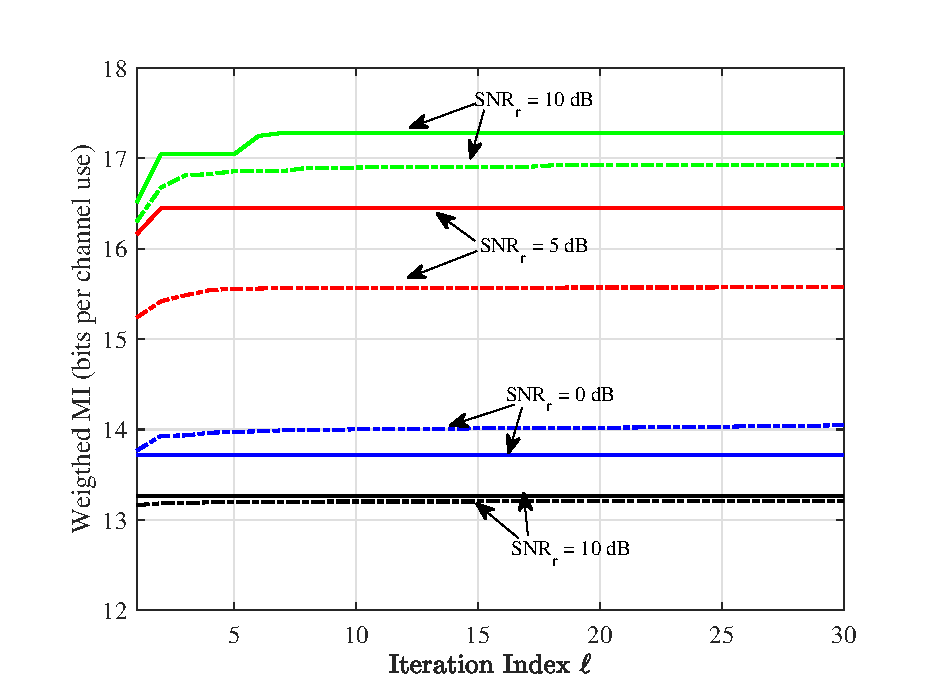
\includegraphics[width=1\columnwidth]{tsp_convergence_snr_nolegend.eps}
	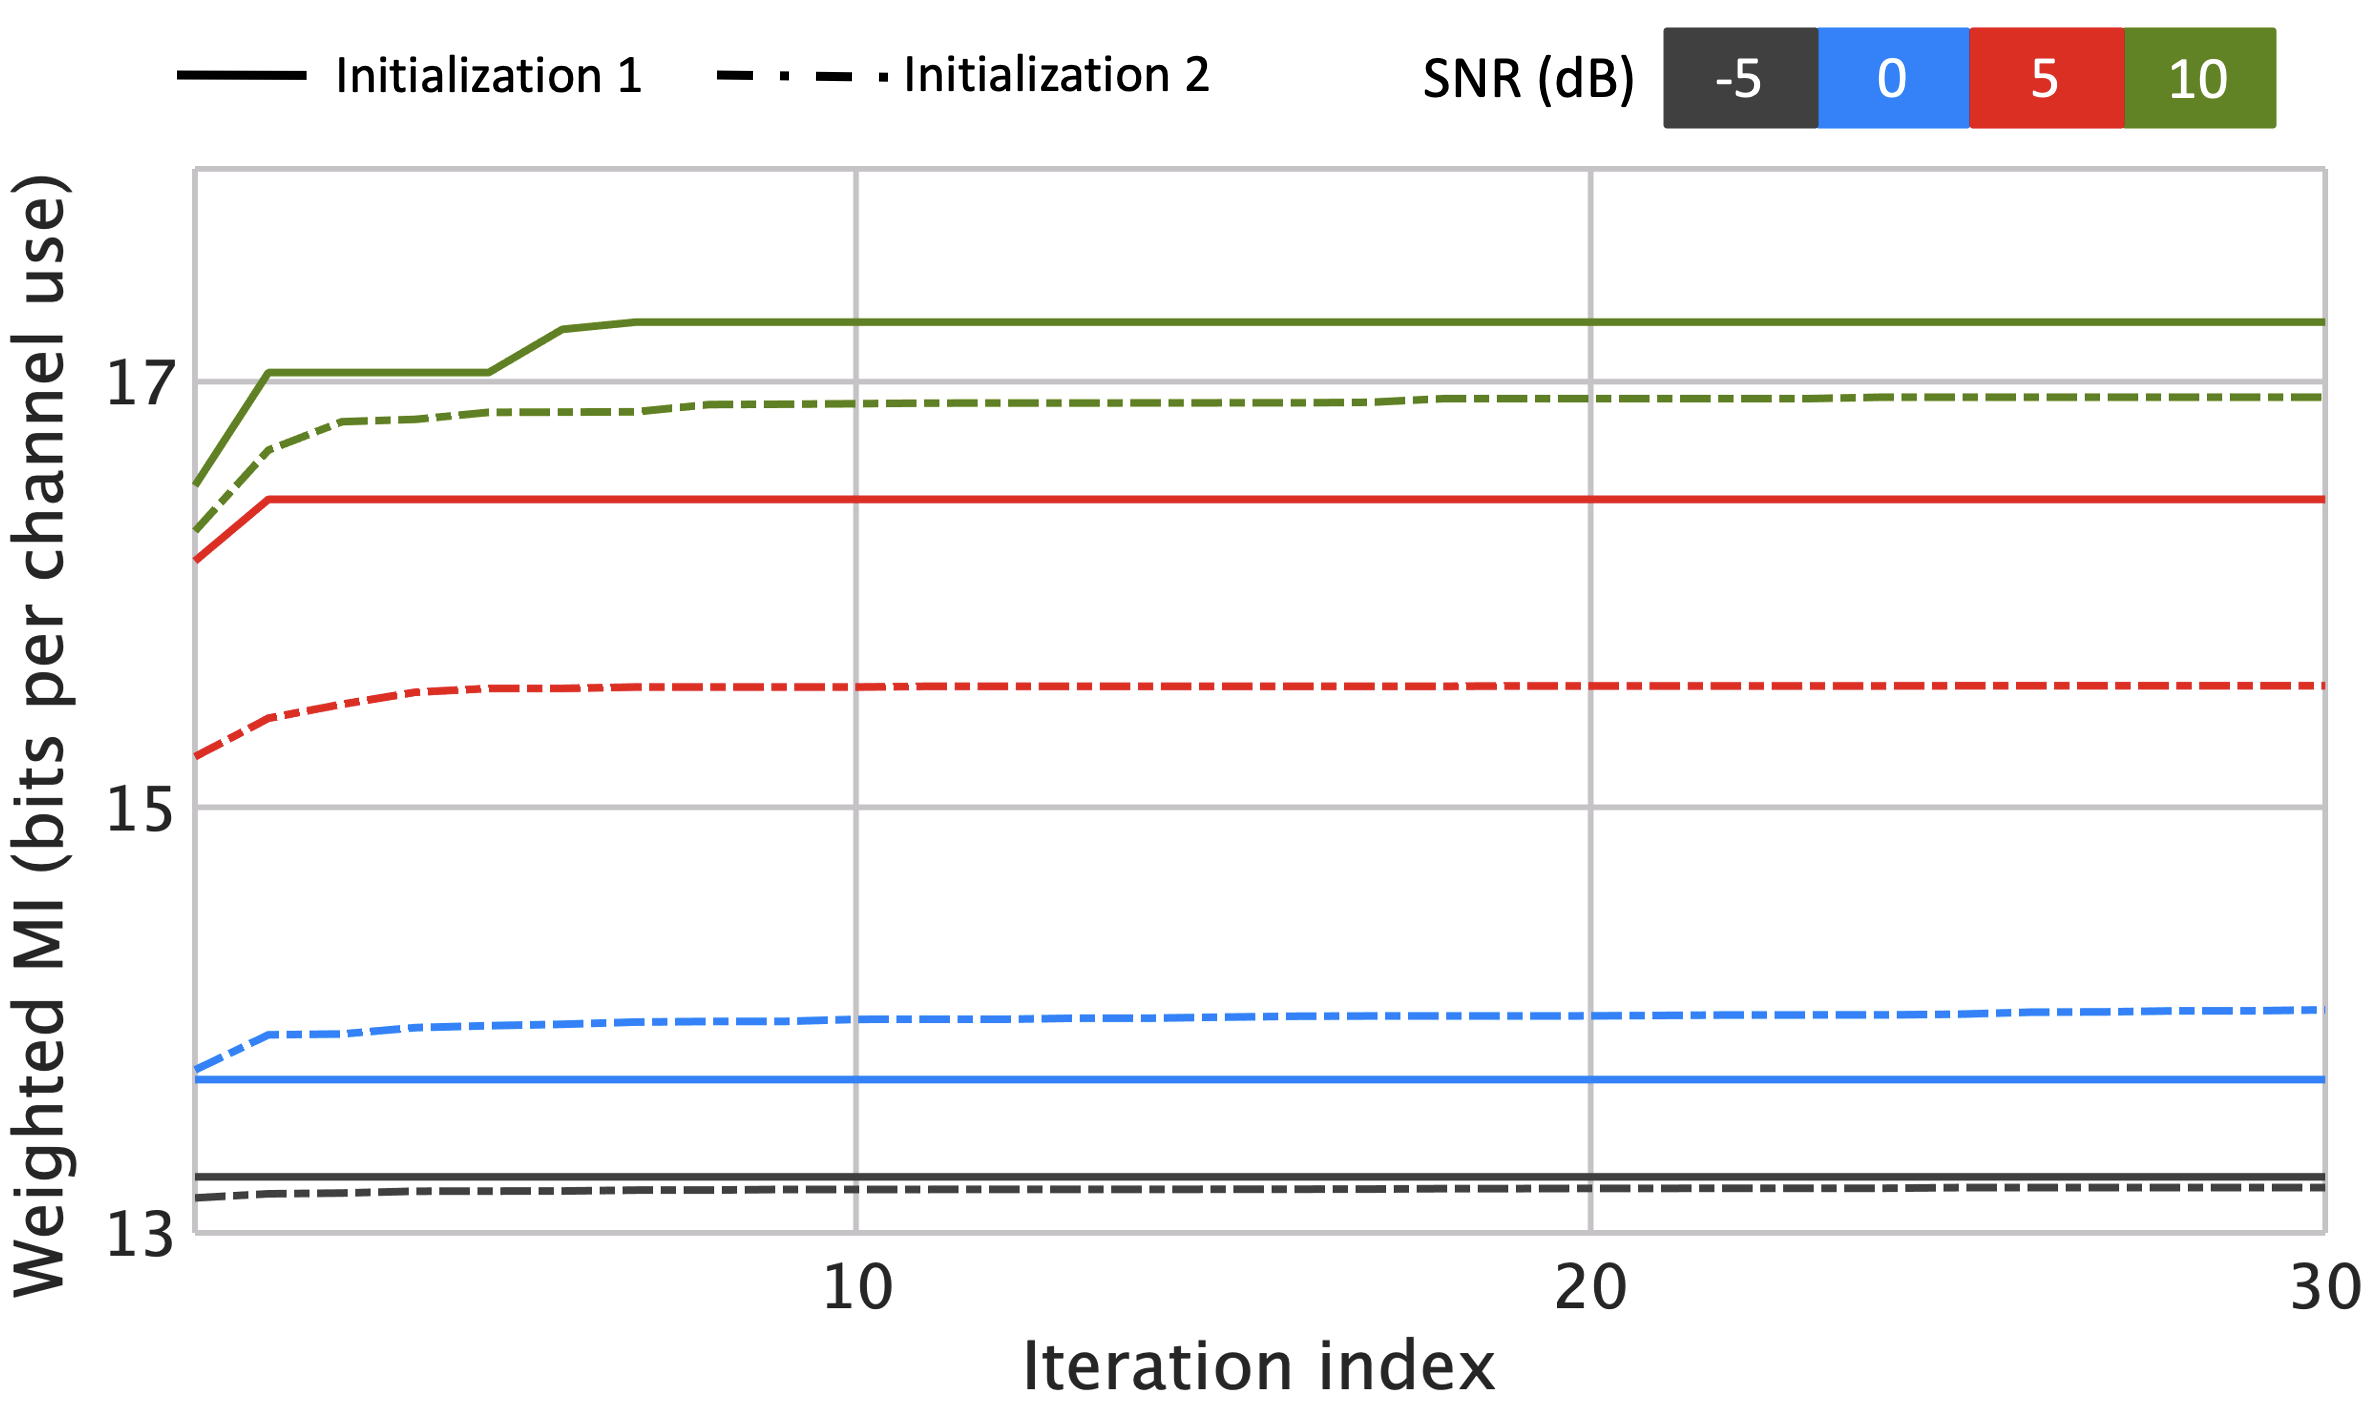
\includegraphics[width=1.0\columnwidth]{tsp_convergence_v03.png}
	%\vspace{-pt}
	\caption{Convergence behaviors of Algorithm $\ref{Alternating_sum}$ with two initialization methods and multiple $\mathrm{SNR}_\textrm{r}$ values.}
	\label{fig:convergence}
	\vspace{-1em}
\end{figure}
\iffalse
\begin{figure}[!ht]
\centering
\subfloat[$\mathrm{SNR}_\textrm{r}=0\textrm{ dB}$ ]{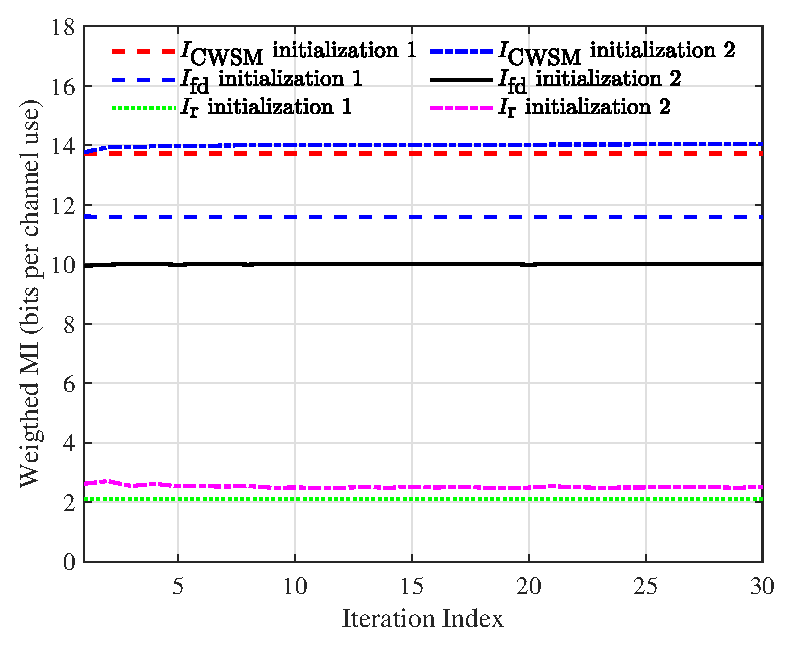
\includegraphics[width=0.45\linewidth]{tsp_convergence_0dB.eps}
\label{fig: con_0dB}}
\hfil
\subfloat[$\mathrm{SNR}_\textrm{r}=10\textrm{ dB}$]{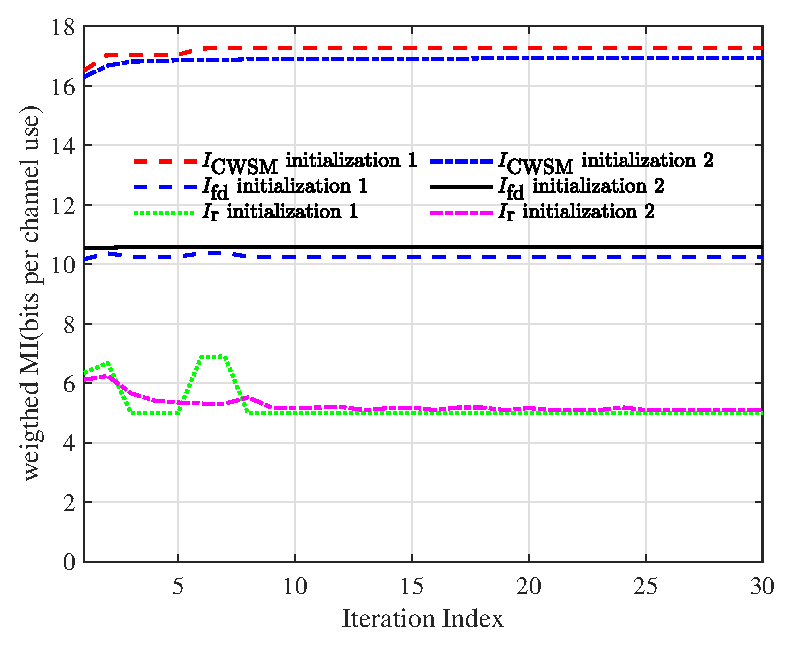
\includegraphics[width=0.45\linewidth]{tsp_convergence_10dB.eps}
\label{fig: con_5dB}}
\caption{Convergence behaviors of Algorithm $\ref{Alternating_sum}$ with two initialization methods}
\label{fig: convergence}
\vspace{-1em}
\end{figure}
\fi
\vspace{-1em}
\subsection{Radar detection performance evaluation}
%-------------------------------------------------------------
\begin{figure}[t]
\vspace{-1em}
\centering
%\subfloat[$\mathrm{P}_{\textrm{d}}$ versus $\nu$ ]{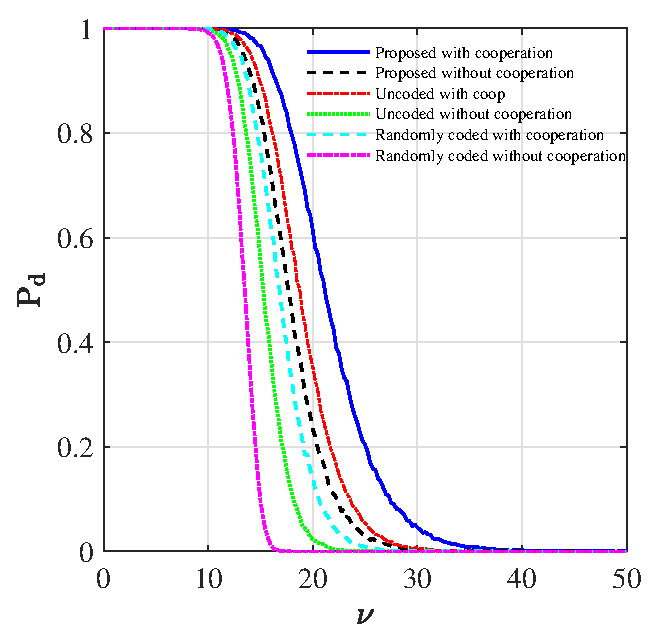
\includegraphics[width=0.48\linewidth]{tsp_pd_vs_vu.eps}
%\label{fig: pd_vs_vu}}
%\hfil
%\subfloat[ROC of the NP detector]{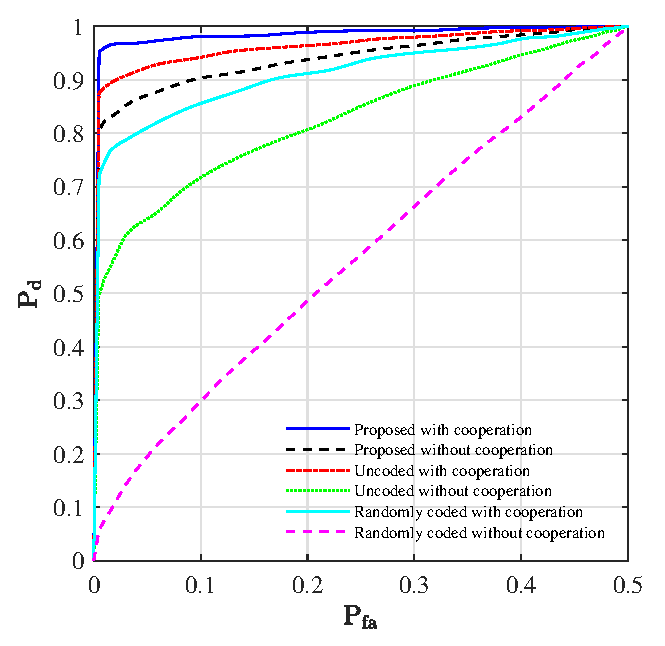
\includegraphics[width=0.48\linewidth]{tsp_ROC.eps}
%\label{fig: roc}}
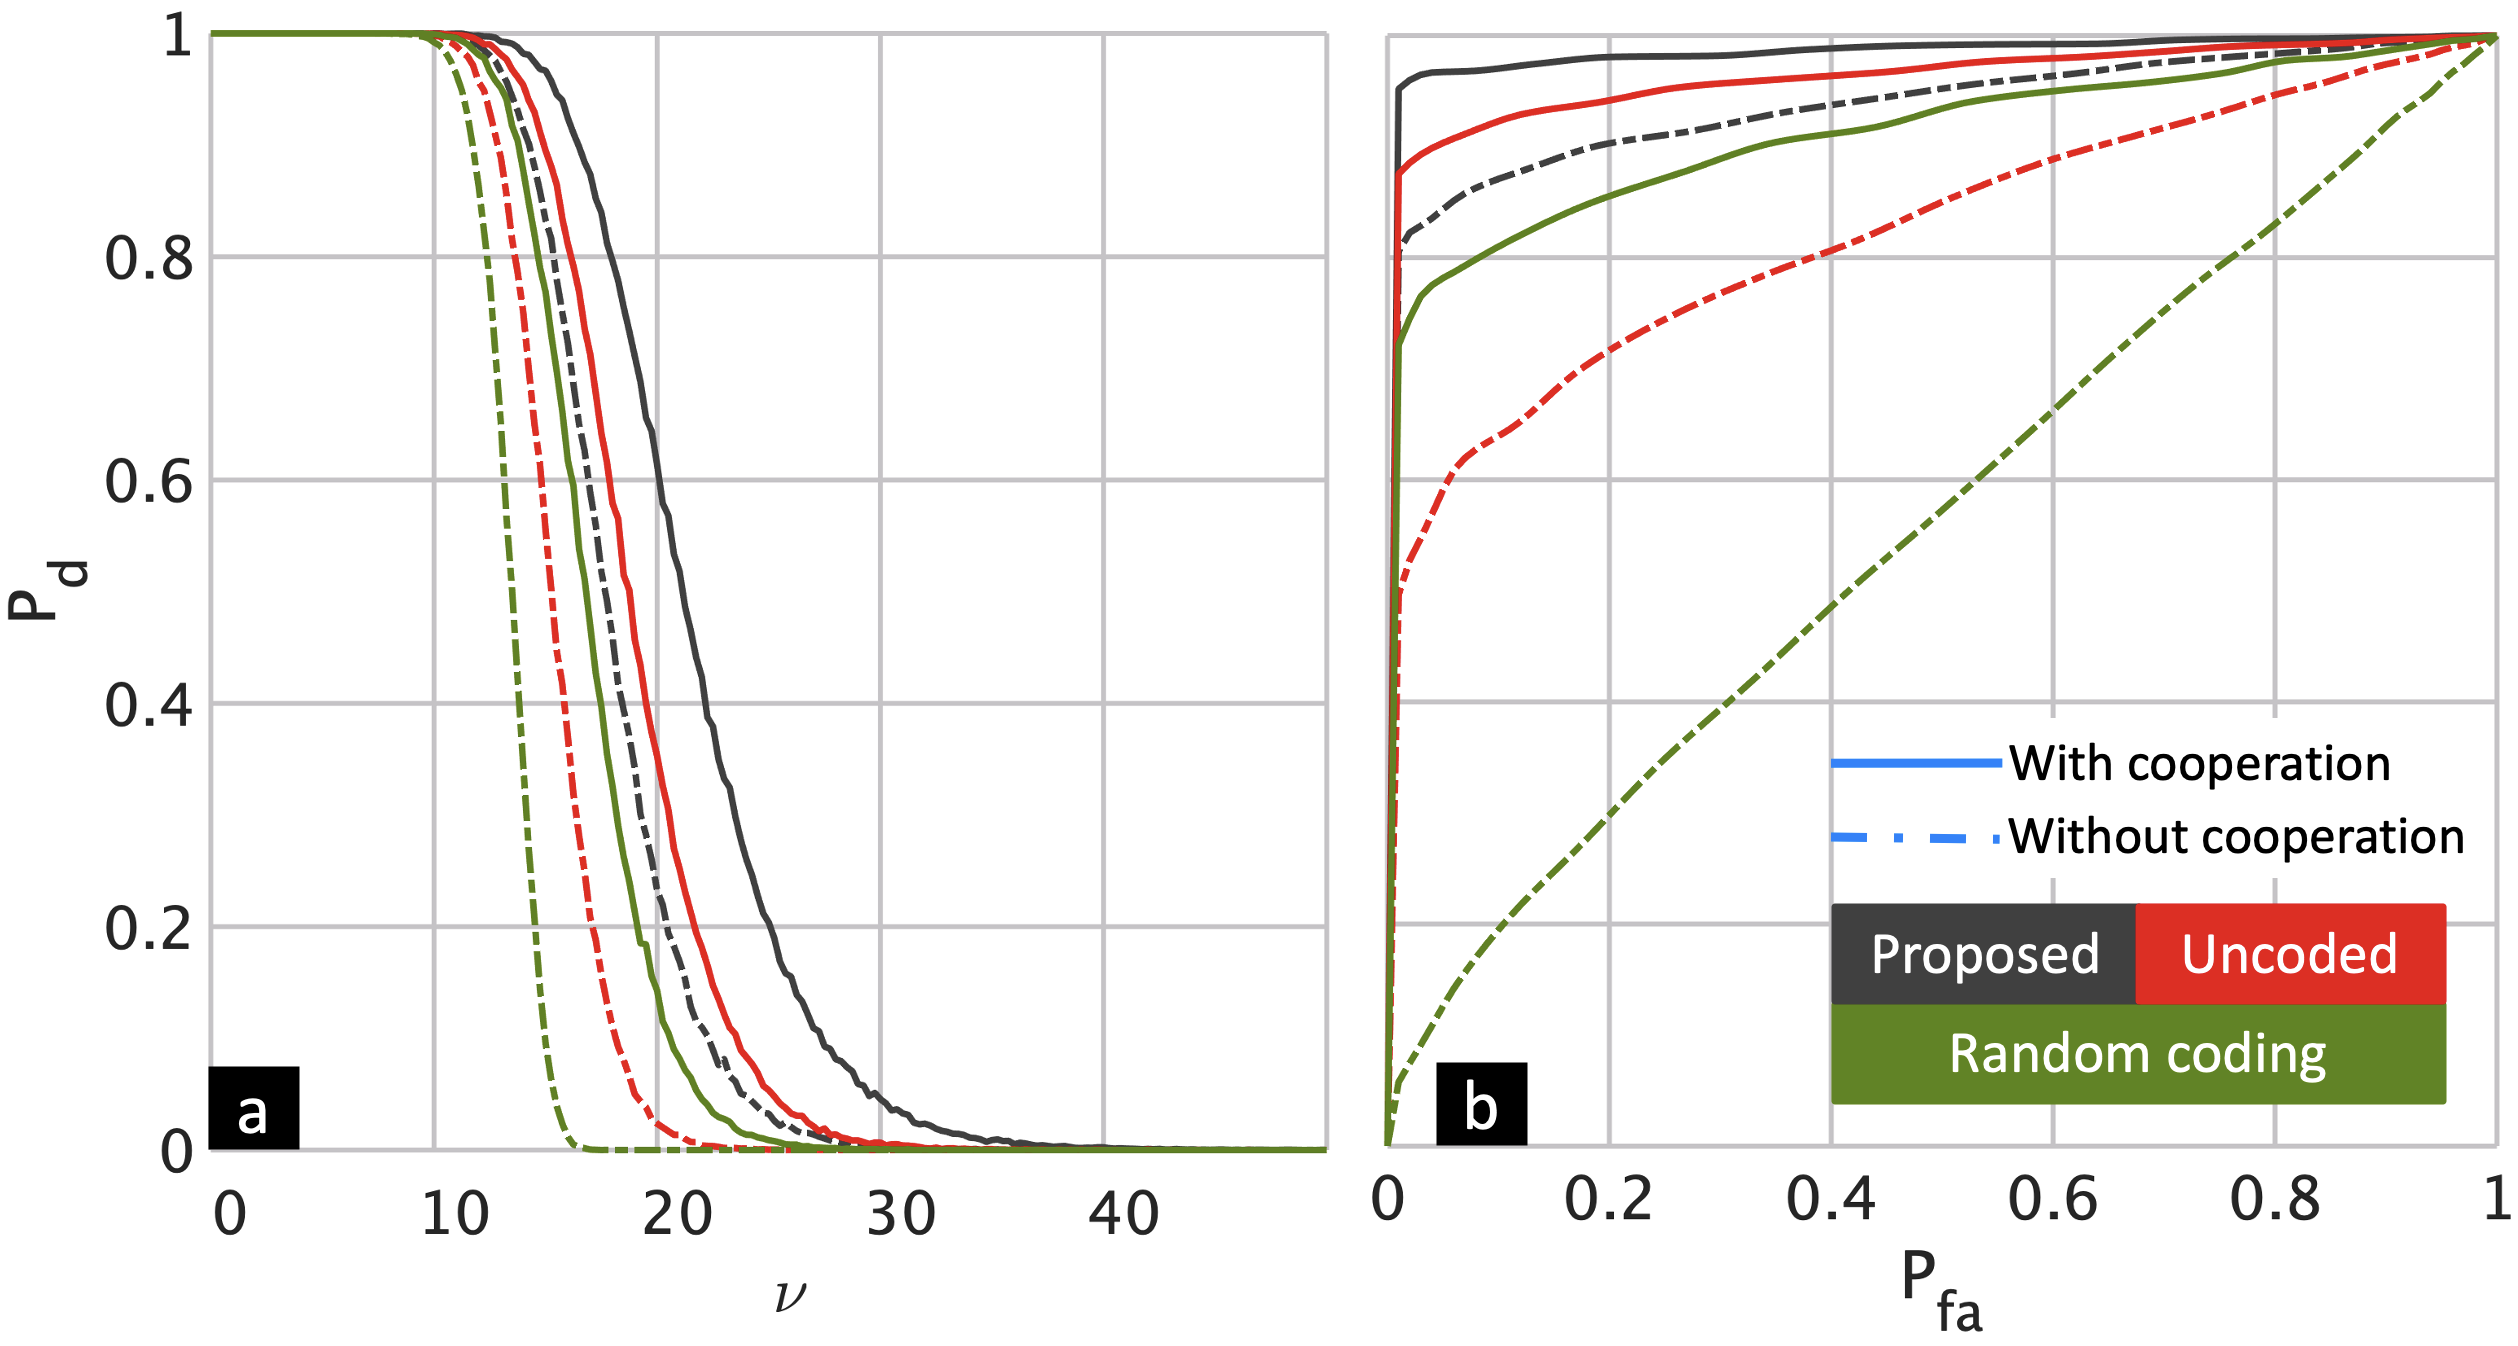
\includegraphics[width=1.0\columnwidth]{NPdetector.png}
\caption{Target detection performance of the coexisting system compared with other radar codes and cooperation schemes using the NP detector. (a) $\mathrm{P}_{\textrm{d}}$ versus $\nu$ (b) ROC of the NP detector.}
\label{fig: NPdetector}
\vspace{-1em}
\end{figure}
%-------------------------------------------------------------
In this experiment, we study the detection performance of the statistical MIMO radar using the designed code matrix $\mathbf{A}$ based on a Newman-Pearson (NP) detector. A target detection problem is formulated as a binary hypothesis test in $\paren{\ref{eq: hypothesis}}$ as
\par\noindent\small
\begin{equation}
\label{eq: hypothesis}
\begin{cases}
\mathrm{H}_{\mathrm{0}}: & \mathbf{y}_{\textrm{r}} = \mathbf{y}_{\textrm{cr}}+\mathbf{y}_{\textrm{Bmr}}+\mathbf{y}_{\textrm{Ur}}+\mathbf{z}_{\textrm{r}}
\\
\mathrm{H}_{\mathrm{1}}: & \mathbf{y}_{\mathrm{r}} = \mathbf{y}_{\textrm{tr}}+ \mathbf{y}_{\textrm{cr}}+\mathbf{y}_{\textrm{Bmr}}+\mathbf{y}_{\textrm{Ur}}+\mathbf{z}_{\textrm{r}}
\end{cases}
\end{equation}
%$\mathbf{y}_{\textrm{cr}}=\bracket{\mathbf{y}^\top_{\textrm{c},1};\cdots;\mathbf{y}^\top_{\textrm{c},\mathit{N}\rr}}^\top$, $\mathbf{y}_{\textrm{Bmr}}=\bracket{\mathbf{y}^\top_{\textrm{Bm},1};\cdots;\mathbf{y}^\top_{\textrm{Bm},\mathit{N}\rr}}^\top$, $\mathbf{y}_{\textrm{Ur}}=\bracket{\mathbf{y}^\top_{\textrm{Ur},1};\cdots;\mathbf{y}^\top_{\textrm{Ur},\mathit{N}\rr}}^\top$, $\mathbf{z}_{\textrm{r}}=\bracket{\mathbf{z}^\top_{\textrm{r},1};\cdots;\mathbf{z}^\top_{\textrm{r},\mathit{N}\rr}}^\to p$, and $\mathbf{y}_{\textrm{tr}}=\bracket{\mathbf{y}^\top_{\textrm{tr},1};\cdots;\mathbf{y}^\top_{\textrm{tr},\mathit{N}\rr}}^\top$.  whose CMs can be written as  $\mathbf{R}_{\mathrm{t}}=\oplus_{n\rr=1}^{\mathit{N}\rr}\mathbf{R}_{\textrm{t},n\rr}$, $\mathbf{R}_{\mathrm{c}}=\oplus_{n\rr}^{\mathit{N}\rr}$
%Notice that the $\mathbf{y}_{\mathrm{c},\textrm{r}}$, $\mathbf{y}_{\mathrm{Bm}}$, $\mathbf{y}_{\mathrm{U}}$, and $\mathbf{z}$ are all zero mean Gaussian random vectors  with CMs being $\mathbf{R}_{\mathrm{t}}=\oplus_{n\rr=1}^{\mathit{N}\rr}\mathbf{R}_{\textrm{t},n\rr}$, $\mathbf{R}_{\mathrm{c}}=\oplus_{n\rr}^{\mathit{N}\rr}$. 
\iffalse
\begin{equation}
\label{eq: hypothesis}
\begin{cases}
\mathrm{H}_{\mathrm{0}}: & \mathbf{y}_{\mathrm{r}} = \mathbf{y}^\textrm{r}_{\textrm{in}}
\\
\mathrm{H}_{\mathrm{1}}: & \mathbf{y}_{\mathrm{r}} = \mathbf{y}_{\mathrm{t}}+ \mathbf{y}^\textrm{r}_{\textrm{in}},
\end{cases}
\end{equation}
where $\mathbf{y}_{\mathrm{r}}=\bracket{\mathbf{y}^\top_{\textrm{r},1};\cdots;\mathbf{y}^\top_{\textrm{r},\mathit{N}\rr}}^\top$ and $\mathbf{y}^\textrm{r}_{\textrm{in}}=\bracket{\paren{\mathbf{y}^{\textrm{r}}_{\textrm{in},n\rr}}^\top;\cdots;\paren{\mathbf{y}^{\textrm{r}}_{\textrm{in},\mathit{N}\rr}}^\top}^\top$,
\fi
where $\mathbf{y}_{\mathrm{r}}=\bracket{\mathbf{y}^\top_{\textrm{r},1};\cdots;\mathbf{y}^\top_{\textrm{r},\mathit{N}\rr}}^\top$ and $\mathbf{y}_{\textrm{tr}}=\bracket{\mathbf{y}^\top_{\textrm{tr},1};\cdots;\mathbf{y}^\top_{\textrm{tr},\mathit{N}\rr}}^\top$. We denote $\mathbf{y}^\textrm{r}_{\textrm{in}}\triangleq\mathbf{y}_{\textrm{cr}}+\mathbf{y}_{\textrm{Bmr}}+\mathbf{y}_{\textrm{Ur}}+\mathbf{z}_{\textrm{r}}=\bracket{\paren{\mathbf{y}^{\textrm{r}}_{\textrm{in},n\rr}}^\top;\cdots;\paren{\mathbf{y}^{\textrm{r}}_{\textrm{in},\mathit{N}\rr}}^\top}^\top$ and its CM $\mathbf{R}_{\textrm{in}}=\oplus\mathbf{R}_{\textrm{in},n\rr}$. We continue to define $\overline{\mathbf{y}}_{\textrm{r},n\rr} = \mathbf{R}^{-\sfrac{1}{2}}_{\textrm{in},n\rr}\mathbf{y}_{\textrm{r},n\rr}$ and this results in the CM of $\overline{\mathbf{y}}_{\textrm{r},n\rr}$ as $\mathbf{G}_{n\rr}=\mathbf{R}^{-\sfrac{1}{2}}_{\textrm{in},n\rr}\mathbf{R}_{\textrm{t},n\rr}\mathbf{R}^{-\sfrac{1}{2}}_{\textrm{in},n\rr}$, we can rewrite the hypothesis test problem as  \par\noindent\small
%If $\mathbf{M}_{n\rr}\triangleq\mathbf{R}_{\textrm{in},n\rr }$ and  , the test problem can be rewritten as 
\begin{equation}
\begin{cases}
\mathrm{H}_{\mathrm{0}}: & \overline{\mathbf{y}}_{\mathrm{r}}\sim\mathcal{CN}\paren{\mathbf{0},\mathbf{I}}
\\
\mathrm{H}_{\mathrm{1}}: & \overline{\mathbf{y}}_{\mathrm{r}}\sim\mathcal{CN}\paren{\mathbf{0},\mathbf{I}+\mathbf{G}}
\end{cases}
\end{equation}\normalsize
where the block diagonal matrix $\mathbf{G}=\oplus_{n\rr=1}^{\mathit{N}\rr}\mathbf{G}_{n\rr}$. The eigendecomposition of $\mathbf{G}_{n\rr}$ is expressed as $\mathbf{G}_{n\rr}=\mathbf{V}_{n\rr}\mathbf{\Lambda}_{n\rr}\mathbf{V}^\dagger_{n\rr}$, where the columns of $\mathbf{V}_{n\rr}$ and the diagonal entries of $\mathbf{\Lambda}_{n\rr}\triangleq\diag\bracket{\delta_{1,n\rr},\cdots,\delta_{\mathit{K},n\rr}}$ contain the eigenvectors and eigenvalues of $\mathbf{G}_{n\rr}$, respectively, where $\delta_{k,n\rr}$ is the $\ith{k}$ eigenvalue of $\mathbf{G}_{n\rr}$. With the Woodbury matrix identity and the eigendecomposition of $\mathbf{G}_{n\rr}$, the test statistic can be written as\par\noindent\small
\begin{flalign}
T\paren{\overline{\mathbf{y}}}&=\sum_{n\rr=1}^{\mathit{N}\rr}T\paren{\overline{\mathbf{y}}_{\textrm{r},n\rr}}=\sum_{n\rr=1}^{\mathit{N}\rr}\overline{\mathbf{y}}^\dagger_{\textrm{r},n\rr}\paren{\mathbf{I}-\paren{\mathbf{G}_{n\rr}+\mathbf{I}}^{-1}}\overline{\mathbf{y}}_{\textrm{r},n\rr}\nonumber\\
&=\sum_{n\rr=1}^{\mathit{N}\rr}\overline{\mathbf{y}}^\dagger_{\textrm{r},n\rr}\mathbf{V}_{n\rr}\paren{\mathbf{\Lambda}^{-1}+\mathbf{I}}^{-1}\mathbf{V}^\dagger_{n\rr}\overline{\mathbf{y}}_{\textrm{r},n\rr}
\end{flalign}\normalsize
If we denote $\widehat{\mathbf{y}}_{\textrm{r},n\rr}=\mathbf{V}^\dagger_{n\rr}\overline{\mathbf{y}}_{\textrm{r},n\rr}=\bracket{\widehat{y}_{n\rr}\bracket{1},\cdots,\widehat{y}_{n\rr}\bracket{\mathit{K}}}$, then the Newman-Pearson (NP) detector can be formulated as\cite{Kay1993detection}
\begin{equation}
\label{eq: NPdetector}
%\sum_{n\rr}^{\mathit{N}\rr}T\paren{\overline{\mathbf{y}}_{\textrm{r},n\rr}}
T\paren{\overline{\mathbf{y}}}=\sum_{n\rr=1}^{\mathit{N}\rr}\sum_{k=1}^{\mathit{K}}\frac{\delta_{k,n\rr}\lvert\widehat{y}_{n\rr}\bracket{k}\rvert^2}{1+\delta_{k,n\rr}}\underset{\mathrm{H}_2}{\overset{\mathrm{H}_1}{\gtrless}}\nu.
\end{equation}
We utilize a Monte Carlo (MC) simulation to evaluate the probability of detection  and the receiver operating characteristic (ROC) of the NP detector $\paren{\ref{eq: NPdetector}}$\cite{Kay1993detection}. In \figurename{\;\ref{fig: NPdetector}$\paren{\mathrm{a}}$} and \figurename{\;\ref{fig: NPdetector}$\paren{\mathrm{b}}$}, we plotted $\mathrm{P}_{\textrm{d}}$ versus the threshold $\nu$ and the ROC of the NP detector, namely the curve of $\mathrm{P}_{\textrm{d}}$ versus the probability of false alarm $\mathrm{P}_{\textrm{fa}}$, respectively, with different combinations of waveform and cooperation schemes. In our simulation setup, with or without cooperation indicates whether or not the DL signals $\mathbf{y}_{\textrm{Bt},n\rr}$ are incorporated in $\mathbf{y}_{\textrm{t,}n\rr}$ for all $n\rr$. For the $\ith{m\rr}$ radar Tx, the uncoded waveform is referred to as $\mathbf{a}_{m\rr}=\sqrt{\frac{\mathrm{P}_{\textrm{r},m\rr}}{\mathit{K}}}\mathbf{1}_{\mathit{K}}$ and the randomly coded waveform is constructed as $\mathbf{a}_{m\rr}=\sqrt{\frac{\mathrm{P}_{\textrm{r},m\rr}}{\mathit{K}}}\mathbf{u}_{m\rr}$ , where $\braces{\mathbf{u}_{m\rr}}$ is a unitary basis. We respectively generated $5000$ realizations of $\overline{\mathbf{y}}_{\textrm{r}}$ under hypothesis $\mathrm{H}_1$ to estimate $\mathrm{P}_{\textrm{d}}$ and $\mathrm{H}_0$ to estimate $\mathrm{P}_{\textrm{fa}}$ based on $\nu$ for each considered scheme. Both \figurename{\;\ref{fig: NPdetector}$\paren{\mathrm{a}}$} and \figurename{\;\ref{fig: NPdetector}$\paren{\mathrm{b}}$} illustrate that the proposed radar waveform codes outperform the all-one and random coding schemes, and that the cooperation between the radar and BS boosts the radar detection performance. For example in \figurename{\;\ref{fig: NPdetector}$\paren{\mathrm{b}}$}, with $P_{\textrm{fa}}=0.1$, using the radar codes and communications precoders designed by Algorithm \ref{Alternating_sum} with radar-DL cooperation yields an approximately $8\%$ $P_{\textrm{d}}$ improvement compared to the scenario without the cooperation as well as  $6\%$ and $13\%$ gains compared to using the all-one and random codes even with the radar-DL cooperation. We can see even without the cooperation, our algorithm can still allow the MIMO radar to have a competitive detection performance.

\iffalse
\begin{figure}[t]
\centering
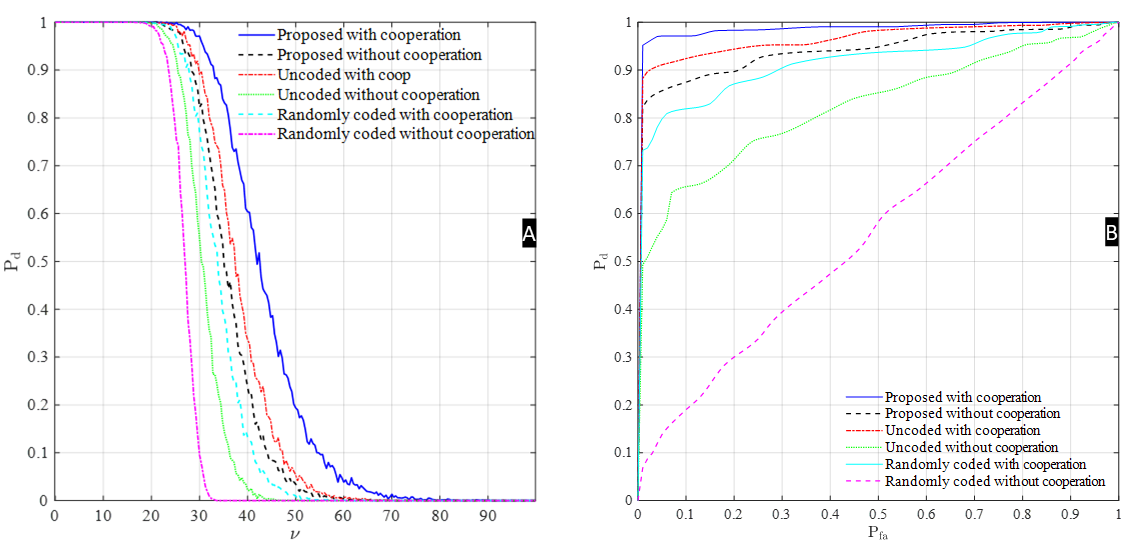
\includegraphics[width=0.45\linewidth]{radar_figures_roc.png}
%\vspace{-14pt}
\caption{$\paren{\textrm{a}}$ $\mathrm{P}_{\textrm{d}}$ versus $\nu$ with different combinations of waveform and cooperation schemes $\paren{\textrm{b}}$ the corresponding ROC of the NP detector}
\label{fig: NPdetector}
\end{figure}
\fi
\vspace{-1em}
\subsection{FD communications performance evaluation}
\label{subsec: fd_comm_eva}
\begin{figure}[t]
\vspace{-1em}
\centering
%\subfloat[Weighted MI versus various number of UL UEs]{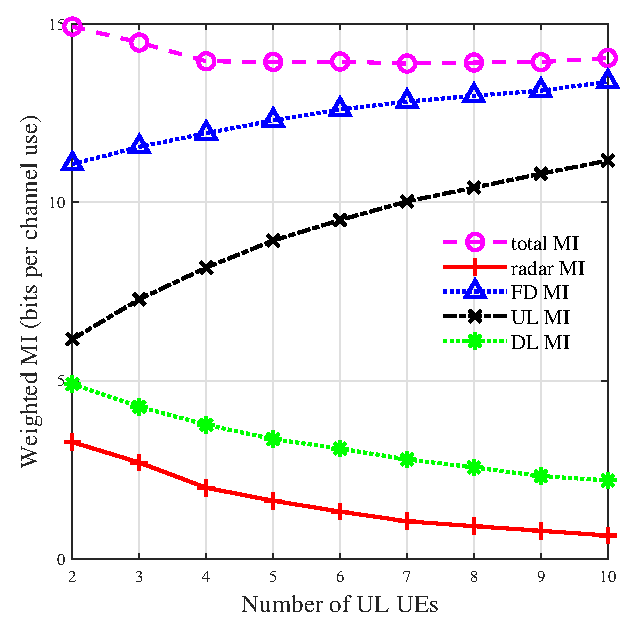
\includegraphics[width=0.48\linewidth]{II.eps}
%\label{fig: UL_UE}}
%\hfil
%\subfloat[Weighted MI versus various number of DL UEs]{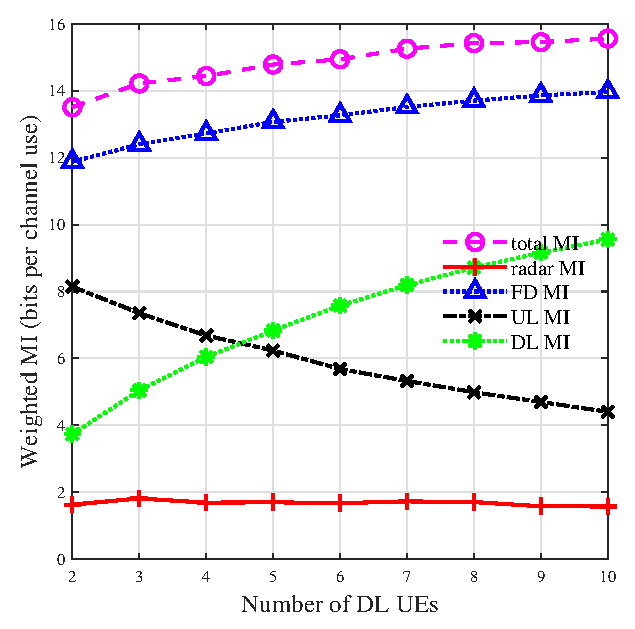
\includegraphics[width=0.48\linewidth]{tsp_DL_UE.eps}
%\label{fig: DL_UE}}
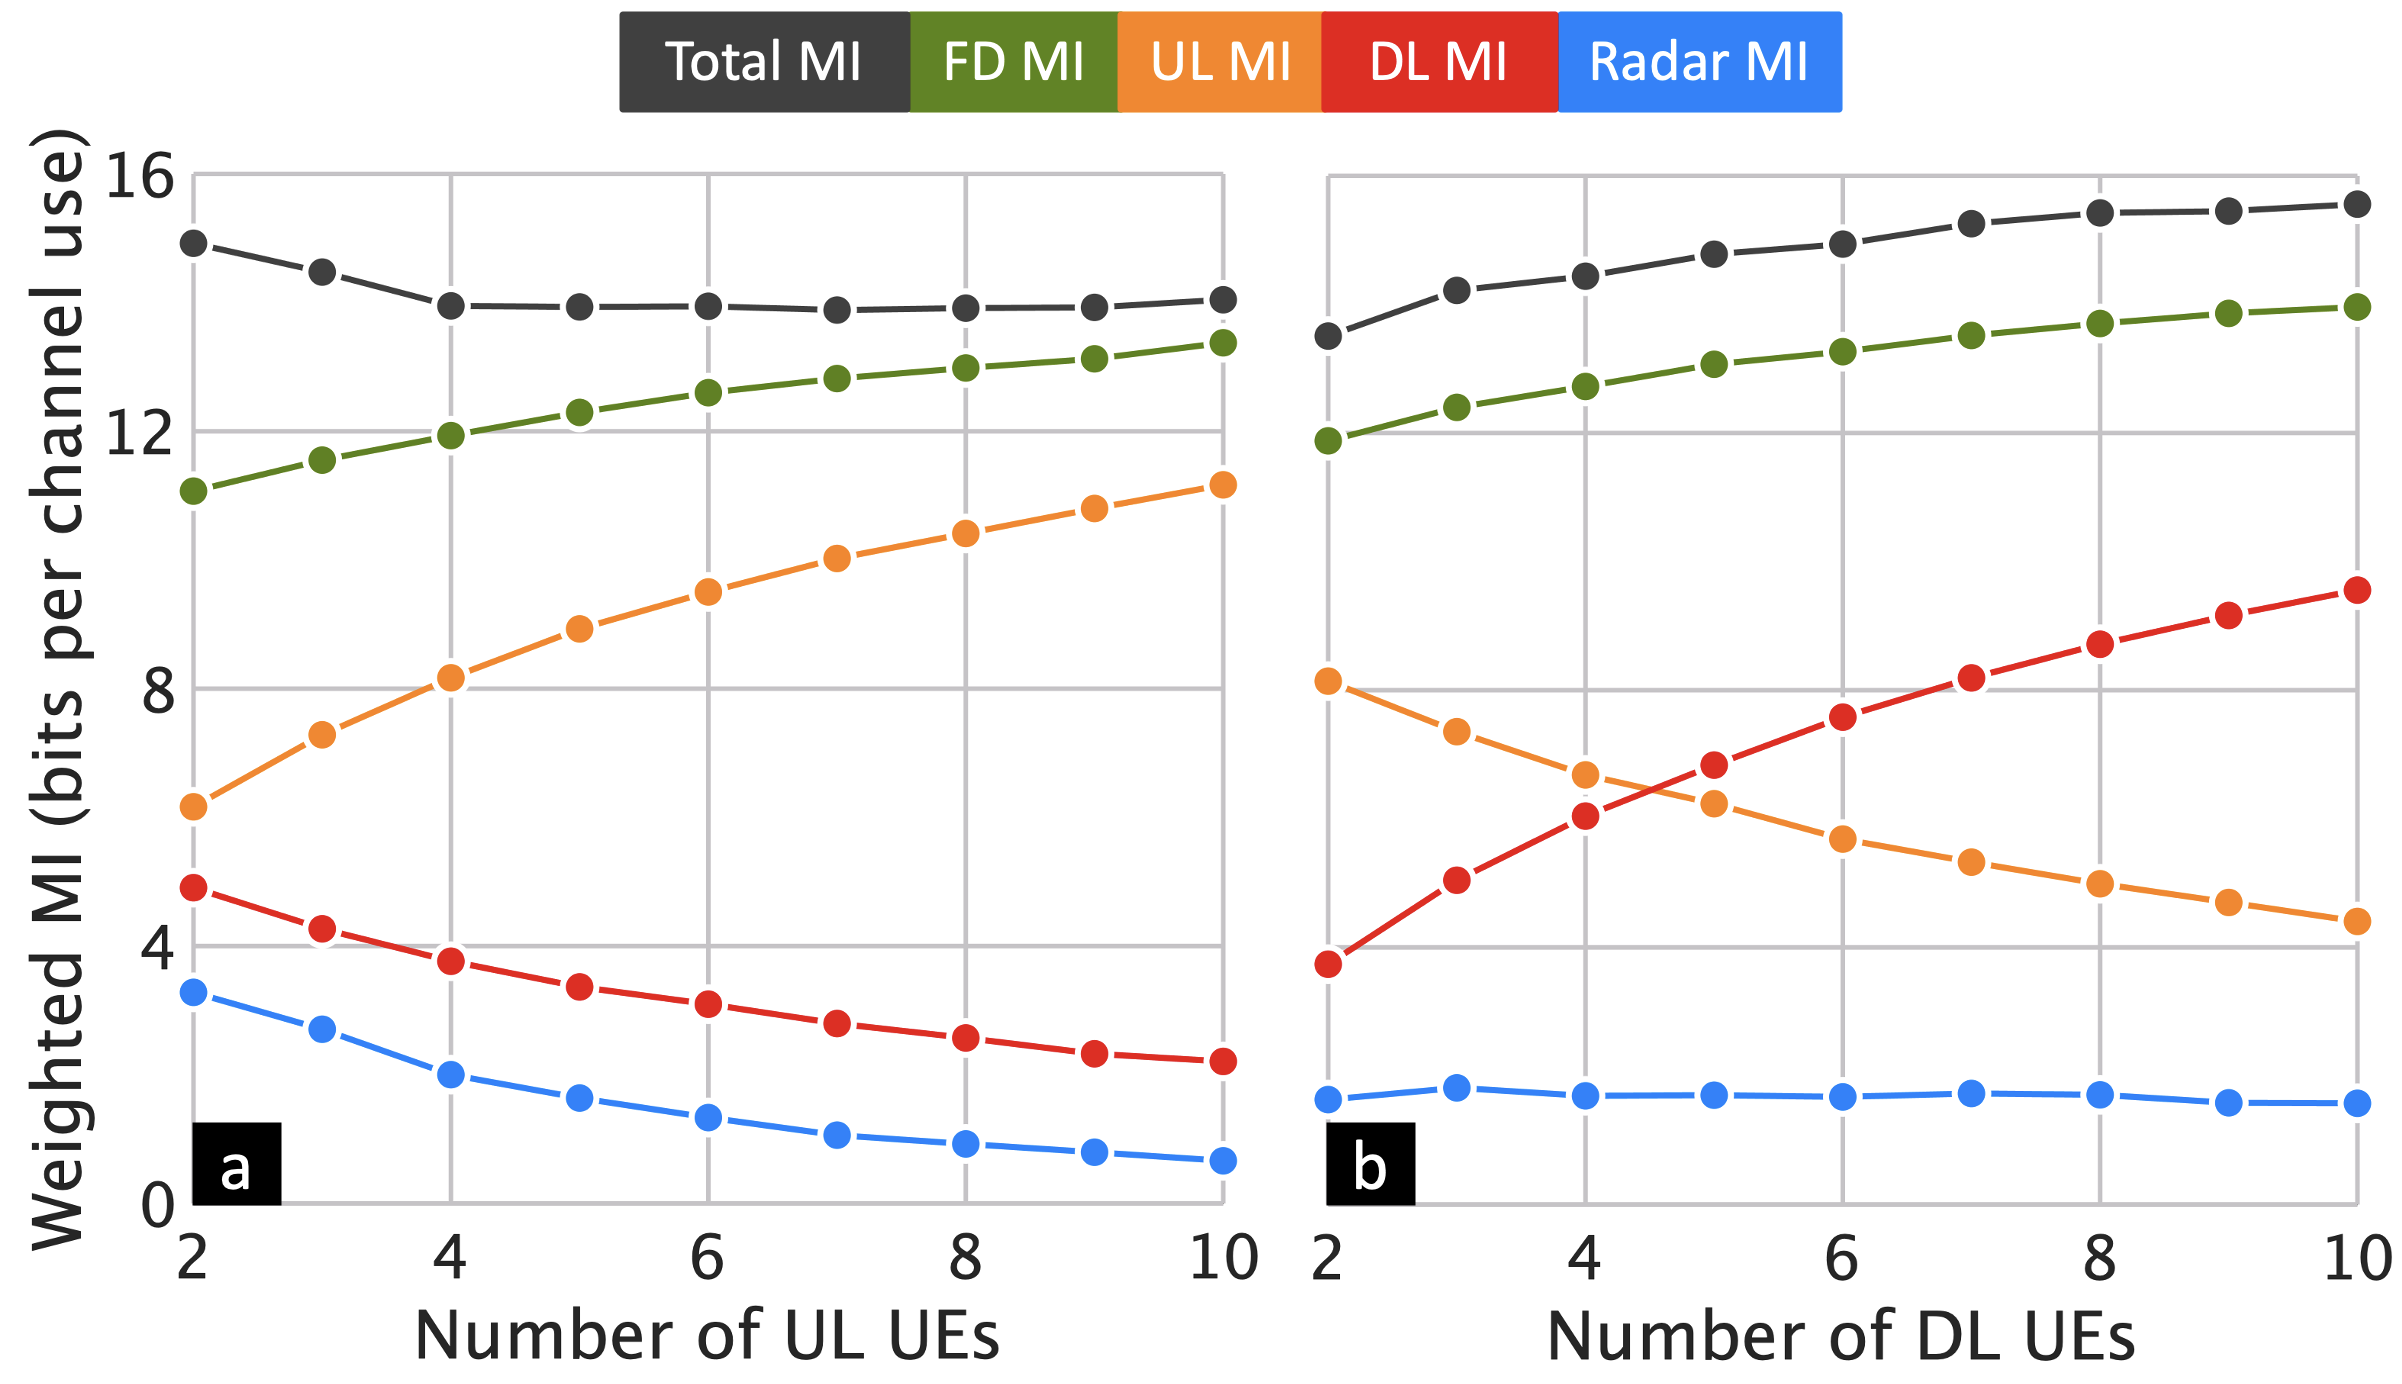
\includegraphics[width=0.9\columnwidth]{fd_UE.png}
\caption{Performance of the coexisting system evaluation compared with various numbers of (a) UL and (b) DL UEs.}
\label{fig:fd_UE}
\vspace{-1em}
\end{figure}
%-------------------------------------------------------------
This experiment explores the relationship between the system performance versus the numbers of communications UEs. In \figurename{\ref{fig:fd_UE}}a and \figurename{\ref{fig:fd_UE}}b, we depicted $\mathit{I}_{\textrm{U}}\triangleq\sum_{k}\sum_{i}\alpha^\textrm{u}_i\mathit{I}_{\textrm{u},i}\bracket{k}$ or the weighted UL MI, $\mathit{I}_{\textrm{D}}\triangleq\sum_{k}\sum_{j}\alpha^\textrm{d}_j\mathit{I}_{\textrm{d},j}\bracket{k}$ or the weighted DL MI, $\mathit{I}_{\textrm{R}}\triangleq\alpha^\textrm{r}_{n\rr}\sum_{n\rr}\mathit{I}_{\textrm{r},n\rr}\bracket{k}$ or the weighted DL MI, the total weighted FD MI as well as $\mathit{I}_{\textrm{CWSM}}$ versus various numbers of UL UEs and DL UEs, respectively. We also assume UL and DL power levels are  $\mathrm{P}_{\textrm{u}}=I$ and $\mathrm{P}_{\textrm{d}}=J$. As the number of UL UEs 
increases from $\mathit{I}=2$ to $\mathit{I}=10$ and the number of DL UEs is fixed at $\mathit{J}=2$, the performances of DL UEs and radar Rxs deteriorate due to the increasing UL interference. On the other hand, the performance of the UL drops while that of the MIMO radar remains relatively stable as the number of DL UEs expands from $\mathit{J}=2$ to $\mathit{J}=10$ with $\mathit{I}=2$. We observe that the total system performance measure  $\mathbf{I}_{\textrm{CWSM}}$ is enhanced with a higher DL power due to the radar-DL cooperation whereas $\mathbf{I}_{\textrm{CWSM}}$ declines with a greater UL power level. 

\vspace{-1em}
\subsection{Joint radar and communications performance evaluation}
%-------------------------------------------------------------
\begin{figure}[t]
	\centering
	%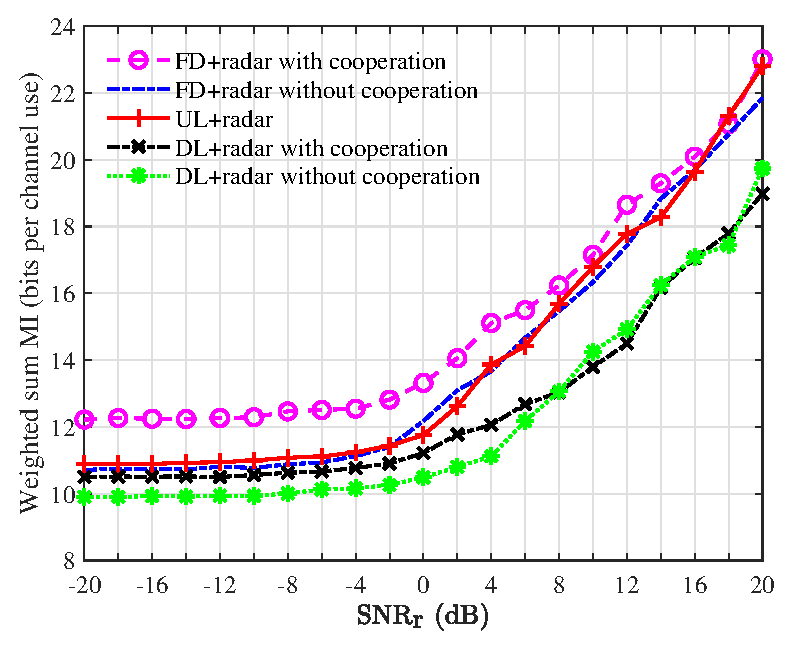
\includegraphics[width=1\columnwidth]{fd_vs_hd.eps}
	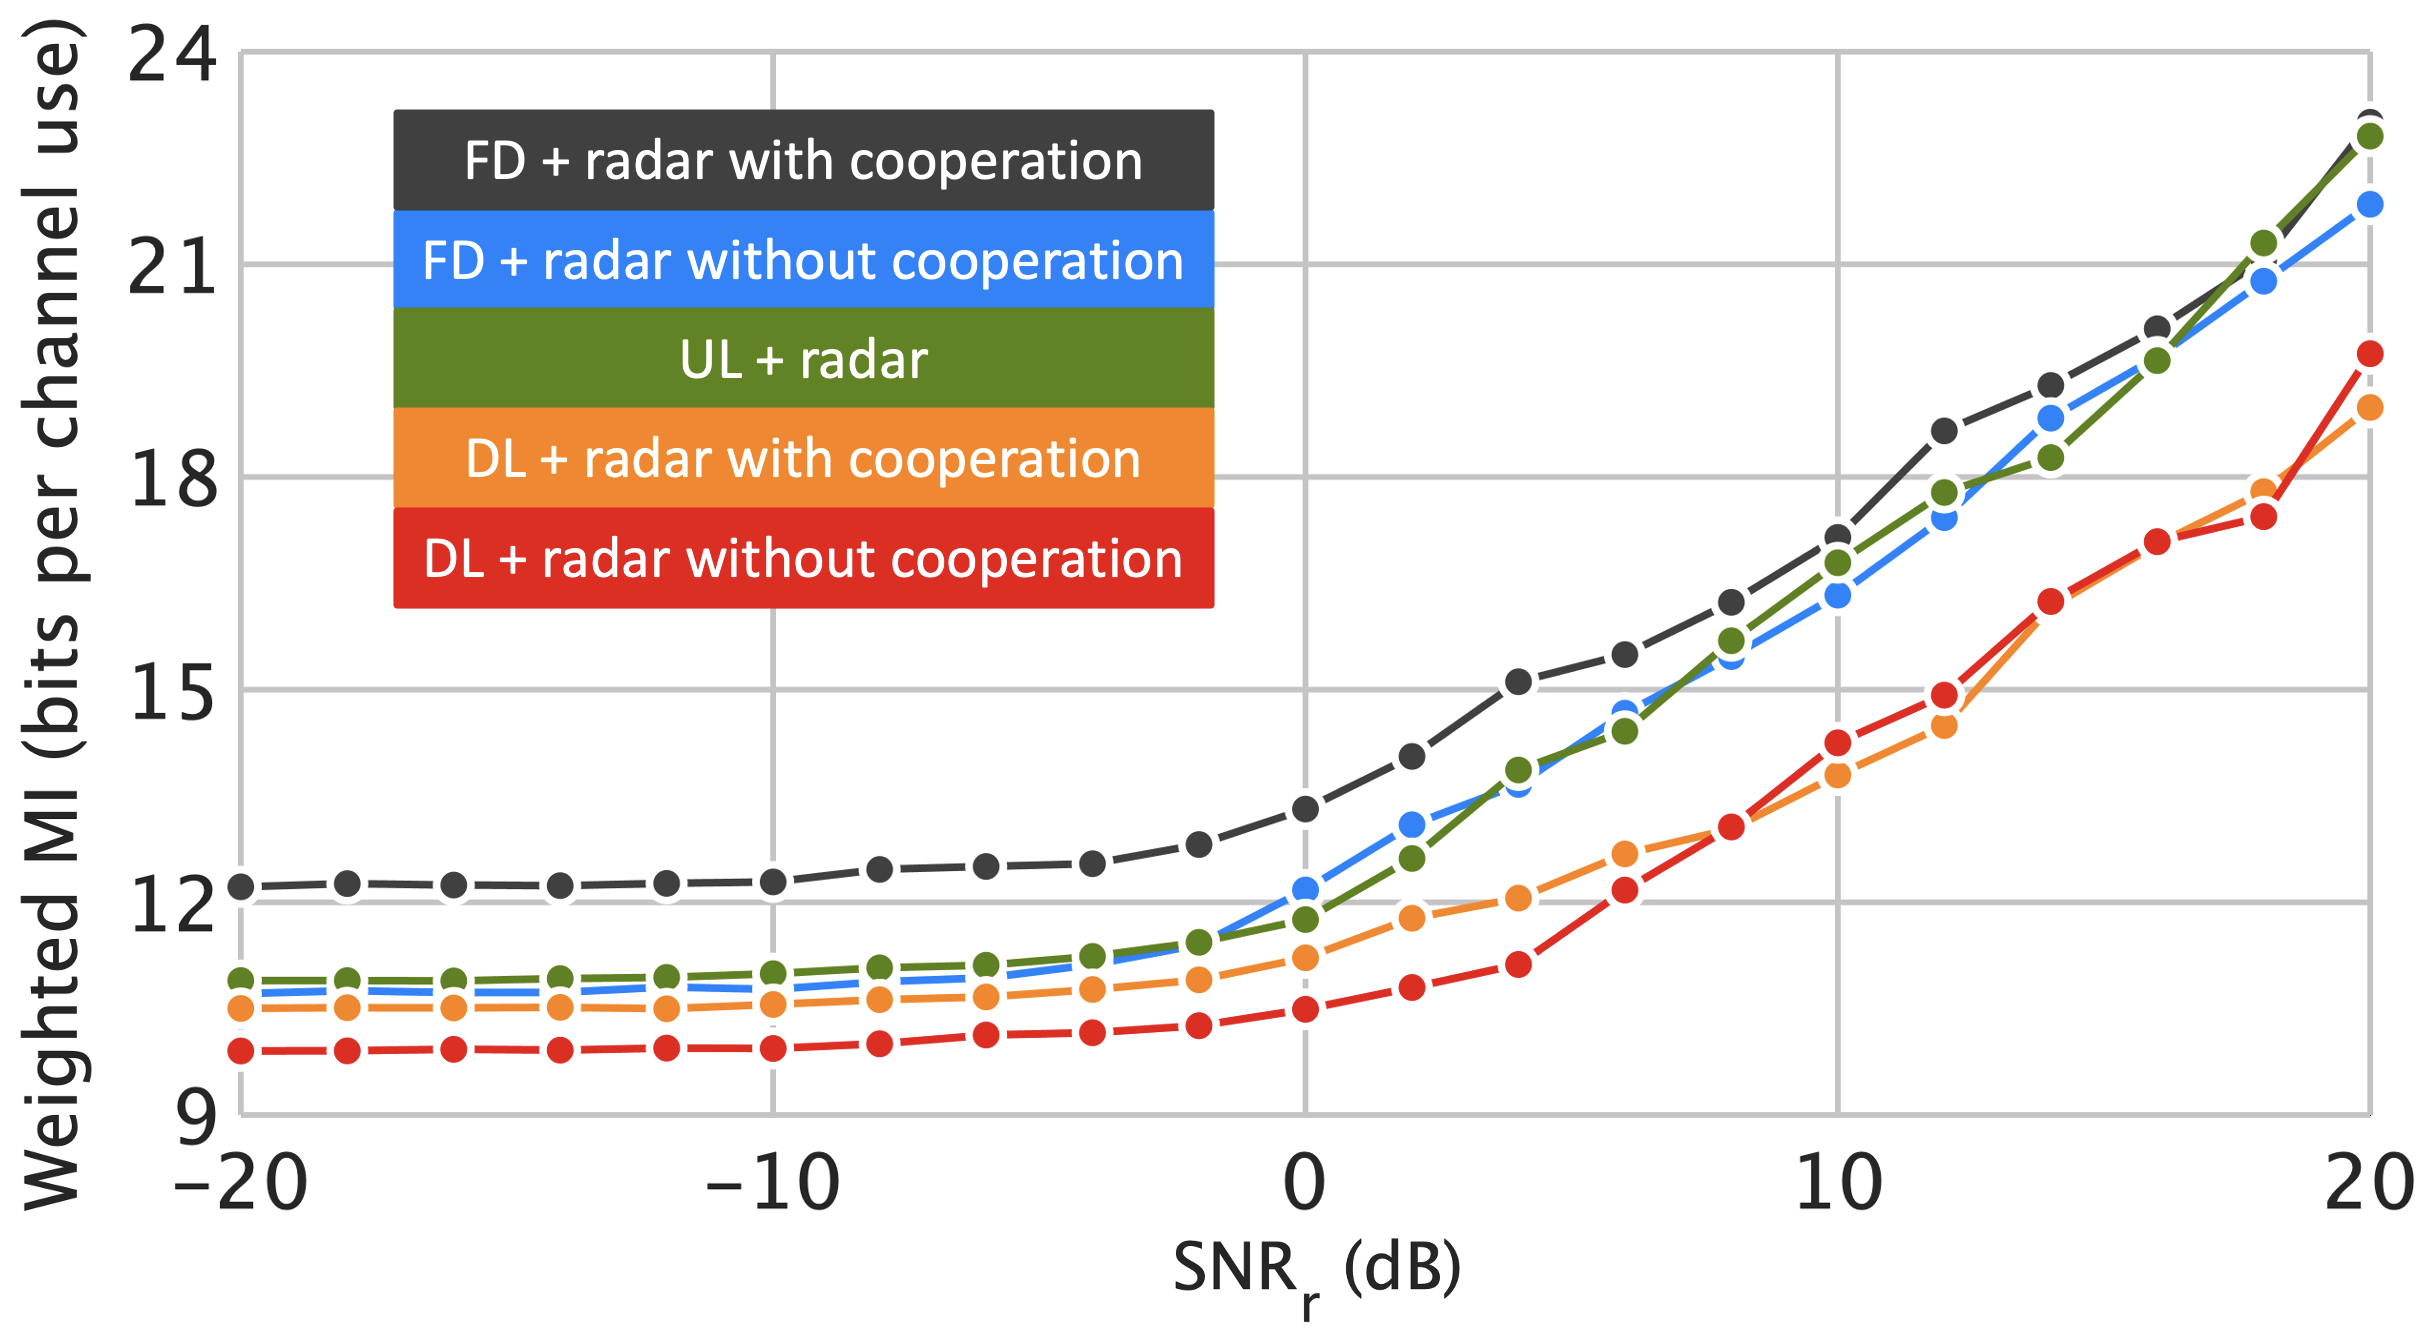
\includegraphics[width=1.0\columnwidth]{fd_vs_hd_v03.png}
	%\vspace{-pt}
	\caption{Evaluation of the MU-MIMO communications with different transmission schemes under various radar SNRs}
	\label{fig:fd_vs_hd}
	\vspace{-1em}
\end{figure}
%-------------------------------------------------------------
\begin{figure}[t]
\centering
%\subfloat[System performance vs UL SNRs]{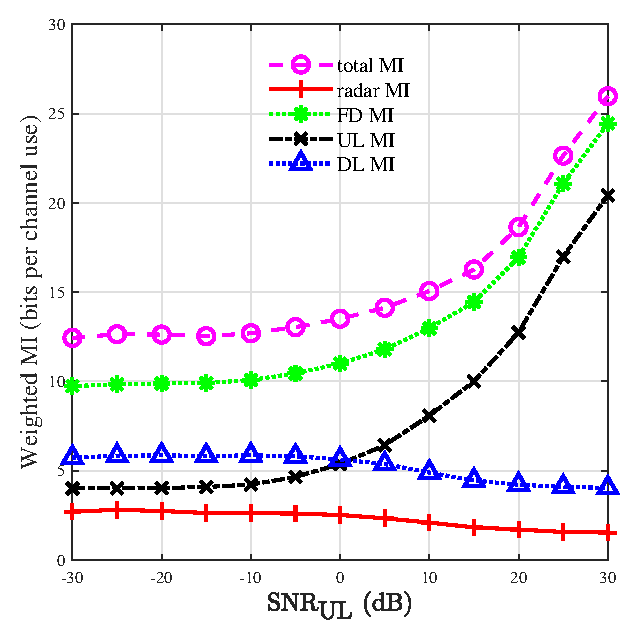
\includegraphics[width=0.48\columnwidth]{UL_SNR_sweep.eps}
%\label{fig: UL_SNR}}
%\hfil
%\subfloat[System performance vs CNR]{\includegraphics[width=0.48\columnwidth]{CNR_sweep.eps}
%\label{fig: CNR}}
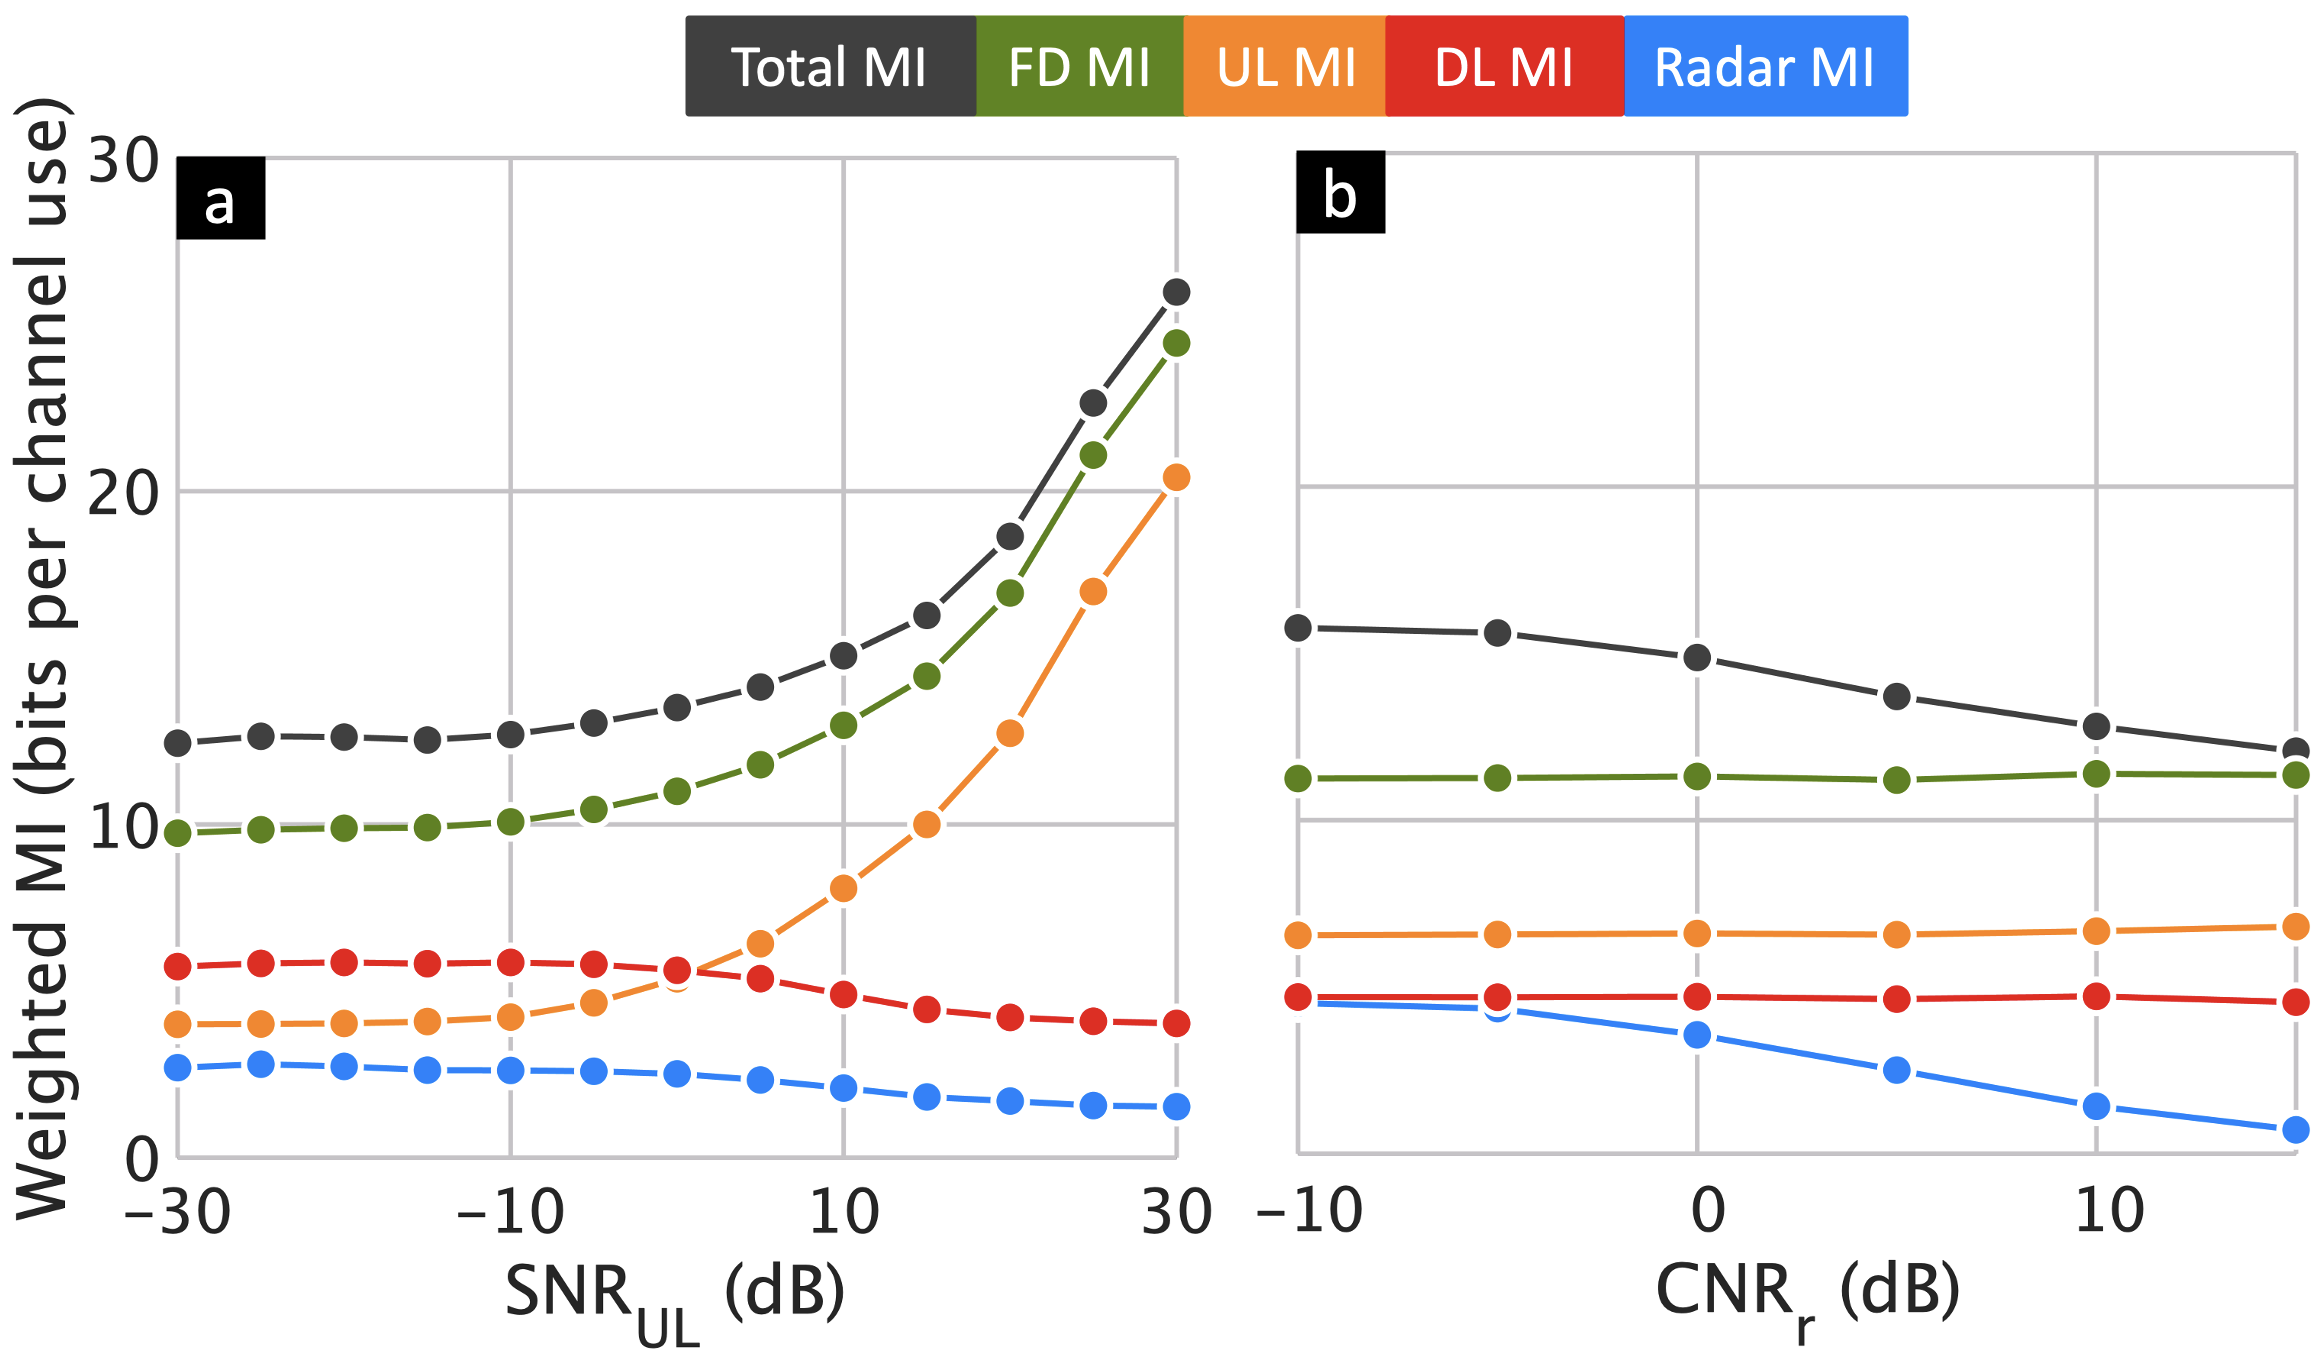
\includegraphics[width=0.9\columnwidth]{joint.png}
\caption{Joint radar and communications interference analysis. (a) System performance vs UL SNRs (b) System performance vs CNR.}
\label{fig:joint}
\vspace{-1em}
\end{figure}
\iffalse
%-------------------------------------------------------------
\begin{figure}[t]
\centering
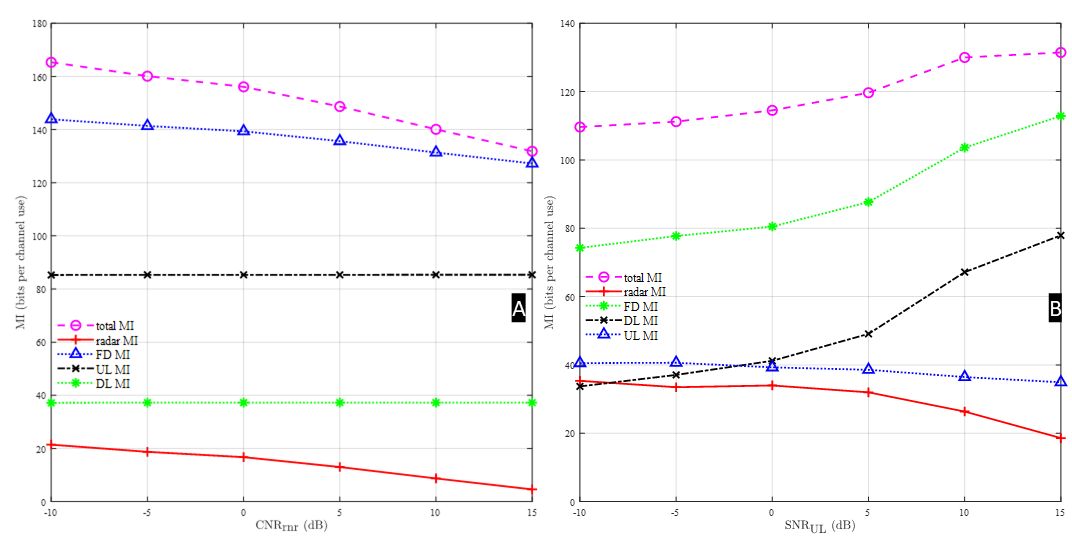
\includegraphics[width=1\columnwidth]{radar_figures_cnr.png}
%\vspace{-14pt}
\caption{$\paren{\textrm{a}}$ MI achieved by Algorithm $\ref{Alternating_sum}$ versus different $\mathrm{CNRs}$   $\paren{\textrm{b}}$ MI achieved by Algorithm $\ref{Alternating_sum}$ versus various UL $\mathrm{SNR}$ }
\label{fig:cnr}
\vspace{-1em}
\end{figure}
%-------------------------------------------------------------
\fi
We now explore the mutual impact of the statistical MIMO radar and FD MU-MIMO communications on each other. \figurename{\;\ref{fig:fd_vs_hd}} provides a comparison of the CWSMs achieved by the FD MU-MIMO as well as HD MU-MIMO communications systems while coexisting with the statistical MIMO radar. We also included the cooperation and noncooperation scenarios for the FD MU-MIMO and DL MU-MIMO communications. To make the simulation more practical, we assume that of the radar-enabled interference channel gains, namely $\eta^2_{\mathrm{r},j}$ and $\eta^2_{\mathrm{rB}}$ are fractions of the radar-target channel gains $\eta^2_{m\rr,n\rr}$. As a result, the severity of the radar-enabled interference with the communications systems are also related to the radar-target channel gains. Specifically, we set $\mathrm{SNR}_{\textrm{r}}=0.8\mathrm{SNR}_{\textrm{rB}}$ and $\mathrm{SNR}_{\textrm{r}}=0.6\mathrm{SNR}_{\textrm{rd}}$. We observe that when the radar power is dominating the co-existing system, the significance of the radar-DL cooperation is less apparent. In \figurename{\;\ref{fig:joint}}, we study how the co-existing system performance evolves with different UL SNR and CNR values.  %Like the assumption we made with \figurename{\;\ref{fig:fd_vs_hd}}, 
For this example, we assume that $\mathrm{SNR}_{\textrm{ur}}=0.7\mathrm{SNR}_{\textrm{u}}$ and  $\mathrm{SNR}_{\textrm{ud}}=0.8\mathrm{SNR}_{\textrm{u}}$ for \figurename{\;$\paren{\mathrm{\ref{fig:joint}}}$}a  and $\mathrm{SNR}_{\textrm{rB}}=0.5\mathrm{CNR}_{\textrm{r}}$ and $\mathrm{SNR}_{\textrm{rd}}=0.5\mathrm{CNR}_{\textrm{r}}$ for \figurename{\;$\paren{\mathrm{\ref{fig:joint}}}$}b.  \figurename{\;$\paren{\mathrm{\ref{fig:joint}}}$}a shows that the DL and radar weighted MIs declines by approximately $30\%$ and $45\%$, respectively, while the UL-DL and UL-radar interfering signal powers are $10^6$ times stronger, which demonstrates that the designed precoders and radar codes can sustain the DL and radar performances despite a high UL transmission power. Meanwhile, we can see the clutter is more impactful to the MIMO radar than the FD communications UEs from \figurename{\;$\paren{\mathrm{\ref{fig:joint}}}$}b, which is because the proposed method mitigates the power projected to the interfering channels $\mathbf{H}_{\textrm{rB}}$ and $\mathbf{H}_{\textrm{r,}j}$ from $\braces{\mathbf{a}\bracket{k}}$.
% $\eta_{\mathrm{u},i}$ and $\eta_{\mathrm{d},i}$ are fractions of $\eta^2_{i,n\rr}$ and $\eta_{m\rr,\B}$ and $\eta_{m\rr,j}$ are fractions of $\sigma^2_{\textrm{c},n\rr}$. 
\vspace{-1em}
%\section{Conclusion}
\section{Summary}
\label{sec:conclusion}
We presented a spectral co-design model consisting of a joint statistical MIMO radar and a FD-MU MIMO communications system and sequentially design the MIMO radar waveform code matrix, communications precoders as well as the linear receive filters for both radar and communications Rxs based on a BCU framework. The underlying novelty of the framework is that we exploit the relationship between the weighted sum-rate and the WMMSE so that the precoders and the sub-optimal radar codes can be found in closed-form expressions and we feed the obtained sub-optimal radar codes to a structured tight frame design method to find the optimal radar codes also satisfying the PAR constraints.  We then provide numerical examples to showcase that the statistical MIMO radar and FD MU-MIMO communications system can co-exist while maintaining their respective performances. We first demonstrate that the rapid convergence of Algorithm \ref{Alternating_sum} with an appropriate initialization. It is next shown that the radar codes produced by the proposed scheme boosts the probability of detection significantly compared to some conventional radar codes. The cooperation between the radar and DL signals is proved to be beneficial for the radar system. It is also illustrated that DL and radar performances are resilient to some considerable UL interference as well as the DL and UL rates remain stable as the CNR ascends given that the proposed precoders and radar codes are applied. Having shown our theoretical and numerical results, we conclude that our algorithm is a superior approach to achieve the spectral co-design for the co-existence of a statistical MIMO radar and a FD MU-MIMO communications system. For the future work, we would address the impact of the CSI errors on both the MIMO radar and FD MU-MIMO communications and develop a robust version of the proposed framework.
%such that the MIMO radar and the FD MU-MIMO communication system can operate simultaneously on the same spectrum while maintaining their respective performances.
	%  if have a single appendix:
	%\appendix[Proof of the Zonklar Equations]
	% or
	%\appendix  % for no appendix heading
	% do not use \section anymore after \appendix, only \section*
	% is possibly needed
	% use appendices with more than one appendix
	% then use \section to start each appendix
	% you must declare a \section before using any
	% \subsection or using \label (\appendices by itself
	% starts a section numbered zero.)
	%
	
\vspace{-1em}	
\appendices
\section{Taylor series approximation of the achievable rate}
\label{sec: appA}
One can express the first order approximation of a real-valued function with complex-valued matrix arguments $f\paren{\mathbf{X},\mathbf{X}^\ast}: \mathbb{C}^{\mathit{N}\times \mathrm{Q}}\times\mathbb{C}^{\mathit{N}\times \mathrm{Q}}\rightarrow\mathbb{R}$ with the Taylor series expansion at the point $\mathbf{X}_{\mathrm{0}}$ as \cite{hjorungnes2011complex} \par\noindent\small
\begin{flalign}
\label{eq: Taylor}
f\paren{\mathbf{X},\mathbf{X}^\ast} &= f\paren{\mathbf{X}_{\mathrm{0}},\mathbf{X}^\ast_{\mathrm{0}}}+\vect^\top\paren{\frac{\partial }{\partial \mathbf{X}_{\mathrm{0}}}f\paren{\mathbf{X}_{\mathrm{0}},\mathbf{X}^\ast_{\mathrm{0}}}}\vect\paren{\mathbf{X}-\mathbf{X}_{\mathrm{0}}}\nonumber\\
&+\vect^\top\paren{\frac{\partial }{\partial \mathbf{X}^\ast_{\mathrm{0}}}f\paren{\mathbf{X}_{\mathrm{0}},\mathbf{X}^\ast_{\mathrm{0}}}}\vect\paren{\mathbf{X}^\ast-\mathbf{X}^\ast_{\mathrm{0}}}.
\end{flalign}\normalsize
With $\paren{\ref{eq: Taylor}}$, one can show the first-order Taylor series of $\mathit{R}^\textrm{u}_{i}\bracket{k}$ evaluated at the initial approximation of $\PiB$, i.e., $\widetilde{\mathbf{P}}_{\textrm{u},i}\bracket{k}$, as \par\noindent\small
\begin{IEEEeqnarray}{rCl}
&&\mathit{R}^\textrm{u}_{q}\bracket{k}\paren{\PiB}\approx \mathit{R}^\textrm{u}_{q}\bracket{k}\paren{\widetilde{\mathbf{P}}_{\textrm{u},i}\bracket{k}}+\nonumber\\
&&\vect\braces{\frac{\partial \paren{\mathit{R}^\textrm{u}_{q}\bracket{k}\paren{\widetilde{\mathbf{P}}^\ast_{\textrm{u},i}\bracket{k}}}}{\partial \widetilde{\mathbf{P}}_{\textrm{u},i}\bracket{k}}}^\top\vect\braces{\PiB-\widetilde{\mathbf{P}}_{\textrm{u},i}\bracket{k}}+\nonumber\\
&&\vect\braces{\frac{\partial \paren{\mathit{R}^\textrm{u}_{q}\bracket{k}\paren{\widetilde{\mathbf{P}}_{\textrm{u},i}\bracket{k}}}}{\partial \widetilde{\mathbf{P}}^\ast_{\textrm{u},i}\bracket{k}}}^\top \vect\braces{\mathbf{P}^\ast_{\textrm{u},i}\bracket{k}-\widetilde{\mathbf{P}}^\ast_{\textrm{u},i}\bracket{k}}.
\end{IEEEeqnarray}\normalsize
where $\widetilde{\mathbf{P}}_{\textrm{u},i}\bracket{k}$ is regarded as the estimated value of $\PiB$ of the previous iteration for our proposed sequential algorithm.
Likewise, we can find the linear approximations of $\mathit{R}^\textrm{u}_{q}\bracket{k}\paren{\PBj}$, $\mathit{R}^\textrm{u}_{q}\bracket{k}\paren{\mathbf{a}\bracket{k}}$, $\mathit{R}^\textrm{d}_{g}\bracket{k}\paren{\PiB}$, $\mathit{R}^\textrm{d}_{g}\bracket{k}\paren{\PBj}$, and $\mathit{R}^\textrm{d}_{g}\bracket{k}\paren{\mathbf{a}\bracket{k}}$.
The derivatives of $f$ w.r.t. $\mathbf{X}^\ast$ can be thus approximated as \par\noindent\small
\begin{equation}
\label{eq: approxder}
\frac{\partial f}{\partial \mathbf{X}^\ast}=\frac{\partial }{\partial \mathbf{X}^\ast_{\mathrm{0}}}f\paren{\mathbf{X}_{\mathrm{0}},\mathbf{X}^\ast_{\mathrm{0}}}.
\end{equation}\normalsize
The chain rule for a scalar function $g\paren{\mathbf{U\paren{\mathbf{X},\mathbf{X}^\ast}},\mathbf{U}^\ast\paren{\mathbf{X},\mathbf{X}^\ast}}$ where $g$ is dependent on $\mathbf{X}^\ast$ through the matrix $\mathbf{U}$ can be written as \cite{IMM2012-03274}\par\noindent\small
\begin{flalign}
\label{eq: chainrule}
\frac{\partial g}{\partial \mathbf{X}^\ast}=\frac{\trace\braces{\paren{\frac{\partial g }{\partial \mathbf{U}}}^\top\partial \mathbf{U}}}{\partial \mathbf{X}^\ast} + \frac{\trace\braces{\paren{\frac{\partial g }{\partial \mathbf{U}^\ast}}^\top\partial \mathbf{U}^\ast}}{\partial \mathbf{X}^\ast}.
\end{flalign}\par\noindent\small
Utilizing $\paren{\ref{eq: approxder}}$, $\paren{\ref{eq: chainrule}}$, the derivative of the logarithm of determinant formula $\partial\log\left|\mathbf{X}\right|=\trace\braces{\mathbf{X}^{-1}\partial\mathbf{X}}$ \cite{hjorungnes2011complex,IMM2012-03274}, as well as  one can obtain the derivatives of $\mathit{R}^\textrm{u}_{q}\bracket{k}$ and $\mathit{R}^\textrm{d}_{g}\bracket{k}$ w.r.t. $\PiB$, $\PBj$, and $\mathbf{a}\bracket{k}$ based on their Taylor series expansions in the initial approximations of $\PiB$, $\PBj$, and $\mathbf{a}\bracket{k}$, denoted by $\widetilde{\mathbf{P}}_{\textrm{u},i}\bracket{k}$, $\widetilde{\mathbf{P}}_{\textrm{d},j}\bracket{k}$, and $\widetilde{\mathbf{a}}\bracket{k}$, respectively, as\par\noindent\small
\begin{flalign}
\nabla_{\PiB}\mathit{R}^\textrm{u}_{q}\bracket{k}=&\HiBH\boldsymbol{\Psi}_{\textrm{u},i}\widetilde{\mathbf{P}}_{\textrm{u},i}\bracket{k}\boldsymbol{\Upsilon}^{-1}_{\textrm{u},i}, ~q=i,\nonumber\\
\nabla_{\mathbf{P}_{\textrm{u},i}\bracket{k}}\mathit{R}^\textrm{u}_{q}\bracket{k}=&-\HiBH\boldsymbol{\Psi}_{\textrm{u},q}\PqB\boldsymbol{\Upsilon}^{-1}_{\textrm{u},q}\nonumber\\
&\PqBH\boldsymbol{\Psi}^\dagger_{\textrm{u},q}\HiB\widetilde{\mathbf{P}}_{\textrm{u},i}\bracket{k},~q\neq i,\nonumber\\
\nabla_{\PBj}\mathit{R}^\textrm{u}_{q}\bracket{k}=&-\HBBH\boldsymbol{\Psi}_{\textrm{u},q}\PqB\boldsymbol{\Upsilon}^{-1}_{\textrm{u},q}\PqBH\boldsymbol{\Psi}^\dagger_{\textrm{u},q}\HBB{\mathbf{P}}_{\textrm{d},j}\bracket{k},\nonumber\\
\nabla_{\mathbf{a}\bracket{k}}\mathit{R}^\textrm{u}_{q}\bracket{k}=&-\HrBH\boldsymbol{\Psi}_{\textrm{u},q}\PqB\boldsymbol{\Upsilon}^{-1}_{\textrm{u},q}\PqBH\boldsymbol{\Psi}^\dagger_{\textrm{u},q}\HrB\mathbf{a}\bracket{k}, \nonumber\\
\nabla_{\PiB}\mathit{R}^\textrm{d}_{g}\bracket{k}=&-\mathbf{H}^\dagger_{i,g}\boldsymbol{\Psi}_{\textrm{d},g}\PBg\boldsymbol{\Upsilon}^{-1}_{\textrm{d},g}\PBgH\boldsymbol{\Psi}^\dagger_{\textrm{d},g}\mathbf{H}_{i,g}\widetilde{\mathbf{P}}_{\textrm{u},i}\bracket{k},\nonumber\\
\nabla_{\PBj}\mathit{R}^\textrm{d}_{g}\bracket{k}=&\mathbf{H}^\dagger_{\B,j}\boldsymbol{\Psi}_{\textrm{d},j}\widetilde{\mathbf{P}}_{\textrm{d},j}\bracket{k}\boldsymbol{\Upsilon}^{-1}_{\textrm{d},j}, g=j,\nonumber\\
\nabla_{\PBj}\mathit{R}^\textrm{d}_{g}\bracket{k}=&-\HBjH\boldsymbol{\Psi}_{\textrm{d},g}\PBg\boldsymbol{\Upsilon}^{-1}_{\textrm{d},g},\nonumber\\
&\PBgH\boldsymbol{\Psi}^\dagger_{\textrm{d},g}\HBj\widetilde{\mathbf{P}}_{\textrm{d},j}\bracket{k}, ~g\neq j,\nonumber\\
\nabla_{\mathbf{a}\bracket{k}}\mathit{R}^\textrm{d}_{g}\bracket{k}=&-\mathbf{H}^\dagger_{\textrm{r},g}\boldsymbol{\Psi}_{\textrm{d},g}\PBg\boldsymbol{\Upsilon}^{-1}_{\textrm{d},j}\PBgH\boldsymbol{\Psi}^\dagger_{\textrm{d},g}\mathbf{H}_{\textrm{r},g}\mathbf{a}\bracket{k}, 
\end{flalign}
\begin{align}
\textrm{where }\boldsymbol{\Upsilon}_{\textrm{u},i}\bracket{k}&=\mathbf{I}+\widetilde{\mathbf{P}}^\dagger_{\textrm{u},i}\bracket{k}\mathbf{H}^\dagger_{i,\textrm{B}}\Riniin\mathbf{H}_{i,\textrm{B}}\widetilde{\mathbf{P}}_{\textrm{u},i}\bracket{k}\nonumber\\
\boldsymbol{\Upsilon}_{\textrm{u},q}&=\mathbf{I}+\PqBH\HqBH\Rinqin \HqB\PqB,q\neq i\nonumber\\
\boldsymbol{\Upsilon}_{\textrm{d},g}&=\mathbf{I}+ \widetilde{\mathbf{P}}^\dagger_{\textrm{d},j}\bracket{k}\HBjH \Rinjin\HBj\widetilde{\mathbf{P}}_{\textrm{d},j}\bracket{k},\nonumber\\
\boldsymbol{\Upsilon}_{\textrm{d},g}&= \mathbf{I}+\PBgH\HBgH\Ringin\HBg\PBg, g\neq j,\nonumber\\
\boldsymbol{\Psi}_{\textrm{u},q}&=\Rinqin\textrm{ and }\boldsymbol{\Psi}_{\textrm{d},g}=\Ringin\HBg.\nonumber
\end{align}\normalsize
\iffalse
$\boldsymbol{\Upsilon}_{\textrm{u},i}\bracket{k}=\mathbf{I}+\widetilde{\mathbf{P}}^\dagger_{\textrm{u},i}\bracket{k}\mathbf{H}^\dagger_{i,\textrm{B}}\Riniin\mathbf{H}_{i,\textrm{B}}\widetilde{\mathbf{P}}_{\textrm{u},i}\bracket{k}$, $\boldsymbol{\Upsilon}_{\textrm{u},q}=$ $\mathbf{I}+$ $\PqBH\HqBH\Rinqin$ $\HqB\PqB,$ $q\neq i$, $\boldsymbol{\Upsilon}_{\textrm{d},g}=$ $\mathbf{I}+$ $\widetilde{\mathbf{P}}^\dagger_{\textrm{d},j}\bracket{k}\HBjH$ $\Rinjin\HBj\widetilde{\mathbf{P}}_{\textrm{d},j}\bracket{k}$, $\boldsymbol{\Upsilon}_{\textrm{d},g}=$ $\mathbf{I}+\PBgH\HBgH\Ringin\HBg\PBg$, $g\neq j$,\fi %$\boldsymbol{\Psi}_{\textrm{u},q}=\Rinqin\HqB$, and $\boldsymbol{\Psi}_{\textrm{d},g}=\Ringin\HBg$.
\iffalse
	\begin{figure*}[t]
		\par\noindent\small
		\begin{flalign}
		&\nabla_{\PiB}\mathit{R}^\textrm{u}_{q}\bracket{k}=\HiBH\Riniin\HiB\widetilde{\mathbf{P}}_{\textrm{u},i}\bracket{k}\paren{\mathbf{I}+\widetilde{\mathbf{P}}^\dagger_{\textrm{u},i}\bracket{k}\mathbf{H}^\dagger_{i,\textrm{B}}\Riniin\mathbf{H}_{i,\textrm{B}}\widetilde{\mathbf{P}}_{\textrm{u},i}\bracket{k}}^{-1} ~q=i,
		\end{flalign}
		\begin{flalign}
		&\nabla_{\mathbf{P}_{\textrm{u},i}\bracket{k}}\mathit{R}^\textrm{u}_{q}\bracket{k}=-\HiBH\Rinqin\HqB\PqB\paren{\mathbf{I}+\mathbf{P}^\dagger_{q,\textrm{B}}\bracket{k}\mathbf{H}^\dagger_{q,\textrm{B}}\Rinqin\mathbf{H}_{q,\textrm{B}}\mathbf{P}_{q,\textrm{B}}\bracket{k}}^{-1}\nonumber\\
		&\;\;\qquad\qquad\qquad\qquad\PqBH\HqBH\Rinqin\HiB\widetilde{\mathbf{P}}_{\textrm{u},i}\bracket{k},~q\neq i\nonumber
		\end{flalign}
		\begin{flalign}
		&\nabla_{\PiB}\mathit{R}^\textrm{d}_{g}\bracket{k}=-\mathbf{H}^\dagger_{i,g}\Ringin\HBg\PBg\paren{\mathbf{I}+\PBjH\bracket{k}\mathbf{H}^\dagger_{\textrm{B},g}\Ringin\mathbf{H}_{\textrm{B},g}\PBg}^{-1}\PBgH\HBgH\Ringin\mathbf{H}_{i,g}\widetilde{\mathbf{P}}_{\textrm{u},i}\bracket{k},\nonumber\\
		&\nabla_{\PBj}\mathit{R}^\textrm{d}_{g}\bracket{k}=\mathbf{H}^\dagger_{\B,j}\paren{\Rinj}^{-1}\HBj\PBj\paren{\mathbf{I}+\PBjH\bracket{k}\mathbf{H}^\dagger_{\textrm{B},j}\Rinjin\mathbf{H}_{\textrm{B},j}\PBj}^{-1}, g=j,\\
		&\nabla_{\PBj}\mathit{R}^\textrm{d}_{g}\bracket{k}=-\HBjH\Ringin\HBg\PBg\paren{\mathbf{I}+\mathbf{P}^\dagger_{\textrm{B},g}\bracket{k}\mathbf{H}^\dagger_{\textrm{B},g}\Ringin\mathbf{H}_{\textrm{B},g}\mathbf{P}_{\textrm{B},g}\bracket{k}}^{-1}\PBgH\HBgH\Ringin\HBj\widetilde{\mathbf{P}}_{\textrm{d},j}\bracket{k} ~g\neq j\nonumber\\
		&\nabla_{\PBj}\mathit{R}^\textrm{u}_{q}\bracket{k}=-\HBBH\Rinqin\HqB\PqB\paren{\mathbf{I}+\PqBH\mathbf{H}^\dagger_{i,\textrm{B}}\Rinqin\HqB\PqB}^{-1}\nonumber\\
		&\PqBH\HqBH\Rinqin\HBB{\mathbf{P}}_{\textrm{d},j}\bracket{k},\\
		&\nabla_{\mathbf{a}\bracket{k}}\mathit{R}^\textrm{u}_{q}\bracket{k}=-\HrBH\Rinqin\HqB\PqB\paren{\mathbf{I}+\PqBH\mathbf{H}^\dagger_{i,\textrm{B}}\Rinqin\HqB\PqBH}^{-1}\PqBH\HqBH\Rinqin\HrB\mathbf{a}\bracket{k},\\
		&\nabla_{\mathbf{a}\bracket{k}}\mathit{R}^\textrm{d}_{g}\bracket{k}=-\mathbf{H}^\dagger_{\textrm{r},g}\Ringin\HBg\PBg\paren{\mathbf{I}+\PBgH\HBgH\Ringin\HBg\PBg}^{-1}\PBgH\HBgH\Ringin\mathbf{H}_{\textrm{r},g}\mathbf{a}\bracket{k}.
		\end{flalign}\normalsize
	\end{figure*}
\fi
	\iffalse 
	\begin{figure*}[b!]
		\par\noindent\small
		\begin{flalign}
		\IEEEyesnumber\IEEEyessubnumber*
		\mathit{R}^\textrm{u}_{q}\bracket{k}\paren{\PiB}&\approx \mathit{R}^\textrm{u}_{q}\bracket{k}\paren{\widetilde{\mathbf{P}}_{\textrm{u},i}\bracket{k}}+ \trace\braces{\paren{\nabla_{\widetilde{\mathbf{P}}_{\textrm{u},i}\bracket{k}}\mathit{R}^\textrm{u}_{q}\bracket{k}}^\dagger\PiB}  -\trace\braces{\paren{\nabla_{\widetilde{\mathbf{P}}_{\textrm{u},i}\bracket{k}}\mathit{R}^\textrm{u}_{q}\bracket{k}}^\dagger\widetilde{\mathbf{P}}_{\textrm{u},i}\bracket{k}}\\
		\mathit{R}^\textrm{u}_{q}\bracket{k}\paren{\PBj}&\approx \trace\braces{\paren{\nabla_{\widetilde{\mathbf{P}}_{\B,j}\bracket{k}}\mathit{R}^\textrm{u}_{q}\bracket{k}}^\dagger\PBj}+\mathit{R}^\textrm{u}_{q}\bracket{k}\paren{\widetilde{\mathbf{P}}_{\B,j}\bracket{k}}-\trace\braces{\paren{\nabla_{\widetilde{\mathbf{P}}_{\B,j}\bracket{k}}\mathit{R}^\textrm{u}_{q}\bracket{k}}^\dagger\widetilde{\mathbf{P}}_{\B,j}\bracket{k}}\\
		\mathit{R}^\textrm{u}_{q}\bracket{k}\paren{\mathbf{a}\bracket{k}}&\approx\trace\braces{\paren{\nabla_{\widetilde{\mathbf{a}}\bracket{k}}\mathit{R}^\textrm{u}_{q}\bracket{k}}^\dagger\mathbf{a}\bracket{k}}+\mathit{R}^\textrm{u}_{q}\bracket{k}\paren{\widetilde{\mathbf{a}}\bracket{k}}-\trace\braces{\paren{\nabla_{\widetilde{\mathbf{a}}\bracket{k}}\mathit{R}^\textrm{u}_{q}\bracket{k}}^\dagger\widetilde{\mathbf{a}}\bracket{k}}\\
		\mathit{R}^\textrm{d}_{g}\bracket{k}\paren{\PiB}&\approx \trace\braces{\paren{\nabla_{\widetilde{\mathbf{P}}_{\textrm{u},i}\bracket{k}}\mathit{R}^\textrm{d}_{g}\bracket{k}}^\dagger\PiB}+\mathit{R}^\textrm{d}_{g}\bracket{k}\paren{\widetilde{\mathbf{P}}_{\textrm{u},i}\bracket{k}}-\trace\braces{\paren{\nabla_{\widetilde{\mathbf{P}}_{\textrm{u},i}\bracket{k}}\mathit{R}^\textrm{d}_{g}\bracket{k}}^\dagger\widetilde{\mathbf{P}}_{\textrm{u},i}\bracket{k}}\\
		\mathit{R}^\textrm{d}_{g}\bracket{k}\paren{\PBj}&\approx \trace\braces{\paren{\nabla_{\widetilde{\mathbf{P}}_{\B,j}\bracket{k}}\mathit{R}^\textrm{d}_{g}\bracket{k}}^\dagger\PBj}+\mathit{R}^\textrm{d}_{g}\bracket{k}\paren{\widetilde{\mathbf{P}}_{\B,j}\bracket{k}}-\trace\braces{\paren{\nabla_{\widetilde{\mathbf{P}}_{\B,j}\bracket{k}}\mathit{R}^\textrm{d}_{g}\bracket{k}}^\dagger\widetilde{\mathbf{P}}_{\B,j}\bracket{k}}\\
		\mathit{R}^\textrm{d}_{g}\bracket{k}\paren{\mathbf{a}\bracket{k}}&\approx\trace\braces{\paren{\nabla_{\widetilde{\mathbf{a}}\bracket{k}}\mathit{R}^\textrm{d}_{g}\bracket{k}}^\dagger\mathbf{a}\bracket{k}}+\mathit{R}^\textrm{d}_{g}\bracket{k}\paren{\widetilde{\mathbf{a}}\bracket{k}}-\trace\braces{\paren{\nabla_{\widetilde{\mathbf{a}}\bracket{k}}\mathit{R}^\textrm{d}_{g}\bracket{k}}^\dagger\widetilde{\mathbf{a}}\bracket{k}}.
		\end{flalign}\normalsize
		%	\end{widetext}
	\end{figure*}
	\fi
	%as well as the identities $\trace\braces{\mathbf{AJ}^{ij}\mathbf{B}}=\paren{\mathbf{A}^\dagger\mathbf{B}^\dagger}\paren{i,j}$ and $\trace\braces{\mathbf{AJ}^{ji}\mathbf{B}}=\paren{\mathbf{B}\mathbf{A}}\paren{i,j}$, where $\mathbf{J}^{ij}$ denotes a single entry matrix with the $\ith{\paren{i,j}}$ element to be $1$ and zero elsewhere\cite{IMM2012-03274}, i.e., Retaining only the linear terms of the expansions,
	%	\begin{widetext}
	%\begin{figure*}[b]
	%		\par\noindent\small
	%\begin{flalign}
	%&\nabla_{\PiB}\mathit{R}^\textrm{u}_{q}\bracket{k}=-2\HqBH\Rinqin\HqB\PqB\paren{\mathbf{I}+\mathbf{P}^\dagger_{q,\textrm{B}}\bracket{k}\mathbf{H}^\dagger_{q,\textrm{B}}\Rinqin\mathbf{H}_{q,\textrm{B}}\mathbf{P}_{q,\textrm{B}}\bracket{k}}^{-1}\PqBH\HqBH\Rinqin\HiB\PiB,\\
	%&\nabla_{\PBj}\mathit{R}^\textrm{d}_{g}\bracket{k}=-2\HBgH\Ringin\HBg\PBg\paren{\mathbf{I}+\mathbf{P}^\dagger_{\textrm{B},g}\bracket{k}\mathbf{H}^\dagger_{\textrm{B},g}\Ringin\mathbf{H}_{\textrm{B},g}\mathbf{P}_{\textrm{B},g}\bracket{k}}^{-1}\PBgH\HBgH\Ringin\HBg\PBj.
	%\end{flalign}\normalsize
	%\end{figure*}
	
	%	\end{widetext}
	%-------------------------------------------------------------
	%\begin{algorithm}[t]
	%	\caption{Target Recovery via TenDSuR OMP}
	%	\label{Alg:OMP}
	%	\begin{algorithmic}[1]
	%		\Statex \textbf{Input:}
	%		$\mathrm{\iota+1}$,  $\bar{\mathcal{Z}}$, $L$
	%		\Statex \textbf{Output:}
	%		Estimated support $\hat{\Phi}$ of $\mathcal{X}$, sparse estimate $\hat{\mathcal{X}}$
	%		\State (\textit{Initialization}): $\mathcal{R}=\bar{\mathcal{Z}}$, $\Phi_0={\emptyset}$, $i=1$;
	%		\State (\textit{Projection}): $\mathcal{Y} = [\![\mathcal{R}; \mathbf{A}^H, \mathbf{B}^H, \mathbf{F}^H]\!]$;
	%		\State (\textit{Support set augmentation}): $\Phi_i=\Phi_{i-1}\cup \{\phi_i\}$, where
	%		\par\noindent \small\begin{equation}
	%		\phi_i=\big\{\phi_{i}(1),\phi_{i}(2),\phi_{i}(3)\big\} =\arg\max_{\{s_1,s_2,s_3\}}\big|[\mathcal{Y}]_{s_1,s_2,s_3}\big|;\nonumber
	%		\end{equation}\normalsize
	%		\State (\textit{Residual}):
	%		\small
	%		$
	%		\mathcal{R} = \bar{\mathcal{Z}}-\mathcal{P}_{\mathrm{\iota+1}}\left\{\sum_{l=1}^{i}[{\alpha}_i]_l \cdot \left([\mathbf{A}]_{\phi_{l}(1)}\circ[\mathbf{B}]_{\phi_{l}(2)}\circ[\mathbf{F}]_{\phi_{l}(3)}\right)\right\}$;\normalsize
	%		\State (\textit{Iteration}): if $i < L$, $i=i+1$ and go to Step 2, else stop;
	%		\State (\textit{Output}): $\hat{\Phi} = \Phi_L$; $\hat{\mathcal{X}}\in \mathbb{C}^{TN\times TR\times P}$, where
	%		\par\noindent \small\begin{equation}
	%		[\hat{\mathcal{X}}]_{\phi_{l}(1),\phi_{l}(2),\phi_{l}(3)} =\left\{\begin{array}{cc}
	%		[{\alpha}]_l, &l=1,2,\dots, L,\nonumber\\
	%		0, &\mbox{otherwise.}
	%		\end{array}   \right.
	%		\end{equation}\normalsize
	%	\end{algorithmic}
	%\end{algorithm}
	%-------------------------------------------------------------
	%	\begin{IEEEeqnarray}{rCl}\label{diagonal MMSE radar }
	%	\mathbf{E}\rnr\bracket{k}&=&\mathbb{E}\braces{\paren{\mathbf{h}_{\mathrm{t},n\rr}-\mathbf{u}\rnr\bracket{k}\mathbf{y}\rnr\bracket{k}}\paren{\mathbf{h}_{\mathrm{t},n\rr}-\mathbf{u}\rnr\bracket{k}\mathbf{y}\rnr\bracket{k}}^\dagger}\nonumber\\
	%	&=&\eta^2_\target\mathbf{I}-2\eta^2_\target\mathbf{s}_{\mathrm{t},n\rr}\bracket{k}\mathbf{u}^\dagger\rnr\bracket{k}+\mathbf{u}\rnr\bracket{k}\mathit{R}_{\target,n\rr}\bracket{k}\mathbf{u}^\dagger\rnr\bracket{k}+\mathbf{u}\rnr\bracket{k}\mathit{R}_{\mathrm{in},n\rr}\bracket{k}\mathbf{u}^\dagger\rnr\bracket{k}\nonumber\\
	%	&=&\eta^2_\target\mathbf{I}-2\eta^2_\target\paren{\mathbf{Q}\rnr\bracket{k}\mathbf{a}\bracket{k}+\mathbf{q}_{\mathrm{Bt},n\rr}\bracket{k}\sum_{j=1}^{\mathit{J}}\PBj\mathbf{d}_{\B,j}\bracket{k}}\mathbf{u}^\dagger\rnr\bracket{k}+\eta^2_\target\mathbf{u}\rnr\bracket{k}\nonumber\\
	%	&&\paren{\mathbf{a}^\dagger\bracket{k}\mathbf{Q}^\dagger\rnr\bracket{k}+\mathbf{q}^\ast_{\mathrm{Bt},n\rr}\bracket{k}\sum_{j=1}^J\mathbf{d}^\dagger_{\B,j}\bracket{k}\PBjH}\paren{\mathbf{Q}\rnr\bracket{k}\mathbf{a}\bracket{k}+\mathbf{q}_{\mathrm{Bt},n\rr}\bracket{k}\sum_{j=1}^J\PBj\mathbf{d}_{\B,j}\bracket{k}}\mathbf{u}^\dagger\rnr\bracket{k}\nonumber\\
	%	&&\mathbf{u}\rnr\bracket{k}\left( 
	%	\sizecorr{+\sum_{i=1}^{\mathit{I}}\eta^2_i\mathbf{d}^\dagger_{i,\B}\bracket{k}\PiBH\PiB\mathbf{d}_{i,\B}\bracket{k}}
	%	\mathbf{a}^\dagger\bracket{k}\mathbf{a}\bracket{k}\trace\braces{\mathbf{R}_{\mathrm{c},n\rr}}+\sigma^2\rnr\mathbf{u}^\dagger\rnr\bracket{k}+\eta^2_\B\paren{\sum_{j=1}^{\mathit{J}}\mathbf{d}^\dagger_{\B,j}\bracket{k}\PBjH}\paren{\sum_{j=1}^{\mathit{J}}\PBj\mathbf{d}_{\B,j}\bracket{k}}\right.\nonumber\\
	%	&&\left.+\sum_{i=1}^{\mathit{I}}\eta^2_i\mathbf{d}^\dagger_{i,\B}\bracket{k}\PiBH\PiB\mathbf{d}_{i,\B}\bracket{k}\right)\mathbf{u}^\dagger\rnr\bracket{k}
	%\end{IEEEeqnarray}
	%\section{Proof of Theorem $\mathrm{\ref{MMSE_MItheorem}}$ }\label{theorem1proof}
	% you can choose not to have a title for an appendix
	% if you want by leaving the argument blank
	
	%\section{}
	%Appendix two text goes here.
	
	
	\clearpage
%	\textcolor{red}{Vijay: I will reduce the references to only one page so that we have more space for technical writing.}
	\bibliographystyle{IEEEtran}
	\bibliography{IEEEabrv,Codesign_MIMO_RadComm_bibfile}
	
\end{document}


